

%==============================================================================
% TEMPLATE FOR THESIS WAGENINGEN UNIVERSITY
% CREATED BY AREND LIGTENBERG JUNE 2006;
% EDITED BY KIM CALDERS 2014;
% EDITED BY BEN DEVRIES 2015;
% EDITED BY LOIC DUTRIEUX 2016
% EDITED BY SIMON FRAVAL 2018
%==============================================================================

\documentclass [a4paper,11pt,twoside]{book} %convert to booklet size through shell script
%Text spans 14.3cm across

%%%Additional packages by Simon
%\usepackage{longtable} %split tables over multiple pages
\usepackage{booktabs} %included for lines at the top and bottom of tables
\usepackage{arydshln} %for dotted lines \hdashline
%\usepackage{wrapfig} %for wraping test around figures or tables
\usepackage{enumitem} %Used in chapter 2 for lists.
\usepackage{upgreek} %Used for greek letters in chaper 3
\usepackage[table]{xcolor} %for grey midrules. See here: https://tex.stackexchange.com/questions/317077/lighter-midrule %This needs to be above some other package below otherwise there is a clash. Probably with \usepackage{colour}

%\usepackage[hidelinks]{hyperref} %Make all references clickable, but without a red box around it.
%integrate this. See here: https://tex.stackexchange.com/questions/26529/how-can-i-generate-pdf-metadata-from-latex
\usepackage[hidelinks, pdftex,
            pdfauthor={Simon Fraval},
            pdftitle={Food security in rural sub-Saharan Africa: A household level assessment of crop-livestock systems},
            pdfsubject={Rural livelihoods},
            pdfkeywords={Food security, micronutrients, livelihoods},
            pdfproducer={Lualatex},
            pdfcreator={Lualatex}]{hyperref}

%%%%%%Original packages with notes from Simon
%\usepackage[utf8]{inputenc} %use this if special characters are in the reference list.
\usepackage[dutch,english]{babel}
\usepackage{graphicx}
\usepackage[authoryear]{natbib} %for reference management. Easy intext citation with \citealp, or \citet ect. %An alternative is to use biber: https://en.wikibooks.org/wiki/LaTeX/Bibliographies_with_biblatex_and_biber
%\usepackage{bibentry} % bibentry for inserting complete BibTeX entries inline, explanation: http://stefaanlippens.net/bibentry
%\nobibliography* % required by bibentry package;
%\usepackage{luabibentry}
%\setupbibentry{\jobname} %\jobname if named the same as main file %Enter chapter refs manually
\usepackage{amsmath}
\usepackage{fancyhdr}
\usepackage[small,bf]{caption}
%\captionsetup[table]{skip=10pt}
\captionsetup{labelsep=space} % Just have a space after caption number. No colon. Can use labelsep=period too. See https://tex.stackexchange.com/questions/29181/figure-and-table-numbers-in-caption-are-terminated-by-a-period-and-semicolon
\usepackage{multirow}
\usepackage{threeparttable} % Good for adding notes to table.
%\usepackage[body={6.0in, 8.2in},left=1.50in,right=1.50in]{geometry} %% very narrow
\usepackage[top=3.35cm, bottom=3.35cm, left=2.5cm, right=2.5cm]{geometry}
\usepackage[parfill]{parskip}
\usepackage{pdfpages}
\usepackage{color}
\usepackage{appendix}

% extra packages added by Ben
\usepackage[figuresright]{rotating} %!Put rotate all sideways tables in the same direction with the top to the left
\usepackage{changepage} % for indenting entire paragraphs
\usepackage{float} % help with table positioning
\floatstyle{plaintop} % caption on top
\restylefloat{table} % see above. Use: \begin{table}[H]
\usepackage{textcomp} % \textdegree
\usepackage{csquotes} % for block quotes, use {displayquote} environment
%\usepackage{todonotes}
\usepackage{soul}
\usepackage{fp}
\usepackage{tabularx}
\newcolumntype{Y}{>{\centering\arraybackslash}X} %centre columns in tabularx environment
\newcolumntype{L}[1]{>{\raggedright\arraybackslash}p{#1}} %left align fixed width column in tabular environment
\newcolumntype{C}[1]{>{\centering\arraybackslash}p{#1}} % center a fixed with column in tabular environment
\usepackage{subcaption}
\usepackage{pdflscape} %Use for sideways table with longtable
\usepackage{hvfloat} %For rotating tables with more control
\usepackage{gensymb}
\usepackage[version=4]{mhchem}
\usepackage{wrapfig}
\usepackage{makecell} %For controlling text in a table cell. See: https://tex.stackexchange.com/questions/2441/how-to-add-a-forced-line-break-inside-a-table-cell
\usepackage{lastpage} %To refer to the last page with automatic update
\usepackage{lipsum} %For adding dummy text to the ducument - for testing purposes
%\usepackage{pstricks} %For adding full page images between sections
\usepackage{graphicx} %Full page image

\providecommand\phantomsection{} %Hyperref to find the right page https://tex.stackexchange.com/questions/44088/when-do-i-need-to-invoke-phantomsection

\addto\captionsenglish{\renewcommand{\bibname}{References}}



\definecolor{Red}{rgb}{0.5,0,0}
\definecolor{Blue}{rgb}{0,0,0.5}

%%%%%%%%%%%%%%%%%%%%%%%%%%%%%%%%%%%%%%%%%%%%%%%%%%%%%%%%%%
%=======================================================================
% GENERAL SETTINGS
%=======================================================================

\setlength{\captionmargin}{5pt}


\linespread{1.15} %1 is single spacing, 1.3 is oneandhalf spacing

%% for internal use
\newcommand{\fixme}[1]{\emph{\marginpar{FIXME} (#1)}}
\newcommand{\readme}[1]{\emph{\marginpar{README} (#1)}}
\newcommand{\verifyme}[1]{\emph{\marginpar{VERIFYME} (#1)}}


%=======================================================================
% DEFINITION OF THE FANCY HEADERS %Revised S.F. 2018
%=======================================================================
\pagestyle{fancy}
\renewcommand{\chaptermark}[1]{\markboth{#1}{}}
\renewcommand{\sectionmark}[1]{\markright{\thesection\ #1}}
\fancyhf{}
\fancyhead[LE,RO]{\footnotesize\sffamily\thepage} %!\bfseries put before \thepage \rightmark \leftmark if you want a bold running head
\fancyhead[LO]{\footnotesize\sffamily\rightmark} %!My preference was for a smaller running head with the same font and the headings
\fancyhead[RE]{\footnotesize\sffamily\leftmark}
%\fancyfoot[LE,CE,RE]{\scriptsize{Draft: June 2006}}
%\fancyfoot[LO,CO,RO]{\scriptsize{Draft: June 2006}}
\headheight 15pt

\fancypagestyle{plain}{%
\fancyhead{} % get rid of headers
\renewcommand{\headrulewidth}{0pt} % and the line
}
\renewcommand{\headrulewidth}{0.4pt}
%\renewcommand{\footrulewidth}{0.4pt}

%!Does not work with LuaLATEX
%\pdfinfo{
 %  /Author (Simon Fraval)
   %/Title  (Food security in rural sub-Saharan Africa: A household level assessment of crop-livestock systems)
   %/CreationDate (D:Date)
%}

%=======================================================================
% NEW ENVIRONMENT FOR THE START OF CHAPTER (SMALL ABSTRACT)
%=======================================================================
\newenvironment{chapintro}
{
    \begin{center}
    \begin{minipage}[t]{0.9\textwidth}
    \hrule
    \medskip
    \small
}
{
    \medskip
    \hrule
    \end{minipage}
    \end{center}
    \bigskip
}


%=======================================================================
% Adjust TOC  %Revised. S.F. 2018
%=======================================================================

%TOC text wrapping: https://tex.stackexchange.com/questions/394227/memoir-toc-indent-the-second-line-by-numberspace-width-in-the-previous-line-or
%https://tex.stackexchange.com/questions/16032/how-do-i-indent-the-2nd-line-a-long-chapter-name-created-using-the-tocloft-packa
%Align wrapped text
%Add the word `Chapter' to the start
%Add dots

\usepackage{tocloft}

\renewcommand{\cftbeforechapskip}{\baselineskip}      % allow spacing after each chapter/section entry
\renewcommand{\contentsname}{Contents}
%\addto\captionsenglish{\def\contentsname{Contents}} %! Needed for babel? https://tex.stackexchange.com/questions/35903/formatting-the-title-of-the-toc
\renewcommand{\cfttoctitlefont}{\hfill\Large\bfseries\sffamily} %!some command to make the heading huge and bold
\renewcommand{\cftaftertoctitle}{\hfill}
\renewcommand{\cftbeforetoctitleskip}{-0.25in}        % Title is 1in from top
\renewcommand{\cftaftertoctitleskip}{2.0\baselineskip}% 1 double space after title
%\renewcommand{\cftaftertoctitle}{ \\[\baselineskip]\mbox{}\hfill{\normalfont Page}}
\renewcommand{\cftchapfont}{\sffamily}                         % Can make it bold faced here
\renewcommand{\cftchappagefont}{\sffamily}                         % Can make it bold faced here
\renewcommand{\cftchapleader}{\cftdotfill{\cftchapdotsep}}
\renewcommand{\cftchapdotsep}{\cftdotsep}             % Puts dots after chapter entries
\renewcommand{\cftchappresnum}{Chapter\ }             %
\renewcommand{\cftchapaftersnum}{}                    %
\renewcommand{\cftsecleader}{\cftdotfill{\cftsecdotsep}}%
\renewcommand{\cftchapnumwidth}{1in}


%=======================================================================
% A BIT MORE COMPACT ITEM LIST
%=======================================================================
\newenvironment{itemize*}%
  {\begin{itemize}%
    \setlength{\parskip}{0pt}%
    \setlength{\itemsep}{0pt}%
    \setlength{\parsep}{0pt}}%
  {\end{itemize}}


%=======================================================================
% A BIT MORE COMPACT DESCRIPTION LIST
%=======================================================================
\renewcommand{\descriptionlabel}[1]{\hspace{\labelsep}\textrm{#1}}

\newenvironment{description*}%
  {\begin{description}%
    \setlength{\itemsep}{0pt}%
    \setlength{\parskip}{0pt}}%
  {\end{description}}

%=======================================================================
% A BIT MORE COMPACT BIBLIOGRAPHY %Edited S.F. 2018
%=======================================================================
  \let\oldthebibliography=\thebibliography
  \let\endoldthebibliography=\endthebibliography
  \renewenvironment{thebibliography}[1]{%
    \begin{oldthebibliography}{#1}%
      \setlength{\parskip}{0ex}%
      \setlength{\itemsep}{1ex}%
  }%
  {%
    \end{oldthebibliography}%
  }

%Make reference list heading different from other chapters
%https://tex.stackexchange.com/questions/148992/changing-the-heading-style-of-references-section
\renewcommand{\refname}{References}
\makeatletter
\renewcommand\bibsection{\thispagestyle{empty} %No running head on page with title
 \section*{{\Huge\rmfamily{\refname}}\@mkboth{\MakeUppercase{\refname}}{\MakeUppercase{\refname}}}%rmfamily is the main sans font
}%
\makeatother

%For smaller font size in bib. See: https://tex.stackexchange.com/questions/329/how-to-change-font-size-for-bibliography
\renewcommand*{\bibfont}{\small} %Or if you're using bibentry within the document so don't want this to be global, you can wrap like so: {\small\bibliography{fullReferenceList}}


%=======================================================================
% CLEAR HEADER STYLE ON LAST EMPTY ODD PAGES
%=======================================================================
\makeatletter
\def\cleardoublepage{\clearpage\if@twoside \ifodd\c@page\else%
\hbox{}%
\thispagestyle{empty}%
\newpage%
\if@twocolumn\hbox{}\newpage\fi\fi\fi}
\makeatother


%=======================================================================
% SOME EXTRA COMMANDS FOR VISUAL LAYOUT
%=======================================================================
\newcommand{\longpage}{\enlargethispage{\baselineskip}}
\newcommand{\shortpage}{\enlargethispage{-\baselineskip}}
\newcommand{\setreference}{\vspace*{\fill}}

%=======================================================================
% LIST ENVIRONMENT FOR OWN SELECTED PUBLICATIONS
%=======================================================================
\newenvironment{pubs}
{
\begin{list}{}
{%
\item[]}%
\setlength{\itemindent}{-25pt}%
\setlength{\parsep}{-0pt}
\setlength{\itemsep}{-0pt}
}%
{\end{list}%
}%


%==============================
% REFORMAT SECTION HEADINGS %Revised S.F. 2018
%==============================

%This only seems to make subsections smaller and adds a tiny bit of spacing above the headings. Remove if can reduce subsection font in a simpler way
%% using titlesec
\usepackage{titlesec}
%% FIX FOR BUG in titlesec 2.10.1
\usepackage{etoolbox}

\makeatletter
\patchcmd{\ttlh@hang}{\parindent\z@}{\parindent\z@\leavevmode}{}{}
\patchcmd{\ttlh@hang}{\noindent}{}{}{}
\makeatother
% END OF BUGFIX

%Change heading font to sans - sffamily
\titleformat{\section}
  {\bfseries\sffamily\Large}
  {\thesection}{1em}{}
\titleformat{\subsection}
  {\normalsize\bfseries\sffamily}
  {\thesubsection}{1em}{}
\titleformat{\subsubsection}
  {\normalsize\itshape\sffamily}
  {\thesubsubsection}{1em}{}


  %%%%%
%Set spacing after subheadings and subsubheadings
%Adopted from here https://tex.stackexchange.com/questions/53338/reducing-spacing-after-headings
%\titlespacing{\section}{0pt}{\parskip}{-\parskip}
\titlespacing{\subsection}{0pt}{\parskip}{-\parskip}
\titlespacing{\subsubsection}{0pt}{\parskip}{-\parskip}

%%%%%%%%%%%%%%
% Fonts S.F
%%%%%%%%%%%%%%%%%%%%%%%%%%%%%%%%%%%%%%%%%%%%%%%%%%%%%%%%%%
%! This needs to be compiled with LuaLaTeX, otherwise you can't access system fonts
% Nice suggestions from the 'thesiswhisperer': Garamond for headings and Helvetica for body. Or Minion Pro and Myriad Pro

\usepackage{fontspec} %https://tex.stackexchange.com/questions/96631/how-do-i-set-the-document-body-to-be-times-new-roman-and-section-headings-to-be

%\usepackage{titlesec} %uncomment if titlesec removed from the subheadings section
\defaultfontfeatures{Ligatures=TeX}
\setmainfont{Book Antiqua}  %Set body font ... Also tried Garamond and Junicode
\setsansfont{TeX Gyre Heros}  %Set heading font % Tex Gyre https://www.fontsquirrel.com/fonts/tex-gyre-heros. Use this with \sffamily
%You can specify the font size like so:
%\titleformat*{\section}{\fontsize{16}{18}\bfseries\sffamily}
%\titleformat*{\subsection}{\fontsize{14}{16}\bfseries\sffamily}
%\titleformat*{\subsubsection}{\fontsize{12}{14}\bfseries\sffamily}
%More details on font control here: https://www.overleaf.com/learn/latex/Font_sizes,_families,_and_styles#Font_families



%==============================
% Force start of newpage on left page
%==============================
\newcommand*\cleartoleftpage{%
  \clearpage
  \ifodd\value{page}\hbox{}\newpage\fi
}




%An alternative to my figure note hack?
%\setlength{\belowcaptionskip}{0pt plus 3pt minus 0pt} %remove extra spece below caption. See here: https://tex.stackexchange.com/questions/45990/how-can-i-modify-vertical-space-between-figure-and-caption

%=======================================================================
% INCLUSION OF THE CONTENT
%=======================================================================

\raggedbottom % preferentially leaves whitespace at bottom of page instead of distributing throughout vertical space

\begin{document}

\frontmatter
\pagenumbering{alph}
\pagenumbering{roman}

\thispagestyle{empty}
%%%%%%%%%%%%%%%%%%%%%%%%%%%%%%%%%%%%%%%%%%%%%%%%%%%%%%%%%%%%%%%%%%
\begin{center}
\Huge{\textbf{Food security in rural sub-Saharan Africa}} \\
\large{A household level assessment of crop-livestock systems} \\
\vspace*{1cm}
\vspace*{1cm}
%\vspace*{3cm} %remove for final
\end{center}

%\begin{figure}[H] %For the H, refer to https://stackoverflow.com/questions/12941711/beginfigureh-works-but-beginfigurehtbp-doesnt
%  \centering
%  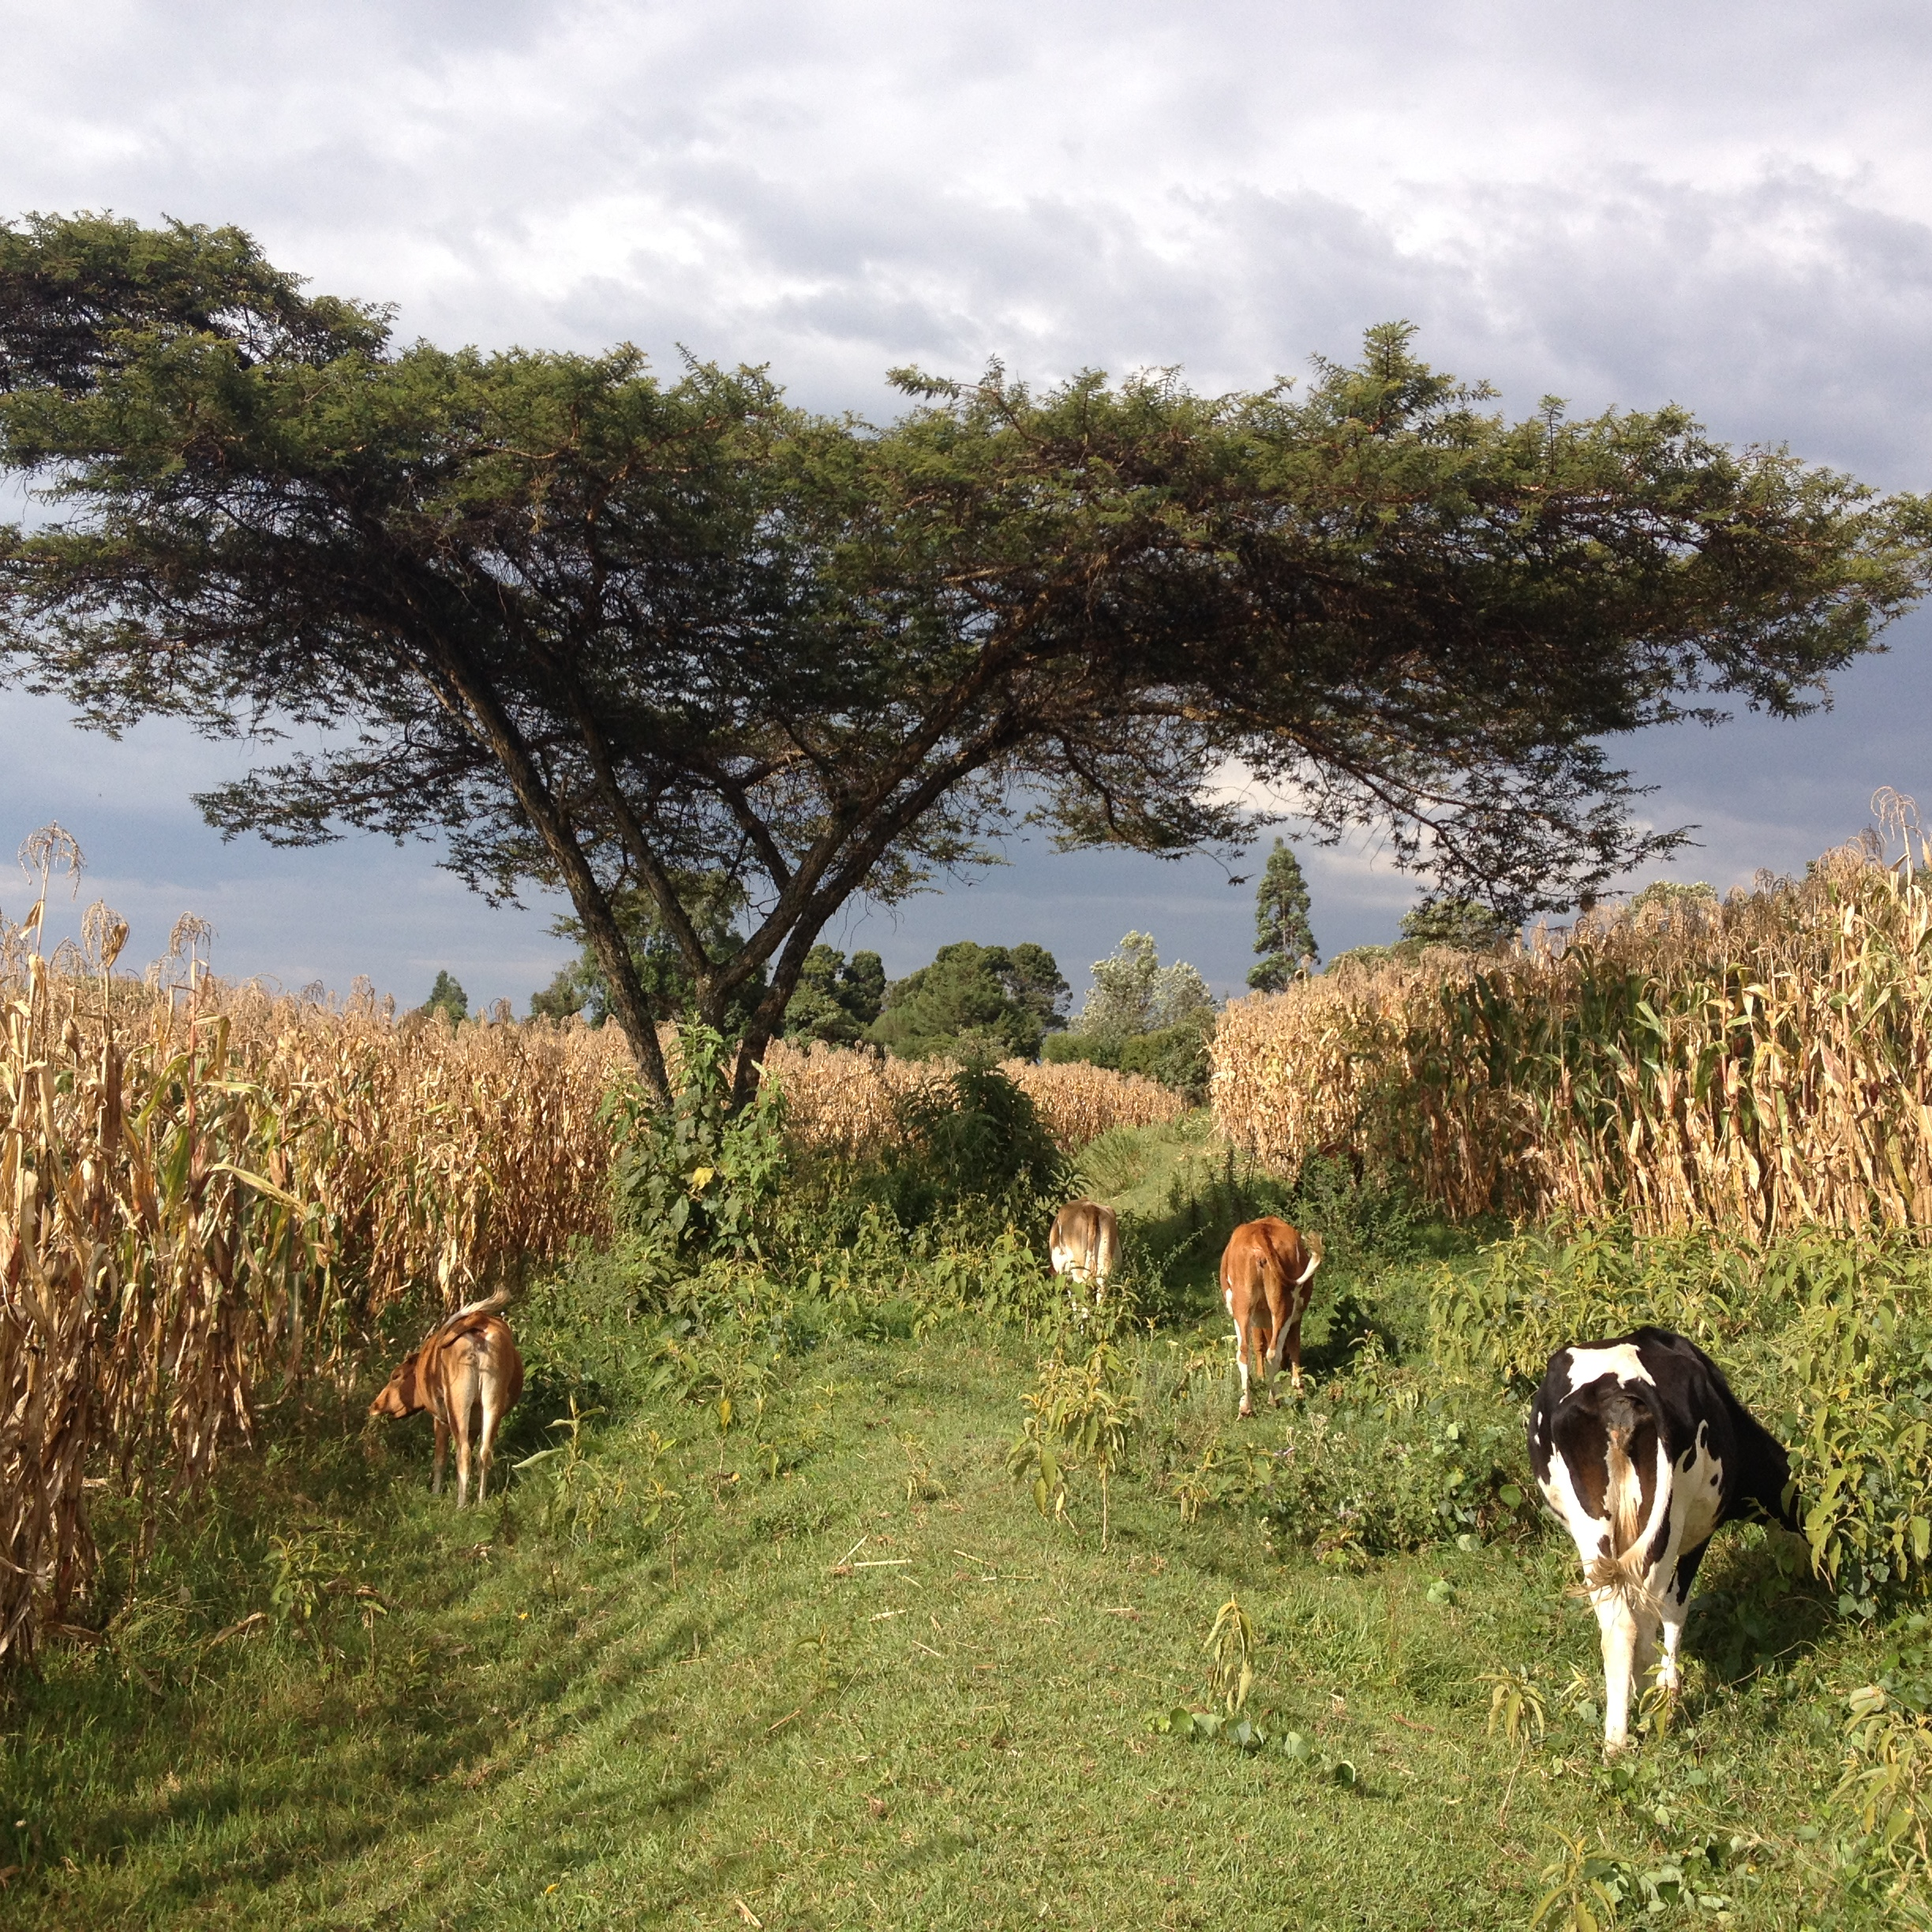
\includegraphics[width=1\textwidth]{cover/NandiMaizeDairy.jpg}
%\end{figure}

\begin{center}
\vspace*{\fill}


\large{Simon Fraval}\\
\end{center}

%%%%%%%%%%%%%%%%%%%%%%%%%%%%%%%%%%%%%%%%%%%%%%%%%%%%%%%%%%%%%%%%
\newpage
\thispagestyle{empty}
\vspace*{\fill}
\begin{tabular}{l}
    \textbf{Thesis committee}                                                                 \\
                                                                                              \\
    \textbf{Promotor:}                                                                        \\
    Prof. Dr I.J.M. de Boer                                                                    \\
    Professor of Animal Production Systems                                                   \\
    Wageningen University \& Research                                                         \\
                                                                                              \\
    \textbf{Co-promotors:}                                                                    \\
    Dr S.J. Oosting                                                                          \\
    Associate professor, Animal Production Systems group                                           \\
    Wageningen University \& Research                                                         \\

    Dr M.T. van Wijk                                                                         \\
    Senior scientist                                                                          \\
    International Livestock Research Institute                                                \\
                                                                                              \\
    \textbf{Other members:}                                                                   \\
    Prof. Dr C. Leeuwis, Wageningen University \& Research                                     \\
    Dr I. Brouwer, Wageningen University \& Research                                     \\
    Dr M.A. Slingerland, Wageningen University \& Research                                \\
    Prof. Dr G. Djurfeldt, Lund University, Sweden                                            \\
                                                                                              \\

    \small{This research was conducted under the auspices of the Graduate School}             \\
    \small{Wageningen Institute of Animal Sciences (WIAS)}                                    \\
\end{tabular}

%%%%%%%%%%%%%%%%%%%%%%%%%%%%%%%%%%%%%%%%%%%%%%%%%%%%%%%%%%%%%%%%
\newpage
\thispagestyle{empty}
\begin{center}
\Huge{\textbf{Food security in rural sub-Saharan Africa}} \\
\large{A household level assessment of crop-livestock systems} \\
\vspace*{1cm}
\Large{Simon Fraval}\\
\normalsize
\vspace*{\fill}
\textbf{Thesis} \\
submitted in fulfilment of the requirements for the degree of doctor\\
at Wageningen University\\
by the authority of the Rector Magnificus,\\
Prof. Dr A.P.J. Mol,\\
in the presence of the\\
Thesis Committee appointed by the Academic Board\\
to be defended in public\\
on Wednesday 10 April 2019\\
at 11 a.m. in the Aula.\\
\end{center}

%%%%%%%%%%%%%%%%%%%%%%%%%%%%%%%%%%%%%%%%%%%%%%%%%%%%%%%%%%%%%%%%%%%
\newpage
\thispagestyle{empty}
\vspace*{\fill}
\begin{flushleft}
\begin{tabular}{l}
    Simon Fraval                                                 \\
    Food security in rural sub-Saharan Africa: A household level assessment of crop-livestock systems                 \\
    \pageref{LastPage} pages.                                    \\
                                                                 \\
    PhD thesis, Wageningen University, Wageningen, the Netherlands (2019)     \\
    With references, with summaries in English and Swahili                  \\
                                                                 \\
    ISBN 978-94-6343-573-4\\
    DOI https://doi.org/10.18174/467544                                            \\
\end{tabular}
\end{flushleft}
%\newpage
%\thispagestyle{empty}
%\begin{flushright}
%\vspace*{\fill}
%\textit{Aan mijn ouders}
%\end{flushright}

\cleardoublepage
\cleardoublepage


\thispagestyle{empty}
%%%%%%%%%%%%%%%%%%%%%%%%%%%%%%%%%%%%%%%%%%%%%%%%%%%%%%%%%%%%%%%%%%

\textbf{Abstract}

\small
Members of rural households in sub-Saharan Africa (SSA) are both vulnerable to the health burdens that stem from food insecurity and central to improving the availability and affordability of wholesome foods. It has been estimated that chronic and hidden hunger can be alleviated by implementing a suite of nutrition-specific interventions at a cost of US\$9.6 billion per annum. This can be accelerated with complementary food system-based interventions. However, such interventions are hampered by a limited understanding of food security status and its associations with rural livelihoods. Therefore, the primary objective of this thesis was to describe, analyse and understand food security in rural landholding households in predominantly mixed crop-livestock agricultural systems of sub-Saharan Africa (SSA). The secondary objective was to improve the methodological basis of household level food security studies.
The rural household multi-indicator survey (RHOMIS) tool was developed to describe and analyse the circumstances of rural households. The RHOMIS tool aims to adhere to the principles of being time-efficient, utilitarian, user-friendly, flexible and reliable. The credibility, consistency and reliability of data collected using three different farm household surveys. The shorter and more targeted survey tool, RHOMIS, performed better in terms of staying within credible bounds. Measurements of maize yields and land area owned were found to be less reliable than other variables. Despite the limitations in data quality, our analysis shows that if the same farm households are followed over time, the sample sizes needed to detect substantial changes are in the order of hundreds of surveys, and not in the thousands.
The RHOMIS tool was then used to quantify changes in livelihoods and food security status in an urban linked, high potential region of Tanzania. Households in the study site adaptively responded to local and national circumstances. Changes in land ownership, livestock-holdings and high value crop production were most likely related to market opportunities and personal circumstances, rather than to direct interventions. Several households made strategic changes by expanding land ownership, planting perennial crops and investing in exotic cattle breeds; many households tactically utilised their land for diversified, mixed crop-livestock production. A central finding of this study is that the complex risk management strategies and market responsiveness demonstrated by the `Rising' clusters are at odds with single focus activities that external organisations tend to promote.
Subsequently, instances of chronic and hidden hunger were analysed in two provinces of Burkina Faso. The results of this study show that in both provinces, the ability to purchase food is what differentiates the more food secure households from their less food secure counterparts. This finding does not detract from the utility of subsistence production -- where consumption of own-farm sourced food catered for between 72\% and 91\% of the annual energy requirements. Further, households were observed to be pursuing market-oriented strategies in combination with production diversification -- likely to reduce risk exposure to climatic or economic shocks.
In a large sample of households across SSA, we found that as many as 40\% of households were classified as chronically hungry in the lean period. Prevalence of micronutrient dietary gaps were high, ranging from 35\% of households to 68\%. Vulnerability to dietary gaps differed by household composition, livelihood characteristics and agro-ecological zone (AEZ). It is the combination of livelihood characteristics and the agro-ecological production potential that drive the availability of food and income. It was found that households fail to purchase food categories that nutritionally complement their own agricultural products. Furthermore, households with a livestock component to their farm were found to have a lower prevalence of chronic and hidden hunger.
In extended analyses, the gender of household head and stage of life were found to be associated with the number of household inhabitants and thus influence nutritional requirements and food security status throughout the year. The high prevalence of food insecurity, the complexity of associations and the failure to nutritionally complement own-production with purchases have implications for developing effective interventions. Programs can be designed as `packages' of agricultural and non-agricultural interventions to maximise adoption and maximise the positive impact on food and nutrition security throughout the year.

\normalsize
%\vspace*{\fill}


\cleardoublepage

\addtocontents{toc}{\protect\setcounter{tocdepth}{-1}} %Exclude reference to the TOC. Last answer to this post https://tex.stackexchange.com/questions/10943/how-to-remove-the-self-reference-of-the-toc-from-the-toc
\tableofcontents
\addtocontents{toc}{\protect\setcounter{tocdepth}{0}} %set depth to the levels of heading that you want to display. 3 = sub-sub headings included

\pagenumbering{arabic} \setcounter{page}{1} %Page numbering starts from main matter


%% Main Chapters
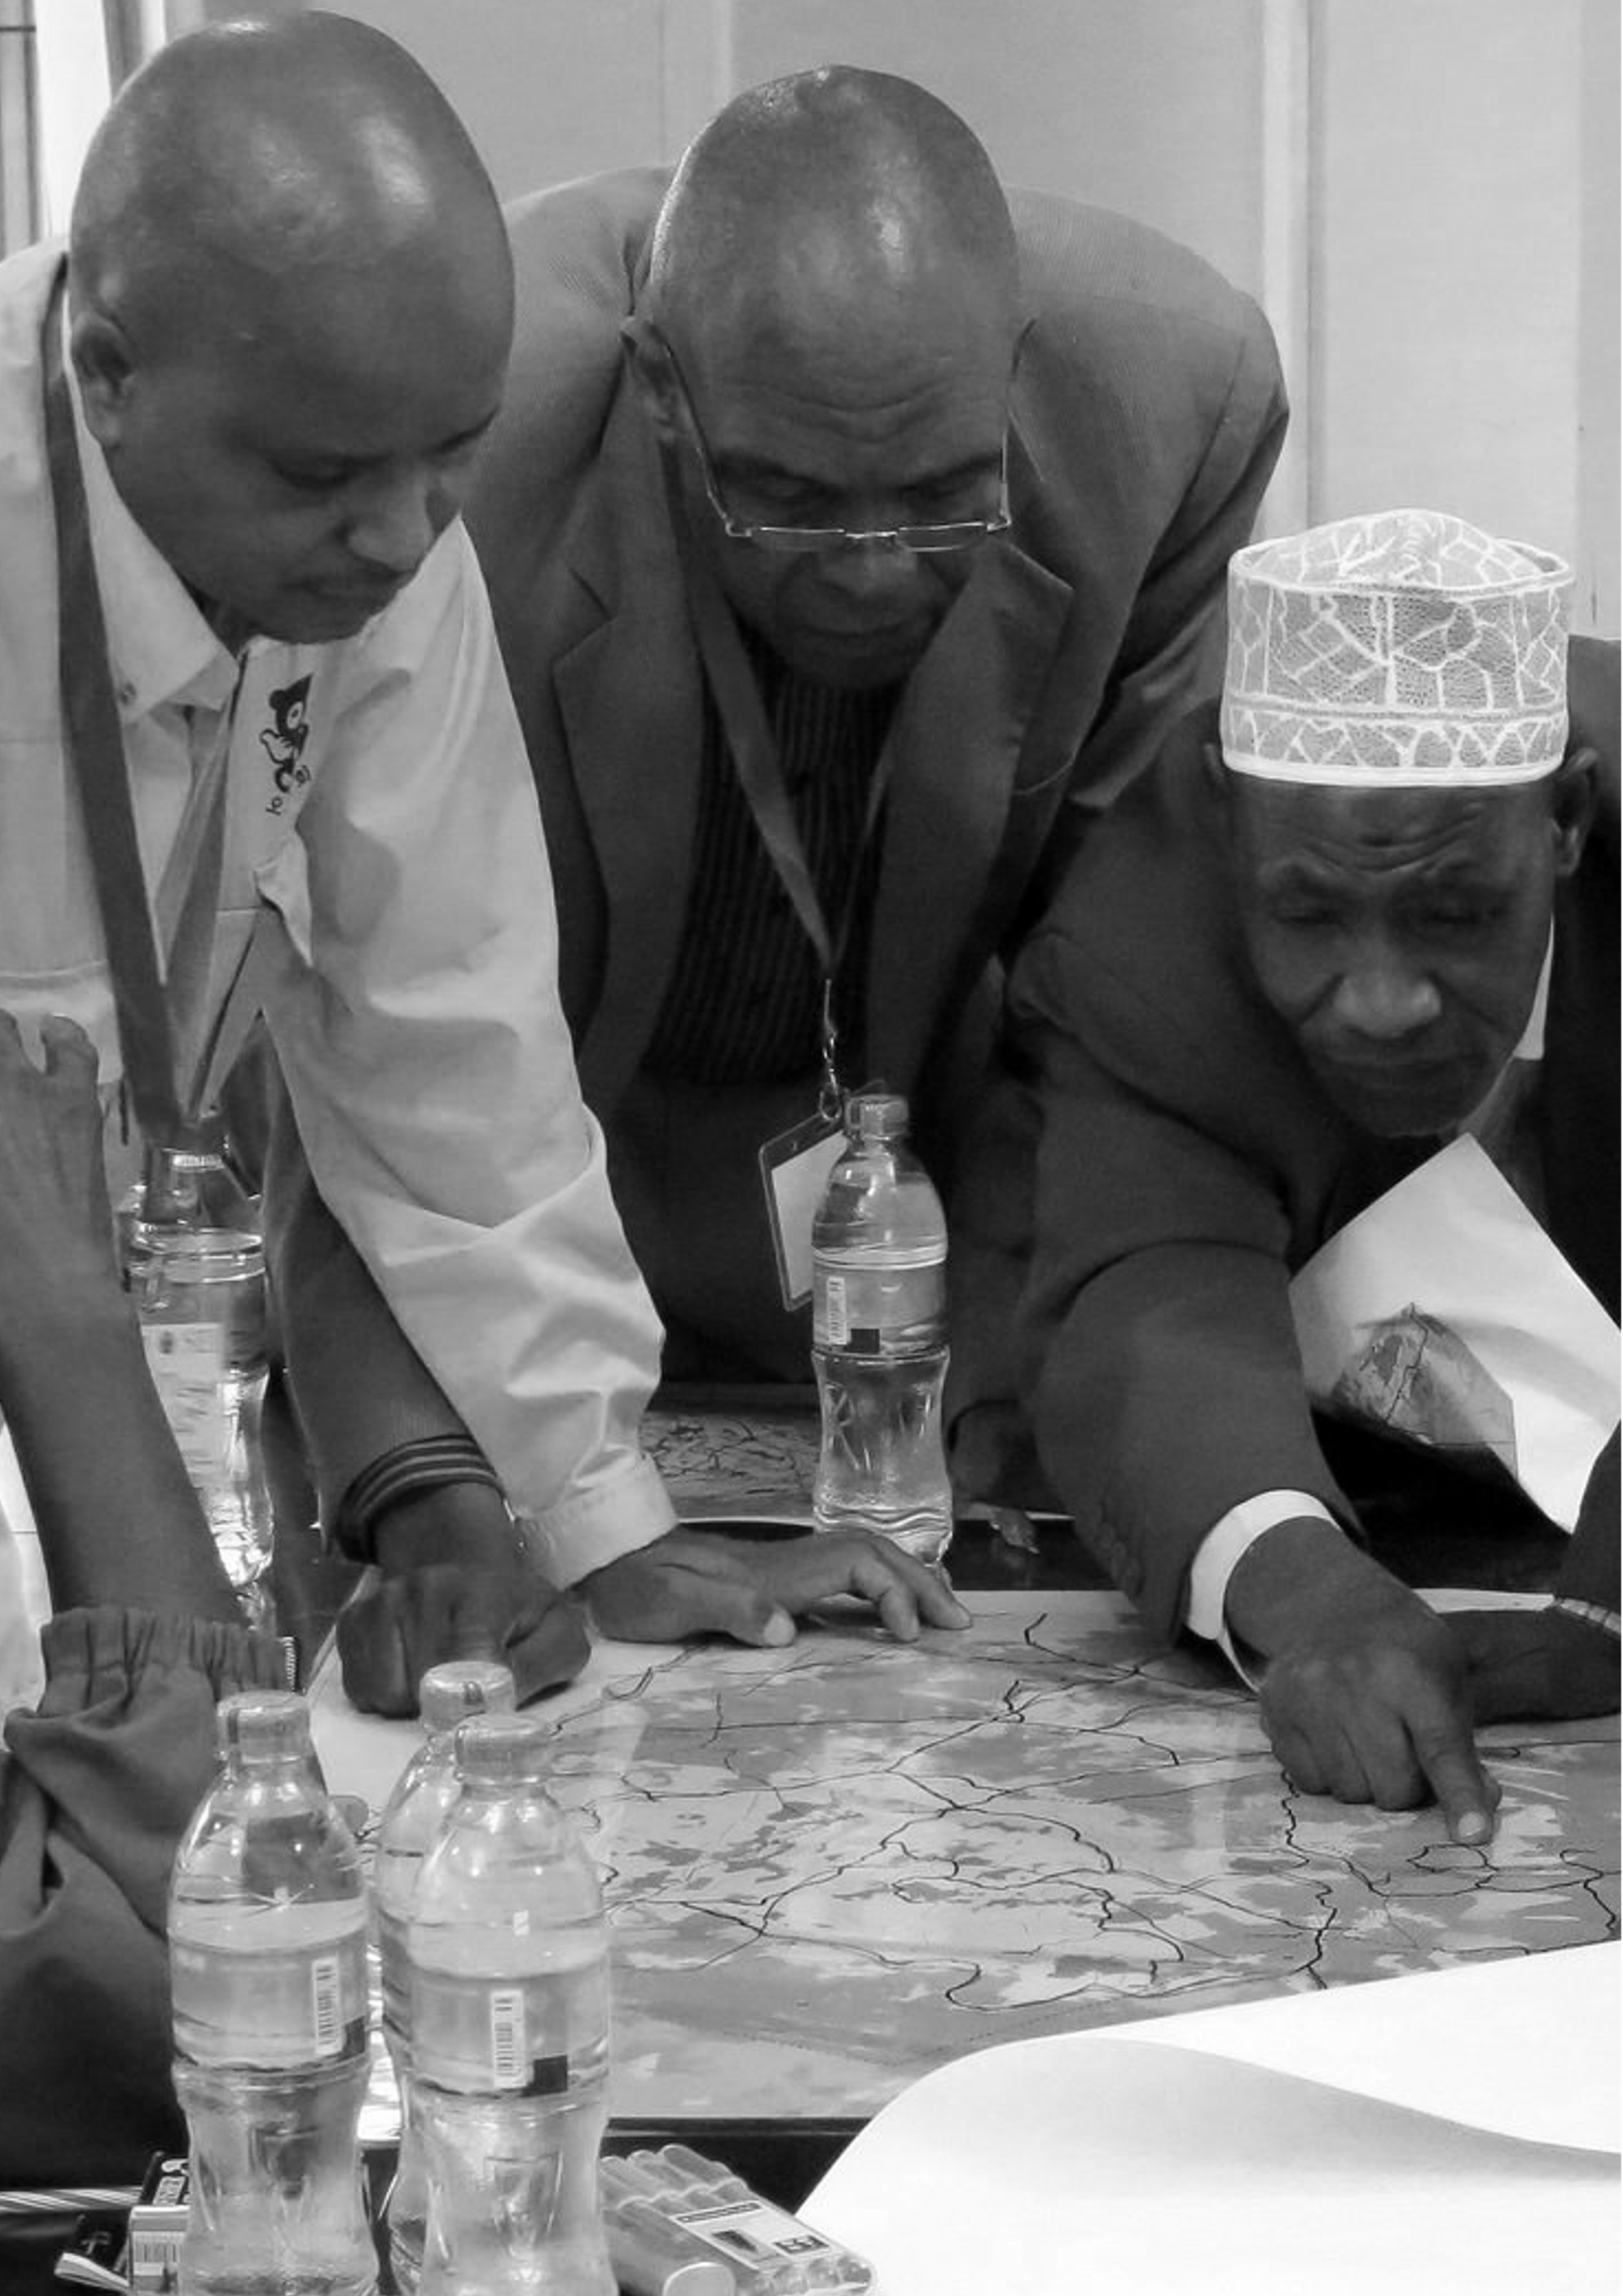
\includepdf{ChapterPics/Ch1CLEANED.png}
\mainmatter


\setcounter{page}{1}
\chapter[General introduction]{General introduction}
\chaptermark{General introduction} %Title for running head
\label{cha:Chapter1}
\vspace*{\fill}


\newpage

\section{Background}

Malnutrition affects the quality of life for a substantial portion of the human population (\citealp{GBD2016RiskFactorsCollaborators2017}). Chronic undernourishment, micronutrient deficiencies and obesity increasingly co-exist within the same communities – forming a triple burden of malnutrition (\citealp{May2018}). The incidence of adverse health effects due to chronic undernourishment and micronutrient deficiencies are substantially higher in sub-Saharan Africa (SSA) compared to the rest of the world (\citealp{Godecke2018, GBD2016RiskFactorsCollaborators2017}). In addition, the rural population in SSA bear a disproportionately large share of the individual and societal implications following such nutritional gaps when compared to urban communities (\citealp{Headey2018a, Green2016}).

This thesis focuses on the food security status of rural landholding households in SSA. Members of rural landholding households are both vulnerable to the health burdens that stem from food insecurity and central to improving the availability and affordability of a diversity of wholesome foods for both rural and urban markets (\citealp{Fanzo2018}).

\subsection{Food security}

Food security forms the basis of human well-being. By definition, food security exists ``when all people, at all times, have physical and economic access to sufficient safe and nutritious food that meets their dietary needs and food preferences for an active and healthy life'' (\citealp[p.~1]{FAO2008}). This definition of food security encompasses four dimensions, namely: food availability, food access, food utilisation and stability (\citealp{FAO2008}). Food access refers to an ability to source or acquire food using available resources (\citealp{Maxwell1992}). Having the ability to access food does not necessarily result in consumption -- this distinction is made in the food utilisation dimension of food security. Food utilisation can be diminished by competing livelihood goals or decisions related to the distribution of food. Furthermore, the sufficiency of food utilisation depends on an individual's nutritional requirements which can vary depending on age, gender, exertion and health. Stability refers to how food access and food utilisation are experienced over time. Food security only exists when each individual is able to consume sufficient, safe and nutritious foods at all times -- throughout the weeks, months and years. People, however, cannot access or utilise food when it is not available. This makes the functioning of agricultural systems central to food security.

\subsection{Food availability and agricultural systems}

Agricultural systems in SSA are diverse and dynamic -- driven by numerous exogenous (e.g. agro-ecological conditions, soil fertility, urban proximity and local policies) and endogenous (i.e. related to the livelihoods of the rural population) factors. Agricultural systems can be classified in terms of their crop and livestock production mix, dependence on precipitation, agronomic practices, animal husbandry practices, market orientation, scale, or capital intensity (\citealp{Garrity2012, Sere1996}).

\subsubsection{Overview of agricultural systems in SSA}

The production potential of agricultural systems in SSA are generally determined by the annual and seasonal rainfall quantity (\citealp{VanOort2016}). This dependence means that agro-ecological zones (AEZs) play a significant role in determining land use, both for the vast rangeland areas and the two million hectares of cultivated land in SSA. Rangelands are typically located in arid (length of growing period (LGP) {\textless} 75 days) and semi-arid (LGP 75 -- 180 days) lands (ASALs). Nomadic and transhumance communities utilise these rangelands as a feed resource for small and large ruminants (\citealp{Sere1996}). Sedentary farmers also occupy ASALs, in instances where soil conditions, water availability and market conditions allow. These sedentary farmers, however, are generally limited in the range of crops cultivated (\citealp{USAID2012, Little2001}). In contrast, a wide array of staple and cash crops can be cultivated under rainfed conditions in sub-humid (LGP 181-270 days) and humid (LGP {\textgreater} 270 days) AEZs. Warm sub-humid zones are suited to cereals, legumes, bananas, oilseeds, sugarcane, forages, sisal and tree-nuts (e.g. western Kenya and large areas of Tanzania; \citealp{USAID2012, USAID2009}). Cool sub-humid and humid zones (highland regions) are suited to cereals, legumes, bananas, root crops, coffee, tea, cacao, vegetables, fruits and forages. Mixed crop-livestock systems are common across AEZs and geographical regions (\citealp{B.D.PerryT.F.Randolph2002}). These systems are defined as those that feed 10\% of crop residue dry matter to livestock or earn at least 10\% of farm income from crop production (\citealp{Sere1996}).

\subsubsection{Food availability: current status and future trends}

Despite this wide-ranging diversity of agricultural production systems in SSA, the availability of energy-dense and nutrient-rich foods is worryingly strained. On balance, one-quarter of the one billion people in SSA are suffering from insufficient food energy supply (\citealp{FAO2018}). In addition, the availability of micronutrients falls short of requirements -- resulting in what is termed `hidden hunger' (\citealp{Joy2014, Kumssa2015, Harika2017}). It is estimated, for example, that 50\% of the African population is at risk of calcium deficiency, 40\% of zinc deficiency, 28\% of selenium deficiency and 19\% of iodine deficiency (\citealp{Joy2014}). These supply shortfalls are compounded by barriers to access and utilisation. The insufficient availability of energy dense and diverse foods is forecast to worsen in the medium to long term as demand for animal source foods exceeds supply, yields stagnate or decline, and the homogeneity of crop species increases (\citealp{Enahoro2018, VanOort2016, Pingali2015}). Medium and small-scale farms serve differing functions in SSA food systems. Regardless of farm scale, however, yield gaps will need to be closed for energy dense and micronutrient rich foods.

In SSA, medium scale farms (2 - 20 ha) produce 50\% of the volume of each food category (e.g. cereals, root crops, vegetables and livestock; \citealp{Herrero2017}). Smallholder farmers (${\leq}$ 2 ha) also contribute substantially to food availability (\citealp{Samberg2016}) as they allocate a greater proportion of their land to food crops, including a greater diversity of food crops compared to medium scale farms (\citealp{Ricciardi2018}). In total, smallholder farmers produce 25\% of the volume of most food commodities (\citealp{Herrero2017}), while using 40\% of agricultural land (based on an assessment of 9 countries in SSA by \citealp{Lowder201616}).

There are substantial gaps between actual and potential yields in SSA farming communities, both for crops and livestock. Thus, total food availability is far below the potential. It has been estimated that livestock productivity can almost double and crop productivity can more than double (\citealp{Henderson2016106}). Existing yield gaps are common due to climatic shocks (\citealp{Gebrechorkos2018}), pests and diseases (\citealp{Biber-freudenberger2016}), long-term depletion of soil resources (\citealp{Tittonell2013}), and resource constraints of the farmers (both for inputs and capital expenditure). By closing the crop yield gaps alone, 95\% of SSA nations could meet their current human metabolic energy needs (\citealp{Luan2018}).

Meeting the full dietary needs of SSA populations will require a diversity of foods to be readily available (i.e. more diverse than energy-dense foods alone). The increasing homogeneity of species cultivated is evident globally (\citealp{Khoury2014}). African nations are no exception, where traditional lower yielding grains such as tef, millets and sorghum are gradually being substituted with maize, traditional vegetables replaced with market vegetables, and livestock genetic resources have narrowed. This increased homogeneity may be positive for overall kilocalorie availability, but this benefit has trade-offs with the need to have access to nutritionally diverse and culturally relevant food for the population (\citealp{Schipanski2016, Pingali2015, Remans2014, Popkin2001}). This is evident in the substantial supply deficiency of fruits and vegetables in African nations -- ranging from a shortage of 12\% (Ghana and Camaroon) to 90\% (Burkina Faso; \citealp{Siegel2014}).

\subsection{Food access, utilisation and stability in the context of rural livelihoods}

Agriculture generates between 20\% and 50\% of gross domestic product (GDP) across SSA (\citealp{Proctor2014}). In rural SSA, 92\% of households are engaged in farming to some extent and 52\% are specialised in farming -- with farming in accounting for approximately 69\% of rural incomes (\citealp{Davis2017}). Rural landholding households, therefore, a) provide livelihood opportunities for rural landless households, b) are vital contributors to domestic food availability, from local to national level, and c) depend on agriculture to meet their own needs for a stable supply of safe and nutritious food. Meeting nutritional needs, however, is only one goal of many. Instead, individuals within households strategically and adaptively make use of various capabilities to increase income, to maximise well-being, to reduce vulnerabilities and to reinvest in productive assets (including the natural resource base; \citealp{Ashley1999, Farrington1999, Scoones1998}). To define this use of capabilities more formally, `livelihoods' are ``the control an individual, family, or other social group has over an income and/or a package of sources that can be used or changed to maintain a living'' (\citealp[p.~9]{Blaikie1994}). Capabilities stem from five `livelihood assets' termed: financial, human, natural, physical and social capital (\citealp{Farrington1999}). These capabilities in rural SSA are often pooled at the household level.


\subsubsection{Households in SSA}

A `household' is an amorphous concept that defines an economic unit above the individual (\citealp{Randall2015}). A household has been defined as a group of people ``who combine to occupy the whole or part of a housing unit and to provide themselves with food or other essentials for living'' (\citealp[p.~74]{UnitedNations1959}) -- where there may be some variability in co-habitation and frequency of meal sharing. In rural SSA, a household can be composed of family members (including extended), non-family dependents and workers. The composition of a household is influenced by relationship status, marital arrangements, life stage, fertility, family planning, available resources and health circumstances. There are a large number of possible household compositions, for example three generations of family, single parents and families where one parent works away from home (\citealp{Randall2015}). The composition of a household has a significant influence on livelihood assets and goals.

The use of livelihood assets and the prioritisation of livelihood goals (e.g. food security or education) can be a strategic or an adaptive process -- mediated by complex intra-household dynamics (\citealp{Kazianga2017, Galie2015}). The gendered dimensions of decision making, labour allocation and control of resources are highly context specific (\citealp{Doss2013}). In rural SSA, patriarchal norms prevail, and women tend to have higher labour burdens, less decision-making power and less control of financial resources (\citealp{Sofa2011}). Land use decisions and control of financial resources have a substantial bearing on food security (\citealp{Dzanku2019, Price2018, AnderssonDjurfeldt2018b}). There is a tendency for female-headed households in SSA to cultivate a greater proportion of food crops than their male-headed counterparts who tend to favour cash crops (\citealp{tibesigwa2018contribution}). In general, improved `status' of women in households is positively associated with nutritional outcomes of the household and children more specifically (\citealp{Bhandari2017, doi:10.1093/ajcn/nqy001, JIN201416}). Land use decisions, off-farm income opportunities and intra-household dynamics are central to the livelihoods of rural landholders, and their food security.

\subsubsection{Land use decisions and land size trends}

Land and livestock ownership are important enabling assets for rural households. Land provides production opportunities and livestock provide a means of diversifying income sources, buffering exposure to climatic and market shocks, draught power, recycling nutrients and storing wealth (\citealp{Thornton2015, Swanepoel2010, Moll2005, McIntire1992}). Exogenous factors (e.g. agro-ecological conditions, soil fertility, urban proximity and local policies) determine production possibilities and potential returns. Agricultural production decisions are then made based on exogenous factors, livelihood goals, intra-household dynamics and livelihood assets. Specifically, decisions may be made on composition (crop and livestock species), area allocated, and practices adopted. In tandem, households decide on whether to `value-add' (e.g. by milling grain or processing milk), what proportion to retain for home consumption, and which market avenues to pursue. Land use decisions are also significantly influenced by land sizes.

Small land sizes limit a household's capacity to produce enough food and income to meet their basic needs. In many cultures of SSA, parents sub-divide land amongst their children. This practice has progressed to the point where smallholder farms are no longer economically viable (\citealp{Lowder201616, Jayne2014}). The size of smallholder farms has now stagnated, and medium scale farmers are managing an increasing share of total farm area (\citealp{AnderssonDjurfeldt2018a, Jayne2016}). In a study of four African nations, \citet{Jayne2016} found that half of the medium scale farmers purchased land later in life with capital raised from off-farm income. These medium scale farms are characterised as being highly commercialised with substantial influence on government policy. On the other hand, smaller farm sizes have resulted in prioritisation of short-term needs, often at the expense of soil quality -- manifested as shortened fallow periods, minimal inputs and limited utilisation of other soil conservation practices (\citealp{Tittonell2013}). Additionally, instances of crop-livestock integration tend to decrease as farm sizes become too small to cater for the needs of their livestock (\citealp{Thornton2015}).

\subsubsection{Diversified income sources: off-farm}

Off-farm income can be earned through entrepreneurial activities, seasonal informal employment and formal employment -- earned in the household or sent back as remittances. Diversifying income sources in this way buffers exposure to climatic and market shocks (\citealp{Silvestri2015}), increases net incomes (\citealp{AnderssonDjurfeldt2018}) and may provide a means to access credit for the farm business. There are, however, limited opportunities to earn off-farm income, where the most readily available informal farm labour options offer low returns (\citealp{Jayne2014}), and wealthier and more educated households have a greater capacity to gain employment or invest in a non-farm business (\citealp{Davis2010, Haggblade2010, Reardon1992}). This constrained labour market is forecasted to continue as population density increases -- particularly for poorer, less educated households (\citealp{FAO2015a, deBrauw201433}).

\subsubsection{Temporal dynamics of livelihoods}

Household composition, enabling assets and off-farm income opportunities are by no means static. Livelihoods change over time
through strategic efforts and adaptive responses to shocks and opportunities. For example, households can strategically invest in irrigation (\citealp{Nakawuka2017}), or adaptively respond to drought (\citealp{Ulrich2012241}). The temporal dynamics of livelihoods highlights the point that short-term needs are met in a broader context of long-term resilience. Specifically, the depletion of livelihood assets (such as soil fertility) to meet short-term needs can increase long-term risk exposure to shocks and reduce capacity to capitalise on opportunities. As such, livelihood strategies have been classified as those that are `Hanging-in' (trying to maintain a livelihood), `Stepping-up' (improving livelihoods by expanding an activity) or `Stepping-out' (using asset base to move into new livelihood activities; \citealp{Dorward2009}) and `Dropping-out' (unwillingly leaving agriculture; \citealp{Valbuena20151395}).

\subsection{Monitoring nutrition, diets and food security}

Improving livelihoods does not necessarily improve human nutrition. As such, human nutrition and food security need to be monitored over time to inform policies and interventions. The constituents of human nutrition include macronutrients (carbohydrates, protein, fat and fibre), micronutrients (vitamins and minerals) and water. Nutritional requirements will depend on age, gender, physical activity, health status, physiological status (e.g. pregnant), and genetics. The absorption of nutrients delivered to the gastrointestinal tract will depend on diet composition, health status and physiological status. Dysfunction and disease can arise due to unbalanced and deficient diets. Food insecurity, in this broader context, refers to deficient diets due to food access and utilisation constraints. To emphasise the centrality of human nutrition in food security, this thesis at times uses the term `food and nutrition security' instead of food security.

Nutritional status can be most directly monitored through biomarkers and anthropometrics (e.g. body mass index or height for age). Monitoring diets, however, is less invasive and less costly. Therefore, monitoring national and sub-population diets has provided a foundation for preventative health strategies in many countries. Individual and household diets have traditionally been monitored using 24-hour dietary recall (24hR), food frequency questionnaires (FFQ) and, to a lesser extent, longitudinal food records (\citealp{Micha2018, Vila-real2018}). These methods are highly heterogeneous with various modes of data collection, food classification systems, food volume quantification protocols and professional capacity requirements (\citealp{Micha2018, Keyzer2015}). The 24hR and FFQ methods can be self-administered or conducted by an interview with pen-and-paper, computer-aided or over the telephone. The 24hR method can be applied multiple times, enumerating all food, beverages and dietary supplements consumed for the previous 24 hours -- where a minimum of three observations is recommended (\citealp{Ma2009}). The FFQ method can elicit information on the frequency of tens or hundreds of items consumed over one week or longer. Quantifying food volumes is one of the most challenging aspects of these methods, where various physical, visual and technical aides are in use. Interviews are generally conducted by nutritionists, dietitians or enumerators familiar with local diets (\citealp{Keyzer2015}). Policy makers and researchers have also used 24hR and FFQ to study SSA populations.

In East and West Africa, 24hR were predominantly applied for epidemiological studies, nutritional monitoring or impact assessments of interventions (\citealp{Pisa2017}). In contrast, FFQs were used to assess food habits and nutrient intakes. These various applications were highly heterogeneous in duration, number of recalls (24hR), recall period (FFQ), validation (e.g. only 3 out of 9 24hR programs in West Africa and no 24hR programs in East Africa were validated against biomarkers) and reliability assessments (see \citealp[p.~56]{Pisa2017}; \citealp[Tables 2 \& 3]{Vila-real2018}). All national programs assessed in \citet{Pisa2017} conducted interviews by pen-and-paper.

In SSA, the relatively high cost of anthropometric, biomarker and diet surveillance has necessitated coarser estimates of food security status -- initially using existing data. At a macro-level, food balance sheets (FBS) provide an estimate of food availability per capita based on production, transformation, trade and population requirements (\citealp{Micha2018}). At a micro-level, household consumption and expenditure surveys (HCES) -- primarily designed to calculate consumer price indices (CPI) -- have been utilised as a means of assessing dietary adequacy of purchased foods (\citealp{Micha2018, Burchi2016, Carletto2013}).

More recently, proxies have been developed to enable frequent and wide-scale measurement (\citealp{Pisa2017, Keyzer2015}). Two prominent indicators are: household food security of access and diet diversity. The household food security of access indicator is based on a series of nine questions of increasing severity, from worry about food availability to missing an entire day of food due to availability. For example, severe food insecurity (of access) is defined as regularly eating smaller meals than desired, regularly eating fewer meals than desired or worse. Diet diversity indicators are based on a count of food categories consumed. There are a range of diet diversity indicators, varying by the aggregation and inclusion of food categories. Food insecurity of access and diet diversity metrics have been assessed against traditional anthropometric status and adequacy ratios and have emerged as valid proxies (evident in \citealp{McDonald2015, Rah2010, Saha2009, Coates2007, Savy2005, Steyn2006, Arimond2004, Torheim2004}).

\section{Knowledge gaps and objectives}

The global community has committed itself to reverse trends in food insecurity, here denoting the two concepts of chronic and hidden hunger (\citealp{FAO2018}). It has been estimated that much of the chronic and hidden hunger that we see today can be alleviated by implementing a suite of interventions at a cost of US\$9.6 billion per annum (\citealp{Bhutta2013}). Figure 1.1 outlines three strategies that can accelerate the effectiveness of such an investment -- including increasing supply, adding nutrition value and increasing demand. However, such strategies are hampered by a limited understanding of: a) the prevalence of food insecurity b) the spatial distribution of food insecurity, and c) the associations between food insecurity and livelihoods -- the outcomes and impact section of Figure 1.1. These three knowledge gaps are summarised in this section.

\begin{figure}
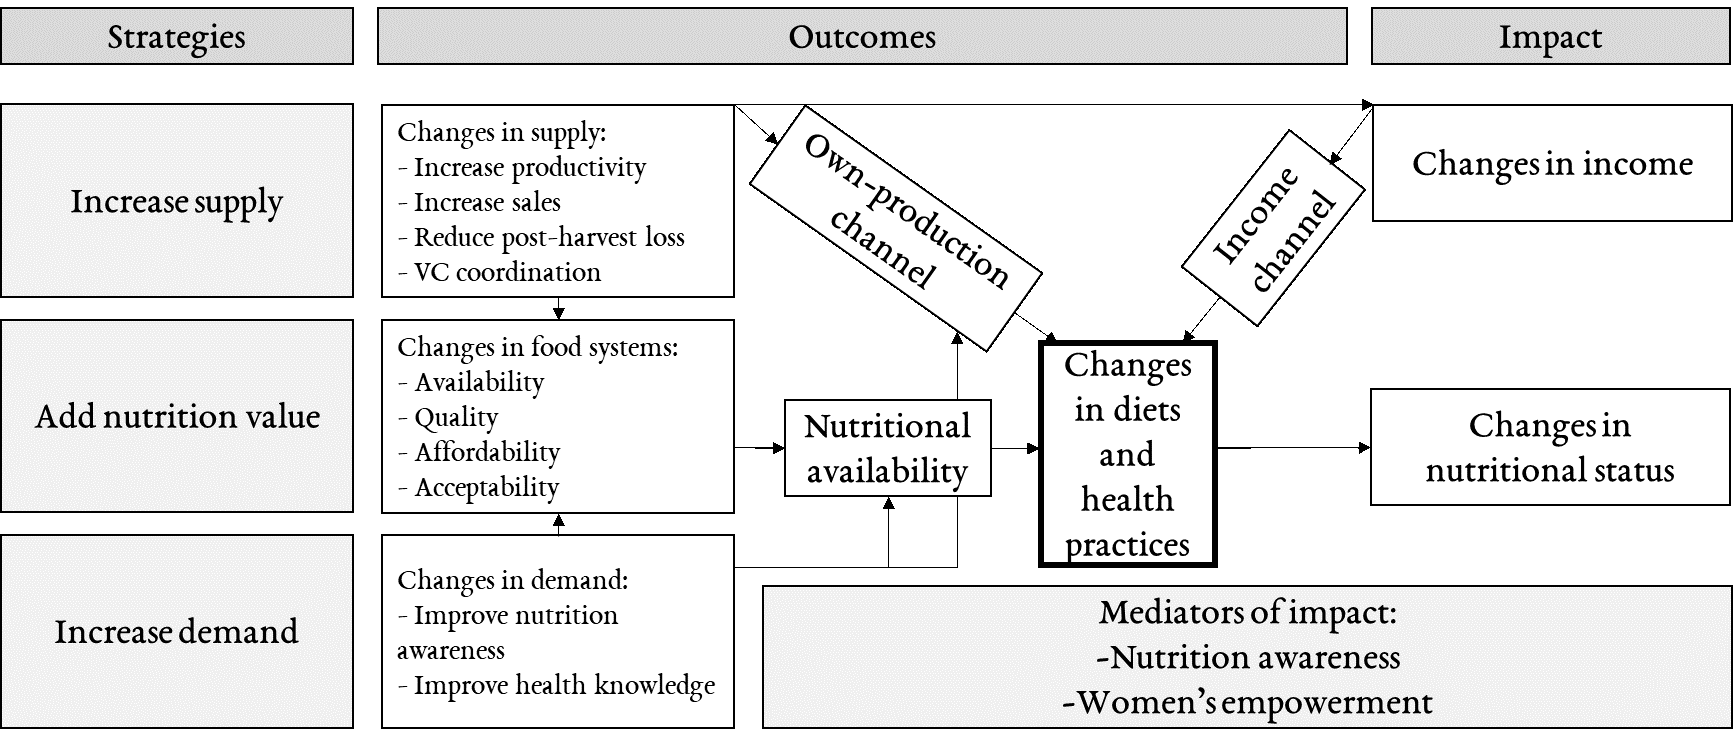
\includegraphics[width=1\textwidth]{figs_07/IFAD_frameworkv2.png}
  \captionsetup{singlelinecheck = off, justification=justified} %left justify caption
  \caption{Impact pathways of food system-based nutrition-specific and nutrition-sensitive interventions}
  \label{fig:01_1}
  %\small
  %\raggedright
  \vspace*{-3mm}
  \caption*{VC = value-chain \\
 	(Reproduced with permission from \citealp{DeLaPena2018})}

\end{figure}

\subsection{The prevalence and spatial distribution of food insecurity}
Our best estimates of chronic and hidden hunger globally are based on FBS. These estimates provide vital insights into the deficiencies of global and regional food supplies. FBS for energy are compiled annually -- providing insights into trends and macro level associations (such as conflict and climate change; \citealp{FAO2018}). Assessments of hidden hunger are less common (\citealp{Kumssa2015, Joy2014}). Estimates from FBS are limited by low-quality data, simplifying assumptions, under-representation of informal trade and subsistence food, and assumptions of equal access to food supplies (\citealp{Micha2018}). The accuracy of FBS has been assessed against nationally representative household microdata -- generally finding poor agreement, with some level of convergence (\citealp{Desiere2018, Gobbo2015, Dowler1985278}). The assumption that each individual in the population has equal access to food and utilises what they need, however, under-represents food insecurity and masks the spatial distribution of food insecurity (\citealp{Micha2018}).

In contrast to FBS, the household level assessments (24hR, FFQ and food (in)security proxies) can provide more accurate and spatially explicit prevalence estimates of food insecurity. The food insecurity experience scale (FIES), for example, has been implemented in 140 countries with samples of more than 1,000 respondents per country (\citealp{FAO2018}). However, as the FIES indicator only represents food insecurity of access, other aspects of food security such as diet diversity and nutrient adequacy do not have the same global scale and frequency of application. These knowledge gaps related to the prevalence and spatial distribution of food insecurity also have a bearing on our knowledge of the associations between food security and livelihoods.

\subsection{Associations between food security and rural livelihoods}
The research community has been exploring the associations between food insecurity and rural livelihoods on national and sub-national scales. The emerging areas of investigation have centred on the role that agricultural production (subsistence and market-orientated) and off-farm income plays in improving food insecurity of access, diet diversity and nutrient adequacy ratios. Income, and thus purchased foods has been found to be highly associated with dietary diversity in a majority of these studies, whereas food from subsistence production, while also significant, has had a limited association with dietary diversity (\citealp{Bellon2016, Koppmair2017325, Luckett20152479, Sibhatu201510657, Snapp2015, Dillon2014}). In comparison, \citet{Jones2016} and \citet{MKaibi2015} emphasised the positive relationship farm production has with nutrition metrics. In the most geographically diverse study to date, the role of farm production on nutrition was found to be of varying importance depending on market opportunities (\citealp{Sibhatu201510657}). These findings, however, are dependent on food security at the time of survey and, as mentioned previously, have a limited geographical scope -- limiting cross-site comparisons and more generalisable inference.

The limitations in performing cross-site comparisons are -- in part -- due to a lack of coordination between organisations. This lack of coordination has resulted in a ``multiplicity of survey instruments collecting information on various dimensions of food and nutrition security'' (\citealp[p.~30]{Carletto2013}). The impetus to harmonise rural household microdata comes as nationally representative studies have been constrained in uptake and frequency of implementation (\citealp{Desiere2018, Carletto2013}). Progress has been made to overcome this research gap over the past decade (e.g. \citealp{Carletto2009, Herrero2007}). A harmonised data collection effort, however, has still not yet been realised. \citet[p.39]{Carletto2013} suggest that this harmonisation can be developed over time, with a ``combination of short-term fixes and long-term methodological advancements''.


\subsection{Objectives}

The primary objective of this thesis was to characterise food and nutrition security in rural landholding households in predominantly mixed crop-livestock agricultural systems of sub-Saharan Africa (SSA). Characterisation in this respect refers to describing the multiple facets of food and nutrition security, and identifying their associations with livelihoods. The related hypothesis is that variation in livelihoods between communities are strongly influenced by agro-climatic conditions, market opportunities and productive assets. It is also hypothesised that nutrition-related outcomes to a certain extent are determined by the livelihood characteristics present in a community. Understanding the context-specific relationships between livelihoods and food security will be essential to inform nutrition-specific (e.g. supplementation \& fortification) and nutrition-sensitive interventions (e.g. agricultural interventions that indirectly improve nutrition).

The secondary objective was to improve the methodological basis of household level food security studies. The related hypotheses to this objective are: 1) existing rural household surveys can be improved upon based on critical evaluation of reliability and credibility, 2) the quantification of food and nutrition security can be integrated with rural household surveys to capture conditions throughout the year, independent of survey timing, 3) research efforts of multiple organisations can be harmonised by providing an effective tool (survey).


\section{Outline of the thesis}

This thesis proceeds by introducing the `rural household multi-indicator survey' -- RHOMIS. Chapter 2 provides a summary of the design principles, indicators and pilot applications of RHOMIS. The data quality associated with rural household surveys is then critically evaluated in Chapter 3. The results of Chapter 3 then have a bearing on the analysis and inference of the three proceeding observational chapters. Chapter 4 provides an assessment of the livelihoods and food security status of households in an urban linked, high potential region of Tanzania over a three-year period. Chapter 5 provides an assessment of the pathways to food security in northern Burkina Faso, with a specific focus on the consumption of home-produced food versus purchased food. Chapter 6 provides an assessment of dietary gaps across multiple locations in sub-Saharan Africa. Chapter 7 then provides a synthesis of findings in this thesis, drawing together common themes and identifying areas for future research. Figure 1.2 provides a diagrammatic overview of this thesis.

\begin{figure}
    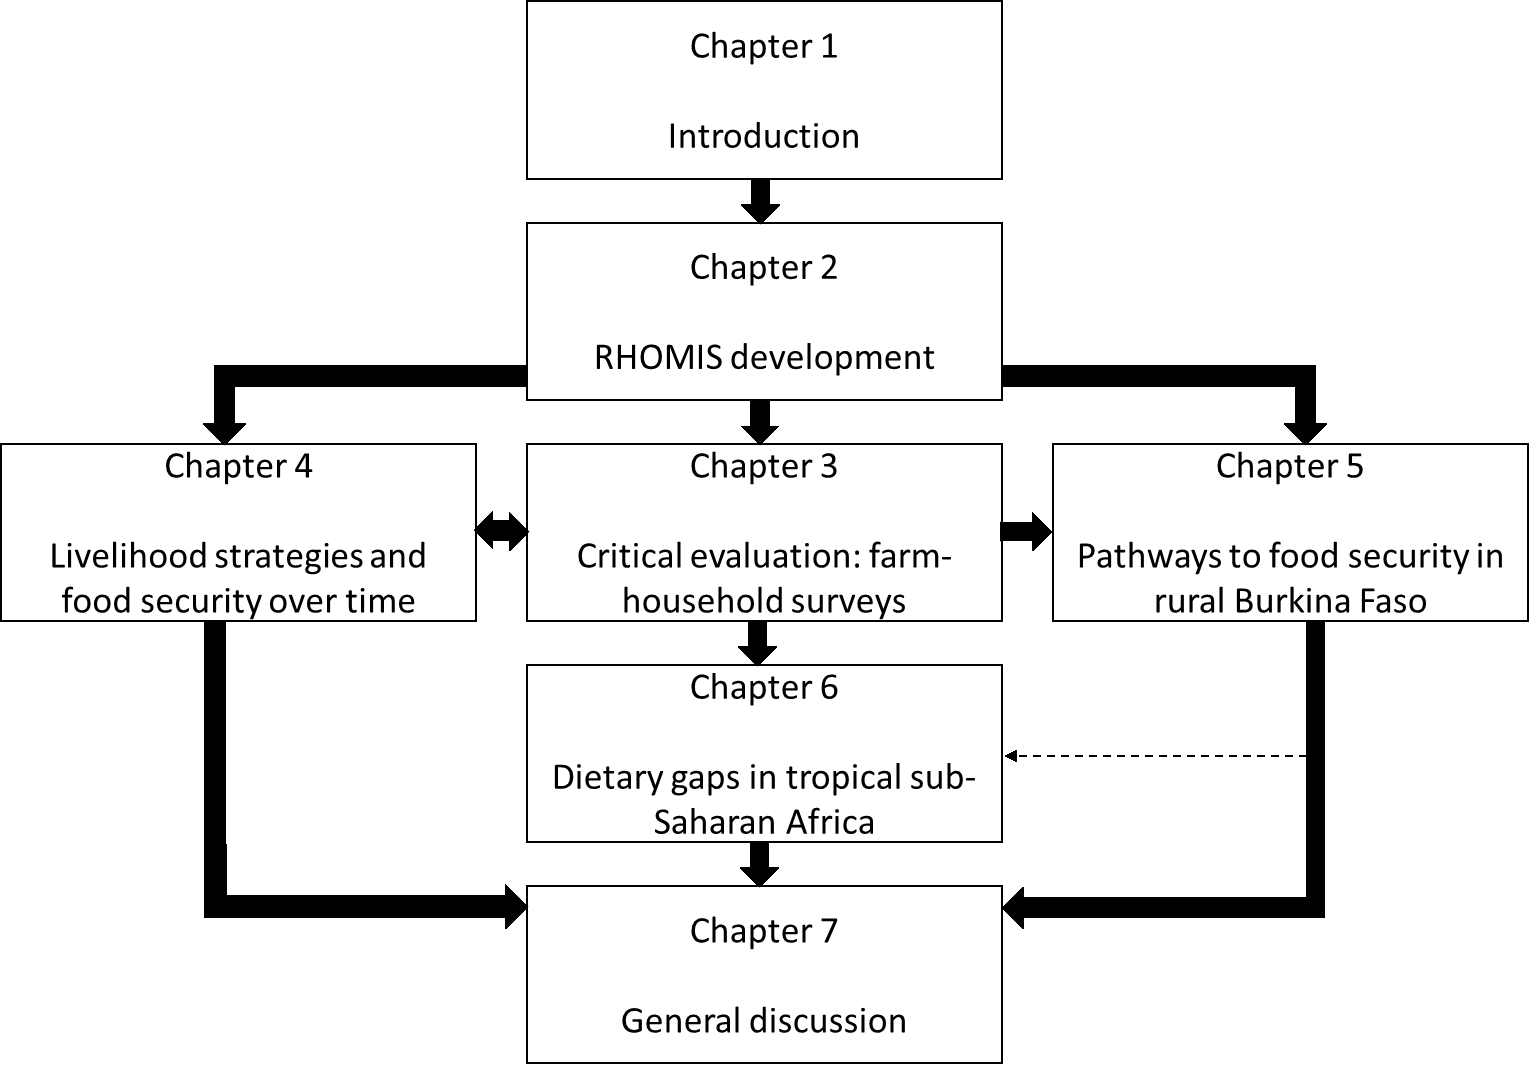
\includegraphics[width=0.8\textwidth]{figs_01/image1.png}

  \captionsetup{singlelinecheck = false, justification=raggedright} %left justify caption
  \label{fig:01_2}
  \caption{Overview of thesis structure}
\end{figure}

\subsubsection{Summary of study sites}

The primary objective of this research is addressed by drawing on harmonised rural household datasets across SSA. Research sites were located exclusively in rural communities and limited to landholding households. Sites were sampled from a diverse range of AEZs, with differing livelihoods and a presence of mixed crop-livestock systems. The study sites are presented in Figure \ref{fig:01_3}. Appendix Table \ref{tab:01_1} summarises the characteristics of study sites. A total of 9,126 households were sampled, of which, 4,323 households were located in warm semi-arid zones, 1,402 households were located in warm sub-humid and humid zones, 250 households were located in a cool semi-arid zone, 1,872 households were located in cool (sub)humid AEZs and two studies spanned multiple AEZs with 1,279 observations. Livestock keeping and staple crop cultivation were prominent livelihood activities in all sites (not represented in Appendix Table \ref{tab:01_1}). The presence of dairy, cash-crops and off-farm income opportunities differed by site. Market orientation and market access also differed. These harmonised rural household datasets were utilised in Chapters 2 to 6, with the majority of observations employed to explore dietary gaps in Chapter 6 (Appendix Table \ref{tab:01_1} summarises which chapter each site relates to).



\begin{figure}
  %\centering
    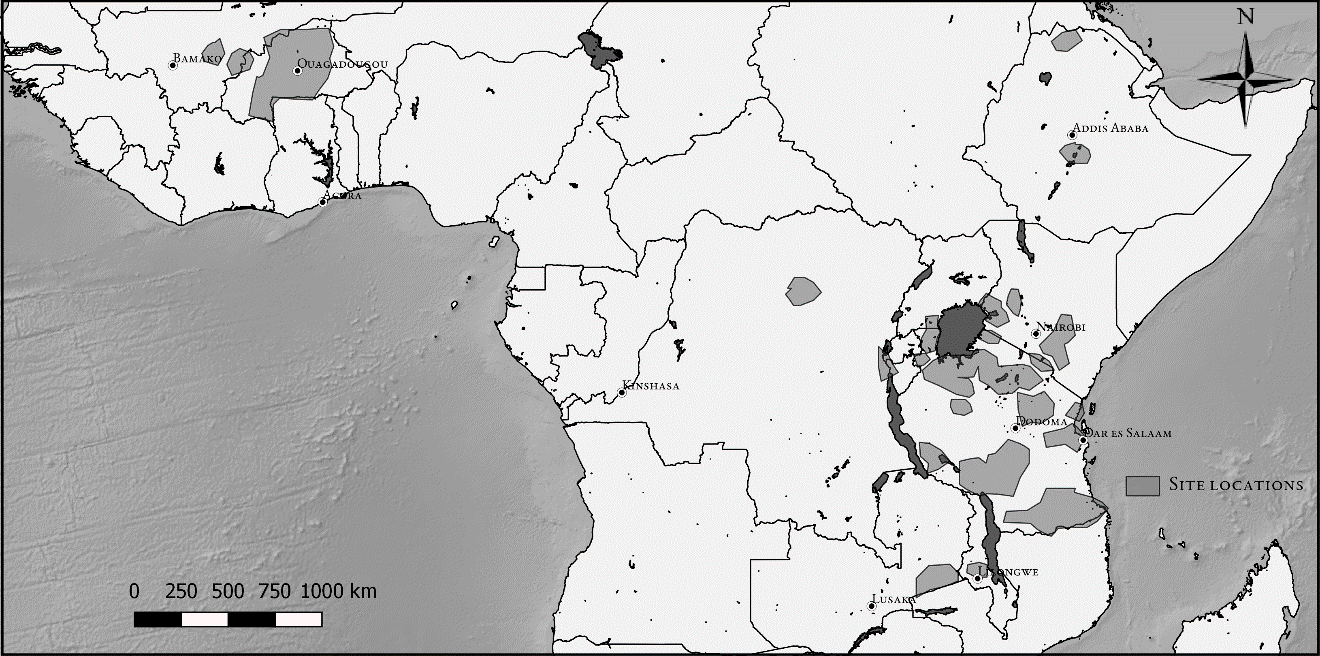
\includegraphics[width=1\textwidth]{figs_01/siteMap.png}
  \captionsetup{singlelinecheck = false, justification=justified} %left justify caption
  \caption{Map of study sites}
    \label{fig:01_3} %Label needs to come after caption
\end{figure}
 % Introduction
\include{02_RHOMIS}
\chapter[Making the most of imperfect farm household data: a critical evaluation of standard information collected in farm household surveys]{Making the most of imperfect farm household data: a critical evaluation of standard information collected in farm household surveys}
\chaptermark{Making the most of imperfect data}
\label{cha:chapter3}
\vspace*{\fill}
This chapter is based on:
\\
\\
% Full citation of the published (or submitted/in review) article
% This refers to the article key in the refs.bib file.
%\bibentry{Fraval2018}
Fraval, S., Hammond, J., Wichern, J., Oosting, S. J., de Boer, I. J. M., Teufel, N., Lannerstad, M., Waha, K., Pagella, T., Rosenstock, T. S., Giller, K. E., Herrero, M., Harris, D., van Wijk, M. T. (2018). Making the most of imperfect data: a critical evaluation of standard information collected in farm household surveys. \textit{Experimental Agriculture}, 1–21. doi:10.1017/S0014479718000388.
\\
\\
Supplementary information is publically available online, accessable via the \href{https://doi.org/10.1017/S0014479718000388}{doi}.


\newpage

\section*{Abstract}
Household surveys are one of the most commonly used tools for generating insight into rural communities. These methods are frequently used in the design and evaluation of agricultural development programmes. Despite their prevalence, few studies have evaluated the quality of such data. We reviewed data from three different farm household surveys deployed in four African countries. We found issues concerning the quality of many reported values and indicators. Surprisingly, even variables which might be considered `easy to estimate' had instances of non-credible observations. Assessment of food security and food self-sufficiency showed that between 29-57\% of observations in the World Bank's 'living standards measurement survey' were deemed beyond credible bounds, while for shorter and more targeted survey tools like the `rural household multiple indicator survey' this value decreased to 25\%. Measurements of maize yields and land owned were found to be less reliable than other stationary variables. This lack of reliability has implications for monitoring food security status, poverty status and the land productivity of households. Despite this rather bleak picture, our analysis shows that if the same farm households are followed over time, the sample sizes needed to detect substantial changes are in the order of hundreds of surveys, and not in the thousands. Our research highlights the value of targeted and systematised household surveys for detecting such changes. Furthermore, ongoing developments in data collection strategies and tools are likely to improve data quality. Aspects that need sustained or improved attention include: survey design (questions and length), transparency of experimental design, effective training, improved coordination between agencies, incorporating mixed modes of data collection and ongoing systematic validation programs. Improvements in the quality of rural statistics will maximise the impact of evidence-based decision making.

\newpage

\section{Introduction}

Smallholder agricultural production in sub-Saharan Africa (SSA) remains a vital source of sustenance, revenue and employment. In the context of forecasted population growth and rapid economic development in many African nations, rural communities will have new opportunities and heightened challenges. Effective, inclusive, and poverty-reducing rural transformation is not an inevitable outcome in future scenarios for SSA nor the broader global rural population (\citealp{IFAD2016}). Rather, pro-poor and equitable rural transformation requires well designed and executed policies and interventions guided by the rural communities themselves.

Household surveys are one of the most commonly used tools for generating insights into rural communities (\citealp{Christiaensen2017}). These tools are used in place of more detailed studies because they are relatively cost-effective. The surveys rely heavily on farmer assessment and recall in place of (more detailed) external monitoring and measurement. The utilisation of low-cost farmer recall enables them to be deployed quickly and at scale which is vital for obtaining representative samples of rural communities and regions. Household surveys can be used for ex-ante and ex-post analyses. Ex-ante applications can be focused on strategic planning purposes, involving prioritisation, characterisation and simulations. Ex-post assessments measure the effect of some 'change'; typical examples include evaluation of new technologies and practices (e.g. those related to cropping, livestock production, land management and natural resource management), or changes to policies and infrastructure (e.g. new roads and market interventions). Ex-post assessments will often assess effects on productivity, decisions (farm management, investments, marketing and off-farm activities) and livelihoods (income, wealth and equity).

Evidence generated to develop and evaluate policies and interventions should be representative of the population of interest, as well as of sufficient quality. Such evidence needs to be founded on a statistically robust sampling protocol that is of sufficient size and designed to minimise sampling error (biases in respondent selection contrary to the population composition) and coverage error (biases from an incomplete sampling frame). The total measurement error of household survey data also consists of random and systematic error, caused by the implementation process of a household survey. Random error can be thought of as instances where repeated measures result in randomly inconsistent values, and systematic errors are errors that are not caused by chance but rather are consistently over or under-reported in a given measurement and observation context. The stages where error can be introduced in a household survey include: designing the data collection tool, training enumerators, soliciting households to participate (which can result in unit non-response error) and collecting information from the farmers -- often based on estimation and remembering past events. As detailed by \citet{Weisburg2005}, there are also specific aspects of survey design, mode of collection, data management and analysis that can introduce random and systematic error.

There is a continuous drive to improve the quality of rural statistics, with a particular focus on reducing random and systematic errors. The central statistical bureaus of many medium and high-income countries have the resources to continuously improve processes and meet domestic data needs and international reporting commitments. For low-income countries, where resources and capacity for agricultural and rural development are constrained, international partners have taken a more active role, for instance by providing guidelines and training (e.g. \citealp{FAO2017}; \citealp{UNFCCC2012}; \citealp{OECD2009}; \citealp{UnitedNationsDepartmentofEconomicandSocialAffairs2005}, as well as the CGIAR and the World Bank). Efforts to improve statistics have addressed the full breadth of issues from experimental design, survey design, enumerator training, data management, analysis and open data policies. The efforts to standardise survey design and indicators are most relevant for this present study because they represent `best-practice' and a process of ongoing improvement. Three comparable survey designs that are multi-topic, multi-purpose and have been internationally applied are: the World Bank's `living standards measurement study' program (LSMS; \citealp{WorldBanka}), the lite version of the `integrated modelling platform for mixed animal crop systems' (IMPACTlite; \citealp{Herrero2007}) and the `rural household multiple indicator survey' (RHOMIS; \citealp{Hammond2017225}). Each of these tools aim to improve the consistency and quality of data collection between sites and within sites.

Despite the importance of rural statistics, there are relatively few studies that systematically evaluate the data quality of household level enumeration. Nevertheless, contributions have been made towards identifying sources and implications of poor data quality. For instance, in a special issue on data quality in Africa, \citet{Jerven2015} concluded that limited resources tend to reduce the quality of statistics and that there are risks of bias at many levels. \citet{Kilic2015} found that survey length has a statistically significant effect on data quality, regardless of topic and question type -- potentially mediated through respondent and enumerator fatigue. \citet{Finn2017} explored methods to detect household survey data fabrication and the implications of fabrication on statistical inference. \citet{Pica-ciamarra2012} reported the perceptions that users (researchers, government departments, ect.) have of the quality of livestock statistics. The effects of gender bias, recall length and respondents' fatigue on response accuracy have also been explored (\citealp{DeNicola2014}; \citealp{Beegle2012}).

Furthermore, the methodological validation program of the LSMS Integrated Survey on Agriculture (LSMS-ISA) program has systematically assessed the deviation of espoused volumes and areas from higher quality measurements (\citealp{Gibson2015}; \citealp{Zezza2014}; \citealp{Kilic2013}; these are akin to the pioneering validation-based improvements made by the USDA-NASS since the 1950s as detailed in \citealp{Fecso2011}). The LSMS-ISA and other `donor-funded surveys' have also provided opportunities to test new methods that can then improve the quality of data collected in national statistical programs (\citealp{Jerven2015}).

The objective of this study was to further our understanding of the quality of rural statistics by critically evaluating a series of reported values and indicators captured in panel and test-retest farm household surveys. We do this by assessing the credibility and reliability of information commonly collected in farm household surveys. The results of this assessment are essential in view of the use of survey data in the scientific literature and more practical, policy formulation and agricultural development planning. Based on our results we suggest ways in which data collection approaches could be improved and the impact of low-quality data can be minimised.

\section{Methods}

We first describe the household survey data we used in the analyses, and then describe in detail the analyses we have performed focusing on credibility, consistency and reliability.

\subsection{Farm household survey data}

Our analysis draws on three comparable multi-topic survey tools: IMPACTlite (\citealp{Rufino2013}), RHOMIS (\citealp{Hammond2017225}) and LSMS-ISA (\citealp{WorldBank}). IMPACTlite was developed in the context of a large-scale climate change mitigation and adaptation research program. The IMPACTlite tool was designed to better understand the implications of mitigation and adaptation strategies ``on livelihoods, food security and the environment'' (\citealp[p.~3]{Rufino2013}).

RHOMIS was developed in response to the general challenges caused by the ``inefficient multiplicity of survey instruments'' (\citealp[p.~30]{Carletto2013}), and in particular inspired by efforts to conduct cross-dataset analyses of farm household surveys in sub-Saharan Africa (\citealp{Frelat2016458}). The tool was designed to capture information efficiently and systematically, allowing the analyst to link farm management to issues of livelihoods, poverty, food security, and gender. The indicators which can be calculated from the survey are generally widely validated and internationally recognised. The scope of the survey was defined in relation to the Sustainable Development Goals, specifically SDGs 1, 2, 5, and 13 (no poverty, zero hunger, gender equality and climate action); but the scope is also of relevance to the assessment of Climate Smart Agriculture principles, and Sustainable Intensification. Data collation and analysis are also components of RHOMIS. There are two overall purposes of the RHOMIS tool: to provide a rapid characterisation of farm systems, for use in ex-ante or ex-post analyses, and secondly, through the building of a large, harmonised dataset from many sites, to permit identification of general principles which can guide the design of rural development interventions. Data from IMPACTlite (2012) and RHOMIS (2015 and 2016) sample the same households and so form test-retest datasets over three sites, namely: Lushoto, Tanzania (n = 149), Wote, Kenya (n = 160) and Nyando, Kenya (n = 161).

The LSMS-ISA tool was developed with a specific focus on Africa with the intention of improving the quality of rural statistics and building the capacity of local statistics offices. The core purpose of a LSMS-ISA implementation is to ``improve the understanding of the links between agriculture, socioeconomic status, and non-farm income activities'' (\citealp[p.~1]{WorldBank}). LSMS-ISA has been implemented in several countries and collected as panel datasets. In this study, the analysis is limited primarily to Uganda (n = 2,374) for the surveys held in 2009/10, 2010/2011 and 2011/12. Analysis of LSMS-ISA data from Tanzania (n = 3,265) and Ethiopia (n= 4,000) from 2010/11 are also included.

The sampling approach differed between the two datasets. IMPACTlite and RHOMIS sampled villages in a 10 x 10 kilometre grid across multiple locations. The household member most aware of farm activities were interviewed in RHOMIS, and in IMPACTlite other household members contributed to specific sections where necessary. The LSMS-ISA for Uganda, in contrast has been designed to be nationally representative (\citealp{UgandaBureauofStatistics2007}; \citealp{UgandaBureauofStatistics}; \citealp{UgandaBureauofStatistics2002}). The household head was interviewed and in his/her absence, a `usual member of the household' capable of responding was interviewed (\citealp{UgandaBureauofStatistics}).

The formulation of questions and mode of data collection also differed in each survey (summarised in Table \ref{tab:03_1}). Perhaps most notably, LSMS-ISA revisits households on a seasonal basis within a 12-month period, whereas IMPACTlite and RHOMIS were conducted only once with multiple recall periods. Surveys incorporated questions on household demographics, farm characteristics, product marketing, income and household diet diversity (in the case of IMPACTlite and RHOMIS, this was calculated based on \citealp{Swindale2006}). All variables assessed in this study were answered by all respondents. In addition, zero values (for land holdings, maize yield and livestock) were crosschecked with other sections of the surveys to identify potential item non-responses -- all zero values were corroborated.



\begin{table}
  \captionsetup{singlelinecheck = false, justification=justified} %left justify caption
  \caption{%
  Characteristics, question formulation and relevant period of survey tools
  }
  \small
  \centering
  \label{tab:03_1}
\begin{tabular}{L{1.8cm} L{2cm} L{3.33cm} L{3.33cm} L{3.33cm}}
  %{
%p{\dimexpr 0.12\linewidth-2\tabcolsep}
%p{\dimexpr 0.18\linewidth-2\tabcolsep}
%p{\dimexpr 0.24\linewidth-2\tabcolsep}
%p{\dimexpr 0.23\linewidth-2\tabcolsep}
%p{\dimexpr 0.23\linewidth-2\tabcolsep}}
\toprule
 & & IMPACTlite & RHOMIS & LSMS-ISA \\
 \midrule
\multicolumn{2}{l}{Locations} & Kenya, Tanzania & Kenya, Tanzania & Uganda \\
\multicolumn{2}{l}{Survey rounds} & 1 & 1 & 3 revisits \\
\multicolumn{2}{l}{Observations} & 470 & 470 & 2,374 \\
\multicolumn{2}{l}{Representativeness} & \mbox{Development domains} & \mbox{Development domains} & Nationally \\
\multicolumn{2}{l}{Duration} & 2.5 - 3 hours & 45 min to 1 hour & Unknown \\
\arrayrulecolor{black!30}\midrule
Crop harvest & Question formulation & Subplot harvest by crop and & Crop harvest -- local volume units & Subplot harvest by crop \\
 & Relevant period & Seasonal & Seasonal and annual & Seasonal - revisits \\
 \arrayrulecolor{black!30}\midrule
Crop area planted & Question formulation & Area planted by crop & Area planted by crop -- local area units & Area planted by crop \\
 & Relevant period & Seasonal & Seasonal and annual & Seasonal - revisits \\
 \arrayrulecolor{black!30}\midrule
Price & Question formulation & Price per kg & Price per kg/tonne/unit or total value & Value of yield in plot \\
 & Relevant period & Seasonal & Annual & Seasonal - revisits \\
 \arrayrulecolor{black!30}\midrule
Household head age & Question formulation & Date of birth all members & Age of head & Date of birth all members \\
 & Relevant period & As of interview date & As of interview date & As of interview date \\
 \arrayrulecolor{black!30}\midrule
Household size & Question formulation & Full household roster & By age category & Full household roster \\
 & Relevant period & {\textgreater} 1 season & {\textgreater} 3 months per year & 12 months \\
 \arrayrulecolor{black!30}\midrule
Livestock holdings & Question formulation & Full list converted to TLU & Full list converted to TLU & Full list converted to TLU \\
 & Relevant period & Current holdings & Current holdings & Current holdings \\
 \arrayrulecolor{black!30}\midrule
Land owned & Question formulation & Parcel size & Total land owned & Parcel size \\
 & Relevant period & Annual & Annual & Annual \\
 \arrayrulecolor{black!30}\midrule
Off-farm income & Question formulation & Full income register & Proportion of total & Full income register \\
 & Relevant period & Annual/Monthly/week & Annual & Annual \\
 \arrayrulecolor{black!30}\midrule
Household diet diversity & Question formulation & Itemised food list open question & 12 or 10 category list prompted & 61 item food list \\
 & Relevant period & Seasonal & Seasonal & 7 day recall \\
\arrayrulecolor{black}\bottomrule
\end{tabular}
\end{table}

\subsection{Data analyses}

We use the household data described to assess their credibility (in terms of inaccuracies) and reliability (measurement precision; \citealp{Alwin2006}; \citealp{Evans1995}). We first assess the credibility of observations in one survey round, which also gives us insight into systematic errors. Credibility (identifying inaccurate observations) in this context is concerned with whether values fall outside acceptable bounds. We then assess the consistency of measurements between two rounds with two household survey instruments that are similar in complexity and are focused on single site applications, i.e. RHOMIS and IMPACTlite. For a more robust assessment of consistency, we also model the reliability of the LSMS-ISA dataset using three rounds of survey data. This measure of reliability better accounts for survey round specific systematic errors, but does not distinguish between true population scale temporal volatility, random error and non-survey round based systematic error.

To conclude our analysis, we assess the implications of varying levels of reliability on required sample sizes. Although all of these analyses give insight into the possible existence of systematic errors, none of the methods above will allow us to really quantify these. For that mixed method approaches are needed, e.g. weighed crop yields or GPS based field size estimates, where one can quantify the deviation between farmer recall based information and `reality'. This lies outside the scope of this study.

\subsection{Credibility analysis}

Crop yields and market prices were used to assess the credibility of farmer reported and estimated values. As indicated in Table \ref{tab:03_1}, we calculated crop yields as a composite of farmer reported harvest volumes and area planted, and market prices could be enumerated as the unit price or a composite of total value and volume sold. Due to the limited availability of secondary data, crop productivity and market prices were only assessed for maize (\textit{Zea mays} L.), quantifying the yield (kg ha$^{-1}$) and the farm-gate price per kilogram for each farm household. Yields calculated from farmer reported harvest volumes and area planted were compared with historical yield estimates (from fertilised crop trials and government monitored plots) from the Global Yield Gap Atlas (GYGA, n.d.). Historical yield estimates compiled in the GYGA formed the basis for setting lower credible bounds. The threshold was set at 10\% of the average historical GYGA yield for the same climate-zone and country. Simulated water-limited yield potential formed the basis for setting credible upper bounds. It is unlikely that enumerated yields exceed the simulated potential. Historical, potential and survey reported yields were compared on a country and climate-zone basis (using the GYGA climate zones). The historical yields in Uganda, for example, ranged from 0.7 tonnes per ha to 1.31 tonnes per ha (a summary of used thresholds is provided in SI Table 1).

Farm-gate prices were compared with the average price for each location (i.e. Lushoto, Wote, Nyando, Kampala, western Uganda, ect.) and survey tool as well as the wholesale market prices in major cities (Kampala in Uganda and Nairobi in Kenya and Tanzania; sourced from \citealp{FoodandAgricuturalOrganization2017}). In this component of our credibility analysis, we assume a high degree of market integration, where there is a close association with farm gate price, regional price and market price. Prices in the surveys were also averaged across seasons to give an annual average. Lower limits were set at 10\% of the average survey prices for a given location; upper limits were set at the maximum wholesale market price. A summary of price thresholds is provided in Supplementary Information Table 2. The statistics on wholesale market prices also have errors associated with them, this analysis only provides information about the uncertainty surrounding farmer estimates rather than an absolute benchmarking of data quality.

To assess the consequences of data credibility for more complex, constructed indicators, we examine the commonly used indicators of food self-sufficiency and potential food availability (as detailed in \citealp{Frelat2016458}). The food availability indicator (FA) is a quantification of the potential kilocalories available for each male adult equivalent per day consumed from farm production, and from cash obtained through the sale of farm produce and off-farm income, where all income is converted to a calorific value based on the cost of a local staple crop. For our calculations of FA, we used the median farm gate price for each location and time period. Results of these calculations can be used to perform a combined data quality assessment of information obtained on crop and livestock production, sales, consumption and off-farm income. Two problems with this composite indicator are commonly encountered. First, an underestimation of the calorie availability at the lower end of the scale, suggesting an extreme level of starvation. Although this may be a true representation of some households, it can also be an indication of missing information on income or food consumption. Second, there can be a substantial over-estimation of consumption of crop and livestock products for a large number of households (i.e. food self-sufficiency), indicating problems with yield, consumption or household size data. The lower bound threshold for credible food availability was set at 1250 kilocalories (kcal) per male adult equivalent per day, which is below the basal metabolic rate for adult males (approximately 1590 kcal for a 60 kg male; \citealp{FoodandAgricuturalOrganization2001}). Two upper bounds for credible food self-sufficiency were set: a) 3500 kcal per adult equivalent per day, representing the average intake of developed nations (\citealp{OrganisationforEconomicCo-operationandDevelopmentOECD2017}), and; b) 5000 kcal, which is double the approximate requirement for an adult male.

The results from \citet{Rosenstock2017} provide an example of extremes in food availability and food self-sufficiency for households in northern Ghana. This case is represented here in Figure \ref{fig:03_1} as the ratio of food availability, where the value 1 represents a case where 2,500 kilocalories are provided for each male adult equivalent (indicated with a horizontal dotted line). Also represented is the ratio of food availability sourced directly from farm production (the grey bars). Instances of apparent starvation are increasingly severe as the ratio decreases below 1, which eventually declines below the basal metabolic rate for adult males. Over-estimated consumption is apparent in households that have more energy sourced directly from the farm than is required (grey bars larger than 1).

\begin{figure}
  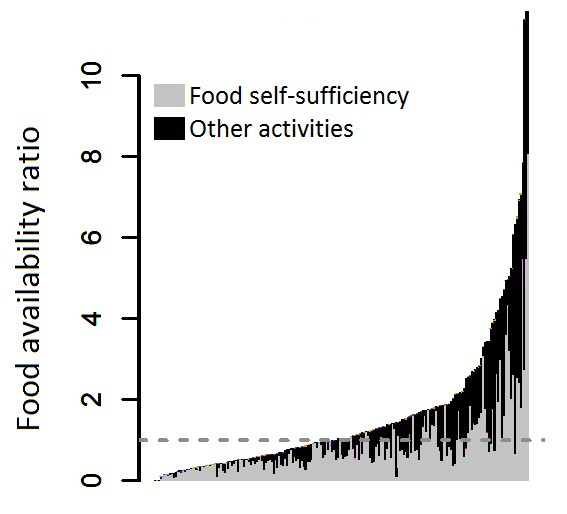
\includegraphics[width=0.5\textwidth]{figs_03/image1.png}
  \captionsetup{singlelinecheck = off, justification=justified} %left justify caption
  \caption{Food availability, food self-sufficiency and household energy needs: an example of unreliable values}
  \small
  %\raggedright
  \vspace*{-3mm}
  \caption*{Dashed line represents a case where 2,500 kilocalories are provided for each male adult equivalent \\
    (Source: \citealp{Rosenstock2017}; based on 200 households in northern Ghana)}
  \label{fig:03_1}
\end{figure}


\subsection{Consistency and reliability analyses}

In the consistency and reliability analyses we included variables that we would expect to be: a) highly consistent (age of the household head), b) relatively stationary in East Africa over the whole population over short time periods, including household size, productive assets (land owned and livestock holdings) and crop yields, and c) those that may be more variable (off-farm income, food availability and food self-sufficiency). Age of household head is expected to be highly consistent after accounting for the time elapsed between survey rounds and whether there was a change in household head. Household size was expected to be relatively stationary in East Africa given that death rates have been estimated to be less than 1\% per annum (\citealp{CIA2016a}) and the rate of urbanisation estimated to be less than 5.5\% per annum (\citealp{CIA2016}). Productive assets are also expected to be relatively stationary due to their livelihood and cultural value -- for both land (\citealp{Jayne2016}) and livestock (\citealp{Thornton2015}). Livestock holdings, however, are expected to be more temporally variable than land holdings due to their role in financing large expenditures, cultural utility (i.e. bride-wealth) and exposure to climatic and disease risks (ibid.). Similarly, crop yields are expected to be temporally stable (at a population level) in the absence of extreme weather events (\citealp{Gollin2006}). During the periods of observation, there were instances of extreme weather events, with a severe drought impacting northern Kenya and north-eastern Uganda (potentially impacting {\textless} 0.5\% of households in LSMS-ISA Uganda) and some evidence of increased extreme precipitation events in western Kenya, but to our knowledge this did not affect the sampled households (\citealp{Gebrechorkos2018}). Climatic conditions were consistent over the two survey rounds in Tanzania (\citealp{Fraval2018a}).

We explored the consistency of data collected in farm household surveys between two points in time, comparing respectively, IMPACTlite (2012) with RHOMIS (2015/16), and LSMS-ISA (2009/10 and 2011/12). Summary statistics of these changes between initial survey and revisit are provided in supplementary Information Table 3. In the absence of survey round specific biases, the correlations in these consistency results would provide a measure of reliability (\citealp{Alwin2006}). As this is not the case, we can only interpret the strength of correlation as a measure of consistency, rather than reliability. Spearman's correlation was used to assess association, as it is less sensitive to extreme non-credible values.

Reliability was more formally modelled using the core variables and derived indicators quantified from LSMS-ISA Uganda (2009/10, 2010/11, 2011/12), excluding some non-credible values. We used an approach described by \citet{Shrout1979} that calculates intraclass correlation (ICC). In this specification, we assume the following linear model:

\begin{equation}
\tag{3.1}
x_{ij}=\mu +b_{j}+w_{ij}
\end{equation}

Where x$_{\mathrm{ij}}$ is the value in the ith survey round (i = 1, 2, 3) of j household (j = 1, {\ldots}, n); $\mu$ is the population mean; b$_{\mathrm{j}}$ is the difference from $\mu$ to the jth household's mean across the survey rounds; w$_{\mathrm{ij}}$ is the residual, equal to the sum of the effects of survey round, survey round-household interaction, and error. The intraclass correlation is then estimated as follows:

\begin{equation}
\tag{3.2}
ICC=\frac{MSB-MSW}{MSB}
\end{equation}

Where MSB is the mean square between (sum of square total/obs) and MSW is mean square within, calculated as:

\begin{equation}
\tag{3.3}
\mathrm{MSW}=\frac{SS_{round}+SS_{resid}}{df_{round}+df_{resid}}
\end{equation}

For this analysis, some non-credible observations were excluded as they had a disproportionate influence on the linear models. Observations with off-farm income above US\$60,000 in one survey round were excluded (n = 1), as were maize yields above 15 tonnes per ha (n = 33), livestock holdings (TLU {\textgreater} 100, n = 3), land owned (ha {\textgreater} 100; n = 2) and food availability (FA {\textgreater} 1,500,000 kcal, n = 2). The reliability analysis was implemented using the psych package in R (\citealp{Revelle2017}). This analysis resulted in a reliability estimate ranging between 0 (`low reliability') and 1 (`high reliability') together with a 95\% confidence interval of this estimate. The three methodological steps and associated datasets, locations and years are summarised in Table \ref{tab:03_2}.



\begin{table}[H]
  \captionsetup{singlelinecheck = false, justification=justified} %left justify caption
  \caption{
  Summary of analysis, datasets and variables
  }
  \small
  \label{tab:03_2}
\begin{tabularx}{\textwidth}{@{}lllYYY@{}}
%  {
%p{\dimexpr 0.2\linewidth-2\tabcolsep}
%p{\dimexpr 0.21\linewidth-2\tabcolsep}
%p{\dimexpr 0.1\linewidth-2\tabcolsep}
%p{\dimexpr 0.16\linewidth-2\tabcolsep}
%p{\dimexpr 0.16\linewidth-2\tabcolsep}
%p{\dimexpr 0.16\linewidth-2\tabcolsep}}
\toprule
Survey tool & Country & Year & \multirow{2}{2cm}{Credibility (one round)} & Consistency (two rounds) & \multirow{2}{2.5cm}{Reliability (three rounds)} \\
\midrule
IMPACTlite & Kenya \& Tanzania & 2012 & x & a & \\
RHOMIS & Kenya \& Tanzania & 2015/16 & x & a & \\
LSMS-ISA & Uganda & 2009/10 & & b & c \\
LSMS-ISA & Uganda & 2010/11 & x & & c \\
LSMS-ISA & Uganda & 2011/12 & & b & c \\
LSMS-ISA & Tanzania & 2010/11 & x & & \\
LSMS-ISA & Ethiopia & 2010/11 & x & & \\
\bottomrule
\end{tabularx}
  \footnotesize
     \raggedright x = used in credibility assessment\\
     a, b, c = dataset, where two or three survey rounds are used in an analysis
\end{table}

%$\mathrm{ES}=\text{populationES}\times \sqrt \mathrm{r}$

The relationship between sample reliability, effect size and sample size was simulated using the `pwr' package in R (\citealp{Champely2018}), where reliability is mediated through the effect size ($ES = populationES \times \sqrt{r}$, assuming equal variace and sample sizes; \citealp{Phillips2016}). Using the pwr package, we simulated both a paired (panel type of data) and two-sample (Randomised Control Trial type of data) t-tests to quantify detectable differences for the core variables and derived indicators of which we have quantified reliability and uncertainty estimates. The simulated t-tests assumed a Type II error rate of 20\% (Power of 0.8) and a Type I error rate of 5\% (${\upalpha}$ of 0.05).

\section{Results}

\subsection{Credible bounds of core variables and derived indicators}

Yields and prices were highly variable in each of the three farm household survey tools. This variability across a wide range of crops could reflect agro-climatic or management differences, market volatility, as well as biases and errors introduced by the survey tool, enumerator or the respondent (\citealp{UnitedNationsDepartmentofEconomicandSocialAffairs2005}; \citealp{Mathiowetz2001}). This section provides a summary of non-credible values for yields (Table \ref{tab:03_3}), prices (Table \ref{tab:03_4}), food availability and food self-sufficiency (Table \ref{tab:03_5}).

Comparing our calculated maize yields with historical yield statistics compiled in the Global Yield Gap Atlas gives a reference point to assess yield estimates for each of the three survey tools. IMPACTlite had the highest proportion of households with crop yields less than 10\% of GYGA historical maize yields, followed by RHOMIS and then LSMS-ISA (Table \ref{tab:03_3}). On the other extreme, LSMS-ISA had the most substantial proportion of yields exceeding the simulated water-limited potential yield for the region -- occurring in 7\% of households. Four percent of households in LSMS-ISA 2010/11 Uganda exceeded potential maize yields and an additional 3\% were double this potential yield (Table \ref{tab:03_3}).



\begin{table}
  \captionsetup{singlelinecheck = false, justification=justified} %left justify caption
  \caption{Credibility of maize yield data: comparing enumerated yields with historical yields and water-limited potential yields, by survey tool* (proportion of households)
  }
  \small
  \label{tab:03_3}
\begin{tabularx}{\textwidth}{@{}lYYYY@{}}
%  {
%p{\dimexpr 0.22\linewidth-2\tabcolsep}
%p{\dimexpr 0.19\linewidth-2\tabcolsep}
%p{\dimexpr 0.27\linewidth-2\tabcolsep}
%p{\dimexpr 0.19\linewidth-2\tabcolsep}
%p{\dimexpr 0.13\linewidth-2\tabcolsep}}
\toprule
~ & Less than 10\% of historical yields & Greater than potential yield \& less than double & Double potential yield & Within bounds \\
\midrule
IMPACTlite 2012 & 0.43 & 0.00 & 0.01 & 0.56 \\
RHOMIS 2015/16 & 0.12 & 0.00 & 0.00 & 0.88 \\
LSMS-ISA 2010/11 & 0.03 & 0.04 & 0.03 & 0.90 \\
\bottomrule
\end{tabularx}
\footnotesize
\raggedright *Impact lite and RHOMIS include sites from Kenya and Tanzania, LSMS-ISA is limited to Uganda
\end{table}



Exceeding the simulated potential yield is possible, but unlikely -- even historical yields in optimal growing conditions were never more than 50\% of simulated potential yields (results not shown). It is more difficult, however, to assess the credibility of calculated yields at the lower end of the scale, which are far more prevalent. Comparing maize yields from the same sites from both IMPACTlite (2012) and RHOMIS (2015/16) data, 62\% of households that had yields less than one tonne per hectare had those low yields in both surveys. An additional tonne per hectare was reported by 27\% of households in the RHOMIS (2015/16) survey.

The farm-gate price per kilogram of maize was compared with the median price for each data collection instance as well as the market wholesale price (sourced from \citealp{FoodandAgricuturalOrganization2017}). The average market wholesale price of maize in Kampala, Uganda during the year of data collection was 20 US cents per kilogram, with a minimum of 11 cents. Approximately 15\% of LSMS-ISA (2011/12) Uganda crop prices exceeded the maximum wholesale price, and 1\% was below the lower threshold. There were also such potential credibility issues in the IMPACTlite and RHOMIS datasets, with maize prices exceeding maximum wholesale prices in 53\% and 14\% of cases respectively (Table \ref{tab:03_4}). Similar to yield, the lower range on price is more difficult to assess. There are product quality aspects, market timing and geographical differences also influencing price (particularly for LSMS-ISA in Uganda which aims to be nationally representative). These aspects could result in farm gate prices well below the regional average.



\begin{table}
  \captionsetup{singlelinecheck = false, justification=justified} %left justify caption
  \caption{
   Credibility of maize price data: comparing enumerated prices with average survey prices and wholesale market prices by survey tool* (proportion of households)
  }
  \small
  \label{tab:03_4}
\begin{tabularx}{\textwidth}{@{}lYYYY@{}}
  %{\textwidth}{
%p{\dimexpr 0.22\linewidth-2\tabcolsep}
%p{\dimexpr 0.19\linewidth-2\tabcolsep}
%p{\dimexpr 0.27\linewidth-2\tabcolsep}
%p{\dimexpr 0.19\linewidth-2\tabcolsep}
%p{\dimexpr 0.13\linewidth-2\tabcolsep}}
\toprule
~ & less than 10\% of average prices of survey & Greater than maximum wholesale price \& less than double & Double maximum wholesale price & Within bounds \\
\midrule
IMPACTlite 2012 & 0.03 & 0.50 & 0.03 & 0.43 \\
RHOMIS 2015/16 & 0.02 & 0.09 & 0.05 & 0.84 \\
LSMS-ISA 2010/11 & 0.01 & 0.11 & 0.04 & 0.84 \\
\bottomrule
\end{tabularx}
\footnotesize
\raggedright{*Impact lite and RHOMIS include sites from Kenya and Tanzania, LSMS-ISA is limited to Uganda}
\end{table}



Non-credible values in core variables will propagate through to composite indicators, such as food self-sufficiency and potential Food Availability (FA). Specifically, non-credible values in farm production, area planted, product marketing, off-farm income and household size can be compounded in these indicators. Table \ref{tab:03_5} shows the proportion of households that have non-credible food availability and self-sufficiency values (defined by being below half or more than double the energy demands of the household). Instances of non-credible FA values exist in all survey implementations, but more so in IMPACTlite. LSMS-ISA Uganda and LSMS-ISA Tanzania had the most non-credible food self-sufficiency values. LSMS-ISA Tanzania and Ethiopia are included in this table as an example of the variability in data quality generated with the same survey tool. LSMS-ISA Tanzania and Ethiopia appear to provide much lower quality food availability and food self-sufficiency estimates as compared to LSMS-ISA Uganda.





\begin{table}
  \captionsetup{singlelinecheck = false, justification=justified} %left justify caption
  \caption{
  Credibility of food availability (FA) and food self-sufficiency (FSS) by survey tool (proportion of households)
  }
  \small
  \label{tab:03_5}
\begin{tabularx}{\textwidth}{@{}lYYYY@{}} %{
%p{\dimexpr 0.29\linewidth-2\tabcolsep}
%p{\dimexpr 0.21\linewidth-2\tabcolsep}
%p{\dimexpr 0.27\linewidth-2\tabcolsep}
%p{\dimexpr 0.13\linewidth-2\tabcolsep}
%p{\dimexpr 0.09\linewidth-2\tabcolsep}}
\toprule
~ & Food availability less than 1250 kcal adult equivalent$^{-1}$ & FSS above OECD average \& Less than double & FSS double 2500 kcal adult equivalent$^{-1}$ & Within bounds \\
\midrule
IMPACTlite 2012 & 0.39 & 0.05 & 0.04 & 0.52 \\
RHOMIS 2015/16 & 0.15 & 0.06 & 0.04 & 0.75 \\
LSMS-ISA Uganda 2010/11 & 0.12 & 0.07 & 0.14 & 0.66 \\
LSMS-ISA Tanzania 2010/11 & 0.20 & 0.06 & 0.07 & 0.67 \\
LSMS-ISA Ethiopia 2010/11 & 0.40 & 0.02 & 0.07 & 0.51 \\
\bottomrule
\end{tabularx}
\footnotesize
\raggedright *Impact lite and RHOMIS include sites from Kenya and Tanzania
\end{table}


\newpage

\subsection{Consistency of core variable measurements and derived indicators over time}

After accounting for the time elapsed between the two surveys and excluding households where the household head had changed (LSMS-ISA, n = 168) or household head gender was different between rounds (IMPACTlite 2012-RHOMIS 2015/16, n = 67), 84\% of households in LSMS-ISA Uganda were within one year of the expected age. In contrast, only 47\% were within the expected range of one year in IMPACTlite-RHOMIS. The relationship between the successive surveys, as shown by Spearman's correlation coefficient in Figure \ref{fig:03_2}a, is strong in both LSMS-ISA (r = 0.99) and IMPACTlite-RHOMIS (r = 0.93). However, there were instances of substantial differences, with 1\% of households in LSMS-ISA, and 8\% of households in IMPACTlite-RHOMIS being 10 years greater or less at revisit than the expected age.

Household size was highly correlated between the 2009/10 and 2011/12 surveys in Uganda (r = 0.9) and moderately correlated in IMPACTlite-RHOMIS (r = 0.51; Figure \ref{fig:03_2}b). The majority of households in each dataset, however, remained within one adult equivalent of the initial visit. For instance, 62\% of households remained within one adult equivalent in LSMS-ISA and 55\% in IMPACTlite-RHOMIS (results not shown). There were isolated cases of extreme increases in each dataset, with the maximum increase in LSMS-ISA being 11 adult equivalents and 14 in IMPACTlite-RHOMIS (Figure \ref{fig:03_2}b).

\begin{figure}
  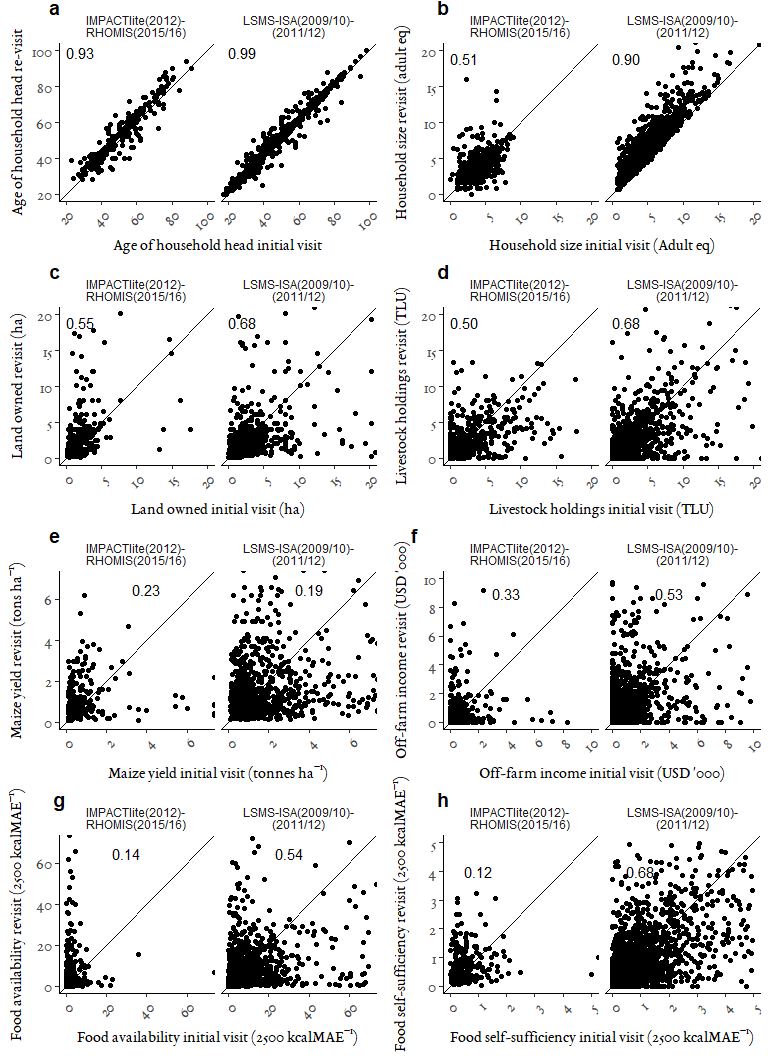
\includegraphics[width=1\textwidth]{figs_03/image2.png}
  \captionsetup{singlelinecheck = off, justification=justified} %left justify caption
  \caption{Consistency between IMPACTlite (2012)-RHOMIS (2015/16) in Kenya and Tanzania and LSMS-ISA (2009/10-2011/12) in Uganda*}
  \label{fig:03_2}
  %\small
  %\raggedright
  \vspace*{-3mm}
  \caption*{*Spearman's correlation coefficient (initial visit to revisit) indicated on each respective plot}
\end{figure}


Land owned in LSMS-ISA survey rounds had a higher correlation (r = 0.68) than IMPACTlite-RHOMIS (r = 0.55; Figure \ref{fig:03_2}c). Isolated cases of extreme changes in land owned were present in LSMS-ISA. Livestock holdings in LSMS-ISA Uganda had a Spearman's correlation coefficient of 0.68 between survey rounds. The level of association between rounds was lower in IMPACTlite-RHOMIS (r = 0.50; Figure \ref{fig:03_2}d). There was a similar level of correlation for maize yields in IMPACTlite-RHOMIS (r = 0.23) and LSMS-ISA (r = 0.19; Figure \ref{fig:03_2}e).

Off-farm income was moderately correlated between rounds in LSMS-ISA (r = 0.53) and less so in IMPACTlite-RHOMIS (r = 0.33; Figure \ref{fig:03_2}f). Changes in off-farm income of US\$5,000 or more occurred in 6\% of the households in Uganda and 2\% in IMPACTlite-RHOMIS. Households in LSMS-ISA, span a wide geographical range with varying proximity to urban locations which may explain such outliers.

Food availability at initial visit and revisit had a moderate association in LSMS-ISA (r = 0.54) and less so in IMPACTlite-RHOMIS (r = 0.14; Figure \ref{fig:03_2}g). There were instances of outliers in both survey comparisons; these few cases, however, could be realistic given large changes in on-farm and off-farm income. Food self-sufficiency followed a similar pattern to food availability, with LSMS-ISA having a having a greater level of correlation between survey rounds (r = 0.68) when compared to IMPACTlite-RHOMIS (r = 0.12; Figure \ref{fig:03_2}h).

Household diet diversity in the IMPACTlite-RHOMIS surveys also provides a notable case of inconsistency between survey rounds. For example, median increases in diet diversity range from three food categories in the lean peiod, and up to six food categories in the Tanzanian post-harvest period. As desirable as leaps in diet diversity are, it is unlikely to observe such a change over a short space of time in these communities (\citealp{IFAD2016}). Figure \ref{fig:03_3} shows the differences between the survey rounds in both periods for Tanzania as an example, where the same applies for IMPACTlite-RHOMIS in Kenya. The initial visit has instances where common food categories (e.g. fats and oils) are supposedly not consumed at all. The likely causes of these differences relate to survey design and duration. IMPACTlite enumerated a wide range of food items (not food groups) asked as an open question. Furthermore, these questions came at the end of a three-hour interview, potentially resulting in respondent fatigue. RHOMIS, on the other hand, asked about these food groups specifically and was completed within an hour.

\begin{figure}[H]
  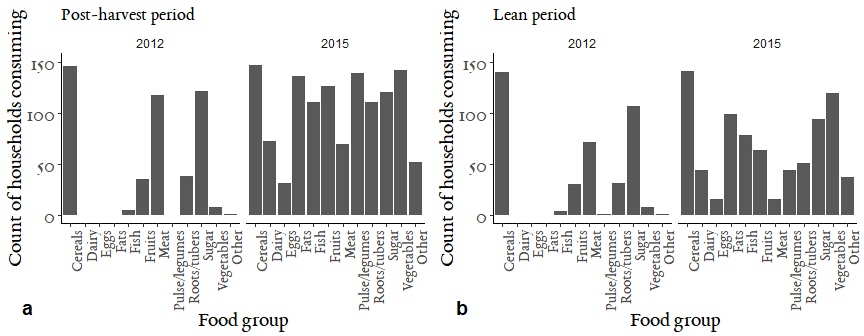
\includegraphics[width=1\textwidth]{figs_03/image3_v2.png}
  \captionsetup{singlelinecheck = off, justification=justified}
  \caption{Diet diversity by category and period in IMPACTlite-RHOMIS Tanzania}
  \label{fig:03_3}
\end{figure}


\subsection{Reliability of variables in LSMS-ISA Uganda}

Modelling the reliability of variables explored in the consistency analysis provides further insight into the three waves in the LSMS-ISA Uganda case. The model outputs suggest a high degree of reliability for age, household size and livestock holdings (Figure \ref{fig:03_4}); land owned was less reliable than these other stationary variables and maize yield was one of the least reliable variables. It is more difficult to evaluate the reliability estimates of off-farm income, food availability and food self-sufficiency. The paucity of information about the temporal stability of these variables (despite efforts to assess the quality of variables such as income -- notably by \citealp{Neri2012}; \citealp{Fisher2010}; \citealp{Juster2007}; \citealp{Moore2000}) make it difficult to identify whether the reliability scores of these three variables are influenced by true population level temporal volatility, but it is clear that the reliability of these variables is low.

\begin{figure}[H]
  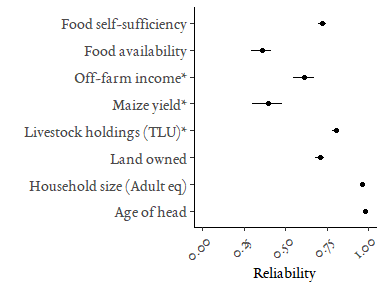
\includegraphics[width=0.5\textwidth]{figs_03/image4.png}
  \captionsetup{singlelinecheck = off, justification=justified}
    \caption{Reliability of initial visit variables in the living standards measurement survey, Uganda: output from intraclass correlations with 95\% Confidence Intervals}
  \label{fig:03_4}
  \small
  %\raggedright
  \vspace*{-6mm}
  \caption*{* Limited to households that were {\textgreater} 0 in each survey round. 27\% of households had off-farm income in all 3 rounds, 75\% cultivated maize, 60\% kept livestock}
\end{figure}
\vspace*{-6mm}



The reliability of these variables will ultimately affect inference as it reduces the power of tests (increasing Type II error) and inflates error estimates in multivariate analyses. Additionally, in instances of new studies using existing data for setting required sample sizes, consideration needs to be given to the reliability of available variables and how the proposed study will differ in terms of measurement error; a new study with a coarser measurement tool will require a larger sample than a previous study with more accurate measures. Figure \ref{fig:03_5} shows the relationship between sample reliability, effect size and sample size for paired and two-sample t-tests. For example, the sample size required to detect a relatively small effect size (0.2) in a paired test with a Type II error rate of 20\% and Type I error rate of 5\%, will be 220 with a reliability of 0.9 (as we see for household size) and 983 households for a reliability of 0.2 (as we see for off-farm income and crop yield). These sample sizes will be higher when design effects are incorporated and when two-sample tests are needed.

\begin{figure}[H]
  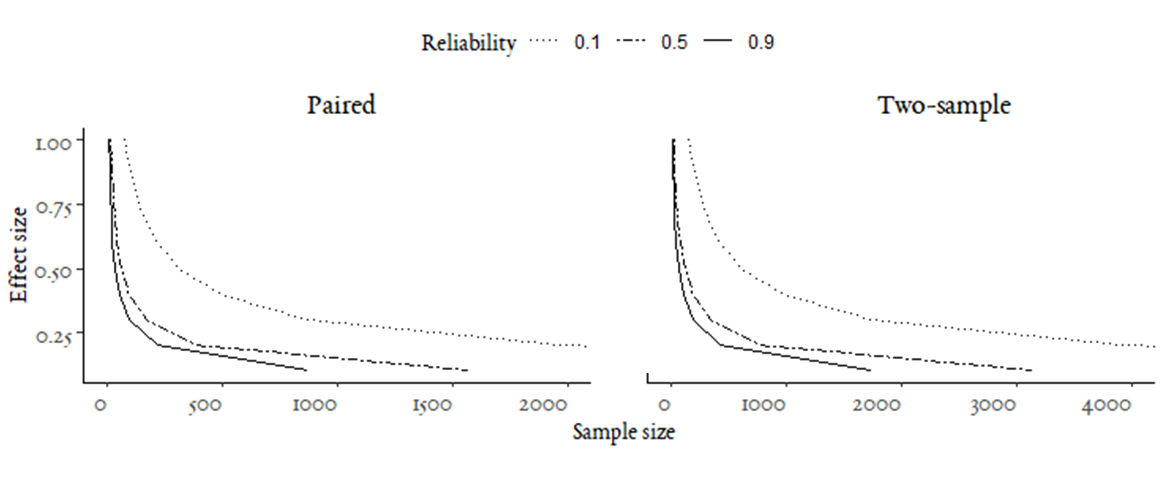
\includegraphics[width=0.8\textwidth]{figs_03/image5.png}
  \captionsetup{singlelinecheck = off, justification=justified}
  \caption{Sample size and effect size given different levels of reliability for t-test (power = 0.8; ${\upalpha}$ = 0.05)}
  \label{fig:03_5}
\end{figure}


\section{Discussion}

\subsection{Credibility of crop yield and market price}

Using data from three cross-sectional farm household survey approaches, we assessed the credibility and reliability of core variables and derived indicators. This study has identified quality limitations in each survey tool -- with LSMS-ISA and RHOMIS staying within credible bounds more frequently than IMPACTlite (Tables \ref{tab:03_3} and \ref{tab:03_4}). The higher performance of these two survey tools may be due to their innovative data collection strategies -- particularly in the case of enumerating cropping activity. In the case of LSMS-ISA, enumerators visit households each cropping season -- with the intention of minimising recall error. In the case of RHOMIS, households can quantify harvest volumes in a unit of their choice (such as standard sized sacks) rather than force kilogram estimates -- minimising error due to respondent estimation. These innovations are positive, however they are not sufficient to eliminate non-credible values.

\subsection{Consistency of variables between two survey rounds}

The inconsistencies identified in this study -- including age of household head, household size (Figure \ref{fig:03_2}) and diet diversity (Figure \ref{fig:03_3}) -- reinforce the notion that researchers need to consider their data collection strategy for each variable rather than assuming that some are `easy' to enumerate. In the instance of diet diversity, the differences between survey rounds may be explained by an unfortunate combination of question design and survey length. The data collection strategy of IMPACTlite, in this instance, was to ask an open question -- ``what food items did you consume?'' -- and allow the enumeration of a detailed list of food items. These questions on diet diversity, however, came at the end of more than two hours of questions and so the quality of data may have suffered from the farmer (and enumerator) being fatigued (as systematically explored by \citealp{Kilic2013}).

\subsection{Implications of the lower reliability over three survey rounds}

The lack of reliability of land owned and crop yields variables has implications in the monitoring of food security status, poverty status and land productivity of households. These variables are also used to answer essential questions of cause and effect and can have a substantial bearing on policy decisions. For instance, the question of whether smaller farms are more productive than larger farms in developing countries has implications for reducing yield gaps and has been an active area of debate. Recently, the robustness of the data underpinning the analysis of this relationship was tested using LSMS-ISA data. In order to test the robustness of underpinning data, farmer reported values were compared against Global Positioning System (GPS) based land area estimates (\citealp{Kilic2013}; \citealp{Carletto2011}). These studies found that despite measurement error in farmer reported values, the inverse productivity relationship was still detected.

The implications of non-credible values and lower reliability are more pronounced in composite indicators such as food self-sufficiency and food availability -- where the uncertainty propagates from multiple variables. This leads to i) substantial portions of the survey results to be beyond credible bounds (Table \ref{tab:03_5}); ii) the need for larger sample sizes so that change and differences between groups can be detected (Figure \ref{fig:03_5}), and; iii) limitations in identifying relationships in multivariate analysis, such as food availability and agricultural land use strategies (among households and over time).

\subsection{Data quality in perspective -- sample sizes, continuous improvement and transparency}

Despite this seemingly bleak picture of data quality of variables derived from farm household surveys, there is still cause for optimism. First, the sample sizes needed to detect substantial changes (which are often the changes of interest in agricultural development research) in the variables assessed in this study are in the hundreds, and not in the thousands such as for a Randomised Control Trial (see Figure \ref{fig:03_5}). With tight controls on quality and a less variable population to represent, this sample size can be even smaller. The second cause for optimism is that ongoing developments in data collection strategies and tools are likely to improve data quality and reduce measurement error. There have been many areas of progress in the last 10 years that have improved quality including: harmonised survey tools, in-country capacity building, mixed modes of data collection (e.g. GPS data, phone, SMS; \citealp{Carletto2016}; \citealp{Deininger2011}; \citealp{Leeuw2005}), quality control protocols (e.g. rapid data quality checks and variable triangulation; \citealp{Fisher2010}) and non-paper based collection (\citealp{Rosenstock2017}).

An example of a new, more systematised household survey is RHOMIS (\citealp{Hammond2017225}). The evaluations in this study show that such targeted data collection does result in highly credible quantification of indicators like food self-sufficiency and food availability (e.g. Table \ref{tab:03_5}). RHOMIS furthermore assesses food security by quantifying clusters of indicators rather than a single indicator (Household Diet Diversity score, the USAID Hunger and Food Insecurity Access scale, Food Availability and the number of hunger months as indicators), thereby allowing for a more integral picture of food security. These benefits do have some limitations when used to follow up on households that have been surveyed with different tools, where Figure \ref{fig:03_3} shows inconsistencies and thus a potential to increase Type II error - not having the power to identify significant differences between communities and over time.

The third cause for being optimistic about the use of household-based rural statistics is that the survey tools analysed in this study were transparent about sampling and data collection procedures. This practice informs data users of what the sample is representative of, and the nature of the questions asked. Such transparency guides the secondary utilisation of these data and can reduce misuse and misinterpretation.

\subsection{Improving the quality of farm household survey data}

Several steps can be taken to improve the data quality of farm household surveys further. First, researchers can compare a subset of collected data to the `truth', where there is a possibility to collect detailed data from a smaller subset of households (referred to as `two method measurement designs', \citealp{Little2013}) which is widely accepted to be of far greater reliability and accuracy (as demonstrated by \citealp{Giller2011}). For instance, plot sizes of a sub-sample might be measured using Global Positioning System (GPS) receivers or through remote sensing, providing a more consistent level of accuracy across households. Secondly, researchers can analyse data for reliability (as done in this study) and potential instances of data fraud (as discussed in \citealp{Finn2017}) which would highlight issues that could improve overall quality.

Rural sub-Saharan Africa is entering a stage of transformation where the opportunities and challenges for rural communities are becoming more pronounced, and at the same time, the means of gaining insight into these communities is broadening. In this setting, the fundamentals of generating fit-for-purpose and representative observations remain a vital basis for informed decision making. For decision makers to make the most of such inherently coarse data, it is essential to have the foundation of robust sampling, quality-centric survey design (questions and length), transparency of experimental design and effective training. The quality and usability of such data can be further enhanced by improving coordination between agencies, incorporating mixed modes of data collection and continuing systematic validation programs.

\section{Acknowledgements}

We are grateful to the research teams who were involved in designing and implementing the three surveys assessed in this study. Without their rigor, openness and thorough documentation this study would not have been possible. We also thank the two anonymous reviewers and special edition editor Jens Andersson, whose comments and suggestions greatly improved the quality of this article. This study was made possible by the CGIAR Research Program on Livestock and its donors and by support of the American People provided to the Feed the Future Innovation Lab for Sustainable Intensification through the United States Agency for International Development (USAID). The views expressed in this paper cannot be taken to reflect the official opinions of these organisations.

\chapter[Livelihoods and food security in an urban linked, high potential region of Tanzania: Changes over a three-year period]{Livelihoods and food security in an urban linked, high potential region of Tanzania: Changes over a three-year period}
\chaptermark{Livelihoods and food security in an urban linked, high potential region of Tanzania}
\label{cha:chapter4}
\vspace*{\fill}
This chapter is based on:
\\
\\
% Full citation of the published (or submitted/in review) article
% This refers to the article key in the refs.bib file.

%\bibentry{Fraval2018a}


Fraval, S., Hammond, J., Lannerstad, M., Oosting, S. J., Sayula, G., Teufel, N., Silvestri, S., Poole, E. J., Herrero, M., van Wijk, M. T. (2018). Livelihoods and food security in an urban linked, high potential region of Tanzania: Changes over a three year period. \textit{Agricultural Systems, 160 (January 2018)}, 87–95. doi:10.1016/j.agsy.2017.10.013



\newpage

\section*{Abstract}
Projected changes to rural communities in sub-Saharan Africa (SSA) are unprecedented in scale and pace. This paper investigates to what extent significant changes in livelihoods, poverty and food security performance are already taking place. The study focuses on households in Lushoto district (n = 147), a remote but urban linked area of Tanzania. Within the short time period between 2012 and 2015, 77\% of households made changes in farm resources or farm characteristics. Households in the study site can be broadly classified as `Rising high value crop', `Rising livestock', `Subsisting mixed' and `Subsisting crops'. Some of the most substantial changes we observed in the three year period of study were most likely not related to any of the agricultural orientated interventions that are being promoted in the region, but are likely endogenous changes. The land expansion seen in the `Rising' households (n = 58) provides a counterpoint to the trend established in the literature of decreasing farm sizes across lower income countries more broadly, and specifically in Africa. The strategy of land expansion is risky, potentially representing a future of winners and losers, ultimately with some landholders falling further into poverty rather than leveraging their agricultural enterprises to improve their well-being. Our results show that in sites like Lushoto with a good rural to urban connection (increasingly common in SSA), households can be agile and diverse. This means that agency interventions are aiming for a moving target. In order to achieve income and food security outcomes, targeted and rapid monitoring tools will be needed.

\newpage

\section{Introduction}

The projected changes to rural communities in sub-Saharan Africa (SSA) are unprecedented in scale and pace. Global population projections in 2050 exceed 9.5 billion people, with the greatest growth to be seen in SSA nations -- increasing to 22\% of the global population (from 13\% in 2015; \citealp{UnitedNations2015}). The average rate of rural to urban migration in SSA between 1990 and 2000 was low, at 1.07\% (\citealp{deBrauw201433}); this rate of migration is forecast to remain low, contributing to a net increase in the rural SSA population from 579 million in 2014 to 938 million in 2050 (\citealp{UnitedNations2014}). In this context, the dynamics within rural communities will undoubtedly change, influencing livelihoods, human nutrition and the environmental base on which these depend. While the full effect of these changes may be some years away, there is evidence that rural communities are already undergoing rapid transformation.

Tanzania is one example of an African country showing rapid economic progress. Since the reformation of the East African Community in 1999, the Tanzanian economy has performed well (GDP in 2015 was 6 times that of 2000), growing consistently by 7\% from 2013 to 2015 (\citealp{NationalBureauofStatisticsTanzaniaNBS2016}). Agriculture has remained a significant contributor to Gross Domestic Product (GDP; {\textgreater}28\%) and is the sector employing the majority of the population (70\%; \citealp{NationalBureauofStatisticsTanzaniaNBS2015}; \citealp{IFAD2016}). Despite this strong economic growth, rural poverty and food insecurity are still high, with between 7.7 and 7.9\% of households experiencing both poverty and food insecurity in 2010/11 and 2012/13 respectively (\citealp{NationalBureauofStatisticsTanzaniaNBS2014}).

The future of food security in rural and urban communities in Tanzania will be influenced by population dynamics as well as changing livelihood opportunities and threats. The population in Tanzania is forecast to increase from 55 million in 2014 to 129 million in 2050. Although urban dwellers will be in the majority (53\% of the population), the rural population will have increased 1.7 times in absolute terms (United Nations, 2014). These estimates indicate that there will be drastic transformations for the rural population in terms of a rising urban majority requiring more food and increased local pressure from a growing rural population. These trends will necessitate improvements in agricultural productivity and more employment opportunities in both rural and urban areas (\citealp{IFAD2016}; \citealp{Jayne2014}).

To-date, relatively few studies have assessed the relationship between changing rural livelihoods and food security. Rather, the vast majority of related studies either a) assess the relationship between rural household characteristics and food security (often limited to diet diversity) for one year (e.g. \citealp{Bellon2016}; \citealp{Koppmair2017325}; \citealp{Luckett20152479}; \citealp{MKaibi2015}; \citealp{Sibhatu201510657}; \citealp{Snapp2015}; and, \citealp{Dillon2014}), or b) assess rural household characteristics over time without incorporating metrics on food security (e.g. \citealp{Ollenburger2016}; \citealp{Valbuena20151395}; \citealp{Ulrich2012241}; \citealp{Orr20011325}). Further, studies that have observed rural households over time and incorporated an aspect of food security either have limitations in scope or representativeness. \citet{Jones2016}, for example, investigates changes in diet diversity over time (2010 to 2013) for a large number of households in Malawi (n = 3000); this study, however, focuses on the relationship with crop species richness rather than the broader context of changing livelihoods. \citet{Falconnier2015} investigates farm trajectories (over 17 years), with a limited number of farms (n = 32) and only incorporates food self-sufficiency as a metric of food security.

This study observes households from 20 villages in Lushoto district, Tanzania, over a short timespan (3 years). The site's rapid economic growth (Regional GDP increasing by 78\% between 2012 and 2015; \citealp{NationalBureauofStatisticsTanzaniaNBS2016}), favourable agro-climatic conditions and improving rural-urban infrastructure (i.e. improved roads, electrification and telecommunications) makes it conducive to 1) realising the poverty and hunger oriented Sustainable Development Goals (\citealp{Frelat2016458}; \citealp{Dorward2009}; \citealp{Pender2001}); and 2) observing a variety of livelihood based responses to opportunities (farm and non-farm business opportunities from a growing economy and population and improved technologies) and threats (e.g. climatic or market-based). In doing so we investigate the extent to which significant changes in livelihoods, poverty and food security performance are already taking place. Of particular interest is how these insights can help in designing interventions to raise the standard of living for differing groups within communities.

\section{Methods}

\subsection{Study area}

This study is focused on households in the western Usambara highlands, Lushoto district, Tanzania (shown in Figure \ref{map:04_1}). Twenty villages were sampled from seven contiguous wards, chosen to represent the wide range of surrounding agro-ecosystems (\citealp{Rufino2013}). The site ranges in elevation from 780 to 2010 m above sea level. Rainfall is bi-modal, ranging from 690 to 1230 mm per annum, with heavier rains occurring from March to May, and from October to December. Soil types vary along the topographic gradient, progressing from limited and shallow soils (Regosols and Lithic Leptosols) on the peaks, to more developed soils (Cutanic Acrisols and Ferralic Cambisols) and then to alluvial and wet soils in the valleys (Mollic Gleyic Fluvisols and Fluvic Gleysols; Massawe 2011). Many cultivated soils are degraded, with low levels of soil organic carbon indicating limited nutrient retention capacity (\citealp{Winowiecki2016263}), and observed deficiencies in phosphorus and nitrogen (\citealp{Ndakidemi2006}). This site is an important catchment for the Pangani basin and hosts rich biodiversity sheltered by ancient forests.

\begin{figure}
  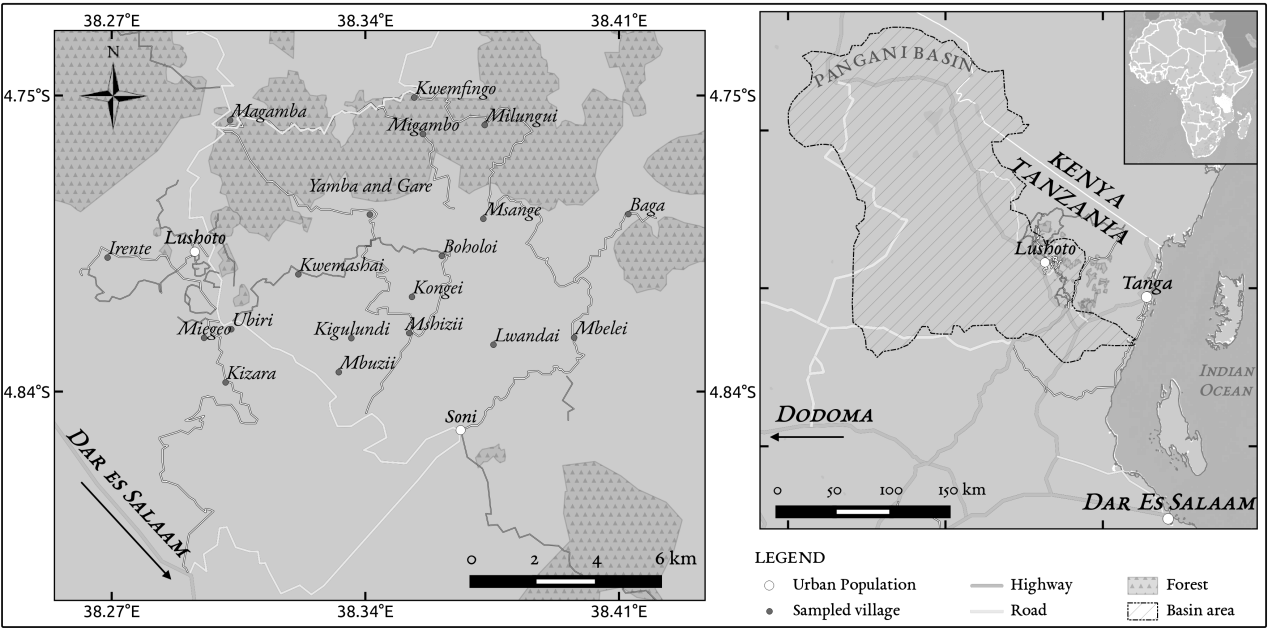
\includegraphics[width=0.9\textwidth]{figs_04/image1.png}
  \captionsetup{singlelinecheck = false, justification=justified} %left justify caption
  \caption{Study area, market infrastructure and environmental interactions}
  \label{map:04_1}
  %\small
  %\raggedright
  \vspace*{-3mm}
  \caption*{(Authors' composition based on GADM database and Open Street Maps)}
\end{figure}




The Usambara massif is densely populated by three ethnic communities: The Shambaa, Pare and Mbugu peoples (\citealp{Lyamchai2011}). Tribal social networks are still important but have become less distinctive in contemporary society, often secondary to family and religious networks (Islam and Christianity). A unique element of the culture and history in the Usambara highlands related to food security and soil conservation is that ``Access to unimproved subsistence land ... was still accepted as every resident's right... right up until the end of 1988'' (\citealp{Feierman1990}, p. 183). Modern livelihoods are largely based on agriculture and micro-enterprises, with some garnering formal employment, and others migrating to urban centres. In the villages of interest to this study, households generally have small land-holdings with a high dependency on agriculture (\citealp{Lyamchai2011}).

Several development activities have focused their efforts on the Usambara highlands, including projects on dairy, potatoes, sweet potatoes, forestry and bee-keeping. Three agricultural interventions were implemented at the time of this study (excluding forestry). One project released new bean varieties suited to the region (\citealp{Kimeli2014}); the second project trialled new potato varieties and provided farmer training on cultivation and value-chains in one of the study site's villages (namely Boheloi; \citealp{Harahagazwe2016}; \citealp{Harahagazwe2014}); the third project on dairy development, established trial plots of cultivated fodder, facilitated village level planning and worked to improve value-chain linkages. This dairy oriented project was implemented in four villages in the study site (namely Mbuzii, Ubiri, Kwemashai, Lwandai; \citealp{Kilelu20171102}). Government initiatives at multiple levels have also been working towards extending and improving the standard of the road network, electrification grid, water supply system, medical facilities and schools.

\subsection{Data collection}

Households in the study area were originally interviewed in July 2012. Data collection in 2012 was part of the Africa and South-East Asia wide CCAFS project, IMPACTlite. In Lushoto district, 200 households were sampled for IMPACTlite, being 10 households per village in a multi-stage clustered sampling design. Households were sampled based on a random geographic distribution of points within village boundaries -- as detailed in \citet{Rufino2013}. The survey was designed to collect details on farm inputs/outputs, farm activities, labour allocation, asset ownership, income and food security over a one year period. The survey's purpose was to be able to represent within site variability of livelihood indicators and provide insights into key performance indicators in terms of farm performance, food security, and the environment (\citealp{Rufino2013}).

In June-July 2015 a total of 147 households were re-sampled, with random selection at the village level resulting in six to eight households per village. Not all 200 households from 2012 were re-sampled; sampling in 2012 was more conservative as there was more uncertainty about variation between households in the site. The Rural Household Multi-Indicator Survey (RHOMIS) was utilised to represent livelihood strategies and some temporally consistent performance indicators (namely: food availability and household diet diversity). The RHOMIS tool evolved out of the IMPACTlite tool and has been designed to collect reliable information at minimum burden on respondents, providing a rapid characterisation of farm systems and performance indicators (\citealp{Hammond2017225}). This revised tool was used instead of the original IMPACTlite survey, as it collected information relevant only to a clear set of research questions and thus kept the burden to the farmer at a minimum. Interviews were conducted in Swahili and local tribal dialects by three trained enumerators and to a lesser extent by the first author. Enumerators differed from 2012, but the original site coordinator was closely engaged and worked with the enumerators in the study site to improve consistency and reduce biases that could be introduced by the way questions were phrased.

Village leaders and extension officers were interviewed concurrently to the household level interviews; in total 16 village level interviews were conducted. Topics of discussion included: changes in population, changes in land size, the importance of particular crops/livestock, livestock productivity, the condition of infrastructure and development activities (local, government or NGO led).

Additionally, insights were drawn from publicly available remote sensing products, namely: the `global satellite rain gauge', vegetative index and estimated soil properties.

\subsection{Analysis}

Using the paired observations over 2012 and 2015, this study analyses the financial and food security performance of differing adaptive responses for 147 households (thus excluding 53 out of the 200 households sampled in 2012). Changes between 2012 and 2015 were first assessed at the aggregate level. Summaries of the central tendency and distribution of households were provided for variables related to resource endowments (e.g. land, livestock and off-farm income), farm characteristics and performance indicators. As several variables of interest were not normally distributed, the central tendency was represented by the median and the distribution as the inter-quartile range (IQR).

Following on from analysis at the aggregate level, a hierarchical K-means clustering algorithm (\citealp{Kassambara2016}) then incorporated variables that would differentiate households in terms of long-term (strategic) and short-term (tactical) configurations of resources and farm characteristics -- termed `adaptive responses'. Variables included were: household population (in adult equivalents), total land cultivated, crop market participation (percentage of crop production sold), crop diversity (number of different crops grown), importance of high value crops (percentage of the area grown), crop-livestock integration (manure and crop residue utilisation), livestock-holdings and livestock market participation (percentage of livestock products sold) and off-farm income. Off-farm income was collected differently in 2012 and 2015. To maintain consistency, only income from business and employment was included, which was then evaluated as a percentage of total income. Market participation was assessed on a kilo-calorie basis (\% sold), providing a common unit of comparison across crops and livestock products. The final inputs into the clustering algorithm included the variables listed above from 2015 as well as the difference between 2015 and 2012 for each variable, all of which were centred and scaled.

Food security and poverty indicators were calculated using standardised methodologies as described in \citet{Hammond2017225}. The `household diet diversity score' (HDDS) is based on a count of a total of 12 food groups consumed (\citealp{Swindale2006}) with recall of `flush' and `lean' periods. The `household food insecurity access scale' (HFIAS) is based on nine questions on the household's experience of food insecurity for the flush and lean periods; touching on sensitive issues for the respondents such as missed meals and consumption of undesirable foods (\citealp{Coates2007}). The progress out of poverty index (PPI) is based on a country-specific set of 10 questions, scoring households from 0 to 100 (with higher scores increasingly less likely to be below the poverty line; Grameen, n.d.). Food availability is a supply and purchase potential estimate based on production, off-farm income and cost of a key staple food (maize; \textit{Zea mays L.}), expressed as Potential Food Equivalent (PFE) energy (kilocalories) per adult equivalent per day; a common calorie content was taken over the time period, with varying staple food price. It should be noted that the purchase potential from farm income has limitations as it is based on revenue rather than profit. Thus, food availability is calculated as follows (Eq. 4.1) and further detailed in \citet{Frelat2016458}.

\begin{equation}
\tag{4.1}
PFE = \frac{E_{cons} + E_{income}}{365 \times n_{hh}}
\end{equation}
%PFE = \textbackslash frac\{E\_\{cons\} + E\_\{income\}\}\{365 \textbackslash times n\_\{hh\}\} \textbf{(1)}

Remotely sensed products were used as explanatory variables for differences between years and clusters. Estimated monthly rainfall for the study site was used to identify variations from long-term average rainfall across the site as a whole (\citealp{Janowiak1999}). Additionally, the enhanced vegetative index (EVI; NASA, n.d.), soil organic carbon (SOC) and pH estimates were extracted for the households where reliable GPS coordinates were collected (n=78 due to GPS errors; estimation of soil properties detailed in \citealp{Hengl2016}). These products were at a 250 m resolution, as such these data represent approximate metrics for rainfall, temperature and soil for the farm and surrounds.

To account for the multi-stage clustered sampling design, changes over time and differences between clusters were modelled with mixed-effects regression, with random effects on the intercept from the village. Changes and differences in land, livestock holdings, income, fertiliser, food availability and food security of access were analysed using linear regressions; differences in HDDS between clusters were analysed using negative binomial regressions. All linear and negative binomial regressions were performed using the lme4 package in R (\citealp{BatesD2017}). Linear regressions with non-parametric residuals were re-run with cuberoot transformed dependent variables. The statistical significance of fixed effects in linear regressions were assessed using the F-test with Kenward-Roger approximation (\citealp{Kenward1997}), comparing models additively from the intercept only model. The statistical significance of fixed effects in negative binomial regressions were assessed using the wald test using the aod package in R (\citealp{Lesnoff2012}).

\section{Results}

\subsection{Summary of resources, farm characteristics and performance indicators}

Resources and farm characteristics were highly variable between households, both in 2012 and 2015 (Table \ref{tab:04_1}). While highly variable, these results support previous characterisations of the study site. Households generally have small land-holdings (85\% of households {\textless} 1.5 ha in 2015) with agricultural based livelihoods (87\% of households {\textgreater} half of their income coming from the farm in 2015) and a low level of input (88\% of households applying less than 15 kg of fertiliser ha$^{-1}$ year$^{-1}$). Results from the village level interviews indicated that agricultural development programs were implemented in five of the villages. Additional to these development programs, 12\% of households (from a total of 12 villages) received aid in the form of seed, fertiliser, food or money.




\begin{sidewaystable}
  \captionsetup{singlelinecheck = false, justification=justified} %left justify caption
  \caption{
  Resources, farm characteristics and performance indicators of households interviewed in 2012 and 2015 (median, IQR; n = 147)
  }
  \small
  \label{tab:04_1}
\begin{tabularx}{\textwidth}{@{}llYY@{}}
  %{
%p{\dimexpr 0.11\linewidth-2\tabcolsep}
%p{\dimexpr 0.57\linewidth-2\tabcolsep}
%p{\dimexpr 0.16\linewidth-2\tabcolsep}
%p{\dimexpr 0.16\linewidth-2\tabcolsep}}
\toprule
 Domain & Variable & 2012 & 2015 \\
 \midrule
\multirow{5}{*}{Resources} & Household members (adult equivalents) & 3.68 (1.70) & 3.60 (2.00) \\
 & Land owned (ha) & 0.7 (0.5) & 0.8 (0.8) \\
 & Land cultivated (ha) & 0.7 (0.5) & 0.8 (0.8) \\
 & Livestock (TLUs)$^{\mathrm{a}}$ & 1.04 (1.79) & 1.25 (2.30) \\
 & Off-farm income (\% total) & 0 (55) & 0 (3) \\
 \arrayrulecolor{black!30}\midrule
\multirow{5}{*}{Farm characteristics} & Crop diversity (Number of crops) & 4 (3) & 3 (2) \\
 & Crop market participation (\% of calories produced) & 25 (35) & 22 (43) \\
 & Livestock diversity (number of species) & 2 (1) & 2 (1) \\
 & Livestock market participation (\% of calories produced) & 0 (51) & 0 (6) \\
 & Fertiliser application (kg ha$^{-1}$) & 2 (46) & 3 (7) \\
 \arrayrulecolor{black!30}\midrule
\multirow{7}{*}{Performance indicators} & HDDS -- flush period$^{\mathrm{b}}$ & 3 (1) & 9 (3) \\
 & HDDS -- lean period$^{\mathrm{b}}$ & 3 (1) & 5 (3) \\
 & HDDS --\%age purchased & 75 (21) & 50 (31) \\
 & Food availability (kcal adult equivalent$^{-1}$ day$^{-1}$)$^{\mathrm{c}}$ & 3764 (5953) & 1831 (2590) \\
 & Maize yield (kg ha$^{-1}$) & 148 (161) & 543 (761) \\
 & Crop income (USD household$^{-1}$ year$^{-1}$)$^{\mathrm{d}}$ & 84 (152) & 56 (202) \\
 & Livestock income (USD household$^{-1}$ year$^{-1}$)$^{\mathrm{c,d}}$ & 0 (3) & 0 (0) \\
\arrayrulecolor{black}\bottomrule
\end{tabularx}
\footnotesize
\raggedright
%\caption*{
$^{a}$Adult cattle = 1, calves = 0.38, pigs = 0.3, sheep and goats = 0.2, chickens = 0.01. \\
$^{b}$Apparent changes between years may be explained by differences in survey design, respondent and/or enumerator.\\
$^{c}$Excluding live animal sales.\\
$^{d}$1 TSH = 0.00046 USD.%}
\end{sidewaystable}



Over the observed period there were statistically significant changes in the distribution of land ownership, crop diversity (pr(\textgreater{\textbar}F{\textbar}) {\textless} 0.01) and crop income (pr(\textgreater{\textbar}F{\textbar}) {\textless} 0.05, Appendix Table \ref{tab:A_1}). Between 2012 and 2015 some households aggregated land and others reduced land-holdings, flattening the overall distribution of land ownership in 2015 (Figure \ref{fig:04_1} a; pr {\textless} 0.01, F-test of variance). There were no statistically significant differences in livestock or off-farm income between 2012 and 2015.

\begin{figure}[H] %Change fig. hectares owned - land owned (ha)
  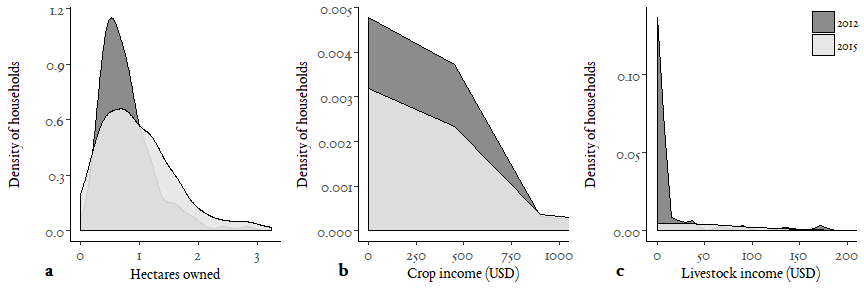
\includegraphics[width=1\textwidth]{figs_04/image2.png}
  \captionsetup{singlelinecheck = off, justification=justified}
    \caption{Distributions in 2012 and 2015 (a) Land owned (ha); b) Crop income (USD year$^{-1}$); c) Livestock income (USD year$^{-1}$)}
    \label{fig:04_1}
\end{figure}

Annual crop income was significantly lower in 2015; this was weakly related to changes in crop market orientation ($\hat{\alpha}$ = 64 (47), $\hat{\beta}$ = 394 (112) pr(\textgreater{\textbar}F{\textbar}) {\textless} 0.001, mixed-effects linear regression; Figure \ref{fig:04_2}), where some households decreased market participation and also decreased crop income, and others either remained stable or increased market participation and increased crop income.

There was no significant difference in vegetative index (EVI) between 2012, 2015 and the long-term annual average. Estimated rainfall, however, was more erratic in 2011 -- 2012, with approximately 90 mm more than average falling in November 2011 and approximately 90 mm less than average falling in May 2012. The most influential drought events (in terms of recorded crop yields), were recorded in both April 2011 (-100 mm) and April 2014 (-90mm), potentially influencing the main harvest recorded for each year (August 2011 and 2014; \citealp{Janowiak1999}). The effects of these rainfall differences are uncertain; harvests in 2012 may have been greater from the short rain planting period in 2011 (September -- November) and reduced for the long rain planting period in 2012 (February -- April).

\begin{figure}[H]
  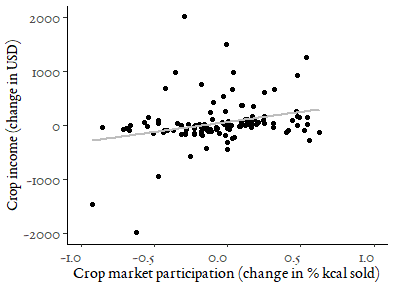
\includegraphics[width=0.6\textwidth]{figs_04/image3.png}
\captionsetup{singlelinecheck = off, justification=justified}
  \caption{Change in crop income (USD) and market participation (\% kcal sold), with regression line}
  \label{fig:04_2}
\end{figure}

The majority ({\textgreater}70\%) of households either did not have off-farm income opportunities or only earned a small proportion of their income from off-farm activities. In 2015, 3\% of households earned over 50\% of their income from off-farm activities, which is in contrast to 29\% of households in 2012. This change in off-farm income has no obvious explanation, but may indicate a lack of job security and a high risk of failure for off-farm businesses.

Observing these resources and farm characteristics over time, a diversity of concurrent changes are evident for a majority of households. Seventeen percent of households had a change in land area owned (${\pm}$ 1 ha). Seventy-seven percent of farmers show a change in land area owned, number of TLUs (${\pm}$ 2), market orientation of crops (${\pm}$ 50\%), market orientation of livestock (${\pm}$ 50\%), or changed crop diversity (${\pm}$ 2).

\subsection{Types of adaptive responses}

Four distinct groups were identified from the clustering process. Adaptive response clusters were named: `Rising high value crop' (n=25), `Rising livestock' (n=33), `Subsisting mixed' (n=42), and `Subsisting crops' (n=47; Table \ref{tab:04_2}).

Households in the `Rising high value crop' cluster were named based on their increased land area (64\% of households increased by {\textgreater} 0.25 ha), a larger allocation of land to non-staple crops (92\% of households), and their increased crop market participation. Increases in land area were allocated to tomatoes (29\% of households that increased land), potatoes (17\% of households) and coffee (16\% of households). Households in this cluster continued to cultivate staple crops, maintaining their high level of crop diversity over the three year period. Several households in this cluster also increased their livestock-holdings (predominantly cattle); the majority (73\%), however, reduced their market participation of livestock products. Twenty-four percent of households earned off-farm income in 2015, considerably less than the 56\% of households earning in 2012. Increases in land ownership indicate a shift in strategy for households in this cluster. While cultivating staple crops has been a consistent aspect of their farm strategy, cultivating high value crops may be a long-term strategy for some (e.g. 28\% of households had coffee bushes in 2012 and 2015), or a short-term tactic for others (e.g. 68\% of households added high value crops to their production mix in 2015).

Households in the `Rising livestock' cluster were named based on their increased land area (66\% increasing by {\textgreater} 0.25 ha), increased livestock-holdings (90\% of households) and their recent livestock market participation. These households also increased their cultivation and market participation of staple crops and cultivated a small portion of high value vegetables. Increases in land area were allocated to maize (60\% of households that increased land) and to a lesser extent increases in potatoes or tomatoes (14\%). Households that increased livestock-holdings generally did so by increasing cattle numbers (the majority of which were cross-bred or `exotic'), with a few exceptions of increased sheep and goat numbers. Livestock products were predominantly used for home consumption in both 2012 and 2015. Market participation of livestock products was not common in 2012; in 2015, however, 45\% of households in this cluster sold milk, eggs or home butchered meat. Live animals were marketed by the majority of households (51\%). Off-farm income was also earned by the majority of households (51\%) in 2015, ranging from 25 to 70\% of total income.

Households in the `Rising livestock' cluster sold live animals and increased livestock-holdings, indicating a viable long-term strategy, rather than short-term tactical destocking. The ownership of higher value mixed or `exotic' breeds (56\% of households) may also indicate a long-term strategy. Marketing of livestock products, however, may be a strategy for some (e.g. 15\% of households kept non-local cattle and marketed milk in 2015) and a tactic for others.

Households in the `Subsisting mixed' cluster, in general, maintained land-holdings, increased the portion of their land dedicated to staples and increased livestock-holdings. Crop and livestock market orientation decreased considerably when compared to 2012. The majority (65\%) of households kept cattle in 2012 and 2015, largely for home consumed milk production in 2015. Cattle keeping in the context of these communities is a considerable investment with barriers to procurement and sale; these households appear to be acting strategically on their asset ownership but may act tactically on whether to sell their milk or not.

Households in the `Subsisting crop' cluster reduced land cultivation, reduced crop market orientation and reduced livestock-holdings. The majority (91\%) kept poultry in both 2012 and 2015 indicating that livestock plays an important tactical role in this cluster; several households (29\%) ceased to keep cattle in 2015, indicating a potential strategic change.



\begin{sidewaystable}
  \captionsetup{singlelinecheck = false, justification=justified} %left justify caption
  \caption{
  Clustering variables by adaptive response cluster in 2012 and 2015 (median, IQR)
  }
  \label{tab:04_2}
  \small
%\begin{tabularx}{\textwidth}{@{}lYYYYYYYYYY@{}}
%  {
%p{\dimexpr 0.19\linewidth-2\tabcolsep}
%p{\dimexpr 0.09\linewidth-2\tabcolsep}
%p{\dimexpr 0.08\linewidth-2\tabcolsep}
%p{\dimexpr 0.07\linewidth-2\tabcolsep}
%p{\dimexpr 0.08\linewidth-2\tabcolsep}
%p{\dimexpr 0.08\linewidth-2\tabcolsep}
%p{\dimexpr 0.08\linewidth-2\tabcolsep}
%p{\dimexpr 0.08\linewidth-2\tabcolsep}
%p{\dimexpr 0.08\linewidth-2\tabcolsep}
%p{\dimexpr 0.09\linewidth-2\tabcolsep}
%p{\dimexpr 0.09\linewidth-2\tabcolsep}}
\begin{tabular}{L{3.8cm}cccccccc}
\toprule
 & \multicolumn{2}{C{3.6cm}}{\makecell{Rising high value crop \\ (n=25)}} & \multicolumn{2}{C{3.6cm}}{\makecell{Rising livestock \\ (n=33)}} & \multicolumn{2}{C{3.6cm}}{\makecell{Subsisting mixed \\ (n=42)}} & \multicolumn{2}{C{3.6cm}}{\makecell{Subsisting crop \\ (n=47)}} \\
 \cmidrule{2-9}
 & 2012 & 2015 & 2012 & 2015 & 2012 & 2015 & 2012 & 2015  \\
 \midrule
Household population (adult equivalents) & 3.84 (1.33) & 4.05 (2.3) & 3.81 (1.7) & 4.3 (1.8) & 3.88 (1.89) & 3.8 (1.44) & 3.3 (1.39) & 2.6 (1.62)  \\
Land owned (ha) & 0.71 (0.60) & 1.21 (0.81) & 0.71 (0.20) & 1.21 (0.81) & 0.71 (0.58) & 0.61 (0.81) & 0.61 (0.56) & 0.81 (0.81)  \\
Land cultivated (ha) & 0.71 (0.50) & 1.11 (0.81) & 0.71 (0.20) & 1.21 (0.81) & 0.71 (0.58) & 0.61 (0.49) & 0.61 (0.56) & 0.40 (0.41)  \\
Crop market participation$^{\mathrm{a}}$ & 30 (32) & 39 (23) & 23 (30) & 34 (38) & 29 (31) & 16 (30) & 19 (41) & 0 (25) \\
Crop diversity & 4 (3) & 4 (2) & 4 (3) & 4 (1) & 5 (2) & 3 (1) & 3 (3) & 2 (1)  \\
High value crops$^{\mathrm{b}}$ & 0 (9) & 22 (13) & 0 (10) & 0 (8) & 0 (4) & 0 (0) & 0 (0) & 0 (0)  \\
Livestock (TLUs) & 1.08 (1.85) & 1.9 (1.40) & 1 (1.39) & 2.91 (2.30) & 1.28 (1.24) & 1.82 (1.25) & 0.16 (1.40) & 0.05 (0.45) \\
Livestock market participation$^{\mathrm{a}}$ & 40 (75) & 0 (30) & 0 (0) & 0 (34) & 0 (73) & 0 (1) & 0 (0) & 0 (0) \\
Crop-livestock integration (\% practices) & 50 (50) & 100 (0) & 50 (50) & 100 (0) & 50 (0) & 100 (0) & 0 (50) & 50 (25) \\
Off-farm income (\% total) & 16 (52) & 0 (0) & 12 (73) & 25 (50) & 0 (26) & 0 (0) & 0 (46) & 0 (0)  \\
\bottomrule
\end{tabular}
\footnotesize
\raggedright
%\caption*{
\\
$^{a}$ Percent of calories produced.\\
$^{b}$ Percent of area cultivated. \\%}
\end{sidewaystable}




\subsection{Analysis of adaptive responses}

A range of non-clustering variables were considered as potential covariate attributes of the clusters. These included: gender of the household head, whether the household head changed, household structure (e.g. tri-generational, parent-child, individuals), aid (seed, fertiliser, food and financial), distance of plot (from homestead), fertiliser application, debt, elevation, SOC, soil acidity and average EVI in 2012 and 2015.

The gender of household head was significantly different between clusters ($\hat{\alpha}$ = -1.63 (0.30, $\hat{\beta}$ = 1.77 (0.44) pr(\textgreater{\textbar}{\chi}$^2${\textbar}) {\textless} 0.05, mixed-effects logistic regression, reference categories -- male head and non-`Subsisting crops'), with `Subsisting crops' having the highest instance of female-headed households (53\% of households), followed by `Subsisting mixed' (26\% of households). The gender and marital status of the household head can have land tenure implications, as well as implications on livestock ownership. In this case, there were significant differences in the full data set, with female heads cultivating less land than their male counterparts (pr(\textgreater{\textbar}F{\textbar}) {\textless} 0.001, Appendix Table \ref{tab:A_2}); and, female heads owning less livestock assets in 2015 (TLU; pr(\textgreater{\textbar}F{\textbar}) {\textless} 0.001, Appendix Table \ref{tab:A_2}). Within the `Subsisting' clusters, however, there were no differences between male and female heads in terms of land-holdings. In the `Subsisting mixed' cluster, male-headed households had significantly higher livestock-holdings (particularly cattle; pr(\textgreater{\textbar}F{\textbar}) {\textless} 0.05, Appendix A Table \ref{tab:A_3}).

Spatial analysis of a digital elevation model and soil property estimates (\citealp{Hengl2016}) of the study area showed that elevation was negatively correlated with pH and positively correlated SOC (r = -0.61, pr {\textless} 0.05; r = 0.79, pr {\textless} 0.01, Pearson's correlation). Despite this spatial variability, the modelled acidity and SOC levels would not present significant differences in crop or pasture constraints between clusters (e.g. pH was between 5.3 and 6.2 and optimal pH for maize in a nutrient solution is between 5.2 and 6.5; \citealp{Islam1980339}). It should be noted, however, that non-publicly available, finer scale modelling of the study area suggests that there is greater variability and instances of lower SOC than available at a 250 m resolution (compared to \citealp{Winowiecki2016263}).

Households in `Rising' clusters applied significantly more synthetic fertiliser per hectare in 2015 when compared to `Subsisting' households ($\hat{\alpha}$ = 3.85 (2.43), $\hat{\beta}$ = 8.98 (3.59) pr(\textgreater{\textbar}F{\textbar}) {\textless} 0.05, mixed-effects linear regression). Manure was often applied along with synthetic fertilisers, particularly for potatoes in `Rising' clusters and the `Subsisting mixed' households, as well as tomatoes and other vegetables in `Rising high value crops' households. Yields were significantly higher for households applying synthetic fertilisers to maize ($\hat{\alpha}$ = 719 (212), $\hat{\beta}$ = 813 (288) pr(\textgreater{\textbar}F{\textbar}) {\textless} 0.01, mixed-effects linear regression).

There was no statistically significant difference in receipt of aid, level of debt, distance of plot, household structure or EVI. Further, households in villages with ongoing interventions (potato and dairy) did not increase in scale or market orientation for those livelihood activities more than households in other villages.

\subsection{Outcomes of adaptive responses}

The distribution of crop incomes changed over time for all clusters, with median income increasing in `Rising' clusters and decreasing in `Subsisting' clusters (Figure \ref{fig:04_3}; $\hat{\alpha}$ = 7.57 (0.77), $\hat{\beta}$ = -4.30 (1.21) pr(\textgreater{\textbar}F{\textbar}) {\textless} 0.01, mixed-effects linear regression). The increased crop income in the `Rising high value crop' cluster was attributable to market vegetables such as tomatoes, rather than coffee which halved in price between 2012 and 2015.

\begin{figure}[H]
  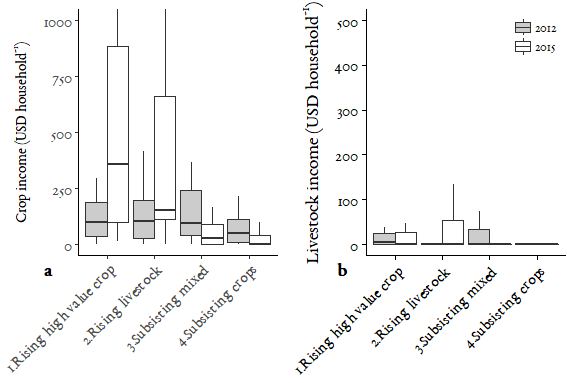
\includegraphics[width=0.6\textwidth]{figs_04/image4.png}
  \captionsetup{singlelinecheck = off, justification=justified}
    \caption{a) crop income (USD household$^{-1}$) by adaptive response cluster b) Livestock income performance (USD household$^{-1}$) by cluster}
    \label{fig:04_3}
\end{figure}
\vspace*{-3mm}

The distribution of livestock incomes did not differ significantly between 2012 and 2015. However, fresh milk producers in the `Rising' clusters generated significantly higher livestock incomes when compared to other households in the cluster ($\hat{\alpha}$ = 1.46 (0.36), $\hat{\beta}$ = 0.92 (0.40) pr(\textgreater{\textbar}F{\textbar}) {\textless} 0.01).

Households in the `Rising' clusters had significantly higher Food Availability scores and Household Diet Diversity Scores in the good period when compared to `Subsisting' clusters (Figure \ref{fig:04_4}; pr(\textgreater{\textbar}F{\textbar}) {\textless} 0.001, Appendix Table \ref{tab:A_4}).

In the lean period, `Subsisting crops' households had significantly less diverse diets than `Rising livestock' households ($\hat{\alpha}$ = 1.57 (0.07), $\hat{\beta}$ = 0.21 (0.10) pr(\textgreater{\textbar}{\chi}$^2${\textbar}) {\textless} 0.05, mixed-effects negative binomial regression). Households in the `Rising' clusters were significantly more food secure (in terms of access) than `Subsisting' households ($\hat{\alpha}$ = 9.48 (0.61), $\hat{\beta}$ = -2.28 (0.80) pr(\textgreater{\textbar}F{\textbar}) {\textless} 0.01, mixed-effects linear regression).

There was no significant difference in the PPI score; this is understandable as PPI is a slower moving indicator, requiring more time to see significant differences in performance.

Notably, there was no significant difference between clusters in the duration of the lean period (median = 3, IQR = 1), indicating that the pertinent issue is the intensity of hardship, rather than duration. Further, there was no significant difference in performance due to aid or gender of household head (results not shown).

\begin{figure}[H]
  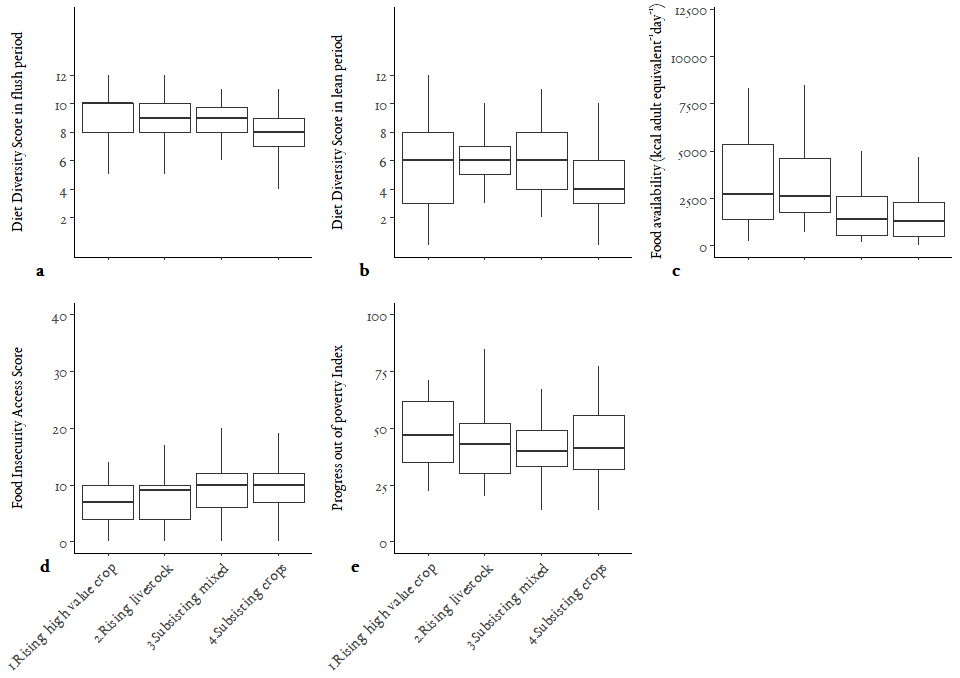
\includegraphics[width=1\textwidth]{figs_04/image5.png}
  \captionsetup{singlelinecheck = off, justification=justified}
    \caption{Performance indicators by adaptive response cluster in 2015. (a) Household diet diversity scores (HDDS) in the flush period; (b) Household diet diversity dcores in the lean period; (c) Food availability (kcal adult equivalent$^{-1}$ day$^{-1}$), including live animal sales; (d) Household food insecurity access scale (HFIAS); (e) Progress out of poverty index score}
    \label{fig:04_4}
  %\small
  %\raggedright

\end{figure}
\vspace*{-3mm}

\section{Discussion}

Households in the study site responded to local and national circumstances (e.g. drought months, regional and national economic growth) through a range of adaptive responses which have been classified as `Rising high value crop', `Rising livestock', `Subsisting mixed' and `Subsisting crops' (summarised in Table \ref{tab:04_3}). Overall, within the relatively short time period of three years (2012 -- 2015), 77\% of households made changes in farm resources or farm characteristics (Figure \ref{fig:04_1}a and Table \ref{tab:04_2}). Many of these changes can be classified as strategic, requiring considerable investment which will have an influence on the performance of the farming system over a longer period of time (e.g. 17\% of households changing land area by {\textgreater} 1 ha). Other observed changes (increases in vegetable production, changes in off-farm income) are more difficult to identify as long-term strategic changes as opposed to short-term tactics. A consequence of these rapid changes is that agency interventions need to be adaptable to maintain relevance for such farmers. Our results show that in sites like Lushoto with a good rural to urban connection (such as can be found in several regions of sub-Saharan Africa due to the many rapidly developing urban centres) projects are indeed aiming for a moving target and this will have implications on achieving income and food security outcomes, and requires targeted and rapid monitoring tools. There are valuable lessons that can be learned from this case study for macro development activities in the region (e.g. providing infrastructure and stimulating off-farm industries) as well as micro development activities (e.g. targeting and designing agency interventions).


%Alternative for this table https://latex.org/forum/viewtopic.php?t=8674
\begin{sidewaystable}
\captionsetup{singlelinecheck = false, justification=justified} %left justify caption
  \caption{
  Summary of changes in farm characteristics by cluster
  }
  \small
		%\centering
  \label{tab:04_3}
\begin{tabularx}{\textwidth}{
p{\dimexpr 0.18\linewidth-2\tabcolsep}
p{\dimexpr 0.08\linewidth-2\tabcolsep}
p{\dimexpr 0.08\linewidth-2\tabcolsep}
p{\dimexpr 0.08\linewidth-2\tabcolsep}
p{\dimexpr 0.08\linewidth-2\tabcolsep}
p{\dimexpr 0.08\linewidth-2\tabcolsep}
p{\dimexpr 0.08\linewidth-2\tabcolsep}
p{\dimexpr 0.08\linewidth-2\tabcolsep}
p{\dimexpr 0.08\linewidth-2\tabcolsep}
p{\dimexpr 0.08\linewidth-2\tabcolsep}
p{\dimexpr 0.08\linewidth-2\tabcolsep}}
\toprule
 & Land owned & Livestock holdings & Staple crops (\% area) & High value crops (\% area) & Crops marketed & Crops subsistence & Dairy marketed & Dairy subsistence & Poultry subsistence & Live animals marketed \\
 \midrule
Rising high value crops & ${\uparrow}$ H & ${\uparrow}$ M & ${\downarrow}$ M & ${\uparrow}$ H & ${\uparrow}$ H & {\textbullet} M & {\textbullet} L & {\textbullet} M & {\textbullet} H & M \\
Rising livestock & ${\uparrow}$ H & ${\uparrow}$ H & ${\uparrow}$ H & {\textbullet} L & ${\uparrow}$ H & {\textbullet} M & ${\uparrow}$ M & {\textbullet} M & {\textbullet} H & H \\
Subsisting mixed & {\textbullet} L & ${\uparrow}$ M & {\textbullet} H & {\textbullet} L & ${\downarrow}$ M & {\textbullet} H & {\textbullet} L & {\textbullet} M & {\textbullet} M & M \\
Subsisting crops & {\textbullet} L & ${\downarrow}$ L & {\textbullet} H & {\textbullet} L & ${\downarrow}$ L & {\textbullet} H & {\textbullet} 0 & ${\downarrow}$ L & {\textbullet} H & L \\
\bottomrule
\end{tabularx}
\footnotesize
\raggedright
%\caption*{
${\uparrow}$Increase in the cluster between 2012 and 2015 ${\downarrow}$ decrease in the cluster; {\textbullet} no significant change in the cluster. \\
L low level exhibited in cluster 2015; M medium; H high; 0 characteristic was not present in cluster.%}

\end{sidewaystable}



Some of the most substantial changes we observed in the three year period of study were most likely not related to any of the agency interventions that were being promoted in the region. Increases in land area, for example, coincided with increases in the tomatoes, potatoes, maize and coffee plantings. While there was active promotion of potato cultivation in Boheloi, there were no households in this village that increased land area and potato cultivation, suggesting that this intervention is not, in part, driving this land aggregation. The role that dairy interventions have had in increased livestock-holdings is also not clear. Dairy is actively promoted (through the `Maziwa zaidi' project branding -- bringing multiple partners and projects under the one banner) in four of the villages; households in the `Rising livestock' cluster that increased milk marketing, however, are spread out across the study site and so it is difficult to definitively attribute these changes to this intervention program.

The change of land expansion seen in the `Rising' clusters provides a counterpoint to the trend established in the literature of decreasing farm sizes across lower-income countries more broadly, and specifically in Africa (\citealp{HLPE2013}; \citealp{Jayne2003253}; \citealp{Lowder201616}; \citealp{Masters2013156}). On a national scale, \citet{Jayne2014} found that average farm sizes in Tanzania, being land abundant, had more than doubled between 1996 and 2003, with increases in land value making parents less willing to subdivide. The conditions for such expansion though, go beyond land value and also relates to the business viability of the farm. The business viability of land expansion depends on the potential to gain economies of scale (\citealp{Hazell20101349}), viable market opportunities and effective risk management (\citealp{Harris2014}).

Our clusters of change show some similarity to Dorward's classification of farm livelihoods (\citealp{Dorward2009}). Our `Rising' clusters can be compared to the `Stepping-up' group of households and `Subsisting' households can be equated to the `Hanging-in' group (\citealp{Falconnier2015}; \citealp{Valbuena20151395}), but this study shows these rural households can pursue completely different strategies. In general terms, Dorward's livelihood grouping can be a useful framework. In specific applications like in this study, however, it is not the most appropriate way of looking at farm household trajectories.

In an assessment of food availability of more than thirteen thousand households in sub-Saharan Africa, \citet{Frelat2016458} make predictions using variables related to livelihoods, namely: household size, number of livestock and land area. Notional food availability though, as seen in this study, does not necessarily translate to improvements in all aspects of food security. Specifically, significant differences in food availability between clusters are not present in HFIAS and HDDS in the lean period (Figure \ref{fig:04_4}), suggesting that it is necessary to include multiple metrics of food security, rather than food availability alone.

\subsection{Farm income and food security in Lushoto, Tanzania}

Regardless of adaptive response, farmers utilise resources with a high level of production risk and with no guarantee that crops or animal-sourced foods will be purchased above cost, if at all. Households in the `Rising high value crops' and `Rising livestock' clusters had a high degree of market orientation, with different approaches to market risk (Table \ref{tab:04_2}). The `Rising high value crop' households' decisions appear to have been financially beneficial, by cultivating more land, with a portfolio of coffee, tomatoes, market vegetables, staples as well as keeping livestock species. It may well be that the increased risk of their expansion strategy was mitigated by an astute set of tactics in response to crop market signals while maintaining or increasing a diversity of crop and livestock species (rather than specialising). The `Rising livestock' households' focus on livestock and staple crops also returned financial dividends; this is particularly the case for fresh milk producers in the `Rising' clusters, who are earning significantly more livestock revenue than other households and could indicate greater specialisation for these households (as theorised would happen in such favourable market conditions in \citealp{McIntire1992}). These clusters of households demonstrate how agile and fast moving households in the study area can be.

The higher performing `Rising' adaptive response clusters also present a challenge for external organisations seeking to replicate such performance. The complex risk management and market responsiveness that manifests as a diversity of crop and livestock products in these adaptive response clusters is at odds with single focus activities that external organisations tend to promote (as illustrated by free seed not translating into food security or diet diversity performance); further, the land expansion that this strategy depends on for its performance is risky. This potentially represents a future of winners and losers, ultimately with some landholders falling further into poverty rather than leveraging their agricultural enterprises to improve their well-being.

Longer term resilience of land-holding households is not guaranteed. Higher performance or subsistence at the expense of the natural resource base can only be sustained for so long. Ongoing cultivation with minimal fallow and low inputs will work to deteriorate soil health in the future, limiting crop and pasture production. Households keeping ruminant livestock species (`Rising' and `Subsisting mixed') managed integrated crop-livestock systems, which is a positive attribute in terms of yields and soil health.

\section{Conclusions}

This study observes livelihood dynamics and related poverty and food security performance over a three year period in a high potential, market connected region of Tanzania. Evidence suggests that 1) the drivers for the most significant livelihood changes do not necessarily relate to agency interventions; 2) the adaptive responses that have been implemented in this community incorporate multiple components (e.g. off-farm income, diverse crops and livestock) and are relatively heterogeneous across the study site; and 3) there is a partial disconnect between potential food availability (from income and kcal production) and short and long-term food security. Such evidence has implications for development agendas.

A substantial portion of households in the study site made changes to their livelihoods over the short three-year period analysed in this paper. Changes in land ownership, livestock-holdings and high value crop production are most likely related to market opportunities and personal circumstances, rather than direct interventions. Several households are making substantial strategic changes by expanding land ownership, planting perennial crops and investing in exotic cattle breeds; many households are also tactically utilising their land for diversified, mixed crop-livestock production. The majority of households, however, have either remained stable or are scaling back to subsistence farming. Households that are expanding their land area, present a unique case study in sub-Saharan Africa, where households in land scarce regions (albeit in a land abundant country) are consolidating land, with the potential to gain economies of scale.

Government and non-government organisations face challenges in designing interventions that remain relevant to such rapidly changing rural households, with multifaceted livelihoods and varying `well-being priorities'. This study highlights, the need for interventions to simultaneously support a diversity of livelihood activities (e.g. dairy, staples and post-farm value chain) targeted at clusters of households. Monitoring of income and food availability is not sufficient to measure well-being, rather multiple well-being indicators are needed.

\section{Acknowledgements}

We thank all the people involved in the conversations that formed the basis for this study and especially the farmers for sharing their valuable time. We also thank the three anonymous reviewers for their comments and insights. This work is a joint output of the CGIAR Research Programs on `Livestock and Fish', `Climate Change, Agriculture and Food Security' (CCAFS) and `Maize'. The work was also supported by the USAID-funded Feed the Future Sustainable Intensification Innovation Laboratory. The views expressed in this paper can not be taken to reflect the official opinions of these organisations.

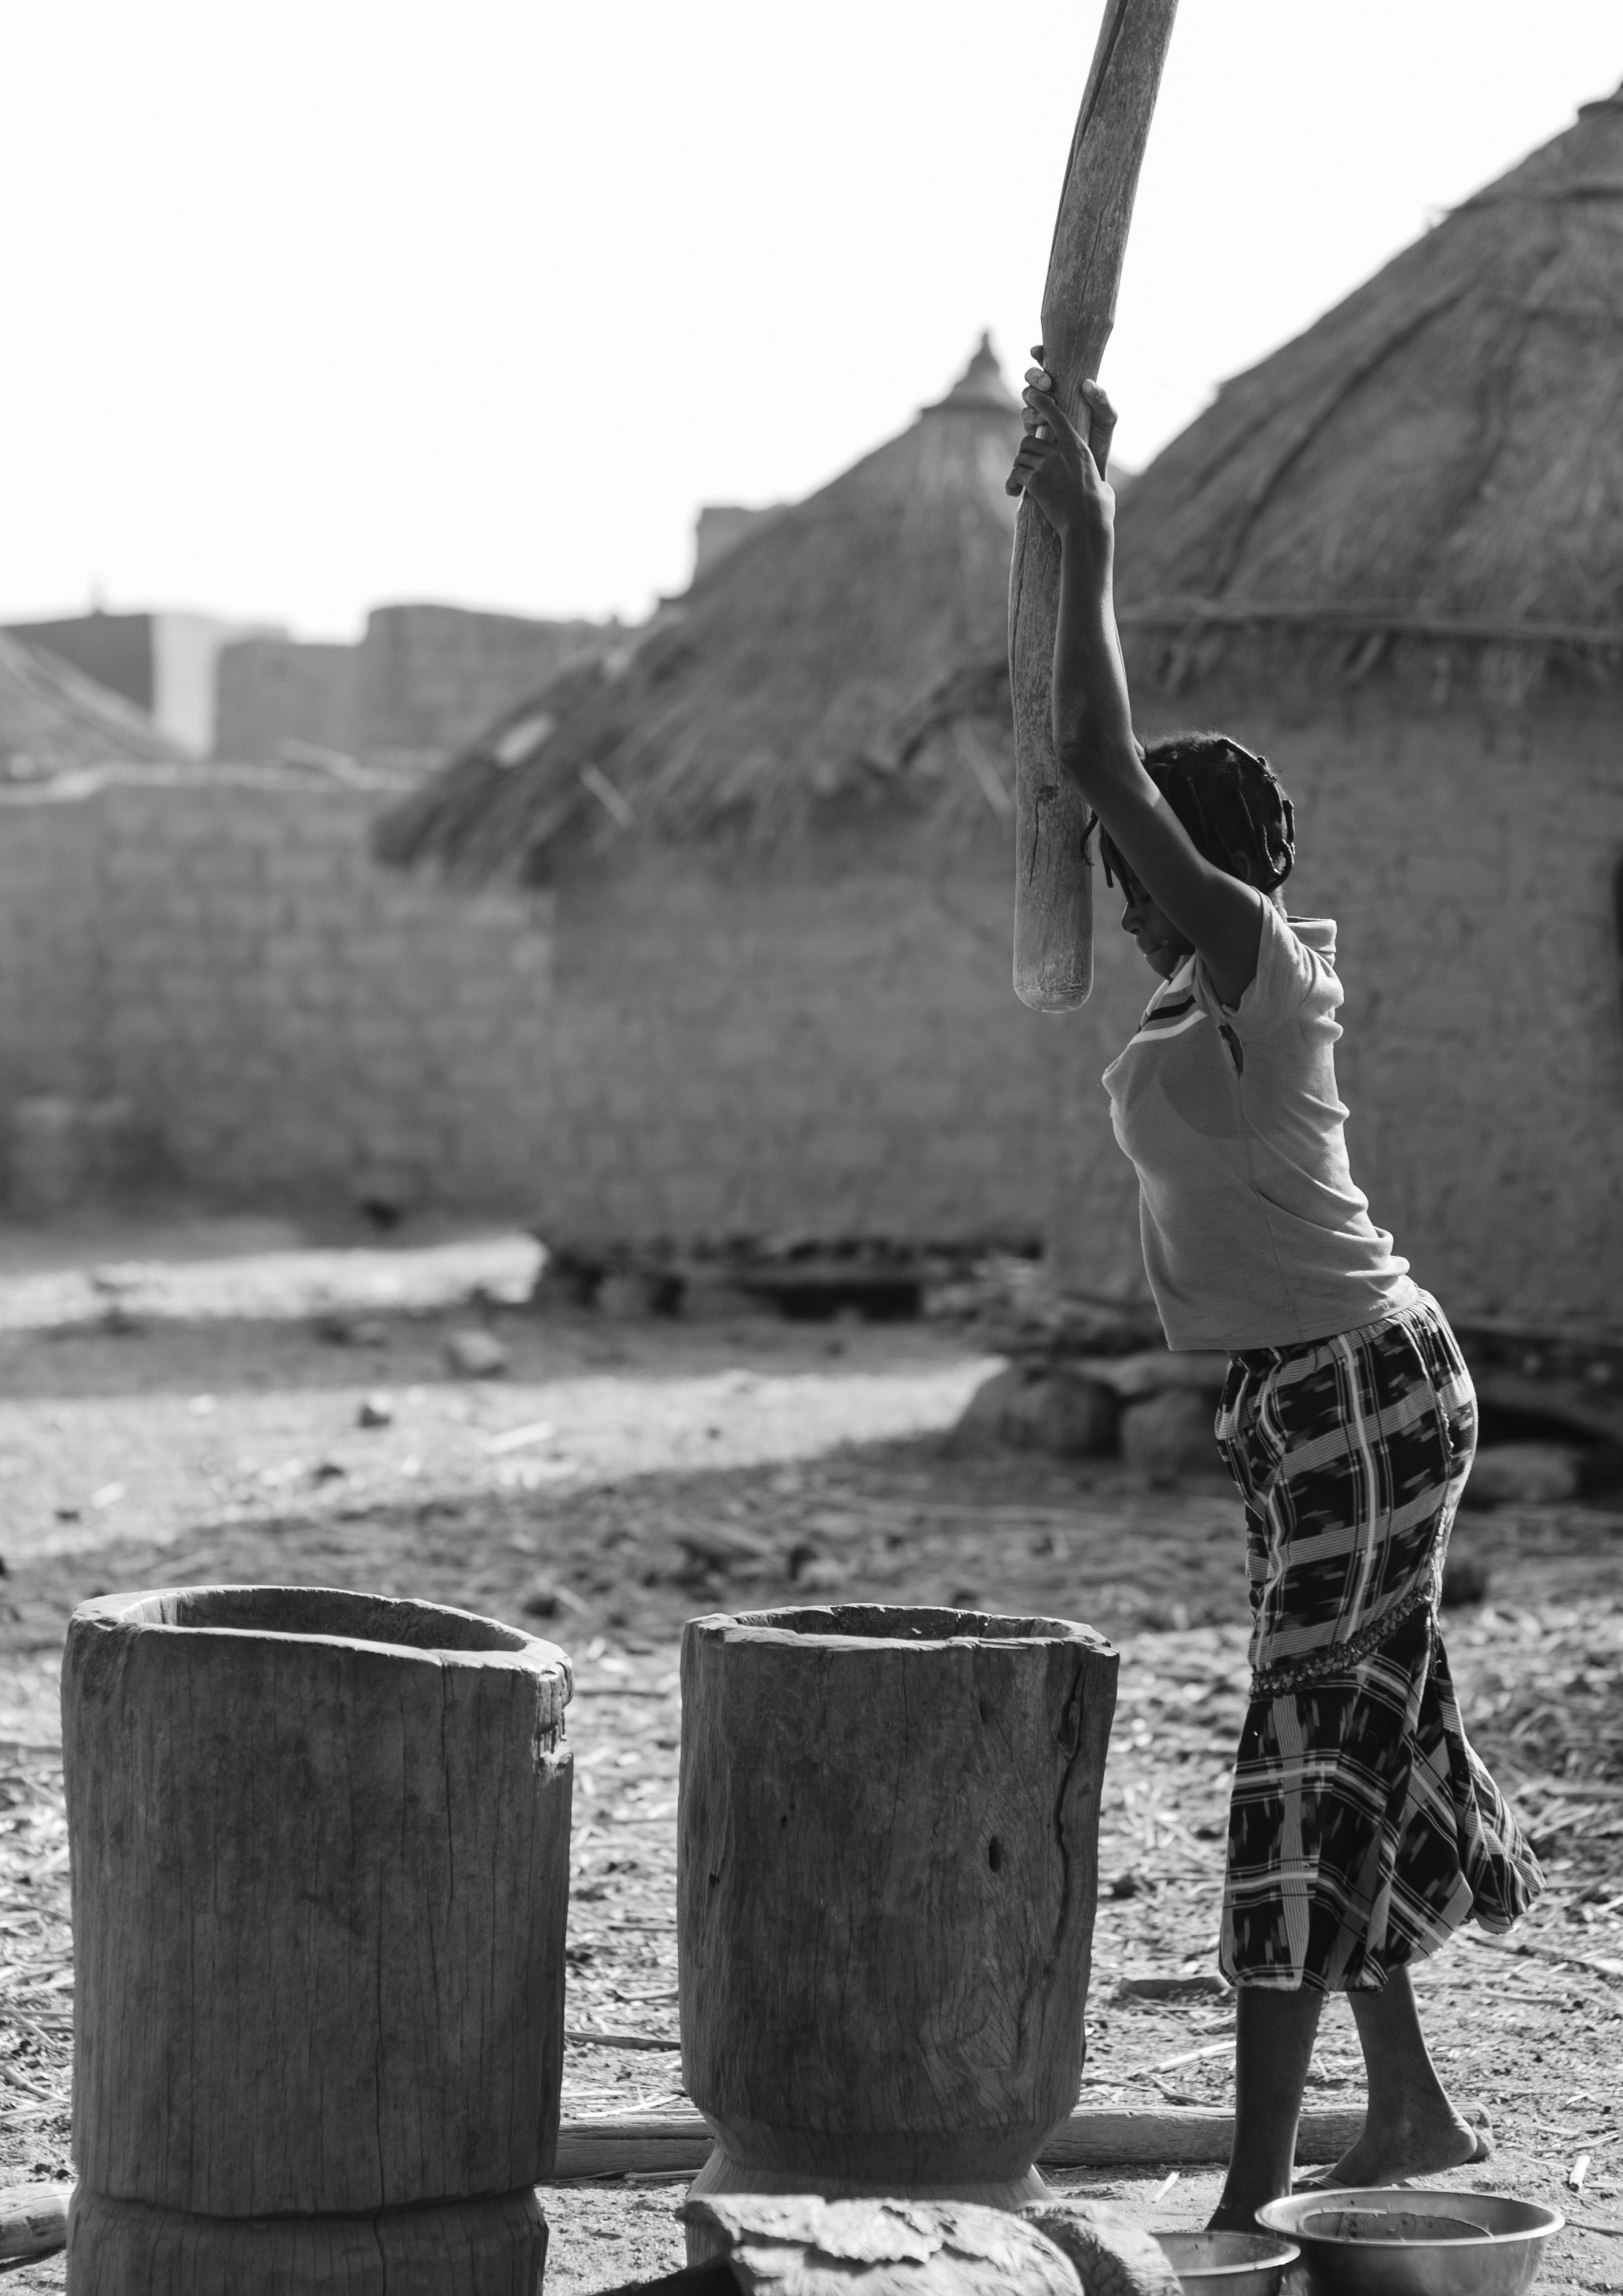
\includepdf{ChapterPics/Ch5Pound.JPG}
\chapter[Pathways to food security in rural Burkina Faso: the importance of consumption of home-produced food versus purchased food]{Pathways to food security in rural Burkina Faso: the importance of consumption of home-produced food versus purchased food} %TOC then chapter title
\chaptermark{Pathways to food security in rural Burkina Faso} %Running head
\label{cha:chapter5}
\vspace*{\fill}
This chapter is based on:
\\
\\
% Full citation of the published (or submitted/in review) article

Fraval, S., Yameogo, V., Ayantunde, A., Hammond, J., de Boer, I. J. M., Oosting, S. J., van Wijk, M. T. (submitted). \textit{Food Security}


\newpage

\section*{Abstract}
The number of undernourished people and the risk of micro-nutrient deficiency remains high in sub-Saharan Africa (SSA). Decades of policy designed to reverse the trends of food insecurity have illustrated that the causal pathways of intervention to end-point outcomes, such as nutrition, are not necessarily straightforward. Utilising well-established proxies for food security, this study investigates the relative importance of different pathways to food security in two subtly contrasting communities in the Sahelian and Sudanian Savanna zones of Burkina Faso (n=400). In Yatenga province, approximately 31\% of households were classified as `severely food insecure' in the `lean' period. In contrast, over 83\% of households sampled in Seno province were classified as being `severely food insecure' in the lean period. There were statistically significant associations between food security indicators and off-farm income, farm income and production diversity. The source of income had significantly different associations with diet diversity in the two provinces. In Yatenga province, higher gross farm income in the absence of off-farm income was predicted to result in more diverse diets; in Seno province, however, gross farm income was only predicted to result in more diverse diets when households are also earning off-farm income. Our analysis shows that, households are most differentiated by income generating pathways to food security. This finding should not detract from the essential role played by home-produced foods in improving food security. Rather, market-orientated agriculture and production for home consumption, as shown by households in this study, can be combined as part of a more resilient livelihood strategy.

\newpage

\section{Introduction}

The decade long decline in global chronic undernourishment has been reversed in recent years. The prevalence of chronic undernourishment in sub-Saharan Africa (SSA) has returned to pre-2005 levels, equating to approximately 237 million people unable to meet their energy needs in 2017 (\citealp{FAO2018}). There is also a high risk of micro-nutrient deficiency in the broader population, termed `hidden hunger' (another important aspect of malnutrition). \citet{Joy2014} provide startling estimates of deficiency risks for calcium ({\textgreater}50\% of the African population), zinc (40\%), selenium (28\%) and iodine (19\%). The individual and societal implications for such nutritional gaps are borne disproportionately by the rural population, indicated by the consistently higher prevalence of stunting in rural SSA (\citealp{Green2016}).

Given the persistence of undernourishment and hidden hunger, nutrition specific and nutrition sensitive interventions have been implemented across SSA (\citealp{DePee2017}). Agricultural interventions have an intuitive link with the most nutritionally vulnerable of communities, particularly those with limited off-farm employment options. The causal pathways from intervention to end-point outcomes, such as nutrition, are less straightforward (\citealp{Carletto2017}). Increased incomes and energy availability, for example, are necessary for alleviating undernourishment, but not sufficient for addressing `hidden hunger' (\citealp{Schipanski2016}; \citealp{McDermott2015}; \citealp{Hoddinott2012}). A greater understanding of these pathways is needed, particularly given the UN's ambitious target of `zero hunger' by 2030 (as part of the Sustainable Development Goals) with the constraints of stagnating aid flows (\citealp{OECD2015}) and low levels of research and development spending in SSA (\citealp{Pardey2016}).

One challenge in assessing the pathways from agricultural intervention to nutrition outcomes relates to monitoring the food security status of the population. Evaluating food access and micro-nutrient deficiencies has traditionally been time-consuming and invasive. More recently, however, proxies have been introduced to enable wide-scale monitoring and evaluation. Food insecurity scales and diet diversity scores (to a greater extent) have been assessed against diet quality and adequacy ratios, and have emerged as reliable proxies (evident in \citealp{Rah2010}; \citealp{Saha2009}; \citealp{Coates2007}; \citealp{Savy2005}; \citealp{Steyn2006}; \citealp{Arimond2004}; \citealp{Torheim2004}). In the one case where `household diet diversity score' (HDDS) was not associated with diet quality or adequacy ratios, an association was instead identified with `household food insecurity of access scale/prevalence' (HFIAS/HFIAP; \citealp{McDonald2015}). As HFIAS/HFIAP and HDDS represent different aspects of food security, both metrics are adopted in the present study.

Utilising these proxies for food insecurity, a growing body of literature has taken shape around the question of what differentiates those that are food insecure from those that are more food secure in high risk communities around the world. \citet{Powell2015} provides a summary of six such studies that identify positive relationships between the diversity of crops cultivated and HDDS. More recently, several studies -- largely focused on SSA -- have explored these relationships in greater detail. The emerging areas of investigation have centered on the roles of subsistence and market-orientated agriculture and off-farm income in HFIAS, HDDS or nutrient adequacy ratios. Income, and thus purchased foods has been found to be highly associated with dietary diversity in the majority of these studies, whereas food from subsistence production, while also significant, had a limited relationship with dietary diversity (\citealp{Some2018}; \citealp{Bellon2016}; \citealp{Koppmair2017325}; \citealp{Luckett20152479}; \citealp{Sibhatu201510657}; \citealp{Snapp2015}; and \citealp{Dillon2014}). \citet{Jones2016} and \citet{MKaibi2015} in comparison, emphasised the positive relationship farm production has with food security indicators (diet diversity and micro/macro nutrient intake in \citealp{Jones2016}; nutrient adequacy ratios and HFIAS in \citealp{MKaibi2015}). In the most geographically diverse study to date, the role of farm production on food security was found to be of varying importance depending on market opportunities, and the relationship was found to be non-linear (\citealp{Sibhatu201510657}). In the existing literature, however, there is a limitation that the relationships between subsistence production, market-orientated agriculture and food security have been modelled indirectly and often at one or two points of time in the year.

This present study seeks to improve our understanding of the causal pathways to improved food security in vulnerable rural communities. We do so by characterising farm systems, household demographics and food security status in subtly contrasting communities in drought prone regions of Burkina Faso. Food security indicators were enumerated for two periods to account for the temporal variability throughout the year. Diet diversity was disaggregated by channel of access to better understand food sourcing behaviour. With this approach we address the questions of: a) what are the differentiating attributes of more food secure households, and more specifically b) what are the roles of subsistence and market-orientated agriculture in improving food availability, food access and the stability of food security.

\section{Methods}

\subsection{Household characteristics}

The two study areas are located in the Sahel and Sudanian Savanna zones of northern Burkina Faso. Elevation in these regions ranges from 250 to 350 masl., receiving between 300 and 600 mm of rainfall per year, in a unimodal pattern (based on publicly available GIS data). Soils in northern Burkina Faso are characterised as granite and migmatite derivatives, with poor soil fertility (\citealp{FAO2002}). We selected Seno and Yatenga provinces as our study areas as both provinces are vulnerable to food insecurity and have subtly contrasting production potential and ethno-cultural backgrounds.

The prevalence of chronic malnutrition in Burkina Faso remains of concern. According to a nutritional survey conducted in the country in 2016, the national prevalence of chronic malnutrition was estimated to be 7.6\% for all men, women and children (\citealp{MinistryofHealthBurkinaFaso2016}). This prevalence varied across the country, with 7.9\% of individuals in the region surrounding Seno identified as malnourished, and 8.2\% in the region surrounding Yatenga. Chronic and hidden hunger are experienced most severely in the lean period. The most food insecure period is during planting (typically June to August), where the lean period typically extends from May to mid-August -- with some variation across agro-ecological zones (\citealp{Some2018}). In general, diet diversity is lower in the Sahel and Sudanian Savanna zones compared the wider Burkina Faso (ibid.).

Households were sampled from eight villages in Seno and Yantenga provinces for this cross-sectional study (Figure \ref{map:05_1}). Both regions have good access to road infrastructure -- where major roads are paved and intra-village dirt roads are passable throughout the year. Each region has access to open air markets, where the average travel time for sampled households is approximately 10 kilometres. The largest livestock and produce market in Seno province is located in Bani; the largest livestock market in Yatenga province is located in Aorema, Ouahigouya. Households in Seno province are largely from the Fulani tribe, who have rich pastoralist and livestock keeping traditions. The Fulani pastoralists in the study area have largely been sedentarised for the past three generations. Some households in the region settled more recently due to loss of their animals during the droughts of the 1970s and 1980s (\citealp{Bovin1990}). These recently sedentarised households tended to establish communities on the periphery of villages. Households in Yatenga province are largely of the Mossi tribe, which is the largest ethnic group in the country.

\begin{figure}
  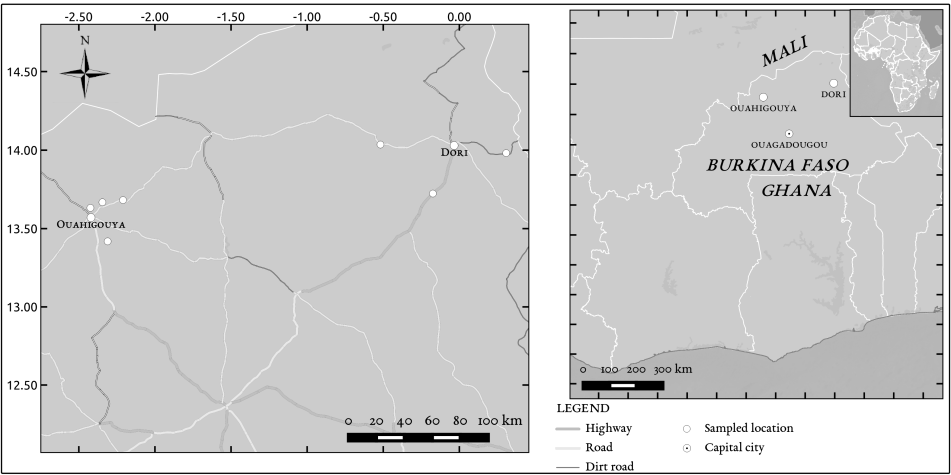
\includegraphics[width=0.9\textwidth]{figs_05/image1.png}
  \captionsetup{singlelinecheck = false, justification=justified}
  \caption{Study areas and sampled villages}
  \label{map:05_1}
  %\small
  %\raggedright
  \vspace*{-3mm}
  \caption*{(Author's composition based on GADM database and Open Steet Maps)}
\end{figure}



Households in both provinces rely largely on rain-fed agriculture. According to the \citet{GlobalYieldGapAtlas2016}, both provinces fall below their potential in terms of crop production. The rain-water limited yield potential in Dori was 2.7 tonnes per hectare for \textit{sorghum} (\textit{bicolor}) and 1.3 tonnes per hectare for millet (predominantly \textit{Pennisetum glaucum L.} possibly also \textit{Eleusine coracana L}), with actual yields estimated to be below one tonne per hectare; water limited yield potential in Yatenga was estimated to be 5.5 tonnes per hectare for sorghum and 2.7 tonnes per hectare for millet, with actual yields also estimated to be below one tonne per hectare.

\subsection{Data}

Fifty households were randomly sampled from four villages in each region, totalling 400 households. Villages were selected based on the following criteria: i) representativeness (e.g. ethnicity, wealth, scale of production), ii) population (at least 500 households), iii) suitability for on-farm trials, and iv) security risk (northern departments/communes in Yatenga were excluded on this basis). Focus group discussions were conducted in the eight villages, each including 20 to 25 participants. Households were then randomly sampled based on full lists of households -- provided by the village leaders. Due to limitations on pre-existing data, sample size was set at 50 households per village -- based on an approximate target of 5 - 10\% of the population (\citealp{Lapan2011}; village household population is presented in Table \ref{tab:05_1}). All selected households agreed to participate. The interview questions were developed based on objectives for the project and the research questions of this study. The questionnaire was pre-tested in each village to ensure the questions were appropriately framed.

Data collection took place in May 2016, administered in French and in local languages when preferred (Fulfulde in Seno province and Moore in Yatenga province). Interviews were conducted by trained enumerators at the respondent's homestead. The household head responded to the majority of questions and other household members were engaged on questions related to food security (e.g. the person who prepares the meals). Respondents were asked detailed questions on household demographics, plot utilisation, livestock holdings, crop yields, farm product utilisation, income, diet, food security, poverty level and labour allocation. Households were asked to recall circumstances from both the most food secure period and the least food secure period of the year (the periods of challenged food security are defined by respondent perceptions of scarcity and presented in the results).

\begin{table}[b]
  \captionsetup{singlelinecheck = false, justification=justified} %left justify caption
  \caption{Number of households by department and village}
  \label{tab:05_1}
  \small
\begin{tabularx}{\textwidth}{@{}lllYY@{}}
  %{
%p{\dimexpr 0.11\linewidth-2\tabcolsep}
%p{\dimexpr 0.25\linewidth-2\tabcolsep}
%p{\dimexpr 0.12\linewidth-2\tabcolsep}
%p{\dimexpr 0.28\linewidth-2\tabcolsep}
%p{\dimexpr 0.23\linewidth-2\tabcolsep}}
\toprule
Province & Department / commune & Village & Households in department${\dag}$ & Households in village${\dag}$ \\
\midrule
Seno & Bani & Bani & 12,102 & 1,030 \\
 & Dori & M'Bamga & 21,366 & 655 \\
 & Gorgadji & Gorgadji & 5,554 & 823 \\
 & Seytenga & Seytenga & 6,102 & 851 \\
Yatenga & Ouahigouya & Aorema & 22,091 & 578 \\
 & & Bogoya & & 879 \\
 & Namissiguima & Tougou & 6,754 & 687 \\
 & Oula & Ziga & 5,536 & 610 \\
 \bottomrule
\end{tabularx}
\footnotesize
\raggedright
%\caption*{
${^\dag}$Census 2006%}
\end{table}



The core indicators assessed in this study were based on from standardised methodologies. `household food insecurity access prevalence' (HFIAP) and `household food insecurity access scale' (HFIAS) were calculated based on the nine food access questions from the `Food And Nutrition Technical Assistance' project (FANTA) guidelines (\citealp{Coates2007}), based on generalised recall of conditions in the `flush' and `lean' periods (full results tabulated in Appendix Table \ref{tab:B1}). `Household diet diversity scores' (HDDS) were calculated using a 12 food category scale as detailed in the FANTA guidelines (\citealp{Swindale2006}), based on recall of both periods. The recall period used in this study are an adaptation of existing guidelines, which suggest using 24-hour recall. This adaptation is designed to provide a more consistent metric -- independent of the timing or duration of survey implementation. The `flush' and `lean' periods of the study were relative to the individual household, where a household could be `food secure' but still report on the most lean period in the year. The indicator was also adjusted to enumerate the channel of HDDS categories (own-farm or purchased).

We calculated several variables on the household for the purpose of our analysis. These variables included the number of inhabitants and nutritional adequacy ratios. Adult equivalents were calculated based on energy requirements relative to adult female and males (averaged) between 25 and 50 (2500 kcal based on energy requirements from \citealp{FoodandAgricuturalOrganization2001}; \citealp{ClaroRafael2010}). Energy adequacy ratios were calculated for home consumed crop and livestock products and protein adequacy ratios were calculated for livestock products only -- based on food composition tables specific to west Africa (\citealp{FAO2012}) -- and a coarse measure of daily energy (2500 kcal adult equivalent$^{-1}$ day$^{-1}$) and protein requirements (56 g adult equivalent$^{-1}$ day$^{-1}$).

Variables calculated to characterise the farm and livelihoods of rural households included: farm production diversity, farm practice adoption, livestock holdings, crop yields, market participation, income, cost of production, gendered control of income and wealth. Farm production diversity has been represented several different ways in the literature (e.g. species count in \citealp{Bellon2016} and \citealp{MKaibi2015}, diet diversity aligned categories in \citet{Koppmair2017325} and \citet{Jones2016} and the debate between the approaches found in the dialogue between \citealp{Berti2015} and \citealp{Sibhatu201510657}). In the present study, we included a measure of crop and livestock diversity (count of species) and production diversity scores (count of products in the HDDS categories). A limitation of the production diversity scores is that they do not capture transformed crop and livestock products (e.g. into fats/oils).

Crop and livestock practice adoption was enumerated for each household, including adoption of irrigation, fertilisation, `improved' seeds, exotic breeds and value addition (adoption rates presented in Appendix Tables \ref{tab:B2} and \ref{tab:B3}). Livestock holdings were represented as Tropical Livestock Units (TLUs; conversion factors from \citealp{Njuki2011a}). Yields for sorghum, millet and maize were calculated based on farmer reported harvest volumes and area planted. Crop market participation was represented as the proportion sold of the total calorific value of crops produced; livestock market participation was represented as the proportion sold of total protein produced from livestock products. The profitability of agricultural enterprises was calculated using respondent estimated cost of production (COP) values where possible (live animals and livestock products), otherwise gross income was reported (crops). Gendered control of income was represented as the percentage of total income that females have autonomous control over. The `progress out of poverty index' (PPI) was calculated from 10 country specific questions on ownership of assets, education and household composition (\citealp{Schreiner2011}).

The cost of production for crops was impacted by item non-response. Due to the high instance of missing data (63\% of crops produced missing) it was not possible to impute these data. The result of this is that crop income is reported in this study as gross income, while livestock income is reported as net income. The proportion of crops sold was only enumerated for species that were marketed, as such missing values were instances where the proportion sold was zero.

\subsection{Statistical analysis}

Our analysis was undertaken in a step-wise manner to describe the potential pathways from intervention to improved food security. We assumed that food insecurity of access and diet diversity are determined by on-farm production and by off-farm sourcing through purchase (i.e. excluding hunting and foraging as there is little scope to intervene in these domains). We therefore first assessed the determinants of food security of access status (HFIAP), followed by the determinants of the on-farm and purchased channels of diet diversity. We also assessed to what extent intensification options are practiced by farmers.

Relationships between core indicators and independent variables were modelled using Bayesian regressions, with random effects from village groupings on the intercept. Regressions were weighted based on village populations to correct for over or under representation in some villages -- i.e. the sum of weightings equated to the sample size for each province. Multinomial regressions were used to model HFIAP, with the least desirable food security outcome as the reference category. Household diet diversity scores were modelled using negative binomial regressions to model the overdispersion in the HDDS variable (i.e. variation not equal to the mean; \citealp{McElreath2016}). Differences between groups were also modelled using a specification equivalent to a t-test, but without assumptions of normality (\citealp{Kruschke2013}).

Models were built in an additive fashion, assessing all potential variables that could influence food security or diet diversity. Priors for the beta coefficients were informed by field knowledge of the interaction of farm and household variables with food security. These prior distributions were informative to the extent that the explanatory variables were expected to be positively associated with food security; these priors were weakly informative in the sense that the ranges of plausible beta coefficients were not restricted. Student's t-distributions were used to this effect, with the mass of the prior distribution being centred to reflect a positive association (centred at 0.5), and the tails thicker than a normal distribution (df = 1) to allow for a greater range of plausible values. If for example, we were to use an exponential prior distribution on beta coefficients for HDDS we would constrain the posteriors to a floor of zero and an unconstrained upper ceiling. This could be reasonable if we are confident that the explanatory variables have a positive relationship with the dependent variable -- however, we have not constrained the models in such a way.

Models were chosen by minimising the Watanabe-Akaike Information Criterion (WAIC). Specifically, this means that if a variable is theorised to influence food security but is not significant in our models, then we only retain it if the WAIC is minimised. Further, convergence was assessed using trace plots, and the model's output Rhat, with chains and iterations adjusted as necessary.

Regressions were implemented in R using the `BRMS' package (v 1.0.1; \citealp{BuerknerP2016}). The `BRMS' package compiles Stan code (http://mc-stan.org/), which uses a hybrid Monte-Carlo Markov Chain (MCMC) method to approximate the posterior distribution of the desired conditional probabilities. Thus the logistic regression models estimate the log odds of an observation being in the higher performing category as opposed to the poorest performing category (severely food insecure) given a unit change in an independent variable, with random effects at the village level; the negative binomial models estimate the log of the expected counts holding all else constant.

\section{Results}

\subsection{Household characteristics and welfare in the two provinces}

There were significant differences in the livelihoods of households between the two provinces. Table \ref{tab:05_2} compares provinces based on variables related to livelihoods that have the potential to influence human nutrition. These variables are presented in the table as follows: resources (adult equivalents, land and livestock ownership), income (including gendered control), wealth (PPI), crop production (diversity, yields, market participation and energy adequacy), and livestock production (diversity, market participation and protein adequacy). There were notable differences between provinces in household demographics, land and land use, market participation, energy/protein adequacy, and income (significant differences indicated in column 4 of Table \ref{tab:05_2}). This section describes the variability and differences in livelihoods.

Household demographics differed across the two provinces. Households in Yatenga province tended to have more inhabitants and therefore, greater potential labour availability and marginally higher nutritional requirements. The household head in Yatenga province was generally older (${\upmu}$ = 57, sd = 12) than in Seno province (${\upmu}$= 50, sd = 13; results not shown), and for the vast majority ({\textgreater} 93\%) of households in both provinces, the household head was male (results not shown).

Households in Yatenga province had larger parcels of land (median of 5 ha) than in Seno province (3.5 ha; Table \ref{tab:05_2}), and the majority of households in both provinces utilised their land for mixed crop-livestock systems. Livestock holdings were similar across provinces, with medians of approximately five Tropical Livestock Units (TLUs); five households in Seno province, however, kept between 25 and 85 TLUs (results not shown). Land was cultivated in the `flush' period with sorghum and millet by almost all farmers; cowpeas (\textit{Vigna unguiculata L.}) were cultivated by the majority of farmers (99\% in Yatenga and 68\% in Seno); sesame (\textit{Sesamum indicum L.}) and maize \textit{(Zea mays L.}) was cultivated by approximately a quarter of farmers; groundnut (\textit{Arachis hypogaea L.}) was cultivated by the majority (96\%) of households in Yatenga province and some households in Seno province (9\%); rice (\textit{Oryza spp.}) production was exclusively in Yatenga province, largely in the Oula department. Vegetable cultivation was also more prevalent in Yatenga, with 20\% of households cultivating up to 1.5 hectares (results not shown). As such, there was greater crop diversity in Yatenga province when compared to Seno province (Table \ref{tab:05_2}).

Yields per hectare of staple crops were lower than the rain-water limited yield potential. Maize was the highest yielding staple crop, followed by the more commonly cultivated staples of sorghum and then millet. Crop yields for these three staple crops were marginally higher in Seno when compared to Yatenga (difference in millet yield was not statistically significant; Table \ref{tab:05_2}). Households differed in their levels of practice adoption. Improved seeds, fertiliser and irrigation were more readily adopted in Yatenga province; and, value addition was common in both provinces. As a proxy for the diversity of cash crop yield differences, Figure \ref{fig:05_1} presents crop income by adopted practices and province. Crop income was significantly higher for households in Yatenga province that adopted irrigation, fertilisers and/or improved seeds (Wilcoxon rank sum test; r = 0.51, 0.20 \& 0.28 respectively; p {\textless} 0.01). In terms of livestock, there was a low level of adoption of improved livestock breeds in both Seno and Yatenga provinces.

\begin{figure}[H]
  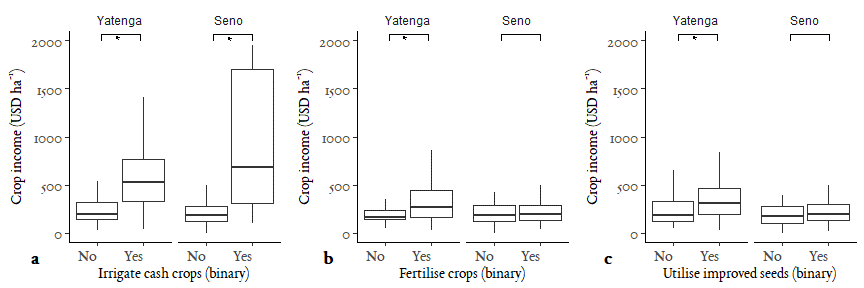
\includegraphics[width=1\textwidth]{figs_05/image2.png}
  \captionsetup{singlelinecheck = off, justification=justified}
  \caption{Gross crop income by practice adoption (irrigation, fertiliser and improved seeds) and province}
  \label{fig:05_1}
  %\small
  %\raggedright
  \vspace*{-3mm}
  \caption*{*Groups have differing central tendencies}
\end{figure}


Larger land sizes and higher rates of market participation in Yatenga province resulted in a higher median energy adequacy ratio and higher median crop income, in comparison to Seno (Table \ref{tab:05_2}). In Yatenga province, households at the median were potentially self-sufficient in energy needs; in Seno province, the median energy adequacy ratio was below sufficiency, with 80\% of energy needs met by home consumption of crops and animal-source foods. Livestock market participation was more common in Seno province, as was consumption of home-produced livestock products -- as shown in the higher adequacy ratio of protein from animal sources and higher median income from livestock products (Table \ref{tab:05_2}).

Off-farm income was common across provinces (67\% of households in Yatenga, 57\% of households in Seno), with the majority earning under US\$500 per household per annum. For those that did earn off-farm income, the central tendency of earnings was similar across provinces (median of US\$296 in Yatenga and US\$375 in Seno). Households in Yatenga generally had higher gross incomes, yet significantly less income from live animals (Table \ref{tab:05_2}). Control of income did not differ significantly by province, where the majority (85\%) of households had less than 10\% of income controlled by females. Households in Yatenga province tended to have a higher Progress out of Poverty Indicator score (PPI).



\begin{table}[H]
  \captionsetup{singlelinecheck = false, justification=justified} %left justify caption
  \caption{Summary of resources and farming activity of households (median and IQR)}
  \label{tab:05_2}
  \small
\begin{tabularx}{\textwidth}
  {
  p{\dimexpr 0.45\linewidth-2\tabcolsep}
  YYY}
%p{\dimexpr 0.23\linewidth-2\tabcolsep}
%p{\dimexpr 0.23\linewidth-2\tabcolsep}
%p{\dimexpr 0.09\linewidth-2\tabcolsep}}
\toprule
Characteristic & Yatenga & Seno & \\
 & (n = 200) & (n = 200) & \\
 \midrule
Household inhabitants (adult eq.) & 10.4 (5.4) & 6.8 (5.3) & * \\
Land area (ha) & 5.0 (4.1) & 3.5 (3.0) & * \\
Livestock holdings (TLUs)$^{\mathrm{a}}$ & 5.20 (4.8) & 5.1 (9.0) & NS \\
\arrayrulecolor{black!30}\midrule
Off-farm income (USD year$^{-1}$)$^{\mathrm{b}}$ & 83.25 (451.62) & 74.92 (416.24) & NS \\
Crop gross income (USD year$^{-1}$)$^{\mathrm{b}}$ & 354.56 (637.55) & 0.00 (8.11) & * \\
Live animal net income (USD year$^{-1}$)$^{\mathrm{b}}$ & 12.49 (97.90) & 60.84 (248.72) & * \\
Animal product net income (USD year$^{-1}$)$^{\mathrm{b}}$ & 0 (0) & 0 (0) & NS \\
Relative female control (\% income year$^{-1}$) & 0 (2) & 0 (0) & * \\
Progress out of Poverty Index score & 38 (14) & 31 (16) & * \\
\arrayrulecolor{black!30}\midrule
Number of crop species & 5 (2) & 3 (2) & * \\
Crop production diversity & 2 (1) & 2 (0) & * \\
Sorghum yield (kg ha$^{-1}$) & 225.0 (338.0) & 250.0 (250.0) & * \\
Millet yield (kg ha$^{-1}$) & 184.0 (350.0) & 217.0 (350.0) & NS \\
Maize yield (kg ha$^{-1}$) & 650 (985.0) & 720.0 (725.0) & * \\
Crop market participation (\% of total calories produced year$^{-1}$) & 41 (26) & 0 (1) & * \\
Crops consumed (kcal adequacy ratio adult equivalent$^{-1}$) & 1.00 (1.1) & 0.8 (0.7) & * \\
\arrayrulecolor{black!30}\midrule
Number of livestock species & 4 (2) & 4 (2) & NS \\
Livestock production diversity score & 1 (0) & 2 (1) & NS \\
Livestock market participation (\% of protein produced year$^{-1}$) & 0 (0) & 0 (3) & NS \\
Livestock products consumed (protein adult equivalent$^{-1}$ adequacy ratio) & 0.02 (0.02) & 0.15 (0.27) & * \\
\arrayrulecolor{black}\bottomrule
\end{tabularx}
\footnotesize
\raggedright
%\caption*{
*CI does not cross zero. Provinces have differing central tendencies\\
$^NS$CI crosses zero or model does not converge\\
$^a$Oxen = 1.42, cows = 1, camel = 1.1, horse = 0.9, donkey = 0.8, pigs = 0.3, sheep and goats = 0.2, chickens = 0.04\\
$^b$1 CFA = 0.001665 USD%}
\end{table}



\subsection{Determinants of food (in)security of access}

Households had differing perceptions of the severity and duration of food insecurity. In Yatenga province, the most common period of perceived shortage was between February and October (27\% of households). In Seno province 43\% of households perceived a shortage of food between June and October. Many households perceived that they had just enough food throughout the year (27\% in Yatenga and 20\% in Seno), and a few households considered themselves to be food secure throughout the year (8\% in Yatenga and 6.5\% in Seno). There was only one household per province that perceived a shortage in the period between November and February, where the majority of households considered themselves to be secure during this time. For the following analysis, the `flush' period can be considered as this period between November and February and the `lean' period as being more variable in duration and severity -- between February and October. Aid in the form of food or money was distributed in the study area. In Yatenga province, 40\% of households received aid, whereas in Seno province, only two households received aid. The most common period of aid provision was between June and October (results not shown).

The majority of households in the `lean' period were classified as either `severely food insecure' or `moderately food insecure' using the Household Food Insecurity Access Prevalence (HFIAP) indicator. In Yatenga province, approximately 31\% of households were classified as `severely food insecure' in the `lean' period, 41\% as `moderately food insecure', 17\% as `mildly food insecure' and 10\% as `food secure'. The food security status of households in Seno province was worse, with over 84\% of households classified as being `severely food insecure' in the `lean' period, 13\% classified as `moderately food insecure', 2\% classified as `mildly food insecure' and less than 2\% classified as `food secure'.

The HFIAS variable was modelled as a function of gross income (off-farm, crop and livestock), gendered control of income, energy adequacy, species diversity, whether aid was received and province of residence. There was a positive association between gross income and a higher food security of access status (i.e. not severely food insecure) in both provinces in the `lean' period; this association was stronger in Yatenga -- indicated by the significant interaction term (Table \ref{tab:05_3}). The number of livestock species kept was positively associated with a higher food security of access status in the `lean' period. Consumption adequacy, the number of crop species and receiving aid were not associated with food security of access in the `lean' period (Table \ref{tab:05_3}). Furthermore, there were no statistically significant associations identified for relative female control, higher food security status or the number of crop species cultivated in the `flush' period.



\begin{table}[H]
  \captionsetup{singlelinecheck = false, justification=justified} %left justify caption
  \caption{Household Food Insecurity Access (logistic regressions${\dag}$)}
  \label{tab:05_3}
  \small
\begin{tabularx}{\textwidth}%{@{}lYY@{}}
  {
p{\dimexpr 0.48\linewidth-2\tabcolsep}
Y Y}
%p{\dimexpr 0.26\linewidth-2\tabcolsep}
%p{\dimexpr 0.27\linewidth-2\tabcolsep}}
\toprule
Fixed effects & Lean period$^{\mathrm{a}}$ & Flush period$^{\mathrm{a}}$ \\
 \midrule
Intercept & -2.44 (-5.20, 0.04) & 1.08 (-1.76, 4.59) \\
Gross income (`000 USD year$^{-1}$) & 0.34 (0.08, 0.64) * & 0.16 (0.02, 0.36) * \\
Food consumed from own farm (kcal adequacy ratio adult equivalent$^{-1}$) & -0.18 (-0.45, 0.01) & 0.02 (-0.09, 0.15) \\
Number of crop species & 0.11 (-0.16, 0.37) & 0.09 (-0.18, 0.34) \\
Number of livestock species & 0.32 (0.10, 0.55) * & 0.08 (-0.12, 0.28) \\
Aid received$^{\mathrm{b}}$ & 0.08 (-0.82, 0.97) & 0.13 (-0.93, 1.17) \\
Province$^{\mathrm{c}}$ & -0.62 (-2.22, 1.11) & -0.63 (-2.30, 1.20) \\
\arrayrulecolor{black!30}\midrule
Gross income:province & -0.53 (-0.95, -0.17) * & \\
\arrayrulecolor{black}\bottomrule
\end{tabularx}
\footnotesize
\raggedright
%\caption*{
$^{\dag}$ Estimates are presented as posterior ${\upbeta}$ estimate and 95\% credible interval (CI)\\
* CI does not cross zero\\
$^a$Reference category is `severely food insecure of access'\\
$^b$Reference category for dichotomous variable is `no'\\
$^c$Reference category is Yatenga province\\%}
\end{table}



\subsection{Determinants of household diet diversity}

The household diet diversity score differed across periods and provinces. In general, diets were more diverse in the `flush' period and households in Yatenga province tended to have more diverse diets in the `lean' period than households in Seno province (intercepts and province coefficient in Table \ref{tab:05_4} and medians in Table \ref{tab:05_5}). Table \ref{tab:05_4} presents regression outputs for HDDS in both the `lean' and `flush' periods. In the `lean' period there are interactions between gross farm income, off-farm income and province, which makes the associations difficult to interpret from the combination of coefficients; these interactions are best visualised as marginal effects. Figure \ref{fig:05_2} presents the associations between gross farm income and diet diversity in the `lean' period. Gross farm income was positively associated with diet diversity in Yatenga province in the `lean' period, particularly for households that did not earn off-farm income. In Seno province these associations differ, where diet diversity in the `lean' period is predicted to increase as gross farm income increases -- only when off-farm income is also earned. Households that did not earn off-farm income in Seno province were predicted to decreased in diet diversity in the `lean' period as gross farm income increased.

Crop species diversity was also positively associated with diet diversity in the `lean' period -- regardless of province. This statistically significant association, however, did not persist when assessing crop production diversity (count of crop products in HDDS categories) -- which, by definition, has a closer association with HDDS.

We also assessed whether: a) the influence of farm income on diet diversity is mediated by female control, and b) food self-sufficiency is positively associated with diet diversity. However, female control of income and food self-sufficiency were not found to be associated with diet diversity in this study.



\begin{table}[H]
  \captionsetup{singlelinecheck = false, justification=justified} %left justify caption
  \caption{Household diet diversity (Mixed-effects negative binomial regressions${\dag}$)}
  \label{tab:05_4}
  \small
\begin{tabularx}{\textwidth}{@{}lYY@{}}
%  {
%p{\dimexpr 0.55\linewidth-2\tabcolsep}
%p{\dimexpr 0.24\linewidth-2\tabcolsep}
%p{\dimexpr 0.21\linewidth-2\tabcolsep}}
\toprule
 Fixed effects & Lean period & Flush period \\
 \midrule
Intercept & 1.26 (1.03, 1.50) * & 2.00 (1.78, 2.21) * \\
Gross farm income (`000 USD year$^{-1}$) & 0.01 (-0.06, 0.07) & 0.02 (-0.01, 0.04) \\
Off-farm income earned$^{\mathrm{a}}$ & 0.13 (0.01, 0.26) * & 0.05 (-0.03, 0.14) \\
Relative female control ({\textgreater} 40\% income year$^{-1}$) & 0.08 (-0.07, 0.22) & -0.04 (-0.16, 0.09) \\
Number of crop species & 0.05 (0.01, 0.09) * & 0.01 (-0.02, 0.04) \\
Number of livestock species & 0.00 (-0.03, 0.04) & 0.01 (-0.01, 0.04) \\
Province$^{\mathrm{b}}$ & -0.31 (-0.52, -0.09) * & -0.02 (-0.26, 0.22) \\
\arrayrulecolor{black!30}\midrule
Gross farm income:off-farm income earned & 0.03 (-0.05, 0.12) & \\
Gross farm income:province & -0.10 (-0.19, 0.00) * & \\
Off-farm income earned:province & 0.08 (-0.10, 0.25) & \\
Gross farm income:off-farm income earned:province & 0.16 (0.04, 0.28) * & \\
\arrayrulecolor{black}\bottomrule
\end{tabularx}
\footnotesize
\raggedright
%\caption*{
$^{\dag}$Estimates are presented as posterior ${\upbeta}$ estimate and 95\% credible interval (CI)\\
*CI does not cross zero\\
$^a$Reference category for dichotomous variable is `no'\\
$^b$Reference category is Yatenga province\\%}
\end{table}





\begin{figure}[H]
  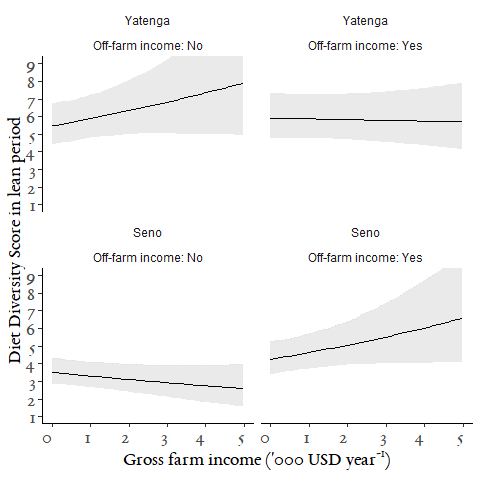
\includegraphics[width=0.5\textwidth]{figs_05/image3.png}
  \captionsetup{singlelinecheck = off, justification=justified}
    \caption{Household diet diversity dcore in the `lean' period. Marginal effects of gross income (`000 USD) by off-farm income and province; dashed lines indicate uncertainty of marginal effect estimates at a 95\% credible interval. All associations represented are statistically significant}
    \label{fig:05_2}
\end{figure}

The channel of access of food categories provides a disaggregated view of HDDS. In both provinces and periods, purchased diversity was a greater point of differentiation than farm-sourced diversity (Table \ref{tab:05_5}). The median number of purchased food categories was three times as much as own farm-sourced categories in the `lean' period and more than double own farm-sourced categories in the `flush' period. Farm-sourced categories were largely limited to the cereals and `pulses, legumes and nuts' categories, with some households having the addition of vegetables, eggs, meat and/or milk (results not shown).


\begin{table}
  \captionsetup{singlelinecheck = false, justification=justified}
  \caption{Summary of Household diet diversity score for households (HDDS; median and IQR)}
  \label{tab:05_5}
  \small
\begin{tabular}{L{7.3cm} C{3cm} C{3cm} C{1cm}} %Page is 14.3cm across %{\textwidth}{@{}lYYY@{}}
  %{
%p{\dimexpr 0.44\linewidth-2\tabcolsep}
%p{\dimexpr 0.2\linewidth-2\tabcolsep}
%p{\dimexpr 0.21\linewidth-2\tabcolsep}
%p{\dimexpr 0.15\linewidth-2\tabcolsep}}
\toprule
 & Seno (n = 200) & Yatenga (n = 200) &  \\
 \midrule
HDDS - lean period & 3.5 (3.0) & 6.0 (2.0) & * \\
HDDS - flush period & 8.0 (4.0) & 9.0 (1.0) & \\
HDDS from farm production - lean period & 1.0 (1.0) & 2.0 (2.0) & * \\
HDDS purchased - lean period$^{\mathrm{a}}$ & 3.0 (3.0) & 6.0 (2.0) & * \\
HDDS from farm production - flush period & 3.0 (2.0) & 3.0 (2.0) & * \\
HDDS purchased -- flush period & 7.0 (5.0) & 7.0 (2.0) & \\
\bottomrule
\end{tabular}
\footnotesize
\raggedright
%\caption*{
*Provinces have differing central tendencies\\
$^a$Observations with no purchased food in the `lean' period removed (n = 8 from Yatenga province)%}
\end{table}



At the aggregate level, the own-farm channel of food access had a limited association with diet diversity. This is understandable, where in the `lean' period, households in tended to source only one or two food categories from their farm (Table \ref{tab:05_5}). At the disaggregated level, the number of crop species cultivated is associated with diet diversity accessed through the own-farm channel in the `lean' period (Table \ref{tab:05_6}). In the `flush' period, both the number of crop and livestock species are associated with diet diversity accessed through the own-farm channel. These associations persisted when assessing crop and livestock production diversity instead of species diversity (results not shown).


\begin{table}
  \captionsetup{singlelinecheck = false, justification=justified}
  \caption{Household diet diversity accessed through own-farm channel (mixed-effects negative binomial regression${\dag}$)}
  \label{tab:05_6}
  \small
\begin{tabularx}{\textwidth}{@{}lYY@{}}
  %{
%p{\dimexpr 0.42\linewidth-2\tabcolsep}
%p{\dimexpr 0.29\linewidth-2\tabcolsep}
%p{\dimexpr 0.29\linewidth-2\tabcolsep}}
\toprule
Fixed effects & Lean period & Flush period \\
 \midrule
Intercept & -0.08 (-0.69, 0.52) & 0.75 (0.38, 1.13) * \\
Number of crop species & 0.11 (0.05, 0.18) * & 0.05 (0.00, 0.10) * \\
Number of livestock species & 0.03 (-0.03, 0.08) & 0.05 (0.01, 0.09) * \\
Province$^{\mathrm{a}}$ & 0.24 (-0.54, 1.04) & 0.26 (-0.18, 0.73) \\
\bottomrule
\end{tabularx}
\footnotesize
\raggedright
%\caption*{
$^{\dag}$Estimates are presented as posterior ${\upbeta}$ estimate and 95\% credible interval (CI)\\
*CI does not cross zero\\
$^a$Reference category is Yatenga province.%}
\end{table}



At the disaggregated level, there is greater uncertainty around the interactions between purchased diet diversity, farm income, off-farm income and province (Table \ref{tab:05_7}). At this disaggregated level we also see an association between the number of crop species cultivated and purchased diet diversity in the `lean' period. This association cannot be considered causal as the own-farm channel of food access is not represented in Table \ref{tab:05_7}. Rather, this result informs us that the purchased channel to diet diversity is not impeded by crop species diversity.

\begin{table}[H]
  \captionsetup{singlelinecheck = false, justification=justified}
  \caption{Household diet diversity accessed through purchased channel (mixed-effects negative binomial regression${\dag}$)}
  \label{tab:05_7}
  \small
\begin{tabularx}{\textwidth}{@{}lYY@{}}
  %{
%p{\dimexpr 0.55\linewidth-2\tabcolsep}
%p{\dimexpr 0.24\linewidth-2\tabcolsep}
%p{\dimexpr 0.21\linewidth-2\tabcolsep}}
\toprule
 Fixed effects & Lean period$^{\mathrm{a}}$ & Flush period \\
 \midrule
Intercept & 1.23 (1.01, 1.46) * & 1.81 (1.51, 2.12) * \\
Gross farm income (`000 USD year$^{-1}$) & 0.04 (-0.02, 0.09) & 0.00 (0.00, 0.00) \\
Off-farm income earned$^{\mathrm{b}}$ & 0.14 (0.01, 0.27) * & 0.05 (-0.05, 0.15) \\
Relative female control ({\textgreater} 40\% calories year$^{-1}$) & 0.07 (-0.09, 0.23) & -0.07 (-0.21, 0.06) \\
Number of crop species & 0.04 (0.00, 0.09) * & 0.02 (-0.02, 0.05) \\
Number of livestock species & -0.01 (-0.05, 0.02) & 0.01 (-0.02, 0.04) \\
Province$^{\mathrm{c}}$ & -0.35 (-0.52, -0.16) * & 0.00 (-0.37, 0.39) \\
\arrayrulecolor{black!30}\midrule
Gross farm income:off-farm income earned & -0.00 (-0.08, 0.07) & \\
Gross farm income:province & -0.05 (-0.12, 0.03) & \\
Off-farm income earned:province & 0.14 (-0.05, 0.33) & \\
Gross farm income:off-farm income earned:province & 0.09 (-0.02, 0.20) & \\
\arrayrulecolor{black}\bottomrule
\end{tabularx}
\footnotesize
\raggedright
%\caption*{
$^{\dag}$Estimates are presented as posterior ${\upbeta}$ estimate and 95\% credible interval (CI)\\
*CI does not cross zero\\
$^a$Observations with no purchased food in the `lean' period removed (n = 8 from Yatenga province)\\
$^b$Reference category for dichotomous variable is `no'\\
$^c$Reference category is Yatenga province.\\%}
\end{table}



\section{Discussion}

Our analysis shows that in both provinces, the ability to purchase food is what differentiates the more food secure households from their less food secure counterparts. This finding does not detract from the utility of subsistence production -- where consumption of own-farm food tended to cater for 91\% of the annual energy requirements in Yatenga province and 72\% in Seno province. Rather, purchasing power was the differentiating factor between households with food availability and those that are more food secure. This differentiation of households is most apparent in the dietary diversity indicator, where in both `flush' and `lean' periods, purchased food groups are more numerous than consumption of own-farm produced food groups (Table \ref{tab:05_5}). This is logical in this setting where at maximum, households could source nine of the twelve categories from their farm (including processing oil); realistically, households were observed to source two to three categories from their farm in the `flush' period (similar findings in \citealp{Some2018}). These farm-sourced categories were largely limited to the cereals and `pulses, legumes and nuts' categories. This finding is consistent with the majority of recent studies on the relative importance of purchased/farm-sourced foods (\citealp{Bellon2016}; \citealp{Koppmair2017325}; \citealp{Luckett20152479}; \citealp{Sibhatu201510657}; \citealp{Snapp2015}; and \citealp{Dillon2014}). Similarly, \citet{Jones2016}, while emphasising the importance of diverse farm production across wealth strata, noted that the relationship between production diversity and diet diversity may be mediated through income generation (and thus purchased food), as well as farm-sourced food groups. With a growing consensus, can it then be concluded (as implicit in the aims of \citealp{FAO2016a}) that food insecurity will be eradicated by doubling the `agricultural productivity and incomes of small-scale producers' through on-farm means and off-farm employment/business? Food security is not simply limited to an individual's capacity to access calories. Other important dimensions of food security include: protein and micro-nutrient intake, resilient agricultural practices, maintaining genetic diversity of plants and animals, and maintaining access to culturally relevant foods (\citealp{FAO2008}). Further, the allocation of scarce household resources is not solely dedicated to achieving food security. Households use their income to pursue multiple goals (e.g. education), and the allocation of resources depends on needs (including food security and other higher order needs) and complex intra-household dynamics (\citealp{Kazianga2017}; \citealp{Galie2015}).

\subsection{Towards a pathway model of food security}

The potential pathways from food and income availability to food security analysed in this study are represented diagrammatically in Figure \ref{fig:05_3}. The diagram includes farm resources and activities from Table \ref{tab:05_1} and Figure \ref{fig:05_1} on the left-hand-side, representing the basis for food production. Both market and subsistence (own-farm) channels to food security are represented in a flow (indicated by arrows) from the left-hand-side towards the right-hand-side. Market participation, off-farm income and aid all contribute to net income. Mediated through expenditure and consumption decisions, these two channels of food access (purchased and own-farm) then have a bearing on the availability of food, energy access, diversity of food access, access to culturally relevant foods, and stability of food security over time (right-hand-side of Figure \ref{fig:05_3}). The pathways from food and income availability to food security may also influence the pattern of food utilisation within a household. This dimension of food security, however, is beyond the scope of this study.

\begin{figure}[H]
  \captionsetup{singlelinecheck = false, justification=justified}
  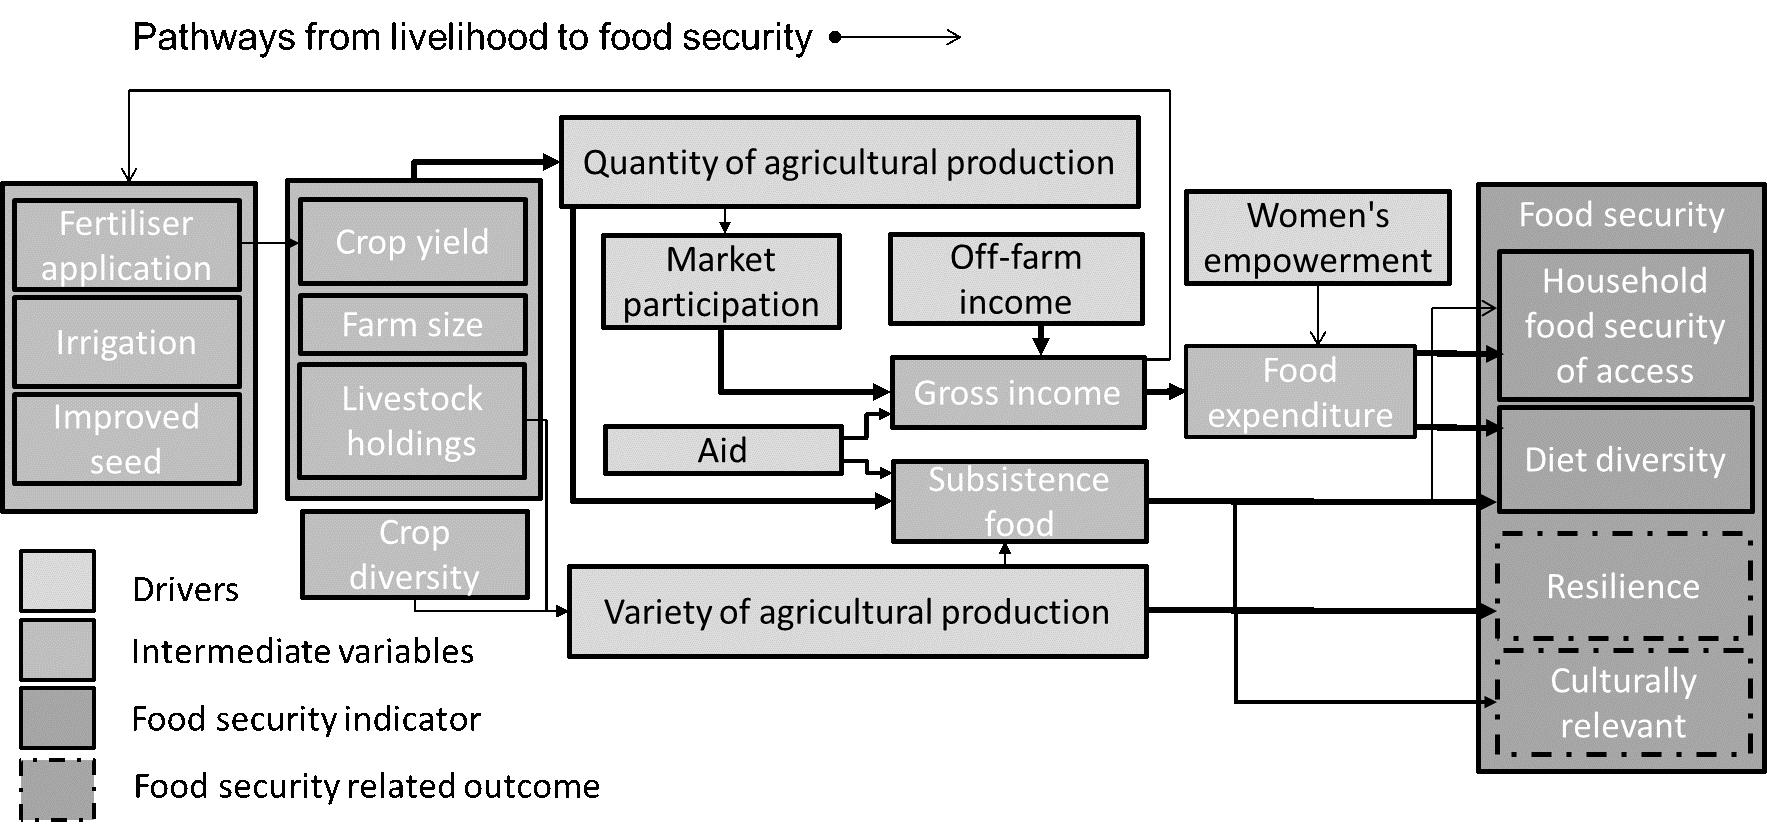
\includegraphics[width=1\textwidth]{figs_05/image4.png}
  \caption{Pathways to food security outcomes (adapted from \citealp{Jones2016})}
  \label{fig:05_3}
\end{figure}

The relationship between crop diversity and the diversity of food access is a central area of inquiry in the literature. Previous studies have used this relationship to draw conclusions on whether to reduce hidden hunger by supporting market-oriented interventions (upper drivers in Figure \ref{fig:05_3}) or by promoting agrobiodiversity (lower driver in Figure \ref{fig:05_3}). Our results suggest that these goals do not have to be mutually exclusive. Both gross income and livestock species diversity, for example, are associated with improved food security of access. Similarly, both gross farm income and crop species diversity were associated with more diverse diets. Considering the implications of this more generally, livestock keeping -- as part of a diversified portfolio -- provides soil health benefits through the recycling of nutrients, as well as reducing livelihood risk by acting as a means to store capital (\citealp{Moll2005}; \citealp{Slingerland2000}). Similarly, diversified crop production can contribute to pest and disease management; reduce the market risk of volatile prices, and; can also be a part of a soil health strategy (e.g. nitrogen fixation or cover cropping to reduce erosion; \citealp{Lin2011}). Each of these benefits can improve the resilience of a farm and a livelihood (contributing to stability in Figure \ref{fig:05_3}), specifically in relation to climatic or economic shocks.

The majority of households cultivated sorghum and millet. Access to such culturally relevant and nutritious foods is not guaranteed in the future (\citealp{Schipanski2016}; \citealp{Pingali2015}; \citealp{Remans2014}). The global trend of increasing food homogeneity (e.g. \citealp{Khoury2014}) has already resulted in traditional, lower yielding grains such as tef (Eragrostis tef), millet (\textit{Pennisetum glaucum L}. and \textit{Eleusine coracana L}) and sorghum (Bicolour) being substituted with maize (\textit{Zea mays L.}), traditional vegetables replaced with market vegetables, and narrowed livestock genetic resources. The potential trade-offs between energy availability, resilience and the availability of culturally relevant and nutritious foods need to be considered to be able to optimise all aspects of food security. These trade-offs could be addressed -- in part -- by increased investment in locally relevant breeding (\citealp{Sibhatu201510657}) and the coupling of soil health education with fertiliser-based intensification programs (\citealp{Fonte2012}). Plant breeding can work to optimise yields and micro-nutrient bioavailability (increasing translocation and reducing inhibition) of locally relevant crops; and soil health can maintain/increase yields and improve soil micro-nutrient availability for the plants and ultimately the household (\citealp{DeValenca2017}; \citealp{Slingerland2006}).

The `income pathway' to improved food security has not been fully captured in all its complexity in this study. We observed significant differences in median crop income based on practice adoption. This relationship may be bi-directional, with higher incomes allowing practice adoption (represented as an arrow from gross income to practices on the left-hand-side of Figure \ref{fig:05_1}), and practice adoption increasing crop incomes. We also observed associations between gross income and food security (food security of access and diet diversity; Tables \ref{tab:05_3} and \ref{tab:05_4}). These associations differed substantially by province and whether off-farm income was earned (in the case of diet diversity). In this study, however, we did not identify any associations or interactions between female control of income and food security -- which by no means negates the reality that intra-household dynamics influence food access or food utilisation (e.g. \citealp{Mason2015}).

Off-farm income was more common in Yatenga (67\% of households in Yatenga compared to 57\% in Seno), but proved to be a greater differentiating factor in Seno. Having a wage or business income is an apparent advantage over a reliance on agriculture (\citealp{Reardon1992}). In Seno this advantage provides a pathway to a greater variety of food categories in the `lean' period -- when households are at their most vulnerable. From a policy and intervention perspective, there are macro-economic factors, regional comparative advantages and a range of other elements that drive the opportunities to engage in employment or business. With a growing rural population there is a need to improve rural non-farm opportunities (e.g. \citealp{Jayne2014}; \citealp{Haggblade2010}; \citealp{Tiffen2003}). This finding suggests that interventions to stimulate such opportunities can be targeted at specific regions or communities to improve household food security. A challenge that may arise in the process of stimulating off-farm opportunities, however, is that the individuals that capture them may not be the most in need; evidence suggests that wealthier households have a greater capacity to gain employment or invest in a non-farm business (\citealp{Davis2010}; \citealp{Haggblade2010}; \citealp{Reardon1992}). The complexities of the labour market are such that not only do the opportunities have to exist, but there also needs to be the availability of quality education options (\citealp{Jayne2014}) and functioning land tenure, credit and insurance markets (\citealp{Barrett2001}).

Aid (a potential driver of improved food security in Figure \ref{fig:05_3}) was received by a small portion of households in Yatenga province. There was no significant difference in food security status between recipients of aid and other respondents. This is not enough, however, to conclude whether this aid was effective in improving the food security of these households.

The experimental design of this study allowed us to improve our understanding of the causal pathways to improved food security in two subtly contrasting communities in drought prone regions of Burkina Faso. There are, however, some methodological limitations to our approach. Firstly, the sampling of this study was limited to eight villages within seven departments with some departments of Yatenga province excluded from sampling due to safety concerns. Conflict has been identified as an important driver of food insecurity (\citealp{FAO2018}) and so the results of this study cannot be taken to be representative of northern Yatenga. The limitation in sampling, however, necessitated the use of 1) weightings to correct the representativeness of our study and 2) a power analysis to assess the risk of Type II errors. A post-hoc analysis indicated that at a power of 0.8 (20\% risk of Type II error), these data allowed the detection of small differences in central tendency (Cohen's d {\textless} 0.2; results not tabulated elsewhere). Secondly, we enumerated food security indicators and farm production/marketing based on respondent recall. The complexity and length of recall may have negatively impacted measurement precision and item non-response (\citealp{Beegle2012}). To counteract this, we designed the survey to minimise respondent fatigue and we trained enumerators to cross-check responses to more complex questions. These design features, unfortunately, did not enable us to enumerate the cost of crop production -- which suffered from item non-response. Thirdly, as identified by \citet{Some2018}, we interviewed the household head on-farm activities -- potentially underestimating production diversity.

The food security status of households is most substantially and positively influenced by a household's ability to purchase food. This finding should not detract from the essential role played by subsistence production. Rather, market-orientated agriculture and production for home consumption, as shown by households in this study, can be combined as part of a broader livelihood strategy. Such livelihood strategies can improve food access and the stability of food security in both the `flush' and `lean' periods.

\section{Acknowledgments}

We thank the field team for their dedication and the participating rural households for their candor. This study was made possible by the support of the American People provided to the Feed the Future Innovation Lab for Sustainable Intensification through the United States Agency for International Development (USAID). The contents are the sole responsibility of the authors and do not necessarily reflect the views of USAID or the United States Government. Program activities are funded by the United States Agency for International Development (USAID) under Cooperative Agreement No. AID-OAA-L-14-00006. Also support by the CGIAR Research Program on Livestock is gratefully acknowledged.

\chapter[Dietary gaps in sub-Saharan Africa: prevalence and implications for agricultural interventions]{Dietary gaps in sub-Saharan Africa: prevalence and implications for agricultural interventions}
\chaptermark{Dietary gaps in sub-Saharan Africa}
\label{cha:chapter6}
\vspace*{\fill}
This chapter is based on:
\\
\\
% Full citation of the published (or submitted/in review) article
% This refers to the article key in the refs.bib file.
Fraval, S., Hammond, J., Bogard, J. R., Ng'endo, M., van Etten, J., Herrero, M., Oosting, S. J., de Boer, I. J. M., Lannerstad, M., Teufel, N., Lamanna, C., Rosenstock, T. S., Pagella, T., Vanlauwe, B., Dontsop-Nguezet, P. M., Baines, D., Carpena, P., Njingulula, P., Okafor, C., Wichern, J., Ayantunde, A., Bosire, C., Chesterman, S., Kihoro, E., Rao, J., Skirrow, T., Steinke, J., Stirling, C. M., Yameogo, V., van Wijk, M. T. (submitted). \textit{Global Food Security}

\newpage

\section*{Abstract}
Efforts to estimate the prevalence of food insecurity and to understand its associations with rural livelihoods has been hampered by limitations in temporal and spatial representativeness. Food balance sheets provide scalable estimates of chronic and hidden hunger, but fail to represent food access, stability and their causal linkages. In contrast, rural household surveys represent detailed conditions for one or two points of time, but are influenced by survey timing and are often limited in geographical coverage. This study draws on a large sample of rural land-holding households in SSA (n = 6,353; 54\% of which were from semi-arid zones) to estimate the prevalence of dietary gaps and to understand their associations with rural livelihoods and food sourcing behaviour throughout the year. Dietary gaps were identified using diet diversity and food access indicators. Dietary diversity and channel of access (farm or purchased) were enumerated for the `flush' and `lean' periods and food security of access was enumerated for the lean period only -- making the results of this study independent of survey timing. The identified dietary gaps were then compared with quantified dietary adequacy ratios of subsistence households, and only included in further analysis if there was a statistically significant association. As many as 40\% of households were classified as severely food insecure (in terms of food access) in the lean period. Prevalence of micronutrient dietary gaps were high, with 68\% lacking daily calcium sources, 38\% lacking daily sources of iron, 37\% lacking daily sources of thiamine, 51\% lacking daily sources of riboflavin, 44\% lacking daily sources of niacin, 35\% lacked a source of vitamin B6 and 65\% lacking daily sources of vitamin B12. Vulnerability to dietary gaps differed by household composition and agricultural livelihood characteristics. Market participation, livestock product diversity, crop production diversity, gross income and off-farm income were all positively associated with food security of access and micronutrient access. These associations differed between agro-ecological zones and were predicted to have a limited impact on dietary gaps. Households with a livestock component to their farm consumed more milk, meat and eggs (sources of calcium, riboflavin and vitamin B12). Dairy, fruit and vitamin A-rich produce were  predominantly accessed through the farm channel. Households with a livestock component to their farm had a lower prevalence of severe food insecurity and gaps in micronutrient sources.

These findings have implications for the development of nutrition-sensitive and nutrition-specific interventions. Interventions need to be tailored to agroecological zone, household composition, scale of operation and production mix. Increasing income will not necessarily result in improved diet diversity or healthy dietary choices. Interventions focused on income generation should monitor and promote crop and livestock production diversity and provide nutrition education. Our analysis suggests that it is unrealistic or may even be counterproductive to try and shift overall diet diversity substantially, rather it is more useful to target individual food groups that will benefit human nutrition.

\newpage

\section{Introduction}

Almost one in four people in sub-Saharan Africa (SSA) were estimated to be undernourished in 2017, representing about one-third of the 821 million people suffering from chronic hunger globally (\citealp{FAO2018}). In addition to a high prevalence of chronic hunger in SSA, many more people suffer from micronutrient deficiencies (\citealp{Harika2017, Kumssa2015, Joy2014}). These deficiencies increasingly co-exist with instances of obesity within the same communities -- forming a triple burden on human health and society (\citealp{May2018}). Malnutrition is now the greatest risk factor driving a rising global noncommunicable  disease burden (\citealp{GBD2016RiskFactorsCollaborators2017}), having direct implications for child growth failure, neonatal disorders, immune function, cognitive function, diabetes, heart disease and cancer (\citealp{James2018}; \citealp{Prentice2018}; \citealp{DePee2017}; \citealp{Pisa2017}; \citealp{Akombi2017}; \citealp{Micha2015}). These burdens will only intensify as rural and urban populations grow, diets change and wealth is further concentrated (\citealp{FAO2018}; \citealp{Popkin2014}).

The majority of the food in SSA is produced by smallholder farmers (\citealp{Herrero2017}) while they are the most vulnerable to food insecurity and poverty (\citealp{Fanzo2018}; \citealp{Sibhatu2017}). Hence, smallholder farmers are a crucial entry point for agricultural orientated interventions to improve food and nutrition security. A substantial number of observational studies have assessed the linkages between agriculture and nutrition in the past three years (e.g. \citealp{Ruel2018}; \citealp{Gillespie2017}). Despite progress in the analysis of existing observational data and ex-post evaluation of nutrition-sensitive interventions, much remains to be understood with respect to the pathways of intervention to improved food and nutrition security of rural households (\citealp{Mary2018}).

The causal pathways from intervention to food and nutrition security outcomes are not straightforward (\citealp{Carletto2017}). An important question, not yet answered by the existing literature (e.g. \citealp{Ruel2018}; \citealp{Gillespie2017}) relates to how market participation mediates food and nutrition security in rural communities -- especially access to and consumption of diverse diets. Farmers have two ways to obtain their food: 1) growing food crops and/or rearing livestock to consume the products, or 2) selling these products and use the income to buy food for their own consumption. Whether production-based or income-based channels are more important for food and nutrition security is a question without a straightforward answer. For example, increased incomes and energy availability are necessary for alleviating undernourishment but are not sufficient for addressing chronic or hidden hunger (\citealp{Godecke2018}; \citealp{Schipanski2016}; \citealp{McDermott2015}; \citealp{Hoddinott2012}). These causal pathways need to be considered in targeting, designing and implementing nutrition-sensitive interventions of agricultural production systems and value-chains.

Evaluating food access and micro-nutrient deficiencies has traditionally been time-consuming and invasive. More recently, however, proxies have been introduced to enable wide-scale monitoring and evaluation. Food security of access scales and diet diversity scores (to a greater extent) have been favourably assessed as proxies for nutrient adequacy (\citealp{Lachat2017}; \citealp{Steyn2006}; \citealp{Torheim2004}) diet quality (\citealp{Savy2005}) and child growth/stunting (\citealp{Rah2010}; \citealp{Saha2009}; \citealp{Arimond2004}). The development of these time-efficient metrics has allowed for food and nutrition security indicators to be incorporate into large-scale, multi-purpose farm household surveys. Despite this progress, complications arise when relating farm information and nutrition information: there is a systematic mismatch of time scales. Food and nutrition security is typically assessed over short time scales (e.g. 24h or weekly recalls) whereas farm production and consumption of agricultural produce are typically estimated at annual or seasonal time scales (\citealp{Herrero2007}). Using the annual timescales commonly found in agricultural surveys can create problems because diets of rural households are often highly variable throughout the year (\citealp{Sibhatu2017}). For instance, diets in the period after crop harvest are substantially different from the most difficult period of the year. This variability in diet means that survey timing can significantly influence the dietary results obtained in the survey. This means that from a nutrition perspective, surveys need to be executed throughout the year to characterise that temporal variation, while agricultural surveys are usually only executed only once or twice in a year.

This present study seeks to combine diet diversity and food (in)security indicators with household-farm characteristics to estimate prevalence of dietary gaps and to understand their associations with rural livelihoods and food sourcing behaviour throughout the year. Agricultural systems in SSA are diverse and dynamic, and agro-ecological conditions drive their occurrence (e.g. \citealp{Garrity2012}). The amount and timing of rainfall determine which crops can be grown and when they can be harvested, thereby affecting the availability of food items throughout the year. The agro-ecological conditions also drive the occurrence of livestock systems, with (agro-)pastoral systems in dry areas, and mixed crop-livestock systems in higher rainfall zones. We quantify how farming system characteristics (with a focus on livestock holdings e.g. \citealp{Headey2018} and crop production diversity e.g. \citealp{Jones2016}) shape the different pathways to food security of access, more diverse diets and access to micronutrients. We do so, by modifying existing diet diversity and food (in)security indicators to 1) provide an overview of food security across the year -- independent of survey timing, and 2) identify the channel of food access (e.g. own-farm or purchased). For this purpose, we use the food security indicators included in the `rural household multiple indicator survey' (RHOMIS) initiative (\citealp{Hammond2017225}), with data collected from almost 8000 households in eight different countries in sub-Saharan Africa.

\section{Methods}

\subsection{Household data}

This study draws on responses from 7,708 rural land-holding households in SSA. Interviews were conducted through twelve projects operating across eight countries between 2016 and 2018 (Appendix Table \ref{tab:C_2} provides a summary of sample size by project and country). For the purpose of this meta-analysis, we filtered the database based on data quality criteria, which resulted in 1,355 observations being removed (Appendix Table \ref{tab:C_2} summarises thresholds for excluding observations).

The `rural household multi-indicator survey' (RHOMIS) was utilised for data collection in all projects, eliciting information about the household composition, farm characteristics, diet diversity and food (in)security of access. The survey is designed to minimise the time burden on the interviewee, to maximise the reliability of responses, and to improve consistency between different studies (described further in \citealp{Hammond2017225}). Households were sampled using a multi-stage clustered design with random selection of villages and households. The sampling of each study was designed to be representative of the rural land-holding population in a given location, except for one study in Tanzania where livestock holders were exclusively targeted (14\% of observations in this study).

We adapted existing diet diversity and food (in)security indicators for the purpose of this study. First, our Modified Household Diet Diversity (MHDD) indicator was based on the `minimum diet diversity for women' (MDD-W) indicator, which is based on a count of 10 food categories (\citealp{FAO2016}). The modification to the MDD-W indicator allowed households to recall the frequency of access for each food category in the best and worst month (referred to as `flush' and `lean' period herein) rather than 24-hour recall across multiple visits in a year. As an extension of diet diversity indicators, we also asked households to recall the channel of access for each food category -- farm, purchased or free/traded. Second, the `household food security of access prevalence' (HFIAP) indicator is based on a series of nine questions of increasing severity, from worry about food availability to missing an entire day of food due to availability (questions provided in Appendix Table \ref{tab:C_10}; \citealp{Coates2007}). Severe food insecurity (of access) is defined as regularly eating smaller meals than desired, regularly eating fewer meals than desired or worse. Our `modified household food insecurity of access prevalence' (MHFIAP) indicator recorded conditions in the worst month experienced (`lean' period) by the household during the previous 12 months (a modification of the 24-hour recall period recommended in the `Food And Nutrition Technical Assistance' (FANTA) guidelines; \citealp{Coates2007}). The modifications to the recall period were made so that indicator results would be independent of survey timing and provide greater temporal coverage, rather than providing a snapshot of one or two days.

Our analysis also incorporated demographic, agro-ecological, farm, and economic metrics. Adult equivalents were calculated as the ratio of energy requirements for an age and gender class relative to the average energy requirement of adult males and females between 25 and 50 (2500 kcal; following \citealp{ClaroRafael2010} and using energy requirements from \citealp{FoodandAgricuturalOrganization2001}). Agro-ecological zone (AEZ) was extracted from the \citet{Choice2015} AEZ-16 spatial layer based on global-positioning system (GPS) points. Market participation was calculated as the proportion of crop and livestock calories sold. Tropical Livestock Units (TLUs) were calculated using conversion factors provided by \citet{Njuki2011a}. The `progress out of poverty index' (PPI) was calculated using 10 questions on household characteristics (e.g. housing structure, asset ownership, school attendance) that are correlated with country specific poverty levels (\citealp{Hammond2017225}). Income was calculated based on responses to questions about farm sales and off-farm income. To compare income across countries, we express these values in purchasing power parity (PPP). Purchasing power parity was calculated using the World Bank database (\citealp{WorldBank2018}) and exchange rates were taken from the time of survey execution. We also included a metric on recall length -- defined as the number of months elapsed at the time of interview since the recall period in question (flush/lean period).

\subsection{Triangulation to identify energy, protein and micronutrient gaps}

We used the MHDD and MHFIAP indicators as proxies for dietary gaps in energy, protein and micronutrients. To assess the reliability of these proxies, we compared dietary gaps identified through these indicators with \textit{dietary adequacy ratios} (overview provided in Figure \ref{fig:06_1}). Adequacy ratios were computed as the difference between a household's \textit{nutrient requirements} and \textit{nutrient availability}. This \textit{triangulation} was carried out for `subsistence farming' households only (households that do not purchase any MHDD food categories; n = 264), due to data limitations on purchased food volumes. In this triangulation, we only included energy, protein and the 11 micronutrients with established associations with the food categories in the MDD-W indicator, as identified by \citet{Martin-Prevel2015}. Thus, the micronutrients assessed in this triangulation were: calcium, iron, zinc, vitamin A, thiamine, riboflavin, niacin, vitamin B6, folate, vitamin B12 and vitamin C. This triangulation allowed us to identify which quantified dietary adequacy ratios are associated with dietary gaps identified in the MHDD and MHFIAP indicators.

\begin{figure}[ht]
  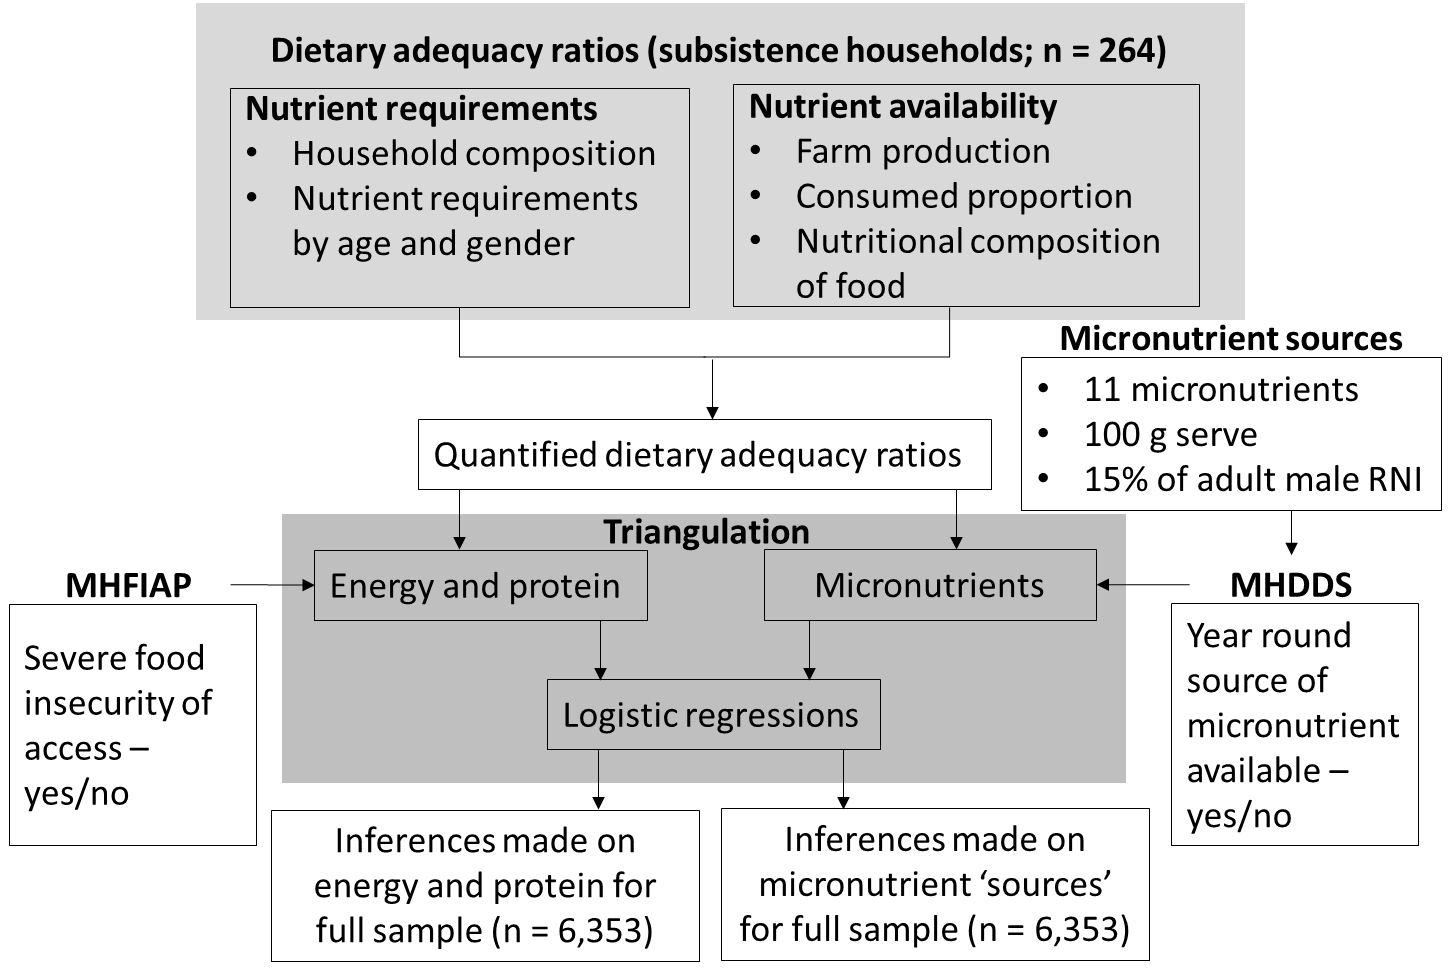
\includegraphics[width=1\textwidth]{figs_06/image1.png}
  \caption{Triangulation of dietary gaps. Dietary adequacy ratios are quantified as the difference between household nutrient requirements and nutrient availability. Sources of micronutrients are identified as food categories (MHDD) that contain at least 15\% of a daily adult male's Recommended Nutrient Intake (RNI). Micronutrient sources and severe food insecurity (MHFIAP) are retained in subsequent analyses if they are associated with their respective quantified gaps}
  \label{fig:06_1}
\end{figure}

The computation of household \textit{nutritional requirements} was based on three established estimates: energy requirements (\citealp{FoodandAgricuturalOrganization2001}), safe level of protein intake (\citealp{WHO2002}) and recommended nutrient intakes (RNI) of micronutrients (\citealp{FAO2004}). Energy requirements were based on gender, an assumed increase in weight/basal metabolic rate (BMR) with age, an assumed moderate physical activity level (PAL value between 1.7 and 1.99) and assumed good health. With these assumptions, the estimated kilocalorie requirement for an adult male between 25 and 50 was 2750 kcal and 2250 kcal for females. Protein intake requirements were based on age and gender categories for children and adolescents and weight for adults. Micronutrient RNIs were based on age and gender categories. The total household requirements for each of these nutrients were then calculated as the sum of requirements by gender and age requirements. Variations in nutritional requirements due to health status, level of activity and interactions between nutrients (e.g. vitamin D promoting calcium absorption) were not accounted for. These limitations may have resulted in underestimates of nutrient requirements for households with poor health status and those that are more active. The resulting quantified dietary adequacy ratios of subsistence households are presented as boxplots in Appendix Figures \ref{fig:A_1} and \ref{fig:A_2}.

Household \textit{nutrient availability} was computed using food consumption volumes, which were estimated using farmer reported details of crop and animal-sourced food production, and their estimated proportion consumed. Meat yield from farm slaughtered animals was estimated based on approximate live weights and carcass composition; all households were assumed to consume liver from the animals that they had slaughtered -- based on dietary preferences for liver and the need to maximise carcass utilisation. Milk yield (minus suckling) was estimated based on farmer estimates of average daily litres on a seasonal basis (flush and lean), with an assumed lactation length of 270 days. The \textit{nutrient availability} of farm-sourced foods was derived from food composition tables specific to Tanzania (n$_{\mathrm{food items}}$ = 62; \citealp{Lukmanji2008}) and supplemented with region-specific values (e.g. fonio millet in West Africa; \citealp{FAO2012}) and USDA food composition tables where necessary (n$_{\mathrm{food items}}$ = 34; \citealp{USDepartmentofAgricultureUSDA2017}). Zinc and iron content was adjusted based on an estimated high dietary phytate to zinc supply ratio (molar ratio {\textgreater} 20 in SSA; \citealp{Joy2014}; defined as high by \citealp{Brown2001}) and the common practice of fermenting cereals (i.e. reducing phytate content, resulting in improved bioavailability; \citealp{Nout2009}). Thus, the bioavailability of zinc was assumed to be `moderate', and a 10\% bioavailability was assumed for iron -- which was held constant across households. The inedible proportions of food items were removed from the nutrient estimate calculations based on United States Department of Agriculture (USDA) proportion values. Modelling was focused on the total availability of nutrients and so did not factor in discarded edible portions (food waste), nor food transformations (e.g. flour and oil).

The association was then assessed between household dietary adequacy ratios and dietary gaps identified through the MHDD and MHFIAP indicators. Severe food insecurity-- as identified in the MHFIAP indicator -- was considered as a proxy for energy and protein adequacy ratios. Gaps in micronutrient `sources' -- as identified through the MHDD indicator -- was compared with micronutrient adequacy ratios. To assess whether households had year-round daily sources of individual micronutrients, we first identified the micronutrients associated with each MHDD food category. A `source' food category of a given micronutrient was defined by having an average availability of at least 15\% of the daily RNI for an adult male per 100 g serve (\citealp{FAO1997}). The average availability per MHDD category was based on the weighted average nutrient composition of farm production (based on sampled households), on a country and (if data limitations required) a regional basis (i.e. East, central and West Africa). As an exception, dairy was assumed to be a source of calcium, with a 100 g serve estimated to meet 12\% of an adult male's daily requirements. In East Africa, for example, three food categories in the MHDD indicator are sources of five or more micronutrients: nuts and seeds; meat, fish poultry; and vitamin A rich vegetables (refer to Appendix Table \ref{tab:C_4} and Appendix Table \ref{tab:C_5}). In contrast, dairy and eggs only provided a limited number of micronutrients but were important sources of those that were less common, namely: calcium (dairy), vitamin A (eggs) and vitamin B12. We assessed whether households had at least one source in both the flush period and lean period and if so, the household was categorised as having a year-round source of that particular micronutrient; if not, they had a dietary gap for that micronutrient.

The statistical associations between quantified adequacy ratios and dietary gaps identified through indicators (gaps in MHDD `sources'; MHFIAP -- severely food insecure) were assessed using logistic regressions for subsistence households only. In this specification, a binary dependent variable (availability of nutrient source through MHDD/HFIAP indicators -- yes/no) was modelled with the corresponding adequacy ratio as the independent variable. Logistic regression was used in favour of alternative statistical approaches so that our decision rule on whether to include/exclude a nutrient in further analysis could incorporate the direction of association (expected to be positive) as well as the statistical significance of the association (expected to have a p-value of less than 0.05).

%Univariate post hoc regression outputs are summarised as coefficient and the probability ... t/z
\subsection{Associations between dietary gaps and livelihood characteristics}

The prevalence of dietary gaps were weighted based on population estimates of the administrative unit that the households were sampled to represent. Population estimates of the year 2015 were extracted from the `gridded population of the world' dataset (version 4; CIESIN, 2017) -- masking out densely populated areas (>1000 people per km$^2$). Observations were then weighted based on the average population density in the administrative unit (persons per km$^2$), relative to other administrative units -- such that each household within an administrative boundary was weighted equally and relative to other administrative boundaries. The weights of studies that only sampled livestock keeping households were adjusted, assuming that they represent 50\% of the rural population. The sum of weights equated to the sample size.

We model associations between nutrient gaps and household composition, farm production mix, market participation and income. Agroecological zone (AEZ) was also included as fixed effects in the regression models to control for the effects of differences between semi-arid locations (Length of growing period; LGP 75 -- 180 days) and humid/sub-humid locations (LGP {\textgreater} 181 days). We incorporated random effects on the intercept from villages nested within projects in our models. We used negative binomial regressions with mixed-effects to model overdispersed count variables (MHDD) and logistic regressions with mixed-effects to model whether households were severely food insecure (of access) or not and whether households have a gap in sources of micronutrients.

To further explore modelled associations, we developed a farm typology based on the composition of farm production -- which influences both cash availability and diversity of own-farm food availability (\citealp{Headey2018}; \citealp{Jones2016}). Farms were classified as `specialised cropping' if they reported two or fewer crop species as being important for their livelihood or sourced two or fewer plant-based food categories (e.g. `legumes' or `leafy vegetables') from their farm; farms with three or more crop species/plant-based categories were classified as having `diverse cultivation'. Livestock holdings (animals under the care of the household) were represented as Tropical Livestock Units (TLU), and households with over 1.5 TLUs (the equivalent of one head of cattle -- 1 TLU, one sow -- 0.3 TLU and five chickens -- 0.04 TLU) were categorised as having a livestock product (meat, milk or eggs) component to their farm, in combination with their cropping activities. This threshold was set marginally higher than one TLU to reduce instances of false positive classifications of households keeping an ox or donkey (0.8 TLU) for draught power purposes. We identified four distinct farm types: `Specialised cropping', `Diverse cropping', `Specialised cropping and livestock', and `Diverse cropping and livestock'. We use this farm typology to characterise channels of food access and to explore the prevalence of food insecurity and dietary gaps (Appendix Table \ref{tab:C_8} provides a regional breakdown of farm types.

Differences between farm types were modelled using mixed-effects linear and logistic regressions, with random effects on the intercept from villages nested within projects. Dependent variables of these models included farm-household characteristics, consumption behaviour and dietary gaps. The independent variable in these models was either farm type or an aggregation of farm types (e.g. livestock keeping). All regression models were estimated using a hybrid Monte-Carlo Markov Chain (MCMC) method, implemented in R using the `BRMS' package (v 1.0.1; \citealp{BuerknerP2016}). Weakly informative priors (Student's t-distribution with df = 5) were used, allowing extreme values but maintaining an expectation of minimal association (i.e. central tendency near zero). The posterior distributions were analysed and if 95\% of the density was above or below zero then it was considered to be significantly associated. Models were based on a core set of household and farm variables, with interactions tested additively. All regressions were weighted by population density -- minimising bias in generalisations to the sampled locations.


%Differences between farm types were modelled using mixed-effects linear and logistic regressions, with random effects on the intercept from villages nested within projects. Dependent variables of these models included farm-household characteristics, consumption behaviour and dietary gaps. The independent variable in these models was either farm type or an aggregation of farm types (e.g. livestock keeping). All linear and negative binomial regressions were performed using the lme4 package in R (\citealp{BatesD2017}). Linear regressions with non-parametric residuals were re-run with cuberoot transformed dependent variables. The statistical significance of fixed effects in linear regressions were assessed using the F-test with Kenward-Roger approximation (\citealp{Kenward1997}), comparing models additively from the intercept only model. All logistic regressions were performed with the glmmPQL function from the MASS package in R (\citealp{Venables2002}), which includes an overdispersion parameter to model the dependence between accumulated binary observations (\citealp{Breslow1993}). The statistical significance of fixed effects in the generalised linear regressions were assessed using the wald test using the aod package in R (\citealp{Lesnoff2012}).


\section{Results}

\subsection{Triangulation to identify energy, protein and micronutrient gaps}

Only 7 of the 11 micronutrients met our triangulation decision rules of statistical significance, a positive association (Table \ref{tab:06_1}). Thus, the nutrients included in the remainder of the results were limited to calcium, iron, thiamine, riboflavin, niacin, vitamin B6 and vitamin B12. Severe food insecurity (of access) in the lean period was associated with year-round energy and protein sufficiency and thus retained as a proxy to these dietary gaps.


\begin{table}[H]
  \captionsetup{singlelinecheck = false, justification=justified}
  \caption{
  Associations between quantified adequacy ratios and dietary gaps identified through indicators for subsistence households (n = 264). Nutritional elements with an inconsistency were excluded from further analyses (Logistic regression outputs -- beta coefficent estimate, standard error and statistical significance)
  }
  \label{tab:06_1}
  \small
\begin{tabular}{L{3cm} C{2.5cm} C{2cm} C{2cm}}
  %{
%p{\dimexpr 0.21\linewidth-2\tabcolsep}
%p{\dimexpr 0.26\linewidth-2\tabcolsep}
%p{\dimexpr 0.26\linewidth-2\tabcolsep}
%p{\dimexpr 0.26\linewidth-2\tabcolsep}}
\toprule
Nutrient & Estimate (SE) & Significance & Retained \\
\midrule
Energy & 1.00 (0.42) & * & x \\
Protein & 0.94 (0.40) & * & x \\
Calcium (Ca) & 2.78 (0.75) & * & x \\
Iron (Fe) & 0.84 (0.40) & * & x \\
Zinc (Zn) & 0.32 (0.41) & & \\
Vitamin A & 0.92 (0.46) & & \\
Thiamine & 0.96 (0.42) & * & x \\
Riboflavin & 0.95 (0.46) & * & x \\
Niacin & 0.94 (0.42) & * & x \\
Vitamin B6 & 0.80 (0.43) & * & x \\
Folate & -0.40 (0.40) & & \\
Vitamin B12 & 2.30 (0.57) & * & x \\
Vitamin C & -0.85 (0.54) & & \\
\bottomrule
\end{tabular}
\footnotesize
\raggedright
%\caption*{
\\
95\% CI does not cross zero\\
x = triangulation decision rules have been met
\end{table}



\subsection{Prevalence of severe food insecurity of access and dietary gaps}

Severe food insecurity (of access) was widespread across the surveyed households (\textit{n =} 6,353). In the lean period as many as 40\% of households were classified as severely food insecure according to the food access assessment with the HFIAP indicator. For micronutrients, 68\% of households did not have a year-round daily source of calcium, 38\% lacked a daily source of iron, 37\% lacked a daily source of thiamine, 51\% lacked a daily source of riboflavin, 44\% lacked a daily source of niacin, 35\% lacked a source of vitamin B6 and 65\% lacked a daily source of vitamin B12 (Table \ref{tab:06_2}).


\begin{table}[H]
  \setlength\dashlinedash{0.2pt}
  \setlength\dashlinegap{1.5pt}
  \setlength\arrayrulewidth{0.3pt}

  \captionsetup{singlelinecheck = false, justification=justified}
  \caption{Prevalence of dietary gaps weighted by population (n= 6,353; \% of weighted sample)}
  \label{tab:06_2}
  \small
\begin{tabular}{L{4.5cm} L{3cm} C{2.5cm}}
  %{\textwidth}{
%p{\dimexpr 0.44\linewidth-2\tabcolsep}
%p{\dimexpr 0.37\linewidth-2\tabcolsep}
%p{\dimexpr 0.19\linewidth-2\tabcolsep}}
\toprule
Proxy for dietary gap & Dietary requirement & Prevalence \\
\midrule
Severe food insecurity & Energy and protein & 40 \\
\arrayrulecolor{black!30}\midrule
%\hdashline
Source category accessed & Calcium (Ca) & 68 \\
daily throughout the year & Iron (Fe) & 38 \\
 & Thiamine (B1) & 37 \\
 & Riboflavin (B2) & 51 \\
 & Niacin (B3) & 44 \\
 & Vitamin B6 & 35 \\
 & Vitamin B12 & 65 \\
 \arrayrulecolor{black}\bottomrule
\end{tabular}
\end{table}

There are several factors associated with MHFIAP, MHDD and micronutrient sourcing (Table \ref{tab:06_3}). Regression results show that the number of household inhabitants was positively associated with diet diversity in the flush and lean periods as well as vitamin B12. The number of household inhabitants was also positively associated with the availability of year-round sources of thiamine and riboflavin in humid/subhumid zones. Female headed households were negatively associated with food security of access in the lean period and were less likely to have year-round sources of calcium. Having children under the age of 10 in the household was negatively associated with food security of access and diet diversity in the lean period, and negatively associated with having year-round sources of calcium and vitamin B12. These results suggest that there are household compositions with greater vulnerability to chronic and hidden hunger, which differs by AEZ in the instance of the number of household inhabitants.

Land cultivated was positively associated with having sources of calcium, iron, thiamine, and vitamin B6. However, in humid/subhumid zones land cultivated was negatively associated with access to sources of calcium. Livestock holdings were negatively associated with food security of access and diet diversity in the lean period. However, the association with diet diversity in the lean period was the weakest of all significant coefficients (Appendix Table \ref{tab:C_7}). Livestock holdings were also positively associated with diet diversity in the flush period (Figure \ref{fig:06_2}) and positively associated with the availability of sources for all micronutrients in both semi-arid and humid/sub-humid zones.

Market participation was positively associated with food security of access, diet diversity in both the flush and lean periods and positively associated with the availability of calcium, thiamine, riboflavin, vitamin B6 and vitamin B12. Off-farm income was positively associated with food security of access, diet diversity in both periods, as well as iron, thiamine, riboflavin, niacin, vitamin B6 and vitamin B12. Gross income was positively associated with food security of access, diet diversity in the flush and lean periods, and positively associated with the availability of sources of riboflavin and vitamin B12.

Crop production diversity was positively associated with food security of access in semi-arid zones, diet diversity in the flush and lean periods. In humid/subhumid zones, crop production diversity was negatively associated with food security of access. Crop production diversity was positively associated with the availability of iron, thiamine and niacin and negatively associated with calcium. The diversity of livestock products produced by a household was positively associated with food security of access, diet diversity in the lean period as well as being positively associated with calcium and vitamin B12. Livestock production diversity was negatively associated with iron, thiamine, and vitamin B6.

These results suggest that associations between diets and farm-household characteristics differ between AEZs. These differences between AEZs were most substantial for market participation and crop production diversity (full regression outputs shown in Appendix Table \ref{tab:C_7} and additional marginal effects presented in Appendix Figure \ref{fig:A_3}).


\begin{sidewaystable}
\centering
\captionsetup{singlelinecheck = false, justification=justified}
  \caption{
  Associations between nutrition (dependent variables in columns) and livelihood characteristics and agroecological zone (AEZ). Mixed-effects logistic\textasciicircum{} and negative binomial$^{\dag}$ regressions, displaying the direction of association for statistically significant explanatory variables (n = 6,353)
  }
  \label{tab:06_3}
  \small
  \centering
\begin{tabularx}{\textwidth}{
p{\dimexpr 0.29\linewidth-2\tabcolsep}
p{\dimexpr 0.08\linewidth-2\tabcolsep}
p{\dimexpr 0.07\linewidth-2\tabcolsep}
p{\dimexpr 0.08\linewidth-2\tabcolsep}
p{\dimexpr 0.04\linewidth-2\tabcolsep}
p{\dimexpr 0.04\linewidth-2\tabcolsep}
p{\dimexpr 0.08\linewidth-2\tabcolsep}
p{\dimexpr 0.09\linewidth-2\tabcolsep}
p{\dimexpr 0.06\linewidth-2\tabcolsep}
p{\dimexpr 0.07\linewidth-2\tabcolsep}
p{\dimexpr 0.07\linewidth-2\tabcolsep}}
\toprule
 & MHFIAP\textasciicircum{} & HDD flush period$^{\dag}$ & HDD lean period$^{\dag}$ & Ca\textasciicircum{} & Fe\textasciicircum{} & Thiamine\textasciicircum{} & Riboflavin\textasciicircum{} & Niacin\textasciicircum{} & Vitamin B6\textasciicircum{} & Vitamin B12\textasciicircum{} \\
 \midrule
Intercept &  & + &  & - & & & & & & - \\
Household inhabitants (adulteq.) &  & + & + & & & & & & & + \\
Female household head (yes) & - &  &  & - & & & & & & \\
Children under 10 (yes) & - &  & - & - & & & & & & \\
\arrayrulecolor{black!30}\midrule
Land cultivated (ha) &  &  &  & + & + & + & & & + & \\
Livestock holdings (TLU) & - & + & - & + & + & + & + & + & + & + \\
Market participation (\% kcal sold) & + & + & + & + & & + & + & & + & + \\
Off-farm income (yes) & + & + & + & & + & + & + & + & + & + \\
Gross income (PPP) & + & + & + & + & & & + & & & + \\
Crop production diversity${\ddag}$ & + &  & + & - & + & + & & + & & \\
Livestock product diversity${\ddag}$ & + & + & + & + & - & - & & & - & + \\
\arrayrulecolor{black!30}\midrule
AEZ (sub-)humid{\S} & + & + &  & + & - & - & + & & - & + \\
Household members:AEZ{\S} &  & + &  & & & + & + & & & \\
Land cultivated:AEZ{\S} &  &  &  & - & + & & & & & \\
Livestock holdings:AEZ{\S} &  &  &  & & + & & & & & \\
Market participation:AEZ{\S} & - &  &  & & & & & & & - \\
Crop production diversity:AEZ{\S} &  &  & + & & & & & + & + & \\
\arrayrulecolor{black}\bottomrule
\end{tabularx}
\footnotesize
\raggedright
%\caption*{
$^{\ddag}$Number of crop/livestock MHDD categories produced\\
$^{\S}$AEZ reference category = semi-arid\\
+ Statistically significant positive association; - statistically significant negative association

\end{sidewaystable}

\newpage



\begin{figure}[H]
  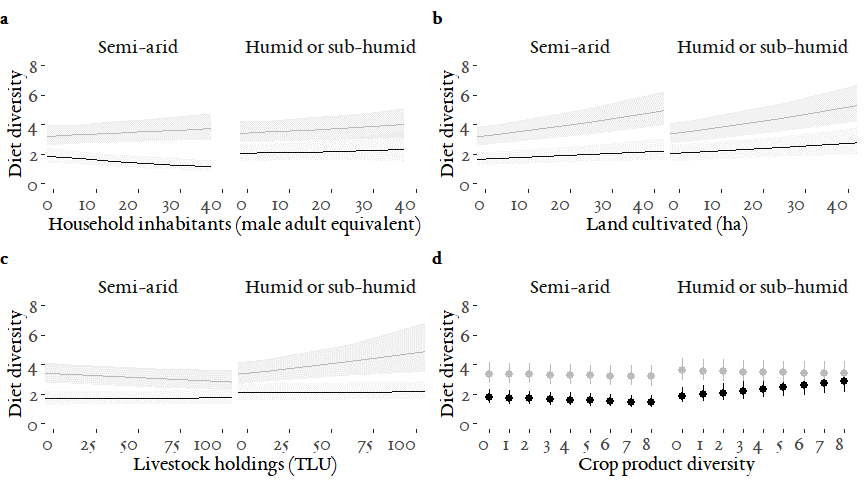
\includegraphics[width=1\textwidth]{figs_06/image2.png}
  \captionsetup{singlelinecheck = false, justification=justified}
  \caption{Predicted associations between MHDD and a) household inhabitants (adult eq), b) land cultivated, c) livestock holdings (Tropical Livestock Units), d) crop product diversity in the flush (grey line/point) and lean (black line/point) periods by agroecological zone}
  \label{fig:06_2}
\end{figure}

\subsection{Channel of food access and dietary gaps by farm type}

Households with a livestock component tended to have more people in the household, larger land area cultivated, better `progress out of poverty' and -- naturally -- more livestock (mixed-effects linear regressions; 95\% CI > 0; Appendix Table \ref{tab:C_11}). `Diverse cropping' and `Diverse cropping and livestock' households tended to have greater market participation than their specialised counterparts (mixed-effects linear regression; 95\% CI > 0; Appendix Table \ref{tab:C_12}). Farm types with a livestock component had significantly higher MHDD scores in the flush and lean periods compared to other farm types (Table \ref{tab:06_4}; mixed-effects linear regression; 95\% CI > 0; Appendix Table \ref{tab:C_11}). As expected, all farm types had higher median MHDD scores in the flush period, compared to the lean period.


\begin{table}[H]
  \captionsetup{singlelinecheck = false, justification=justified} %left justify caption
  \caption{
  Summary of resources, income and diet diversity of sampled households by farm type (number, proportion and median-IQR)
  }
  \label{tab:06_4}
  \small
\begin{tabularx}{\textwidth}{@{}lYYYY@{}}
%  {
%p{\dimexpr 0.29\linewidth-2\tabcolsep}
%p{\dimexpr 0.14\linewidth-2\tabcolsep}
%p{\dimexpr 0.15\linewidth-2\tabcolsep}
%p{\dimexpr 0.14\linewidth-2\tabcolsep}
%p{\dimexpr 0.15\linewidth-2\tabcolsep}
%p{\dimexpr 0.15\linewidth-2\tabcolsep}}
\toprule
 & Specialised cropping & Diverse cropping & Specialised cropping \& livestock & Diverse cropping \& livestock\\
 \midrule
n & 719 & 1596 & 1085 & 2943\\
Subsistence households (\%) & 4 & 4 & 5 & 4 \\
AEZ (Sub-)humid (\%) & 52 & 61 & 31 & 44 \\
Smallholders (\% ${\leq}$2 ha) & 44 & 39 & 34 & 32 \\
Mixed crop-livestock (\%) & 3 & 4 & 17 & 25 \\
Household members (adult equivalents) & 4.5 (3.4) & 4.9 (3.7) & 5.9 (4.2) & 5.9 (3.8)  \\
\arrayrulecolor{black!30}\midrule
Land cultivated (ha) & 1.06 (1.39) & 1.42 (1.62) & 2 (3.05) & 1.82 (3.19) \\
Livestock holdings (TLUs) & 0.2 (0.7) & 0.3 (0.8) & 7.6 (24.1) & 7.0 (10.3)  \\
Off-farm income (PPP$^{-1}$ year) & 0 (0) & 0 (30) & 0 (0) & 0 (150)  \\
Progress out of Poverty Index score & 33 (26) & 29 (40) & 41 (23) & 45 (26)  \\
Market participation (proportion kcal sold) & 0.03 (0.50) & 0.25 (0.55) & 0.05 (0.44) & 0.25 (0.49) \\
Crop income (PPP$^{-1}$ year) & 0 (210) & 86 (507) & 0 (47) & 65 (629)  \\
Live animal (PPP$^{-1}$ year) & 0 (0) & 0 (11) & 1 (128) & 3 (275)  \\
Livestock product income (PPP$^{-1}$ year) & 0 (9) & 0 (19) & 3 (195) & 69 (480)  \\
\arrayrulecolor{black!30}\midrule
Daily diet diversity -- flush period & 2 (2) & 4 (4) & 3 (2) & 4 (3) \\
Daily diet diversity -- lean period & 1 (2) & 1 (3) & 2 (2) & 2 (3)  \\
\arrayrulecolor{black}\bottomrule
\end{tabularx}
\footnotesize
\raggedright
%\caption*{

\end{table}

\vspace{-0.5cm}

The channel of accessing MHDD food categories differed by farm type. In Figure \ref{fig:06_3} two channels of access -- farm sourced and purchased -- and total diet diversity for the four farm types are presented for the lean period (equivalent results for the flush period are presented in Appendix Figure \ref{fig:A_4}).

In Figure \ref{fig:06_3}, the probability density function of the count of household diet diversity (MHDD) categories is presented as a black line on the lower half of each facet. The line indicates the probability that a household in a given farm type consumes a given number of categories (1-10). Each facet also presents the proportion of households that consume certain categories for a given count of MHDD. For example, in the top right-hand facet showing `Specialised cropping' and `total', the second pillar shows households with only two MHDD food categories, where the most common daily sourced food category was `grains, roots, tubers and plantains', followed by `leafy vegetables', `other vegetables' and then `legumes'. In contrast, since the far-right pillar shows households which consume all 10 food categories, the proportions of each are equal. {Figure \ref{fig:06_4}} allows comparison between farm types for a specific channel and within farm types, between channels. Inference from this figure is focused on the central mass of the probability density function -- generally between 1 and 5 MHDD categories.

\begin{figure}[H]
  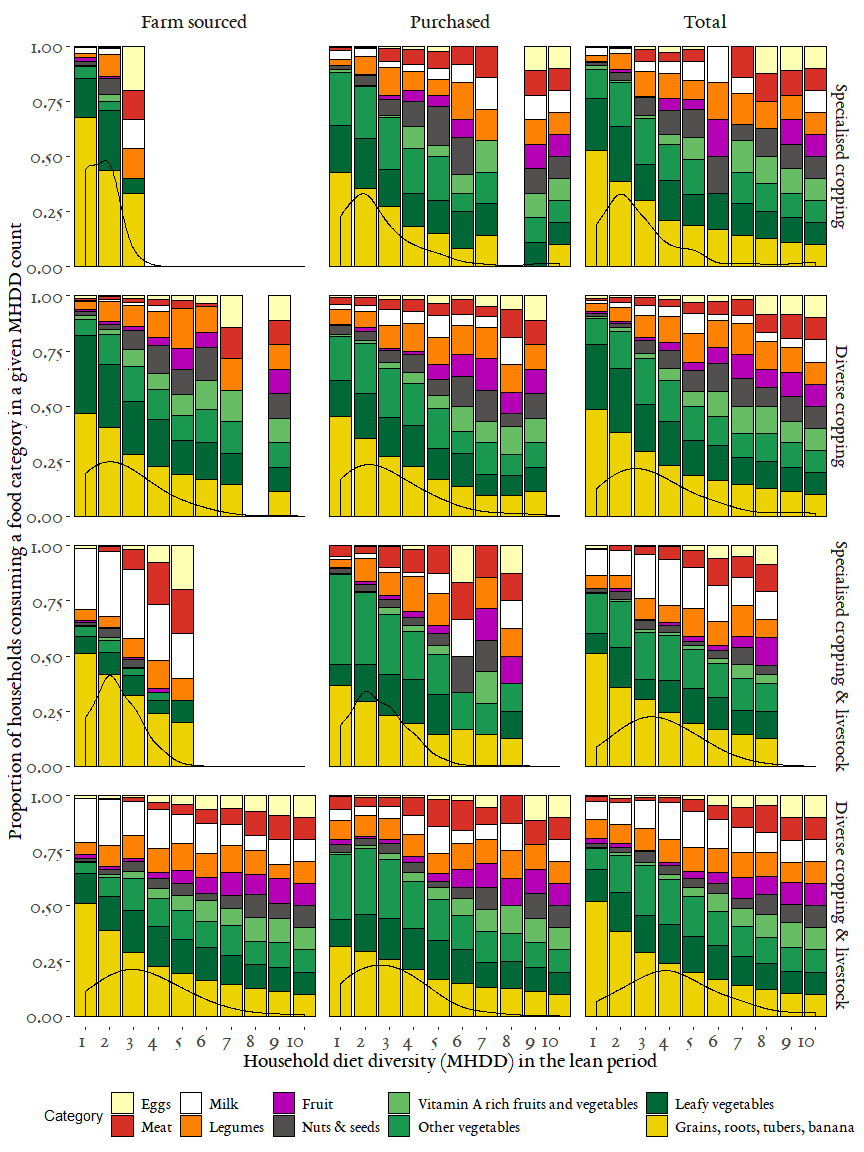
\includegraphics[width=1\textwidth]{figs_06/image3.png}
    \captionsetup{singlelinecheck = false, justification=justified}
  \caption{Diet diversity: density and proportion of sampled households (n=6,353) consuming specific food categories by farm type, channel of access and total diet diversity in the lean period. The distribution (probability density function) of diet diversity for each period is represented as a black line on the lower half of each figure facet. Food categories are represented by different colours, showing the proportion of households consuming each category at specific diet diversity levels}
  \label{fig:06_3}
\end{figure}

At the aggregate level, farm types with a substantial livestock component consume more livestock products -- milk, meat and eggs -- in both flush and lean periods (mixed-effects logistic regressions; 95\% CI > 0 for all animal source foods; Appendix Table \ref{tab:C_11}). In the lean period, 50\% of households with a livestock component to their farm consumed dairy products compared to less than 17\% of crop-oriented households. In Figure \ref{fig:06_3}, it is evident that dairy products are predominantly accessed through the farm channel and are sometimes the only daily sourced food category. Meat consumption -- a source of vitamin B12 among several other micronutrients -- in the lean period was marginally higher in households with a livestock component (38\% compared to 28\% of crop-based households). Meat was most often purchased, particularly in the flush period -- irrespective of farm type. Daily egg consumption -- also a source of vitamin B12 and riboflavin -- was less common, but consistently higher in households with a livestock component (results not tabulated elsewhere).

A greater proportion of households with a diverse cropping component to their farm tended to source plant-based food categories in the flush period -- except `nuts and seeds' and `grains, roots, tubers and banana' (mixed-effects logistic regressions;  95\% CI > 0 for all plant-based categories; Appendix Table \ref{tab:C_12}). In the lean period, when compared to other farm types, a smaller proportion of households in the `Specialised cropping' farm type sourced `legumes', `fruit', `vitamin A rich fruits and vegetables', and `other vegetables'.


The prevalence of severe food insecurity (of access) was not independent of farm type in both humid/sub-humid and semi-arid agroecological zones (Table \ref{tab:06_5}).

\begin{table}[H]
  \captionsetup{singlelinecheck = false, justification=justified}
  \caption{
  Associations between severe food insecurity, farm type and agroecological zone (AEZ). Mixed-effects logistic regression.
  }
  \label{tab:06_5}
  \small
\begin{tabular}{L{8cm} C{2.5cm} C{2cm} C{2cm}}

\toprule
 & estimate (SE) & Significance \\
\midrule
Intercept & -0.51 (0.91) &  \\
Diverse cropping$^\dag$ & -0.32 (0.16) & * \\
Specialised cropping \& livestock$^\dag$ & -0.92 (0.16) & * \\
Diverse cropping \& livestock$^\dag$ & -0.41 (0.17) & * \\
AEZ$^\ddag$ & 0.05 (0.12) & \\
\bottomrule
\end{tabular}
\footnotesize
\raggedright
%\caption*{
\\
95\% CI does not cross zero\\
$^\dag$Reference category is `Specialised cropping' \\
$^\ddag$Reference category is semi-arid
\end{table}

Specialised cropping households tended to have a higher prevalence of severe food insecurity -- when compared with all other farm types (Table \ref{tab:06_5}). In humid/sub-humid AEZs, households with `Diverse cropping \& livestock' had a lower prevalence of severe food insecurity and gaps in all micronutrients, when compared to other farm types (mixed-effects logistic regressions; 95\% CI > 0; Appendix Table \ref{tab:C_13_2}; Figure \ref{fig:06_4} and Appendix Figure \ref{fig:A_5}). In semi-arid zones, the difference between farm types was more distinct, where households with a livestock component to their farm had a significantly lower prevalence of calcium and vitamin B12 (mixed-effects logistic regressions; 95\% CI > 0 for MHFIAP and all micronutrients; Appendix Table \ref{tab:C_13_3}).

\begin{figure}[H]
  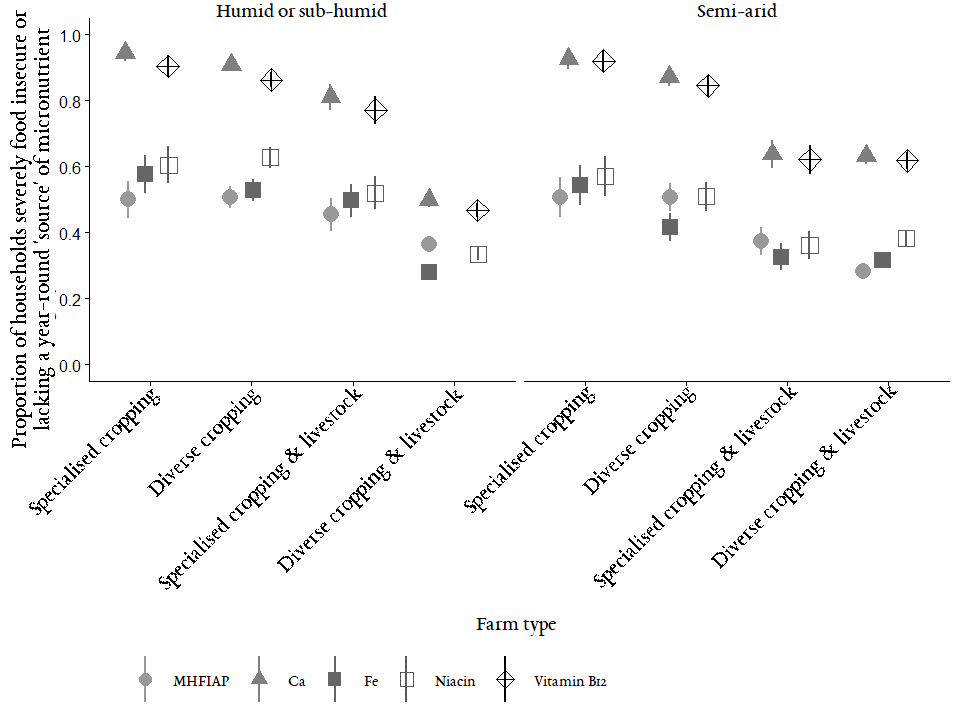
\includegraphics[width=1\textwidth]{figs_06/image4_weighted2.png}
  \captionsetup{singlelinecheck = false, justification=justified}
  \caption{Proportion of households (n = 6,353 weighted by population) with insecure access to food (MHFIAP) or no `source' of calcium, iron, niacin, or vitamin B12 by farm type and agroecological zone. A 95\% confidence interval is represented by vertical lines}
  \label{fig:06_4}
\end{figure}

\section{Discussion}

\subsection{Food insecurity and dietary gap prevalence}

The aim of this study was to combine diet diversity and food (in)security indicators with household-farm characteristics to estimate prevalence of dietary gaps and to understand their associations with rural livelihoods and food sourcing behaviour throughout the year. In addition to generating key information on food security of access and dietary diversity over the course of the year for a wide range of contrasting systems in sub-Saharan Africa, our approach also allowed us to quantify dietary gaps for six important micronutrients (Table \ref{tab:06_2}): calcium, iron, thiamine, riboflavin, niacin, vitamin B6 and vitamin B12.

The prevalence of dietary gaps in this study are comparable to previous studies, despite the substantial differences in target populations and sampling procedures. An estimated 40\% of sampled households were severely food insecure in their access to food; this is higher than reported by the FAO using the Food Insecurity Experience Scale (FIES; Appendix Table \ref{tab:C_10} provides a comparison of the questions asked) -- with an estimated 34\% of the SSA population being severely food insecure in 2017 (\citealp{FAO2018}). An estimated 68\% of households did not source calcium-rich food categories on a daily basis, which is between deficiency prevalence estimates derived from \citet[calculated as the inverse weighted average of the probability of adequacy -- Appendix Table \ref{tab:C_11}; calcium deficiency prevalence was 91\% of sampled women in Burkina faso, Mali and Uganda]{Martin-Prevel2015} and \citet[54\% of individuals in Africa]{Joy2014}. Our estimates of gaps in iron availability (38\% of households) are lower than the deficiency prevalence estimates in \citet[78\%]{Martin-Prevel2015}, but within the range of estimates in \citet[whose estimates range from 5\% assuming low bioavailability (10\% available), to 43\% for very low bio-availability (5\% available)]{Joy2014}. Our estimates for thiamine (37\%), riboflavin (51\%), niacin (44\%) and vitamin B6 (35\%) are comparable to estimates in \citet[thiamine 32\%, riboflavin 56\% and niacin 34\%, vitamin B6 26\%]{Martin-Prevel2015}. Additionally, an estimated 66\% of households did not source vitamin B12 rich food categories on a daily basis, which is more conservative than the deficiency prevalence estimates derived from \citet[93\% of sampled women]{Martin-Prevel2015}.

\subsection{Contextual factors for targeting nutrition-sensitive interventions}

There are several factors associated with food security of access, diet diversity and the daily sourcing of micronutrients. From the perspective of designing nutrition-sensitive agricultural interventions, we discuss a) contextual factors that can improve the targeting of interventions and b) factors that can form the basis of an intervention or be incorporated as a complementary intervention.

The contextual factors identified in this study are either not possible to change through agricultural interventions (AEZ and household composition), or relate to complex farmer/household decisions that are beyond the scope of current public and civil society interventions in SSA (farm scale and farm type). These contextual factors can be used as inputs into the intervention targeting decision-making process, where the aim is to maximise the potential for practice adoption and impact on well-being. On the basis of our results, we expect households with `female heads' and children under 10 years of age to have a higher likelihood of severe food insecurity in the lean period -- supporting the need for programmatic strategies on gender inclusion (\citealp{Mason2015}), as well as focusing on the first 1000 days of life (\citealp{DePee2017}). Similarly, households with small land cultivation areas can be targeted to counteract the tendency of limited access to micronutrient sources (land size has been linked to both chronic and hidden hunger; \citealp{Godecke2018}).

Understanding the existing production systems (farm types) of rural households within and between locations can inform more advanced intervention targeting decisions. For example, an intervening agent (e.g. government, NGO, etc.) may initially target their interventions based on AEZ, farm scale and sub-sector (e.g. dairy), and then in the advanced stages, design and target interventions based on the prevailing farm types. This approach can improve the suitability of interventions to existing conditions (i.e. by enhancement, diversification, or substitution; \citealp{Fiorella2016}) and therefore maximises adoption potential. This contextual factor also provides opportunities to improve the nutrition sensitivity of interventions. Our results show that prevalence rates differ by farm type and AEZ (Figure \ref{fig:06_4}). For example, households without a livestock component had high instances ({\textgreater}80\%) of gaps in calcium and vitamin B12 sources. Intervention packages can be developed to address such dietary gaps, targeting specific farm types in specific AEZs (\citealp{Hetherington2017}; \citealp{Mulmi2017}; \citealp{Hoddinott2012}). This is also reinforced by \citet{Carletto2015}, who review a series of studies showing that a household's agricultural production can directly influence the dietary patterns of household members, where the extent of impact depends on a variety of factors including location, commodities produced, and whether a household keeps livestock for direct consumption.

\subsection{Designing nutrition-sensitive interventions}

There are three factors identified in this study that could be incorporated in nutrition-sensitive agricultural orientated interventions. Increasing farm income (in-part through increasing market participation), improving off-farm employment opportunities (including along the agricultural value-chain; \citealp{Davis2017}) and diversifying production (crops, home garden and livestock products) each had positive effects on food security of access, dietary diversity, and thereby providing sources of micronutrients. These results are in line with the overview presented by \citet[p.~147]{Ruel2018}, stating that `production diversity and livestock ownership are consistently associated with household and dietary diversity and, when measured, with increased intake of essential micronutrients'. There are, however, instances of negative associations with these variables -- such as livestock holdings and diet diversity in the lean period. Extreme increases in income or production diversity (i.e. from the lowest end of the scale to the highest), however, is only predicted to increase diet diversity in the lean period by 1 or 2 food categories (Figure \ref{fig:06_2}). This limitation needs to be taken into account when designing and monitoring nutrition-sensitive interventions. Success may not be measured in leaps in diet diversity, but rather by adding specific food categories (in sufficient frequency and quantity) that provide micronutrient sources that would otherwise be lacking.

\subsection{How do farm types differ in food sourcing behaviour?}

Our results clearly demonstrate that sourcing of food categories was strongly related to farm type (Figure \ref{fig:06_3}). We found that the farm-based route to dietary diversity was extremely important: consumption of specific food groups is strongly linked to what farm households produce on-farm. This is a key finding because a substantial part of households that lacked an aspect of production diversity -- and thereby miss certain avenues in the farm-based route to dietary diversity -- did not choose to supplement their lack of production diversity with an equivalent diversity of purchased food categories. Households with a livestock component to their farm consumed more livestock products -- in-part due to their on-farm availability (also identified by \citealp{Hetherington2017}). Dairy, for example, was predominantly sourced from the farm in the lean period, where 50\% of households with a livestock component to their farm consumed dairy products compared to less than 17\% of crop-oriented households. Similarly, households with a diverse cropping component to their farm sourced a greater diversity of fruit and vegetable food categories (legumes, fruit, vitamin A rich produce, and other vegetables) -- mainly from the farm.

The finding that only a subset of households supplement gaps in production diversity with an equivalent diversity of purchased food categories indicates that extra income does not necessarily translate into food and nutrition security -- particularly for hidden hunger. Rather, dietary choices are -- in part -- driven by the retail environment, resulting in increased consumption of processed and sweetened foods (categorised as `grains, roots, tubers and banana'; `dairy'), increased instances of obesity and a higher burden of disease (\citealp{Demmler2018}; \citealp{GBD2016RiskFactorsCollaborators2017}; \citealp{Popkin2014}). Therefore, interventions aiming at improving dietary diversity through increasing incomes need to accompany their interventions with nutritional education to stimulate more diverse and nutritious purchases (\citealp{Dhanarajan2017}), or by stimulating production to improve local availability (globally, we lack sufficient fruit and vegetables for 22\% of the human population; \citealp{Siegel2014}). Otherwise, our results suggest that income-based interventions are unlikely to be nutrition-sensitive.

\subsection{Methodological considerations}

In this study we identified important associations between agricultural activities and pathways towards food security of access, diverse diets and gaps in micronutrient sources. These results, however, are limited by the means of data collection, the approximations made, the limited scope of analysis and the indicators used.

We used information collected in one-off (i.e. cross-sectional) household surveys, which are prone to non-credible values and reduced measurement precision. In total 1,355 observations (20\%) were removed from the original dataset -- largely due to missing MHDD data, as well as non-credible household or farm characteristics, and enumerator evaluated quality (Appendix Table \ref{tab:C_3}). Surveys were implemented using the same survey design, implimented with multi-stage clustered sampling strategies. The sampled households were more likely to be in lower socio-economic regions of rural SSA and so can not be taken to represent rural SSA as a whole. Population weightings were based on modelled data based on national statistics with variable quality.

The standard recall procedures of our food security indicators were adapted to enumerate both the lean and flush periods -- allowing us to capture the substantial variation of farm household diets throughout the year. This adaptation on the recall procedure, however, means that respondents may need to remember a set of circumstances from up to 11 months prior in order to answer a question -- potentially having a negative impact on measurement precision (\citealp{Beegle2012}).

The triangulation of energy, protein and micronutrients was based on a series of approximations on requirements and availability. These approximations were also based on data with known inaccuracies (\citealp{Joy2014}) and limited geographical representativeness (utilising food composition data from Tanzania and USDA). These challenges also plague more detailed dietary assessments across Africa (\citealp{Vila-real2018}) and will only improve if there are concerted efforts to generate high quality national and regional food composition tables across the continent. The triangulation is also limited by only assessing the dietary gaps in subsistence households; the diets of households that purchase foods may differ substantially in composition and quantity (\citealp{Popkin2014}). This limitation could be supplemented by information from country specific 24 hour recall datasets. Further work in using diet diversity indicators to assess micronutrient availability could also conduct sensitivity analyses to test the robustness of the triangulation procedure and the effect of farm classification on disaggregated diet gap prevalence.

Limiting our scope to the household level automatically limited the depth of the dietary gap analysis. This has consequences for the interpretation of results. For example, having a source of micronutrient as we have quantified in this study will have different implications for small households (likely to result in sufficiency) as opposed to larger households (they may access a micronutrient daily source but it is not enough for all members). Similarly, we naturally encounter the limitation for any household level indicator: it is not always clear whether we can translate household level findings into consequences for individual members of the family, for example: young children (\citealp{Caraher2016}).

In this study, we only assessed a limited set of indicators and associations. Although agriculture is a crucial determinant of food and nutrition security in landholding households, it is important to understand interactions with factors like education, gender, food preparation and sanitation to understand the full nutritional, and health consequences of our findings (in contrast, \citealp{Godecke2018} and \citealp{Ramankutty2018} do show associations with education and sanitation and \citealp{Dzanku2019} shows associations with gender). A substantial number of studies have reported the benefits of food security of access and a diverse diet on intermediary nutrition outcomes, such and child and maternal intake of ``target'' foods and micronutrients. Evidence of impact on nutrition outcomes -- particularly child anthropometry and micronutrient status -- was much more limited (\citealp{Gillespie2017}), stressing the limitations of using indicators like dietary diversity when inferring nutritional consequences (e.g. \citealp{Hetherington2017} showed weak and inconsistent associations between animal-source food consumption and anthropometric measurements).

Despite these inherent limitations of the analyses, we have quantitatively linked farming system characteristics to food and nutrition security indicators across a wide range of different production systems in sub-Saharan Africa. The most novel feature of this approach is that we can better understand how food security of access, diet diversity and micronutrient sourcing is related to the livelihood characteristics of a rural household over the course of a year (e.g. \citealp{Hammond2017225}). There is substantial variation in household diets, clear associations with livelihood characteristics and differences in food sourcing behaviour between farm types. These insights give confidence that simple approaches -- as used in RHOMIS -- can inform interventions at various levels to improve food and nutrition security in the diverse rural communities of SSA.

\section{Acknowledgments}

This research was made possible by several donors (listed in Appendix Table \ref{tab:C_1}). We would like to extend our gratitude to the rural households that participated in this research and the enumerators who guided the conversations.

\includepdf{ChapterPics/Ch7DiverseFood.png}
\chapter[General discussion]{General discussion}
\chaptermark{General discussion}
\label{cha:Chapter7}
\newpage

\section{Introduction}
The incidence of adverse health effects due to chronic undernourishment and micronutrient deficiencies are substantially higher in sub-Saharan Africa (SSA) compared to the rest of the world (\citealp{Godecke2018}). The individual and societal implications of this food insecurity are borne disproportionately by the rural SSA population (\citealp{Green2016}). Rural landholders are both vulnerable to the health burdens that stem from food insecurity, and central to improving the availability and affordability of a diversity of wholesome foods. To combat malnutrition, the global community needs to understand the interactions between food and nutrition (in)security and rural livelihoods. This understanding is currently missing.

The present understanding of food (in)security and rural livelihoods has been limited by the geographical and temporal scope of research efforts, and a lack of standardised rural household surveys. There is no one organisation with the resources to frequently monitor the vast diversity of rural communities at risk of food insecurity. Rather, rural household surveys are conducted nationally at in-frequent intervals and sub-nationally by a plethora of organisations. There have been considerable efforts to develop standardised rural household surveys over the past decade (e.g. \citealp{Carletto2009, Herrero2007}). However, these attempts to provide standardised survey designs have not resulted in substantial harmonisation and collaboration. \citet[p.~39]{Carletto2013} suggest that further harmonisation can be developed over time, with a ``combination of short-term fixes and long-term methodological advancements''. Recently, time-efficient proxies to food and nutrition security status have been developed -- marking a substantial methodological advancement (\citealp{Pisa2017, Keyzer2015}). These proxies can be readily incorporated into rural household surveys, providing comparable metrics across a diversity of studies to generate insights into the prevalence, spatial distribution and associations of food (in)security.

A growing body of literature utilising these food and nutrition security proxies has generated insights into the role that agricultural production and off-farm income plays in improving food and nutrition security. These findings, however, are dependent on the time of year that the survey is implemented and, have had a limited geographical scope -- limiting cross-site comparisons and more generalisable inference.

The primary objective of this thesis was to characterise food and nutrition security in rural landholding households in predominantly mixed crop-livestock agricultural systems of sub-Saharan Africa (SSA). Characterisation in this respect refers to describing the multiple facets of food and nutrition security, and identifying their associations with livelihoods. The secondary objective was to improve the methodological basis of household level food security studies.

This chapter first presents the research findings related to the harmonisation of rural household surveys to measure and monitor food and nutrition security. Harmonisation of rural household surveys is then discussed in terms of further methodological advances. A synthesis of findings related to food security and livelihoods is then provided. The discussion then continues with a focus on food and nutrition security in rural SSA in the context of nutrition-specific and nutrition-sensitive interventions; the stability of food and nutrition security throughout the year and; women's empowerment. The discussion then identifies further methodological advances for measuring food and nutrition security. This chapter is then concluded with a synthesis of findings.

\section{Harmonising rural household surveys}
\subsection{A balance between customisation and harmonisation}
A standardised rural household survey with an appeal to a wide user base was not available at the start of this PhD research. In a related PhD project, the rural household multi-indicator survey (RHOMIS) tool was developed to ``give a rapid, comprehensive overview of the farming system, which can be used to identify hotspot issues and to develop an evidence base to target deeper research'' (\citealp[P.~84]{Hammond2018}). Chapter 2 summarises this RHOMIS tool -- which was designed to collect a core set of modules, while being time-efficient, utilitarian, user-friendly, flexible and reliable (left-hand-side of Figure \ref{fig:07_1}). By being time-efficient, RHOMIS aims to minimise respondent fatigue and reduces the amount of time needed for survey design, implementation and analysis. The duration of the core set of modules in RHOMIS (listed in Figure \ref{fig:07_1}; provided in appendix 1 of \citealp{Hammond2018}) is estimated to be between 40 to 60 minutes (Table \ref{tab:02_1}). The duration of RHOMIS is half that of comparable surveys -- such as the `integrated modelling platform for mixed animal crop systems' (IMPACTlite; compared in Table \ref{tab:03_1}). The food availability indicator took the most time to collect, at a maximum of 35 minutes, followed by diet diversity, taking 10 minutes. The ease of enumeration was evaluated favourably for each module, with over 50\% of interviews being perceived as `easy' by the interviewer (Chapter 2).

The utilitarian design of RHOMIS means that every question is asked for a purpose. While this may sound logical, it is the norm in non-standardised household surveys to ask additional questions -- just in case they are important. In RHOMIS, each question is either incorporated into a composite indicator or used directly. If a variable or module proves to be ineffective, then it is revised or removed. The user-friendly principle of RHOMIS is most prominent in the design of the computer-aided personal interview (CAPI) system, which reduces the need for paper-and-pen entry. These design principles reduce survey time and respondent fatigue and provide efficiencies in data entry and data analysis.

The principle of flexibility refers to the extendibility and localisation of the survey. The core and additional modules are listed in Figure \ref{fig:07_1}, providing potential extensions into water, sanitation and hygiene (WASH), household expenditure and many more aspects of rural livelihoods. A survey needs to be adapted to the local language, units (standard measures of volume), foods and species. Over time, these localisations can be reused and improved upon. The RHOMIS tool is now available in 9 languages and has been localised to 48 sub-national locations in SSA, South-East Asia and South and Central America.

The credibility and consistency of data collected using RHOMIS was evaluated in Chapter 3. RHOMIS stayed within credible bounds more frequently than IMPACTlite and the Living Standards Measurement Study -- Integrated Survey on Agriculture (LSMS-ISA). The positive performance of RHOMIS in this respect could be attributed to the localisation of units -- minimising respondent estimation error. The inconsistency between IMPACTlite and RHOMIS (forming a test-retest study) was most evident in the diet diversity indicator. The limitations in dietary data collected in IMPACTlite may be explained by an unfortunate combination of poor question design and excessive survey duration. In contrast, the targeted questions in RHOMIS resulted in more realistic diet diversity estimates as there was less item non-response for commonly consumed food groups such as cereals and beans.

The design of RHOMIS has appealed to a diversity of users, including researchers and development organisations. The users of RHOMIS has evolved into a community of practice over the course of this PhD research. The RHOMIS community of practice has made substantial progress in harmonising data collection activities (www.rhomis.org). Throughout the duration of this PhD, the harmonisation of sampling, data pre-processing and testing of proxies was managed on a case-by-case basis (methodological developments listed in the top right of Figure \ref{fig:07_1}). These studies served as a proof of concept of effective rural household survey harmonisation. Now that there is an engaged community of practice, there are opportunities to make further methodological advances -- including introducing sampling guidelines, providing additional modules to validate indicators and introducing alternative modes of data collection (bottom right of Figure \ref{fig:07_1}). This section discusses each of these potential methodological advances.


\subsection{Further methodological advances for the RHOMIS approach}

\textit{Sampling support} was provided to organisations that did not have access to this support elsewhere. Rigorous sampling
is the basis of generalisable inference. All datasets utilised in Chapters 4 to 6 impliment multi-stage clustered sampling. Chapter 4 is based on geographically random sampling across villages within a 10-by-10 kilometre research area. Chapter 5 is based on purposively selected villages with random sampling from lists of households. Chapter 6 is based on several independent studies, sampling from lists of households within villages, but differing geographical bounds (e.g. Nationally representative and within a 10-by-10 km area). The consistency of sampling can be improved by providing \textit{sampling guidelines} that provide details on sample size determination (including reliability assessments -- Chapter 3) and various sampling methods (e.g. geographically random). The sampling method employed and suitable weightings would then be incorporated in the RHOMIS \textit{database} as \textit{meta-data}. This \textit{meta-data} would then allow the pooling of data-sets with similar sampling methods and geographical bounds.

There are also opportunities to critically assess the \textit{proxies} used in RHOMIS by \textit{validation} against more accurate methods. Specifically, in any given study, more detailed data can be gathered from a smaller subset of households to compare with the coarser measurement (referred to as `two-method measurement designs', \citealp{Little2013}). Validating proxies as well as meeting the primary research objectives is challenging to implement. It is particularly challenging to develop and implement two experimental designs -- one for the primary purpose of the research and another for the validation study. In the RHOMIS tool -- where much of the uncertainty of experimental design has been standardised -- an additional validation study is more tractable. Candidate variables for this process include: land size, diets, localisation units, crop yields and milk yield. By implementing two-method measurement designs, there is the potential to correct for errors in the broader dataset and identify methodological improvements.

\begin{figure}
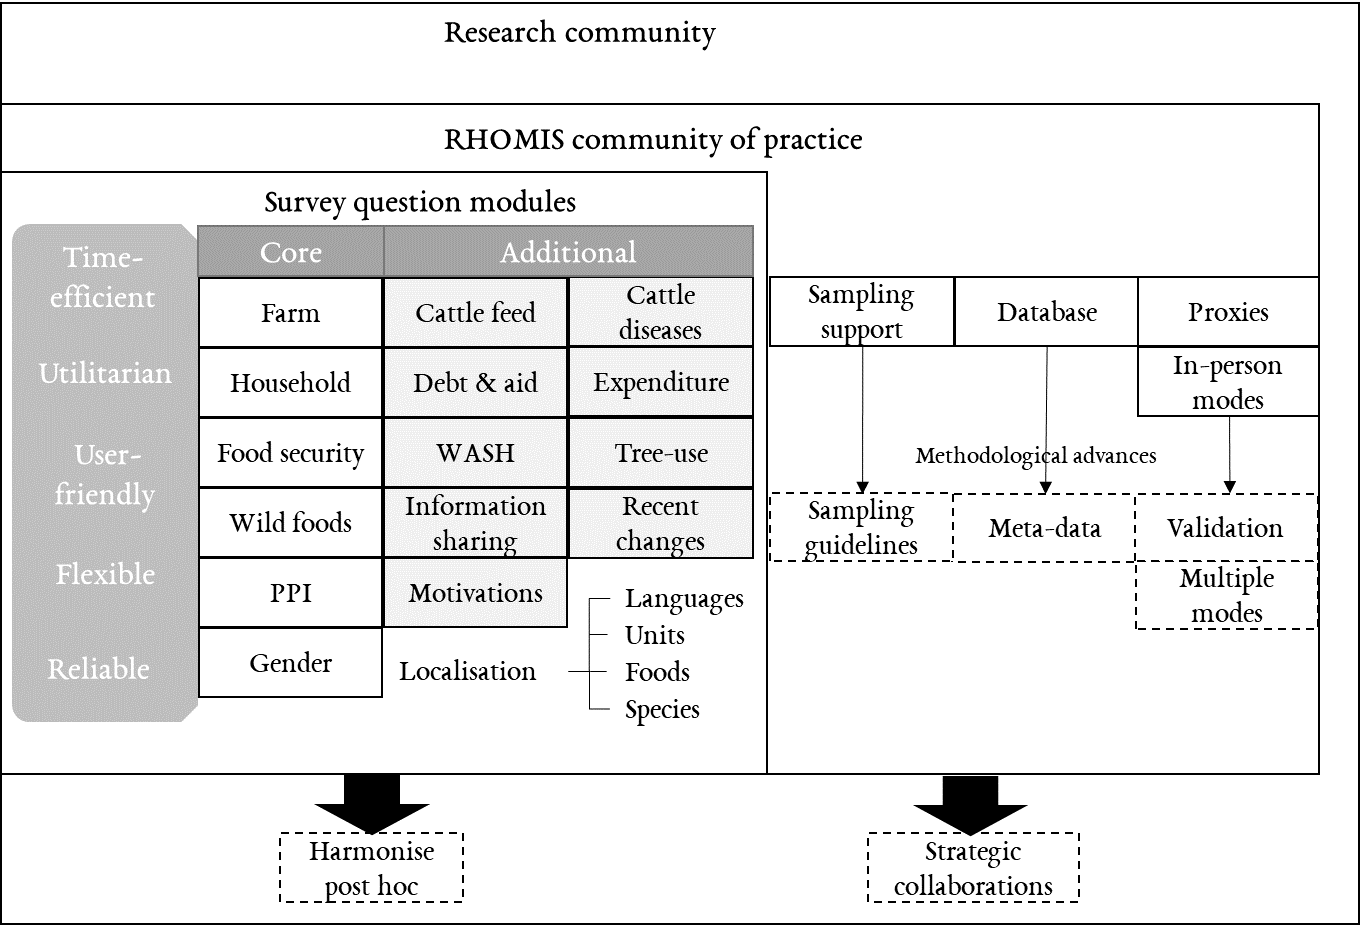
\includegraphics[width=1\textwidth]{figs_07/RHOMIS.png}
  \captionsetup{singlelinecheck = false, justification=justified} %left justify caption
  \caption{Summary of progress and pending developments to harmonise rural household surveys. Including the progress out of poverty index (PPI) and; water, sanitation and health (WASH) modules from the rural household multi-indicator survey}
  \label{fig:07_1}
\end{figure}

Research can also be explicitly carried out to validate indicators. In this instance, an experiment is designed to compare alternative indicators against a `gold standard'. An example of this would be to compare the modified household diet diversity recall periods (Chapters 5 and 6) to quarterly 24-hour dietary recall (24hR). Such a research effort could validate one of the alternatives, and potentially identify modifications that need to be made.

The RHOMIS tool has relied on \textit{in-person modes} of data collection with multiple recall periods. The reliance on multiple recall periods means that respondents may need to remember a set of circumstances from up to 11 months prior in order to answer a question -- having a negative impact on measurement precision (\citealp{Beegle2012}). In an initiative such as the RHOMIS community of practice, it is not possible to force users to revisit households multiple times throughout the year. Relying on recall has been a pragmatic reality.

As an alternative to multiple recall periods, \textit{multiple modes} of data collection can be used to build relationships with respondents in-person and then to follow-up with the same respondents in a cost effective manner. In particular, as 46\% of the SSA population is now connected to mobile networks there is the potential to engage rural households through the use of mobile phones (\citealp{GSMAIntelligence2016}). Short messaging services (SMS) and computer-assisted telephone interviewing (CATI) are two alternatives in this respect. In a comparison between face-to-face interviews (CAPI) and CATI, Lamanna et al. (accepted) found that telephone interviews were effective for the majority of questions asked. Sensitive questions on child and maternal health differed significantly by mode. There were also some mode effects at the food category level, with pulses reported more frequently in CATI and milk reported less frequently. These findings suggest that data collection through CATI can introduce biases. The cost of CATI interviews were reported to be US\$5 per successful survey, compared to US\$16 for face-to-face. One concern raised by Lamanna et al. (accepted) was that CATI may disproportionately exclude those less likely to have access to a mobile phone, such as the less wealthy and young women. Aside from the cost savings, this method has the potential to reduce recall period, and to improve the monitoring of communities in conflict zones (as in northern Yatenga -- Chapter 5) or communities that are geographically inaccessible.

In addition to methodological improvements, there are also opportunities to \textit{harmonise} RHOMIS data with other research efforts and to form strategic collaborations (bottom of Figure \ref{fig:07_1}). To-date, RHOMIS has been harmonised with other datasets, increasing the total number of observations from 25,000 to 50,000. Even with such a large database, there are still geographical and temporal gaps which can be addressed by forming \textit{strategic collaborations}, to harmonise with existing RHOMIS data. This can work by coordinating with specific organisations (e.g. UNICEF, CARE or World Vision) that are delivering projects in food insecure locations that currently lack harmonised data.

The harmonisation of rural household surveys is the result of more than a decade of steady progress. Rural households can now be characterised in a standardised way, enumerating multiple indicators of food and nutrition security. These indicators include: food availability, food security of access, diet diversity, food-self-sufficiency (adequacy ratios), sources of micronutrients and duration of food scarcity. This thesis draws on a total of 8,257 household interviews, conducted in 14 projects to characterise food and nutrition security in rural landholding households.

\section{Food and nutrition security in SSA}
\subsection{Prevalence and spatial heterogeneity of food insecurity}
In the sample of rural landholders across SSA, as many as 40\% of households were classified as severely food insecure in the `lean' period -- defined as the period of food scarcity. In general, households sourced two food categories on a daily basis in the `lean' period and three food categories in the `flush' period (median; results not shown). The implications of diet diversity on micronutrient deficiencies (hidden hunger) differed depending on which food categories were sourced. Disaggregating the count of diet diversity, it was reported in Chapter 6 that 68\% of households did not have a year-round daily source of calcium, 38\% lacked a daily source of iron, 37\% lacked a daily source of thiamine (vitamin B1), 51\% lacked a daily source of riboflavin (vitamin B2), 44\% lacked a daily source of niacin (Vitamin B3), 35\% lacked a daily source of pyridoxine (vitamin B6) and 65\% lacked a daily source of cobalamin (vitamin B12) (Table \ref{tab:06_2}). The prevalence of chronic and hidden hunger was highly variable between and within regions. Within-region variability is evident in Chapter 5, where households in two relatively similar provinces of Burkina Faso exhibited markedly different rates of food insecurity. More generally, instances of food insecurity differed by household composition, farm-business characteristics, income diversification and agro-ecological zone (AEZ; Chapter 6).

\subsection{Food and nutrition security and livelihoods}
Household composition was significantly associated with food security across sampled regions of rural SSA (Chapter 6). Female-headed households were more likely to be chronically hungry in the lean period and to lack sources of calcium -- where the head of the household is defined by asking in the initial stages of the interview. It was also the case that lower performing `subsisting' households identified in Chapter 4 were predominantly female-headed. Similarly, households with children under the age of 10 were more likely to be chronically hungry in the lean period, and more likely to lack sources of calcium (Table \ref{tab:06_3}). Households with children under the age of 10 tended to have more inhabitants, the same level of income, lower progress out of poverty and therefore higher instances of hunger (Appendix Table \ref{tab:C_14}). These findings support the need for programmatic strategies on gender inclusion (bottom right of Figure \ref{fig:07_3}; \citealp{Mason2015}), as well as the need for focusing on maternal and child nutrition (\citealp{Sharma2017, DePee2017, Arimond2004}). A livelihood in this thesis is defined as the way resources are utilised to maintain the wellbeing of an individual or social group (\citealp{Blaikie1994}). In Chapter 4, substantial changes in livelihoods were observed over three years -- suggesting that livelihoods are dynamic over a short period of time. Livelihoods were also observed to be highly variable (Chapters 4, 5 and 6). For example, Table \ref{tab:05_2} summarises two sites with relatively low production potential; within and between these sites there was substantial variation in household inhabitants, land area and livestock holdings. Despite this variability, several livelihood characteristics were identified to be associated with food security across sampled regions of SSA -- including size of land area, size of livestock holdings, production diversity, level of gross income and extent of income diversification -- i.e. earning off-farm income.

Households with larger land area cultivated were more likely to have more diverse diets. The effect of land cultivated on diet diversity was most substantial in the flush period. As livestock holdings increased, households were more likely to have access to sources of all micronutrients -- regardless of AEZ. The diversity of livestock products produced by a household, furthermore, was positively associated with food security of access, diet diversity in the lean period as well as being positively associated with calcium, iron, thiamine, niacin, vitamin B6 and vitamin B12 (Chapter 6). Crop production diversity was positively associated with food security of access and diet diversity regardless of AEZ. However, the association between crop production diversity and accessing sources of micronutrients differed by AEZ. Households in humid and sub-humid zones were more likely to access micronutrient sources as crop production diversity increased.

In reality, it is the combination of these livelihood characteristics that influences food security status. Chapter 6 identifies four distinct farm types, labelled: `Specialised cropping', `Diverse cropping', `Specialised cropping and livestock', and `Diverse cropping and livestock'. The prevalence of severe food insecurity and gaps in micronutrient sources depended on farm type. In humid and sub-humid AEZs, households with diverse crops had a lower prevalence of severe food insecurity. Additionally, `Diverse cropping \& livestock' households in humid and sub-humid zones had a lower prevalence of gaps in all micronutrients. In semi-arid zones, the difference between farm types was more distinct, where households with a livestock component to their farm had a lower prevalence of severe food insecurity and gaps in all micronutrients.

In this discussion, the higher performing farm types that keep livestock are further disaggregated by land area cultivated (Figure \ref{fig:07_2}). In humid and sub-humid zones, households labelled as `Diverse cropping medium-large' (n = 493) were less likely to be chronicly hungry and were more likely to have access to sources of calcium and niacin compared to their smallholder counterparts (n= 797; mixed-effects logistic regressions; 95\% CI < 0, Appendix Table \ref{tab:C_15}). In semi-arid zones, `Specialised cropping medium-large' (n = 402) were less likely to be chronicly hungry and were more likely to have access to sources of iron, thiamine, riboflavin, niacin and pyridoxine when compared to their smallholder counterparts (n = 343; mixed-effects logistic regressions; 95\% CI < 0; Appendix Table \ref{tab:C_16}). These results suggest that all the relevant interactions between livelihood characteristics are not fully captured in the modelling of Chapters 5 and 6. Rather, food security status is determined by the combination of land area, livestock holdings, production composition and land area -- differing by AEZ.

\begin{figure}[H]
\includegraphics[width=1\textwidth]{figs_07/prevalence_weighted2.png}
  \captionsetup{singlelinecheck = false, justification=justified} %left justify caption
  \caption{Proportion of livestock keeping households (n = 4,028 weighted by population) chronically hungry or lacking micronutrient `source' by farm type, scale and agroecological zone. A 95\% confidence interval is represented by vertical lines}
  \label{fig:07_2}
  \small

\end{figure}

Income diversification was also found to be associated with food security. In Chapter 4, households in Lushoto earning off-farm income in the `Rising high-value crops' cluster had significantly higher diet diversity in the flush period when compared to others in the cluster. In Chapter 5, households in northern Burkina Faso that earned off-farm income were less likely to be severely food insecure. Off-farm income had a significantly positive effect on diet diversity in Seno province as gross farm income increased. However, in Yatenga province, it was predicted that households not earning off-farm income had a greater potential to have more diverse diets. More generally across a diversity of rural communities of SSA, Chapter 6 showed that off-farm income was positively associated with food security of access, diet diversity, as well as calcium, riboflavin and vitamin B12. The difference between Chapter 5 and 6 in this respect suggests that off-farm income is positively associated with improved food security status in general, but can have differing effects at a site disaggregated level.

The associations between livelihoods and food security are mediated by food sourcing decisions. Households can access food from their own farm, through purchases or by trading, hunting or gathering. This thesis focused on two channels of food access, from own-farm production and purchased foods (presented as `own production' and `income' channels in Figure \ref{fig:07_3}). In northern Burkina Faso, own-farm sourcing had the potential to fulfil much of the household's energy needs, and the diversity of diets was most differentiated through purchased foods (Chapter 5). However, in an analysis of multiple sites across SSA, Chapter 6 demonstrates that households fail to purchase food categories that nutritionally complement their own agricultural production. This means that less production diverse households are less likely to access sources of specific micronutrients, such as calcium (dairy), vitamin A (vitamin A rich fruits and vegetables) and vitamin C (other fruits).

Multiple statistically significant associations were identified in this thesis. The causality of these associations could not be fully represented in the models of Chapters 5 and 6. For instance, household composition is associated with food security because headship and stage of life influence livelihood characteristics -- not due to a direct causal association. Several livelihood characteristics were associated with food security. It is the combination of these livelihood characteristics and agro-ecological production potential that drive the availability of food and income. Food security is then mediated by food sourcing decisions related to own-farm food availability and income availability. While purchases tend to drive overall diet diversity, a few select food categories are more readily sourced if available through the own-farm channel. These findings suggest that improving food security through rural livelihoods requires a focus on increasing supply, adding nutritional value through the own-farm channel and increasing demand for nutritious foods (relating to the three strategies of Figure \ref{fig:07_3}).

\section{Interventions, stability of food security and gender}
\subsection{Maximising the nutritional impact of interventions}
It has been estimated that much of the chronic and hidden hunger quantified in this thesis can be alleviated by implementing a set of \textit{nutrition-specific} interventions at a cost of US\$9.6 billion per annum -- including programs on fortification, micronutrient supplementation and exclusive breastfeeding promotion (\citealp{Bhutta2013}). It is emphasised in \citet[p.~452]{Bhutta2013} that if such expenditure is ``linked to \textit{nutrition-sensitive} approaches--i.e., women's empowerment, agriculture, food systems, education, employment, social protection, and safety nets--they can greatly accelerate progress in countries with the highest burden of maternal and child undernutrition and mortality.''. The implementation of \textit{nutrition-specific} interventions, in combination with \textit{nutrition-sensitive} interventions, calls for greater coordination between intervening agencies working across multiple disciplines.

The International Fund for Agricultural Development (IFAD) framework on nutrition-sensitive value-chains defines three strategies that encompass \textit{nutrition-sensitive} agricultural, food systems and education interventions -- namely, \textit{increase supply}, \textit{increase demand} and \textit{add nutritional value} (\citealp{DeLaPena2018}). Strategies to \textit{increase supply} (\citealp{Ruel2013}) aim to increase farm, regional and national food supply by improving productivity and reducing waste (top left box of Figure \ref{fig:07_3}). Strategies that \textit{increase demand} for nutritious food aim at product and nutritional education (bottom-left of Figure \ref{fig:07_3}). Strategies that \textit{add nutritional value} aim to improve the nutritional content of food produced, for example, by promoting vitamin A rich sweet potato; maintain the nutritive quality, for example through grain storage or refrigeration; and, \textit{improve food safety}, for example by reducing aflatoxin contamination. Several \textit{nutrition-specific} interventions also add nutritional value to the food system and so fall within the scope of the IFAD framework. The remainder of this subsection discusses \textit{increasing supply} and \textit{adding nutritional value}.

The framework acknowledges that \textit{increasing supply} and incomes will not directly improve nutritional status. Rather, individuals need to decide how the additional supply is to be utilised (`own-farm channel') and how income is to be spent (`income channel' in Figure \ref{fig:07_3}; \citealp{Price2018, Kazianga2017, Galie2015}). In fact, a concern of agencies implementing agricultural interventions is that the economics of productivity gains will drive increased specialisation and market orientation, which would reduce production diversity and compromise nutritional status (\citealp{Tscharntke2012}).


\begin{figure}[H]
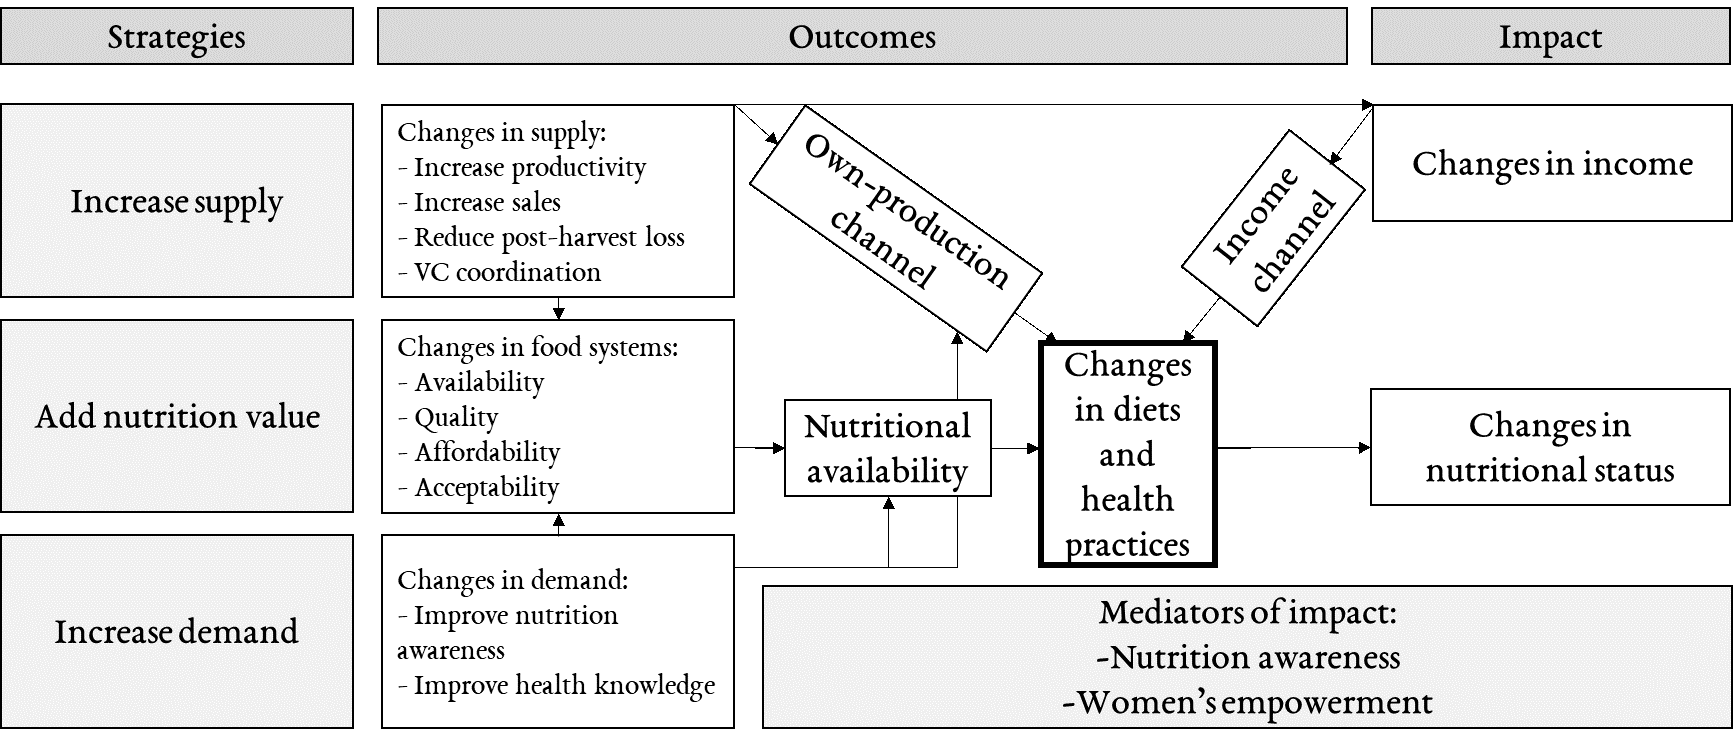
\includegraphics[width=1\textwidth]{figs_07/IFAD_frameworkv2.png}
  \captionsetup{singlelinecheck = false, justification=justified} %left justify caption
  \caption{Impact pathways of food system-based nutrition-specific and nutrition-sensitive interventions}
  \label{fig:07_3}
  %\small
  %\raggedright
  \vspace*{-3mm}
  \caption*{VC = value-chain \\
 	(Reproduced with permission from IFAD, 2018)}
\end{figure}



The literature indicates that there are several options for \textit{adding nutritional value} to food systems. Evidence suggests that interventions supporting livestock production can significantly reduce micronutrient deficiencies and health outcomes. For example, horticulture and poultry training has been found to increase vitamin A levels (\citealp{Masters2018}). Specifically, increasing animal-source food consumption has been found to significantly reduce stunting in low and middle-income countries (\citealp{Headey2018}).

The breeding and genetic modification of crops has also been a promising avenue to add nutritional value to food systems -- referred to as biofortification. Biofortification of pro-vitamin A crops (orange flesh sweet potato and maize; \citealp{Bouis2017}) and iron (beans and pearl millet) have been found to be effective physiologically and economically (\citealp{Osendarp2018}). For example, it has been estimated that interventions supporting sweet potato cultivation can save one disability average life year (DALY) for the cost of US\$15 -20 -- where a DALY is a standardised measure of human health and life expectancy (\citealp{Osendarp2018}). The biofortification of folate (B9) has also been tested in several crops and combined B vitamin biofortification is being explored (\citealp{Strobbe2018}).

Directly adding micronutrients to food systems has been identified as being one of the most cost-effective means of addressing hidden hunger (\citealp{Bhutta2013, Osendarp2018}). Referred to as fortification, this process adds specific micronutrients at safe levels to commonly consumed foods -- such as iodine to salt and bread, zinc and B vitamins to processed cereals, and vitamin D to foods with high oil content. Fortification is most commonly and cost-effectively implemented in collaboration with large-scale food processors. However, such processed foods may not be available to those at most risk to hidden hunger. In these instances, own-produced foods can be fortified by adding micronutrient powders -- referred to as complementary food production. Such complementary food production interventions-- have been effective at increasing iron and zinc intake in Ethiopia and Nigeria (\citealp{Masters2018}).

The implementation of agricultural-based interventions to \textit{add nutritional value}, however, is not as straightforward as fortification programs. As an example, \citet{Jenkins2018} identified a wide range of factors constraining adoption of orange flesh sweet potato in Mozambique -- including: taste preferences, availability of seed, and volatility of markets. To overcome the challenge of low adoption, programs can be designed as `packages', which combine agricultural and non-agricultural interventions, such as biofortified crops, complementary feeding, social safety-nets and women's empowerment (\citealp{Ruel2018, Jaenicke2013}). The micronutrient disaggregated analysis in Chapter 6 allows for the identification of potential dietary gaps of sub-populations, facilitating the targeting of such intervention packages. This packaging of interventions, however, requires greater collaboration between intervening agencies working across multiple disciplines, which is currently lacking.

There are several mediators to the effectiveness of nutrition-specific and nutrition-sensitive interventions. The following subsections discuss two mediators raised in this thesis, namely: the temporal variability of food and nutrition security, and the empowerment of women.

\subsection{Stability of food and nutrition security throughout the year}
The long-term stability of food and nutritional security is the ultimate goal of any effort to address chronic and hidden hunger. To support long-term stability, providing social protection and safety-nets have been identified as important \textit{nutrition-sensitive} interventions (\citealp{Bhutta2013}). An underlying challenge is that livelihoods are influenced by seasonal factors which determine the duration of scarcity, which tend to differ between and within AEZ. Figure \ref{fig:07_4} presents the variability in duration of food scarcity in Burkina Faso and Kenya, by AEZ.

In Burkina Faso, where the majority of households are located in semi-arid zones, over one-third of households experienced food scarcity in August (Figure \ref{fig:07_4}). In semi-arid zones of Burkina Faso, 63\% of households experienced between one and three months of food scarcity. In contrast, 48\% of households in humid and sub-humid zones did not experience any food scarcity months. The pattern of food scarcity months differed in Kenya, with households in semi-arid zones experiencing longer durations (2-6 months), later in the year (September-October) and households in humid and sub-humid zones experiencing shorter durations (2-4 months) earlier in the year (April). In the context of climate change and globalised markets, rural livelihoods are more exposed to climatic and market shocks, exposing households to the risk of more severe and longer food insecure periods (\citealp{Fanzo2018}).


\begin{figure}[H]
  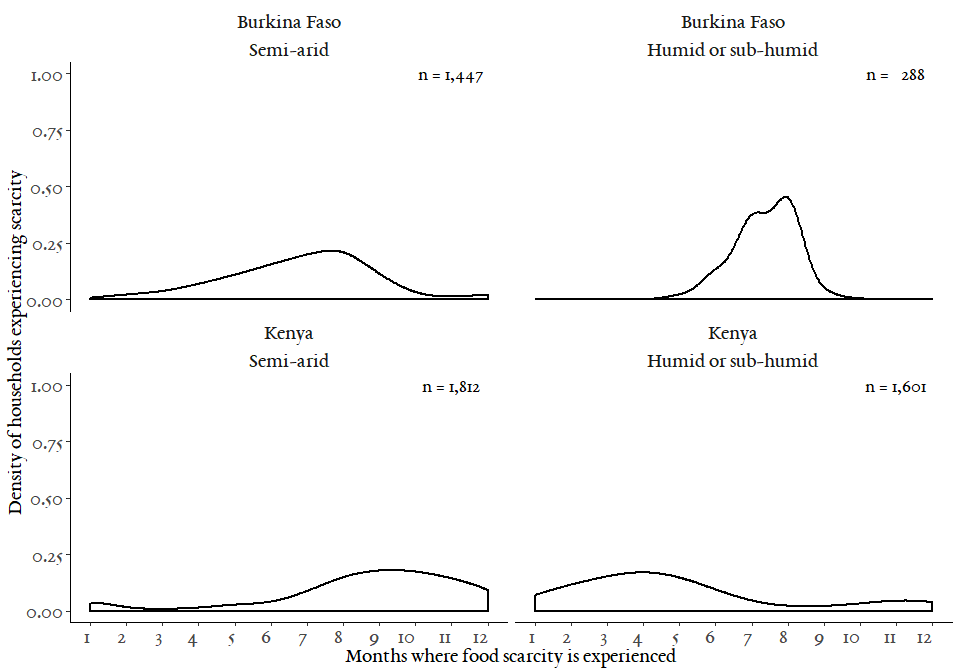
\includegraphics[width=1\textwidth]{figs_07/ScarceMonths_2.png}
  \captionsetup{singlelinecheck = false, justification=justified} %left justify caption
  \caption{Food scarcity months (January to December) of sampled households in Burkina Faso (n = 1070) and Kenya (n = 1030) sample by AEZ}
  \label{fig:07_4}
  %\small
  %\raggedright
  \vspace*{-3mm}
 	\caption*{(Observations from Chapter 6 only)}
\end{figure}

Increased exposure to climatic and market shocks have direct implications for the stability of food and nutrition security (\citealp{Ruel2018, Tomich2018, Jaenicke2013, Hussein1998}). Chapter 4 provides a case-study of households rapidly changing their climatic and market risk exposure. In Lushoto, Tanzania, households were found to be dynamic, making substantial changes to their farm over the course of three years. There appeared to be different approaches to market and climatic risks between the two higher performing clusters of households. The first cluster of households cultivated more land, with a portfolio of coffee, tomatoes, market vegetables, staples as well as keeping livestock species (agrobiodiverse production); the second cluster of households focused on livestock and staple crops. These differing production compositions have implications for risk exposure. Households in the first cluster may be less resilient to shocks in labour availability (e.g. due to ill health). Households in the second cluster may be more exposed to climatic and market risks due to a reliance on a limited range of crops and the absence of livestock. Notably, social safety-nets in the region have changed considerably over the past 30 years, where ``Access to unimproved subsistence land ... was still accepted as every resident's right... right up until the end of 1988'' (\citealp[p.~183]{Feierman1990}), and now safety-nets are based on family and social networks.

The role of agrobiodiversity (count of species) in the long-term stability of food and nutritional security was discussed in Chapter 5. While production diversity has a logical link with micronutrient sufficiency, the direct association with agrobiodiversity was weak (see also \citealp{Berti2015}). Rather, agrobiodiversity can co-exist with a market orientated strategy and provide risk management functions (\citealp{Waha2018a, Jaenicke2013, Tscharntke2012}). Livestock keeping -- as part of a diversified portfolio -- provides soil health benefits through the recycling of nutrients, as well as reducing livelihood risk by being a means to store capital (\citealp{Moll2005, Slingerland2000}). Similarly, diversified crop production can contribute to pest and disease management; reduce the market risk of volatile prices, and; can also be a part of a soil health strategy (e.g. nitrogen fixation or cover cropping to reduce erosion; \citealp{Lin2011}). Each of these benefits can reduce the risk exposure of a livelihood, specifically in relation to environmental or economic shocks. The packaging of interventions, therefore, would be appealing to production and income diversified rural households -- where they can adopt the most suitable innovations for their livelihoods.

\subsection{Women's empowerment and food security}
Land management, practice adoption and food access decisions are mediated by intra-household dynamics (Stirling, et al., submitted; Tavenner et al., submitted; \citealp{Dzanku2019, Price2018, AnderssonDjurfeldt2018a, Haider2018, Kazianga2017, Galie2015}). The empowerment of women -- in particular -- has been found to be central in changing diets and improving nutritional status (Figure \ref{fig:07_3}; \citealp{Rao2018, Price2018, Jaenicke2013}). As an extension of the analysis in Chapter 6, Table \ref{tab:07_1} presents a summary of households by gender of household head. In line with \citet{AnderssonDjurfeldt2018a}, these extended results suggest that there was a significant asset bias against female-headed households -- cultivating less land and owning fewer heads of cattle (Table \ref{tab:07_1}). Female-headed households exhibited a similar level of market participation to their male-headed counterparts. Despite this negative asset bias, female-headed households have comparable energy adequacy ratios from own-farm consumption, duration of scarcity and diet diversity in the lean period -- when compared to male-headed households (Table \ref{tab:07_1}). Chronic hunger, however, was found to be associated with female headship (Table \ref{tab:06_3}).
These findings indicate that the prevailing asset biases are the central areas for concern -- whether they be cultural or financial.

\begin{table}[H]
  \captionsetup{singlelinecheck = false, justification=justified} %left justify caption
   \caption{
    Livelihood characteristics and food security status by head of household (median; n = 6,343)
  }
  \label{tab:07_1}
  \small
  \centering
  \begin{tabularx}{\textwidth}{@{}lYYl@{}}  %{p{2cm}p{3cm}p{3cm}p{3cm}p{3cm}}
    \toprule
        &  Female headed & Male headed & $\beta_{female}$ (SE)  \\ %multirow spreads content over 3cm
        &(n=5,270)&(n=1,073)& \\
    \midrule

Household inhabitants (adult eq) & 4.4 (3.3) & 5.7 (4.1) & -0.86 (0.12)*$^\psi$\\
Land cultivated (ha) & 1.21 (1.40) & 1.62 (2.40) & -0.70 (0.20)*$^\psi$\\
Large ruminants (number) & 0 (4) & 1 (7) & -3.49 (1.08)*$^\psi$\\
Market participation (\% kcal sold) & 18 (0.48) & 23 (0.50) & -0.02 (0.01)*$^\psi$\\
Gross income (PPP) & 217 (946) & 254 (1,312) & 0.07 (8.31)$^\psi$\\
Progress out of poverty index (0 - 100)${\dag}$ & 38 (26) & 39 (28) & -0.59 (0.51)$^\psi$\\
Energy adequacy ratio (kcal consumed adult eq requirements$^{-1}$) & 0.42 (0.76) & 0.48 (0.81) &	-1.41 (1.18)$^\psi$\\
Length of lean period &	3 (3) &	2 (3) &	0.01 (0.02)$^\psi$\\
Diet diversity in the lean period (sourcing weekly) & 2 (3) & 2 (3) & -0.04 (0.07)$^\varphi$\\
    \bottomrule
  \end{tabularx}
  \footnotesize
  \raggedright
  %\caption*{
*\textbar95\% \textbar Credible Interval > 0; described in Chapters 5 \& 6\\
$^\psi$Linear regression. Random effects from villages nested within projects, weighted by population\\
$^\varphi$Negative binomial regression. Random effects from villages nested within projects, weighted by population\\
$^{PPP}$Purchasing power parity. See methods section of Chapter 6\\
$^\dag$Defined in Chapters 2, 3, 4, 5 \& 6

\end{table}

The differences between male-headed and female-headed households demonstrate that gender is an important mediating factor in accessing productive assets and therefore in mediating food security status. It is also expected that the empowerment of women will have an influence on food security within male-headed households (\citealp{Dzanku2019, Price2018, AnderssonDjurfeldt2018a}). Studies related to this thesis have used the RHOMIS database to identify associations between the empowerment of women and practice adoption (Stirling et al., submitted), as well as the empowerment of women and market orientation (Tavenner et al., submitted). To explore the role of gender in mediating food security empirically, we first calculated a gender equity indicator, quantifying gender disaggregated labour allocation, decision-making, asset ownership and control of income (Chapter 2). This indicator was used in exploratory analysis but was not found to be associated with the various food security indicators. This gender equity indicator was then disaggregated into labour allocation, decision-making, ownership of assets and control of income. Again, these metrics were not found to be associated with food security indicators. However, just because this thesis did not identify associations between food security and gender within male headed households, it does not negate the importance of gender. Rather, it may be a limitation of the quantitative indicator or the analytical approach used in this thesis.

Quantifying complex social dynamics in a cross-sectional interview is challenging. This challenge is compounded by the diversity of surveyed communities. The formulation of questions on labour allocation, decision making, ownership of assets and control of income can be standardised in a protocol and through enumerator training. For example, a protocol may specify question phrasing, such as: ``How much of the income from milk sales did you control? Where control means that you had full discretion to spend.''. However, in such a brief visit to a household, it is difficult to know exactly how the respondent interpreted such an intricate question. For example, one may have full autonomy to spend the income from milk sales, but social norms and power dynamics dictate the expenditure. Alternatively, the gender of the respondent may bias the answers given (\citealp{Tavenner2018}). The developers of the Women's Empowerment in Agriculture Index (WEAI) addressed these limitations by pre-testing the WEAI in several countries and running `cognitive testing' by language group and by interviewing men and women separately (\citealp{Malapit2015}). The resulting questions did inform the design of RHOMIS, but could not be incorporated in its entirety due to the risk of respondent fatigue (adding 30 to 60 minute duration for both the male and female respondent). In 2017, an Abbreviated Women's Empowerment in Agriculture Index (A-WEAI) was piloted, reducing survey time by 30\% (\citealp{Malapit2017}). Follow-up questions have also been introduced, such as: ``To what extent do you feel you can make your own personal decisions?''. The three A-WEAI modules currently not represented in RHOMIS are: leadership, group membership and detailed time allocation. These question revisions and modules could be piloted in future RHOMIS implementations. However, from the perspective of better understanding food security, the focus needs to be on labour allocation, decision making and income control. These aspects of gender dynamics will have a direct link with nutritional requirements, and food consumption and purchasing decisions. Indeed, the recent methodological advances in this domain may well provide the crucial empirical understanding needed to better design \textit{nutrition-sensitive} interventions.

\section{Further methodological advances for measuring food and nutrition security}
In this thesis multiple indicators were used to characterise food security and rural livelihoods. Indicators of food security included food availability, food security of access, diet diversity, food-self-sufficiency (adequacy ratios), sources of micronutrients and duration of food scarcity. The results of this thesis have implications for prioritising intervention beneficiaries, designing interventions and combining interventions into packages to meet the full nutritional needs of rural households throughout the year. Based on the progress in this thesis, there are a number of opportunities to improve methodologically. Specifically, further methodological advances can be made in the following areas: understanding intra-household dynamics; associating dietary proxies with nutrition and health; and, better quantifying dietary choices and obesity. These four developments can reduce the uncertainty around the associations identified in this thesis, and provide a richer understanding of food and nutrition security in rural landholding households.

Limiting our scope to the household level automatically constrained the depth of analysis. As such, it is not always clear whether we can translate household level findings into consequences for individual members of the family, for example, young children (\citealp{Caraher2016}). Enumerating at the individual level using the RHOMIS tool can be infeasible and result in additional error. Instead, households can be revisited for more in-depth studies. For example, Steinke et al. (submitted) conducted in-depth interviews with 15 high performing households from the database used in Chapter 6. In this study, Steinke et al. (submitted) found that these `positive deviants' tended to have one or more of the following traits -- \textit{meticulous} labour scheduling, \textit{collaborative} arrangements with neighbours and \textit{opportunistic} with small-scale off-farm business. Future in-depth studies could explore the intra-household dynamics of food and nutrition security -- including the role of gender and the provision of nutrition in the first 1000 days (\citealp{Sharma2017, DePee2017}).

In this thesis, we assessed a diverse but limited set of indicators and associations. Although agriculture is a crucial determinant of food and nutrition security in landholding households, it is important to understand interactions with factors like education, gender, breastfeeding practices, food preparation, nutritional supplementation, sanitation and instance of disease to understand the full nutritional, and health consequences of the findings. A substantial number of studies have reported the benefits of food security of access and a diverse diet on intermediary nutrition outcomes, such and child and maternal intake of `target' foods and micronutrients (e.g. \citealp{Some2018}; \citealp{Bellon2016}; \citealp{Koppmair2017325}; \citealp{Luckett20152479}; \citealp{Sibhatu201510657}; \citealp{Snapp2015}; and \citealp{Dillon2014}; \citealp{Siegel2014}). Evidence of impact on nutrition outcomes -- particularly child anthropometry and micronutrient status -- was much more limited (e.g. \citealp{Headey2018, Gillespie2017, Rah2010, Saha2009}), stressing the limitations of using indicators like dietary diversity when inferring nutritional consequences.

By enumerating broad food categories, this thesis has been constrained in assessing the quality of diets -- particularly from purchased foods. In part, dietary choices are driven by the retail environment, resulting in increased consumption of processed and sweetened foods (categorised as `grains, roots, tubers and banana'; `dairy'), increased instances of obesity and a higher burden of disease (\citealp{Demmler2018, GBD2016RiskFactorsCollaborators2017, Popkin2014}). With the rising burden of obesity, it will be important to better characterise purchased foods and consumption behaviour (Prentice, 2018). Such an evidence base will aid in the ambition to alleviate all forms of malnutrition.

\newpage
\section{Main conclusions}
This thesis sought to characterise food and nutrition security in rural landholding households of sub-Saharan Africa. The results of this thesis have implications for global efforts to alleviate chronic and hidden hunger.

\begin{itemize}
\item Agrobiodiversity can co-exist with a market orientated strategy and provide risk management functions.

\item	There was a high prevalence of chronic and hidden hunger, which was variable between and within regions.

\item	The gender of household head and stage of life influence livelihood characteristics (specifically resource availability), household requirements and thus food security. Several livelihood characteristics were identified to be associated with food security – including size of land area, size of livestock holdings, production diversity, level of gross income and extent of income diversification. It is the combination of these livelihood characteristics that influence food security status. The highest performing combination of livelihood characteristics differed by agro-ecological zone.

\item	Households fail to purchase food categories that nutritionally complement their own agricultural production. Therefore, improving food security through rural livelihoods requires nutrition-sensitive and nutrition specific interventions to increase supply, add nutritional value through the own-farm channel and increase demand for nutritious foods.

\item	Identifying dietary gaps of sub-populations can facilitate the targeting of interventions. Furthermore, programs can be designed as `packages' of agricultural and non-agricultural interventions to maximise adoption and impact.

\end{itemize}
% Discussion

\nocite{Lamanna, Stirling, Tavenner, Steinke} %Add submitted and accepted to reference list
%\nocite{*} %!To incude all references. Do this to make sure everything that should be cited in-text is actually in there

\backmatter %Remove chapter naming
%Bibs. See here https://en.wikibooks.org/wiki/LaTeX/More_Bibliographies
\bibliographystyle{model5-names} %Elsevier styles. Edited line 1007 to remove repetition of `doi:doi:'  %Changes all numnames to 200 so not truncated to et al. in bibliography
%Retreived from here: https://github.com/Sweitse/BibliographyStyles
%Alternatives: model2-names - excludes parentheses %!Other examples here %https://www.overleaf.com/learn/latex/Biblatex_bibliography_styles
%Or make your own style: https://ctan.org/tex-archive/macros/latex/contrib/custom-bib/


\bibliography{fullReferenceList} %! This is the bib file that you exported from Mendeley End note ect.
\addcontentsline{toc}{chapter}{References}
%For references at the end of each chapter, see this thread: https://tex.stackexchange.com/questions/87414/per-chapter-bibliographies-in-biblatex

\includepdf{ChapterPics/ChapterRefNandi.png}

\setcounter{table}{0}
\setcounter{figure}{0}
\renewcommand{\thetable}{A\arabic{table}}
\renewcommand{\thefigure}{A\arabic{figure}}

\chapter{Appendices}
\chaptermark{Appendix A}

\begin{sidewaystable}
%\begin{landscape}
 %\small
  %\begin{longtable}{lcccccccccccccccc}
  \captionsetup{singlelinecheck = false, justification=justified} %left justify caption
  \caption{Summary of selected sites, sampled households and agro-ecological zones (AEZ)}
  \label{tab:01_1}
  \small
  %\fontsize{7}{12}\selectfont%Very small font to fit table
\begin{tabular}{L{0.2cm} L{2.5cm} L{2cm} L{2cm} L{0.9cm} L{1cm} L{1cm} L{1cm} L{2cm} L{2cm} C{0.2cm} C{0.2cm} C{0.2cm} C{0.2cm} C{0.2cm}}
  %\begin{tabularx}
    %{\textwidth}{
  %p{\dimexpr 0.03\linewidth-2\tabcolsep}
  %p{\dimexpr 0.12\linewidth-2\tabcolsep}
  %p{\dimexpr 0.08\linewidth-2\tabcolsep}
  %p{\dimexpr 0.1\linewidth-2\tabcolsep}
  %p{\dimexpr 0.05\linewidth-2\tabcolsep}
  %p{\dimexpr 0.06\linewidth-2\tabcolsep}
  %p{\dimexpr 0.01\linewidth-2\tabcolsep}
  %p{\dimexpr 0.08\linewidth-2\tabcolsep}
  %p{\dimexpr 0.06\linewidth-2\tabcolsep}
  %p{\dimexpr 0.01\linewidth-2\tabcolsep}
  %p{\dimexpr 0.1\linewidth-2\tabcolsep}
  %p{\dimexpr 0.01\linewidth-2\tabcolsep}
  %p{\dimexpr 0.11\linewidth-2\tabcolsep}
  %p{\dimexpr 0.04\linewidth-2\tabcolsep}
  %p{\dimexpr 0.04\linewidth-2\tabcolsep}
  %p{\dimexpr 0.04\linewidth-2\tabcolsep}
  %p{\dimexpr 0.04\linewidth-2\tabcolsep}
  %p{\dimexpr 0.05\linewidth-2\tabcolsep}}
  \toprule
  ID & AEZ description* & Country & Site & Obs. & \multicolumn{3}{l}{Livelihood activities${\dag}$} & Market orientation${\dag}$ & Market Access${\dag}$ & \multicolumn{5}{l}{Thesis Chapter} \\
   & & & & & Dairy & Cash crops & Off-farm & & & 2 & 3 & 4 & 5 & 6 \\
   \midrule
  1 & Warm / semi-arid & Kenya & Makueni \& Kitui & 701 & & X & X & Low & Low & & & & & X \\
  2 & Warm / semi-arid & Mali & South-east & 363 & & X & & Unknown & Low & & & & & X \\
  3 & Warm / semi-arid & Tanzania & Various & 999 & X & X & X & Various & Various & & & & & X \\
  4 & Warm / semi-arid & Zambia & West & 624 & X & X & X & & & & & & & X \\
  5 & Warm / semi-arid & Kenya & Wote & 473 & X & X & X & High & High & & X & & & \\
  6 & Warm / semi-arid & Burkina Faso & Seno & 200 & &  & & Low & Low & & & & X & \\
  7 & Warm / semi-arid & Burkina Faso & Yatenga & 200 & & X & X & Moderate & Moderate & & & & X & \\
  8 & Warm / semi-arid & Burkina Faso & National & 763 & & X & X & Various & Various & & & & & X \\
  9 & Warm / sub-humid & Burkina Faso & National & 307 & & X & X & Various & Various & & & & & X \\
  10 & Warm / sub-humid & D.R. Congo & Central & 413 & & & X & Low & Low & & & & & X \\
  \bottomrule
  \end{tabular}
%\end{longtable}

\end{sidewaystable}
%\end{landscape}

\begin{sidewaystable}

  \small
  %\fontsize{7}{12}\selectfont%Very small font to fit table
  \begin{tabular}{L{0.2cm} L{2.5cm} L{2cm} L{2cm} L{0.9cm} L{1cm} L{1cm} L{1cm} L{2cm} L{2cm} C{0.2cm} C{0.2cm} C{0.2cm} C{0.2cm} C{0.2cm}}
  \toprule
  ID & AEZ description* & Country & Site & Obs. & \multicolumn{3}{l}{Livelihood activities${\dag}$} & Market orientation${\dag}$ & Market Access${\dag}$ & \multicolumn{5}{l}{Thesis Chapter} \\
   & & & & & Dairy & Cash crops & Off-farm & & & 2 & 3 & 4 & 5 & 6 \\
   \midrule
  11 & Warm / sub-humid & Tanzania & South-east & 522 & X & X & & Various & Various & & & & & X \\
  12 & Warm / humid & Kenya & Nyando & 160 & & X & X & Low & Moderate & & X & & & X \\
  13 & Cool / semi-arid & Ethiopia & Tigray & 250 & &  & & Low & Low & & & & & X \\
  14 & Cool / sub-humid & Ethiopia & Central highlands & 707 & X & X & X & Unknown & High & & & & & X \\
  15 & Cool / sub-humid & Tanzania & Lushoto & 149 & X & X & X & Moderate & Moderate & X & X & X & & \\
  16 & Cool / sub-humid & Tanzania & Mbeya & 560 & X & X & X & Low - moderate & Low - moderate & & & & & X \\
  17 & Cool / humid & Malawi & Makaika & 157 & & X & & High & Moderate & & & & & X \\
  18 & Cool / humid & Uganda & Rakai & 130 & & X & & Moderate & Moderate & & & & & X \\
  19 & Cool / humid & Kenya & Western & 169 & X & X & X & Moderate - high & Moderate & & & & & X \\
  20 & Various & Tanzania & & 841 & & X & X & Diverse & Diverse & & & & & X \\
  21 & Various & D.R. Congo & Eastern & 438 & X &  & X & Moderate & Low - moderate & & & & & X \\
  \bottomrule
  \end{tabular}
%\end{longtable}
\footnotesize
\raggedright *Sources: IFPRI, 2010 USAID, FEWS NET
\end{sidewaystable}


\begin{table}
  \captionsetup{singlelinecheck = false, justification=justified}
  \caption{
  Association between farm-household characteristics and survey year. Mixed-effects linear regressions.
  }
  \label{tab:A_1}
  \small
\begin{tabular}{L{5cm} C{2.5cm} C{2.5cm} C{2cm} C{2cm}}
\toprule
Dependent variable & Intercept estimate (SE) & $\beta_{2015}$ estimate (SE)$^\dag$ & $\beta_{2015}$ sig \\
\midrule
Land owned & 0.82 (0.08) & 0.26 (0.10) & ** \\
Crop diversity & 4.50 (0.17) & -1.28 (0.23) & *** \\
Crop income (USD$^1/3$) & 55.14 (7.85) & 18.66 (9.36) & * \\
\bottomrule
\end{tabular}
\footnotesize
\raggedright
%\caption*{
\\
*P {\textless} 0.05 \\
**P {\textless} 0.01 \\
***P {\textless} 0.001 \\
$^\dag$Reference category is 2012
\end{table}


\begin{table}
  \captionsetup{singlelinecheck = false, justification=justified}
  \caption{
  Association between farm-household characteristics and gender of household head. Mixed-effects linear regressions.
  }
  \label{tab:A_2}
  \small
\begin{tabular}{L{5cm} C{2.5cm} C{2.5cm} C{2cm} C{2cm}}
\toprule
Dependent variable & Intercept estimate (SE) & $\beta_{female}$ estimate (SE)$^\dag$ & $\beta_{female}$ sig \\
\midrule
Land owned & 1.07 (0.11) & -0.44 (0.17) & * \\
Livestock holdings (TLU) & 2.10 (0.23) & -1.27 (0.37) & *** \\
\bottomrule
\end{tabular}
\footnotesize
\raggedright
%\caption*{
\\
*P {\textless} 0.05 \\
**P {\textless} 0.01 \\
***P {\textless} 0.001 \\
$^\dag$Reference category is `male'
\end{table}

\begin{table}
  \captionsetup{singlelinecheck = false, justification=justified}
  \caption{
  Association between farm-household characteristics and gender of household head in `Subsisting mixed' households. Mixed-effects linear regressions.
  }
  \label{tab:A_3}
  \small
\begin{tabular}{L{5cm} C{2.5cm} C{2.5cm} C{2cm} C{2cm}}
\toprule
Dependent variable & Intercept estimate (SE) & $\beta_{female}$ estimate (SE)$^\dag$ & $\beta_{female}$ sig \\
\midrule
Land owned & 0.96 (0.12) & -0.37 (0.23) & NS \\
Livestock holdings (TLU) & 2.03 (0.19) & -0.85 (0.37) & * \\
\bottomrule
\end{tabular}
\footnotesize
\raggedright
%\caption*{
\\
*P {\textless} 0.05 \\
$^\dag$Reference category is `male'
\end{table}

\begin{table}
  \captionsetup{singlelinecheck = false, justification=justified}
  \caption{
  Association of food security indicators and farm type -- `Subsisting' vs. `Rising'. Mixed-effects regressions.
  }
  \label{tab:A_4}
  \small
\begin{tabular}{L{5cm} C{2.5cm} C{2.5cm} C{2cm} C{2cm}}
\toprule
Dependent variable & Intercept estimate (SE) & $\beta_{Rising}$ estimate (SE)$^\dag$ & $\beta_{Rising}$ sig \\
\midrule
Food availability (kcal adult equivalent$^{-1}$ day$^{-1}$) & 435 (45) & 287 (134) & ** \\
Household Diet Diversity Score in flush period$^\ddag$ & 2.10 (0.04) & 0.11 (0.05) & * \\
Household Diet Diversity Score in lean period$^\ddag$ & 1.67 (0.05) & 0.09 (0.08) &  \\
\bottomrule
\end{tabular}
\footnotesize
\raggedright
%\caption*{
\\
*P {\textless} 0.05 \\
**P {\textless} 0.01 \\
$^\dag$Reference category is `Subsisting' households
$^\ddag$Negative binomial regression
\end{table}


\setcounter{table}{0}
\setcounter{figure}{0}
\renewcommand{\thetable}{B\arabic{table}}
\renewcommand{\thefigure}{B\arabic{figure}}

%\chapter*{Appendix B}%The star removes the entry from the bibliography - add manually for the reading version
\textbf{Appendix B}
\chaptermark{Appendix B}

\begin{table}[H]
  \captionsetup{singlelinecheck = false, justification=justified}
  \caption{Food security of access by period and by province (\% of site)}
  \label{tab:B1}
  \small
\begin{tabularx}{\textwidth}{@{}llYYYY@{}}
%  {
%p{\dimexpr 0.30\linewidth-2\tabcolsep}
%p{\dimexpr 0.19\linewidth-2\tabcolsep}
%p{\dimexpr 0.13\linewidth-2\tabcolsep}
%p{\dimexpr 0.12\linewidth-2\tabcolsep}
%p{\dimexpr 0.14\linewidth-2\tabcolsep}
%p{\dimexpr 0.12\linewidth-2\tabcolsep}}
\toprule
 & & Food secure & Mildly food insecure & Moderately food insecure & Severely food insecure \\
 \midrule
Lean period & Seno & 1.5 & 2 & 13 & 83.5 \\
 & Yatenga & 10.5 & 17 & 41 & 31.5 \\
Flush period & Seno & 22 & 11 & 18 & 49 \\
 & Yatenga & 14.5 & 45 & 24 & 16.5 \\
 \bottomrule
\end{tabularx}
\end{table}

\begin{table}[H]
  \captionsetup{singlelinecheck = false, justification=justified}
  \caption{Intensification practices adopted in Seno for the 2015 cropping period (\% of households)}
  \label{tab:B2}
  \small
\begin{tabularx}{\textwidth}{@{}lYY@{}}
%  {
%p{\dimexpr 0.51\linewidth-2\tabcolsep}
%p{\dimexpr 0.25\linewidth-2\tabcolsep}
%p{\dimexpr 0.24\linewidth-2\tabcolsep}}
\toprule
 & Adopted & Not adopted \\
 \midrule
Improved livestock breeds & 1 & 99 \\
Value addition$^{\mathrm{a}}$ & 76 & 24 \\
Irrigate cash crops & 6 & 94 \\
Fertiliser & 20.5 & 79.5 \\
Improved seed & 31.5 & 68.5 \\
\bottomrule
\end{tabularx}
\footnotesize
\raggedright
$^a$Value addition of crops such as dehusking, hulling, polishing, milling ect.
\end{table}

\begin{table}[H]
  \captionsetup{singlelinecheck = false, justification=justified}
  \caption{Intensification practices adopted in Yatenga for the 2015 cropping period (\% of households)}
  \label{tab:B3}
  \small
\begin{tabularx}{\textwidth}{@{}lYY@{}}
  %{\textwidth}{
%p{\dimexpr 0.51\linewidth-2\tabcolsep}
%p{\dimexpr 0.25\linewidth-2\tabcolsep}
%p{\dimexpr 0.24\linewidth-2\tabcolsep}}
\toprule
 & Adopted & Not adopted \\
 \midrule
Improved livestock breeds & 0.5 & 99.5 \\
Value addition & 87.5 & 12.5 \\
Irrigate cash crops & 27.5 & 72.5 \\
Fertiliser & 39.5 & 60.5 \\
Improved seed & 62.0 & 38.0 \\
\bottomrule
\end{tabularx}
\end{table}


\setcounter{table}{0}
\setcounter{figure}{0}
\renewcommand{\thetable}{C\arabic{table}}
\renewcommand{\thefigure}{C\arabic{figure}}

%\chapter*{Appendix C}
\textbf{Appendix C}
\chaptermark{Appendix C}

\begin{table}[H]
  \captionsetup{singlelinecheck = false, justification=justified}
\caption{Summary of funding sources}
\label{tab:C_1}
\small
\begin{tabularx}{\textwidth}{@{}ll@{}}
  \toprule
  Acronym & Full name\\
  \midrule
  AVCD & Accelerated Value Chain Development\\
  BMGF & Bill and Melinda Gates Foundation\\
  CCAFS & Climate Change, Agriculture and Food Security\\
  CLiP & Crop-Livestock integration Project\\
  DI & Darwin Initiative\\
  FORETS & FOrmation, Recherche, Environnement dans la TShopo\\
  EU & European Union\\
  LSHTM-IMMANA & The London School of Hygiene \& Tropical Medicine --\\
   & Innovative Metrics and Methods for Agriculture Nutrition Action\\
  SAIRLA & Sustainable Agricultural Intesification Research and Learning in Africa\\
  SIDA & Swedish International Development Agency\\
  USAID & U.S. Agency for International Development\\
\bottomrule
\end{tabularx}
\end{table}

\vspace*{\fill}

%\newpage

\begin{sidewaystable}[ph!]
  \captionsetup{singlelinecheck = false, justification=justified}
  \caption{Summary of household data sources}
  \label{tab:C_2}
  \small
\begin{tabularx}{\textwidth}{
p{\dimexpr 0.26\linewidth-2\tabcolsep}
p{\dimexpr 0.15\linewidth-2\tabcolsep}
p{\dimexpr 0.15\linewidth-2\tabcolsep}
p{\dimexpr 0.21\linewidth-2\tabcolsep}
p{\dimexpr 0.13\linewidth-2\tabcolsep}
p{\dimexpr 0.11\linewidth-2\tabcolsep}}
\toprule
Country (site/region) & Donor & Project & Lead Institute implementing & Year & Number of Households surveyed \\
\midrule
Burkina Faso (country-wide) & SIDA & TreeAID & TreeAID-ILRI & 2018 & 1070 \\
DRC (Yangambi) & EU, CIFOR & FORETS & ICRAF & 2017 & 413 \\
DRC (Kamanyola \& Miti) & IFAD-EU & CLiP & IITA-ILRI & 2017 & 438 \\
Ethiopia (central highlands) & DI & TreeAID & TreeAID-ILRI & 2017 & 707 \\
Ethiopia (Tigray) & DFID & SAIRLA & Bioversity International & 2017 & 253 \\
Kenya (Makueni) & DFID & SAIRLA & Bioversity International & 2017 & 316 \\
Kenya (Nyando) & Maize CRP & CCAFS -- Maize & ILRI & 2016 & 161 \\
Kenya (Baringo \& Kitui) & DFID, LSHTM- IMMANA & SCAN & ICRAF & 2017 & 385 \\
Kenya (Busia, Homa bay, Siaya \& Vihiga) & USAID & AVCD & ILRI & 2017 & 169 \\
Kenya (Wote) & Maize CRP & CCAFS -- Maize & ILRI & 2016 & 160 \\
Malawi (Lilongwe area) & CCAFS & CCAFS & CIMMYT & 2015 & 157 \\
Mali (Diora, Mafoune \& Mandiakuy) & DI & TreeAID & TreeAID-ILRI & 2017 & 363 \\
Tanzania (country-wide) & USAID/BMGF & I4I Galvmed & ILRI & 2017 & 999 \\
Tanzania (incl. Zanzibar) & USDA-FAS & CSA & ICRAF & 2016 & 841 \\
Tanzania (Mtwara \& Lindi) & DFID & SAIRLA & Bioversity International & 2017 & 522 \\
Uganda (Rakai) & CCAFS & CCAFS & Wageningen University & 2017 & 130 \\
Zambia (3 districts) & DFID, LSHTM & SCAN & ICRAF & 2017 & 624 \\
\bottomrule
\end{tabularx}
\end{sidewaystable}

\newpage


\begin{table}[H]
  \captionsetup{singlelinecheck = false, justification=justified}
  \caption{Thresholds for removing observations (removed households may exceed multiple thresholds)}
  \label{tab:C_3}
  \small
\begin{tabularx}{\textwidth}{@{}lYY@{}}
  %{
%p{\dimexpr 0.48\linewidth-2\tabcolsep}
%p{\dimexpr 0.22\linewidth-2\tabcolsep}
%p{\dimexpr 0.29\linewidth-2\tabcolsep}}
\toprule
Variable & Threshold & Number of observations \\
\midrule
Household members (adult equivalents) & {\textgreater} 30 & 48 \\
 & = 0 & 68 \\
Land area (ha) & {\textgreater} 100 & 9 \\
Livestock holdings (TLUs) & {\textgreater} 250 & 72 \\
Income (PPP) & {\textgreater}100,000 & 93 \\
Modified Household Diet Diversity & = 0 & 776 \\
Enumerator assessed reliability & Regular doubts & 25 \\
 & Occasional doubts & 200 \\
Enumerator assessed ease to build rapport & Very difficult & 26 \\
\bottomrule
\end{tabularx}
\end{table}

%\smallskip
%\vspace{1cm}

Observations were removed in instances where no MHDD was enumerated or where land cultivated, livestock holdings or household population were non-credible (n = 1,355). Approximately 10\% of observations were removed from Burkina Faso, Kenya and Tanzania. After removing these observations, 6,612 households remained in this study.


\newpage

\begin{table}[H]
  \captionsetup{singlelinecheck = false, justification=justified}
  \caption{Sources of micronutrients in Modified Household Diet Diversity categories in East Africa (source defined as providing 15\% of adult male requirement)}
  \label{tab:C_4}
  \small
\begin{tabularx}{\textwidth}{@{}lYYYYYYYYYYY@{}}
%  {
%p{\dimexpr 0.19\linewidth-2\tabcolsep}
%p{\dimexpr 0.05\linewidth-2\tabcolsep}
%p{\dimexpr 0.04\linewidth-2\tabcolsep}
%p{\dimexpr 0.06\linewidth-2\tabcolsep}
%p{\dimexpr 0.07\linewidth-2\tabcolsep}
%p{\dimexpr 0.09\linewidth-2\tabcolsep}
%p{\dimexpr 0.09\linewidth-2\tabcolsep}
%p{\dimexpr 0.08\linewidth-2\tabcolsep}
%p{\dimexpr 0.08\linewidth-2\tabcolsep}
%p{\dimexpr 0.08\linewidth-2\tabcolsep}
%p{\dimexpr 0.09\linewidth-2\tabcolsep}
%p{\dimexpr 0.07\linewidth-2\tabcolsep}}
\toprule
~ & Ca${\dag}$ & Fe & Zn & VitA & Thiamine & Riboflavin & Niacin & Vitamin B6 & Folate & Vitamin B12 & Vitamin C \\
\midrule
Grains, roots, tubers and plantain & & x & & & x & & x & x & & & \\
Pulses & & & & & & & & x & x & & \\
Nuts and seeds & x & x & x & & x & x & x & x & x & & \\
Dairy & x & & & & & & & & & x & \\
Meat, poultry and fish & & & x & x & & x & x & x & & x & \\
Eggs & & & & x & & x & & & & x & \\
Leafy vegetables & & & & x & & & & & & & x \\
Vitamin A rich vegetables & & x & x & x & x & & & & & & x \\
Other vegetables & & & & & & & & & & & \\
Other fruits & & & & & & & & & & & x \\
\bottomrule
\end{tabularx}
\footnotesize
\raggedright
$^{\dag}$Threshold set at 12\%
\end{table}



\begin{table}[H]
  \small
  \raggedright Table \ref{tab:C_4} continued
\begin{tabularx}{\textwidth}%{@{}lYYYYYYYY@{}}
  {
p{\dimexpr 0.26\linewidth-2\tabcolsep}
p{\dimexpr 0.06\linewidth-2\tabcolsep}
p{\dimexpr 0.07\linewidth-2\tabcolsep}
p{\dimexpr 0.07\linewidth-2\tabcolsep}
p{\dimexpr 0.07\linewidth-2\tabcolsep}
p{\dimexpr 0.1\linewidth-2\tabcolsep}
p{\dimexpr 0.14\linewidth-2\tabcolsep}
p{\dimexpr 0.12\linewidth-2\tabcolsep}
p{\dimexpr 0.1\linewidth-2\tabcolsep}}
\toprule
~ & Cu & K & Mg & Mn & P & Pantothenic acid & Vitamin D & Vitamin E \\
\midrule
Grains, roots, tubers and plantain & & & x & x & x & & & \\
Pulses & & & & & & & & \\
Nuts and seeds & x & x & x & x & x & x & & x \\
Dairy & & & & & x & & & \\
Meat, poultry and fish & & & & & x & & & \\
Eggs & & & & & x & x & x & \\
Leafy vegetables & & & & & & & & \\
Vitamin A rich fruits and vegetables & x & & x & x & x & & & x \\
Other vegetables & & & & & & & & \\
Other fruits & & & & & & & & \\
\bottomrule
\end{tabularx}
\end{table}




\begin{table}[H]
  \captionsetup{singlelinecheck = false, justification=justified}
  \caption{Sources of micronutrients in Modified Household Diet Diversity categories in Central and West Africa (source defined as providing 15\% of adult male requirement)}
  \label{tab:C_5}
  \small
\begin{tabularx}{\textwidth}%{@{}lYYYYYYYYYYY@{}}
  {
p{\dimexpr 0.19\linewidth-2\tabcolsep}
p{\dimexpr 0.05\linewidth-2\tabcolsep}
p{\dimexpr 0.04\linewidth-2\tabcolsep}
p{\dimexpr 0.06\linewidth-2\tabcolsep}
p{\dimexpr 0.07\linewidth-2\tabcolsep}
p{\dimexpr 0.09\linewidth-2\tabcolsep}
p{\dimexpr 0.09\linewidth-2\tabcolsep}
p{\dimexpr 0.08\linewidth-2\tabcolsep}
p{\dimexpr 0.08\linewidth-2\tabcolsep}
p{\dimexpr 0.08\linewidth-2\tabcolsep}
p{\dimexpr 0.09\linewidth-2\tabcolsep}
p{\dimexpr 0.07\linewidth-2\tabcolsep}}
\toprule
~ & Ca${\dag}$ & Fe & Zn & VitA & Thiamine & Riboflavin & Niacin & Vitamin B6 & Folate & Vitamin B12 & Vitamin C \\
\midrule
Grains, roots, tubers and plantain & & x & & & x & & & x & & & \\
Pulses & & x & x & & x & x & & x & x & & \\
Nuts and seeds & x & x & x & & x & & x & x & x & & \\
Dairy & x & & & & & x & & & & x & \\
Meat, poultry and fish & & x & x & x & x & x & x & x & & x & \\
Eggs & & & & x & & x & & & & x & \\
Leafy vegetables & & & & x & & & & & x & & x \\
Vitamin A rich vegetables & & x & & & x & & & & & & x \\
Other vegetables & & & & & & & & & & & x \\
Other fruits & & & & & & & & & & & x \\
\bottomrule
\end{tabularx}
\footnotesize
\raggedright
$^{\dag}$Threshold set at 12\%
\end{table}

\begin{table}[H]
  \small
  \raggedright Table \ref{tab:C_5} continued
\begin{tabularx}{\textwidth}%{@{}lYYYYYYYY@{}}
  {
p{\dimexpr 0.26\linewidth-2\tabcolsep}
p{\dimexpr 0.06\linewidth-2\tabcolsep}
p{\dimexpr 0.07\linewidth-2\tabcolsep}
p{\dimexpr 0.07\linewidth-2\tabcolsep}
p{\dimexpr 0.07\linewidth-2\tabcolsep}
p{\dimexpr 0.1\linewidth-2\tabcolsep}
p{\dimexpr 0.14\linewidth-2\tabcolsep}
p{\dimexpr 0.12\linewidth-2\tabcolsep}
p{\dimexpr 0.1\linewidth-2\tabcolsep}}
\toprule
~ & Cu & K & Mg & Mn & P & Pantothenic acid & Vitamin D & Vitamin E \\
\midrule
Grains, roots, tubers and plantain & & & x & x & x & & & \\
Pulses & x & x & x & x & x & x & & \\
Nuts and seeds & x & x & x & x & x & x & & x \\
Dairy & & & & & x & & & \\
Meat, poultry and fish & & & & & x & x & x & \\
Eggs & & & & & x & x & x & \\
Leafy vegetables & & & & & & & & x \\
Vitamin A rich fruits and vegetables & & & x & x & & & & \\
Other vegetables & & & & & & & & \\
Other fruits & & & & & & & & \\
\bottomrule
\end{tabularx}
\end{table}

\vspace*{\fill}



%\newpage

%\vspace*{\fill}

The quantified adequacy ratios among subsistence households (n = 264) varied substantially by nutrient (\ref{fig:A_1} and \ref{fig:A_2}). There were consistently large gaps in the availability of vitamin A and vitamin C. Conversely, there were no micronutrient requirements that were consistently sufficient for all subsistence households.

\begin{figure}[H]
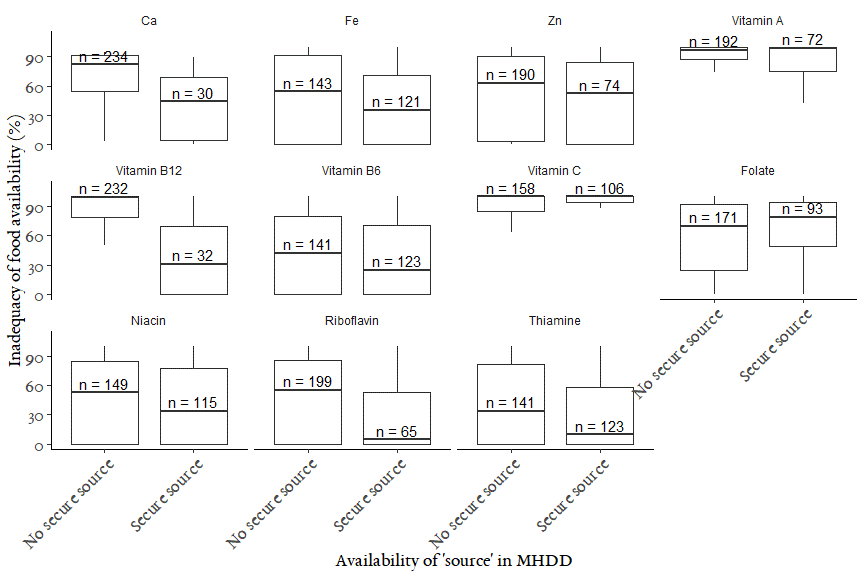
\includegraphics[width=1\textwidth]{Appendix/Ch6_1.png}
  \captionsetup{singlelinecheck = false, justification=justified} %left justify caption
  \caption{Comparison of all micronutrient gaps from farm production (y axis) and `sources' in the Modified Household Diet Diversity (MHDD) indicator (x axis). This figure is limited to farm dependent households. The `n' above the median line is the number of farm dependent households. A `secure source' is defined by a household consuming a food category on a daily basis in both the flush and lean period. The number of observations are indicated on the figure}
  \label{fig:A_1}
\end{figure}

\begin{figure}[H]
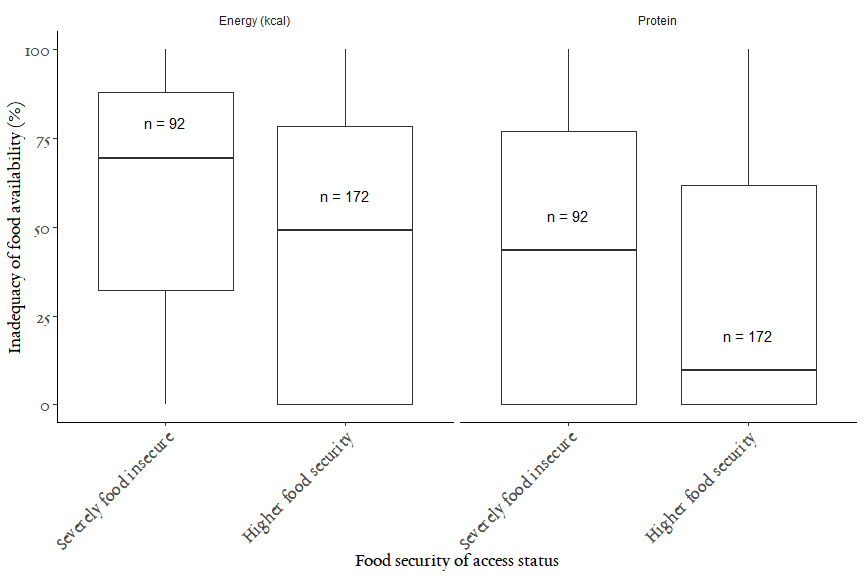
\includegraphics[width=1\textwidth]{Appendix/Ch6_2.png}
  \captionsetup{singlelinecheck = false, justification=justified} %left justify caption
  \caption{Comparison of dietary gaps from farm production and Household Food Insecurity of Access Prevalence (MHFIAP) indicator. This figure is limited to farm dependent households. Food security status is represented by two categories: `Severely food insecure' and an amalgamation of the higher 3 MHFIAP food security categories into the category `Higher food security'. The number of observations are indicated on the figure}
  \label{fig:A_2}
\end{figure}


\vspace*{\fill}
%\newpage

\begin{sidewaystable}[ph!]
  \captionsetup{singlelinecheck = false, justification=justified}
  \caption{Associations between nutrition (dependent variables in columns) and livelihood characteristics and agroecological zone (AEZ). Logistic\textasciicircum{} and negative binomial$^{\dag}$ regressions, displaying the direction of association for statistically significant explanatory variables (n = 6,353)}
  \label{tab:C_7}
  \small
%\begin{tabular}{L{4cm} C{1.5cm} C{1.5cm} C{1.5cm} C{1cm} C{1cm} C{1cm} C{1cm} C{1.5cm} C{1.5cm} C{1.5cm} }
%16.5
\begin{tabularx}{\textwidth}{
p{\dimexpr 0.20\linewidth-2\tabcolsep}
p{\dimexpr 0.08\linewidth-2\tabcolsep}
p{\dimexpr 0.08\linewidth-2\tabcolsep}
p{\dimexpr 0.08\linewidth-2\tabcolsep}
p{\dimexpr 0.08\linewidth-2\tabcolsep}
p{\dimexpr 0.08\linewidth-2\tabcolsep}
p{\dimexpr 0.08\linewidth-2\tabcolsep}
p{\dimexpr 0.08\linewidth-2\tabcolsep}
p{\dimexpr 0.08\linewidth-2\tabcolsep}
p{\dimexpr 0.08\linewidth-2\tabcolsep}
p{\dimexpr 0.08\linewidth-2\tabcolsep}}
\toprule
 & MHFIAP\textasciicircum{} & HDD flush period$^{\dag}$ & HDD lean period$^{\dag}$ & Ca\textasciicircum{} & Fe\textasciicircum{} & Thiamine\textasciicircum{} & Riboflavin\textasciicircum{} & Niacin\textasciicircum{} & Vitamin B6\textasciicircum{} & Vitamin B12\textasciicircum{} \\
\midrule
Intercept & 0.73 (1.15) & 1.17 (0.15)* & 0.41 (0.2) & -2.39 (0.99) & 0.15 (0.67) & 0.18 (0.63) & -0.14 (0.75) & -0.11 (0.86) & 0.42 (0.66) & -2.05 (0.86)* \\
Household inhabitants (adulteq.) & 0.08 (0.04) & 0.02 (0.01)* & 0.04 (0.01)* & 0.08 (0.06)* & 0.02 (0.05) & 0.03 (0.05) & -0.05 (0.06) & 0.01 (0.06) & -0.01 (0.05) & 0.14 (0.06)* \\
Female household head (yes) & -0.23 (0.1)* & -0.01 (0.02) & 0 (0.02) & -0.39 (0.12) & 0.08 (0.11) & 0.07 (0.11) & -0.09 (0.11) & 0.02 (0.11) & 0.15 (0.11) & -0.09 (0.11) \\
Children under 10 (yes) & -0.63 (0.1)* & 0.01 (0.02) & -0.05 (0.02)* & -0.3 (0.11) & 0.01 (0.11) & 0.01 (0.11) & 0.02 (0.1) & -0.05 (0.11) & -0.07 (0.11) & -0.12 (0.11) \\
\arrayrulecolor{black!30}\midrule
Land cultivated (ha) & -0.01 (0.03) & 0 (0.01) & 0 (0.01) & 0.23 (0.09)* & 0.13 (0.06)* & 0.13 (0.06)* & 0.03 (0.08) & 0.11 (0.06) & 0.15 (0.07)* & 0.1 (0.08) \\
Livestock holdings (TLU) & -0.1 (0.03)* & 0.04 (0.02)* & -0.01 (0.01)* & 0.12 (0.05)* & 0.41 (0.13)* & 0.15 (0.05)* & 0.38 (0.12)* & 0.41 (0.14)* & 0.25 (0.06)* & 0.18 (0.05)* \\
Market participation (\% kcal sold) & 0.65 (0.15)* & 0.11 (0.03)* & 0.21 (0.04)* & 0.84 (0.18)* & 0.27 (0.15) & 0.31 (0.15)* & 0.37 (0.16)* & 0.04 (0.16) & 0.31 (0.16)* & 0.75 (0.17)* \\
Off-farm income (yes) & 0.2 (0.09)* & 0.05 (0.02)* & 0.08 (0.02)* & 0.13 (0.1)* & 0.37 (0.09)* & 0.37 (0.09)* & 0.34 (0.09)* & 0.47 (0.1)* & 0.41 (0.09)* & 0.4 (0.1)* \\
Gross income (PPP) & 0.41 (0.06)* & 0.03 (0.01)* & 0.05 (0.01)* & 0.17 (0.05)* & 0.06 (0.04) & 0.06 (0.04) & 0.15 (0.05)* & 0.08 (0.05) & 0.08 (0.05) & 0.16 (0.05)* \\
\arrayrulecolor{black}\bottomrule
%\end{tabular}
\end{tabularx}
\end{sidewaystable}

\vspace*{\fill}



\begin{sidewaystable}[ph!]
\small
\raggedright Table \ref{tab:C_7} continued
\label{tab:C_7_1}

\begin{tabularx}{\textwidth}{
p{\dimexpr 0.20\linewidth-2\tabcolsep}
p{\dimexpr 0.08\linewidth-2\tabcolsep}
p{\dimexpr 0.08\linewidth-2\tabcolsep}
p{\dimexpr 0.08\linewidth-2\tabcolsep}
p{\dimexpr 0.08\linewidth-2\tabcolsep}
p{\dimexpr 0.08\linewidth-2\tabcolsep}
p{\dimexpr 0.08\linewidth-2\tabcolsep}
p{\dimexpr 0.08\linewidth-2\tabcolsep}
p{\dimexpr 0.08\linewidth-2\tabcolsep}
p{\dimexpr 0.08\linewidth-2\tabcolsep}
p{\dimexpr 0.08\linewidth-2\tabcolsep}}
\toprule
 & MHFIAP\textasciicircum{} & HDD flush period$^{\dag}$ & HDD lean period$^{\dag}$ & Ca\textasciicircum{} & Fe\textasciicircum{} & Thiamine\textasciicircum{} & Riboflavin\textasciicircum{} & Niacin\textasciicircum{} & Vitamin B6\textasciicircum{} & Vitamin B12\textasciicircum{} \\
 \midrule
Crop production diversity${\ddag}$ & 0.1 (0.04)* & 0.01 (0.01) & 0.03 (0.01)* & -0.08 (0.04) & 0.1 (0.04)* & 0.1 (0.04)* & -0.01 (0.04) & 0.14 (0.04)* & 0.07 (0.04) & -0.07 (0.04) \\
Livestock product diversity${\ddag}$ & 0.32 (0.05)* & 0.05 (0.01)* & 0.05 (0.01)* & 0.79 (0.06)* & -0.15 (0.05)* & -0.13 (0.05)* & -0.05 (0.05) & -0.07 (0.06) & -0.1 (0.05)* & 0.68 (0.05)* \\
AEZ (sub-)humid{\S} & 0.4 (0.16)* & 0.05 (0.02)* & 0.07 (0.05) & 0.88 (0.2)* & -0.37 (0.18)* & -0.45 (0.18)* & 0.42 (0.19)* & -0.31 (0.2) & -0.48 (0.18)* & 0.76 (0.19)* \\
Household members:AEZ{\S} & NS & NS & 0.02 (0.02) & NS & 0.03 (0.07) & NS & 0.17 (0.08)* & NS & NS & NS \\
Land cultivated:AEZ{\S} & NS & NS & NS & 0.21 (0.12)* & NS & NS & -0.17 (0.11) & 0.28 (0.19) & NS & 0.15 (0.11) \\
Livestock holdings:AEZ{\S} & NS & 0.09 (0.03)* & NS & NS & 0.4 (0.18)* & NS & 0.19 (0.16) & NS & NS & NS \\
Market participation:AEZ{\S} & -1.54 (0.22)* & NS & 0.07 (0.05) & -0.55 (0.24) & NS & NS & NS & NS & NS & -0.45 (0.23)* \\
Crop production diversity:AEZ{\S} & NS & NS & 0.05 (0.01)* & NS & 0.27 (0.05)* & 0.27 (0.05)* & 0.06 (0.05) & 0.28 (0.06)* & 0.26 (0.05)* & NS \\
\arrayrulecolor{black}\bottomrule
\end{tabularx}
\footnotesize
\raggedright
\textasciicircum{} Logistic regression
$^{\dag}$ negative binomial regression
$^{\ddag}$ Number of crop/livestock MHDD categories produced
$^{\S}$ AEZ reference category = semi-arid
\end{sidewaystable}


\begin{figure}[H]
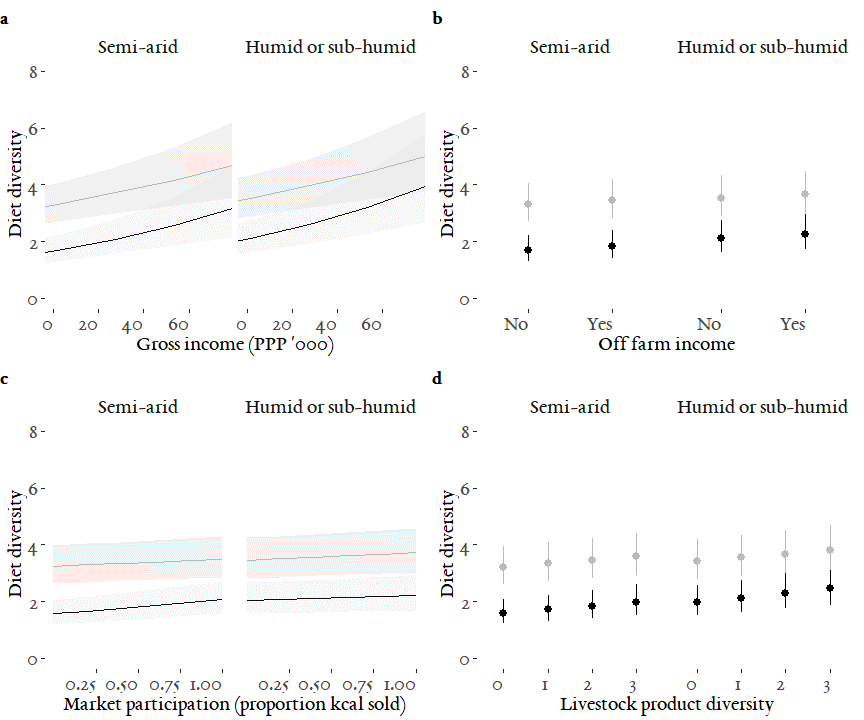
\includegraphics[width=1\textwidth]{Appendix/Ch6_3.png}
    \captionsetup{singlelinecheck = false, justification=justified} %left justify caption
  \caption{Predicted association between other variables and MHDD in the the flush (grey line/point) and lean (black line/point) periods by agroecological zone}
  \label{fig:A_3}
\end{figure}



\begin{table}[H]
  \captionsetup{singlelinecheck = false, justification=justified}
  \caption{Proportion of households in farm types by region}
  \label{tab:C_8}
  \small
\begin{tabularx}{\textwidth}{@{}lYYY@{}}
%  {
%p{\dimexpr 0.35\linewidth-2\tabcolsep}
%p{\dimexpr 0.18\linewidth-2\tabcolsep}
%p{\dimexpr 0.23\linewidth-2\tabcolsep}
%p{\dimexpr 0.23\linewidth-2\tabcolsep}}
\toprule
Farm type~ & East Africa & Central Africa & West Africa \\
\midrule
Specialised cropping & 0.69 & 0.12 & 0.19 \\
Diverse cropping & 0.65 & 0.26 & 0.1 \\
Specialised cropping \& livestock & 0.80 & 0.03 & 0.18 \\
Diverse cropping \& livestock & 0.70 & 0.08 & 0.22 \\
\bottomrule
\end{tabularx}
\end{table}

\begin{figure}[H]
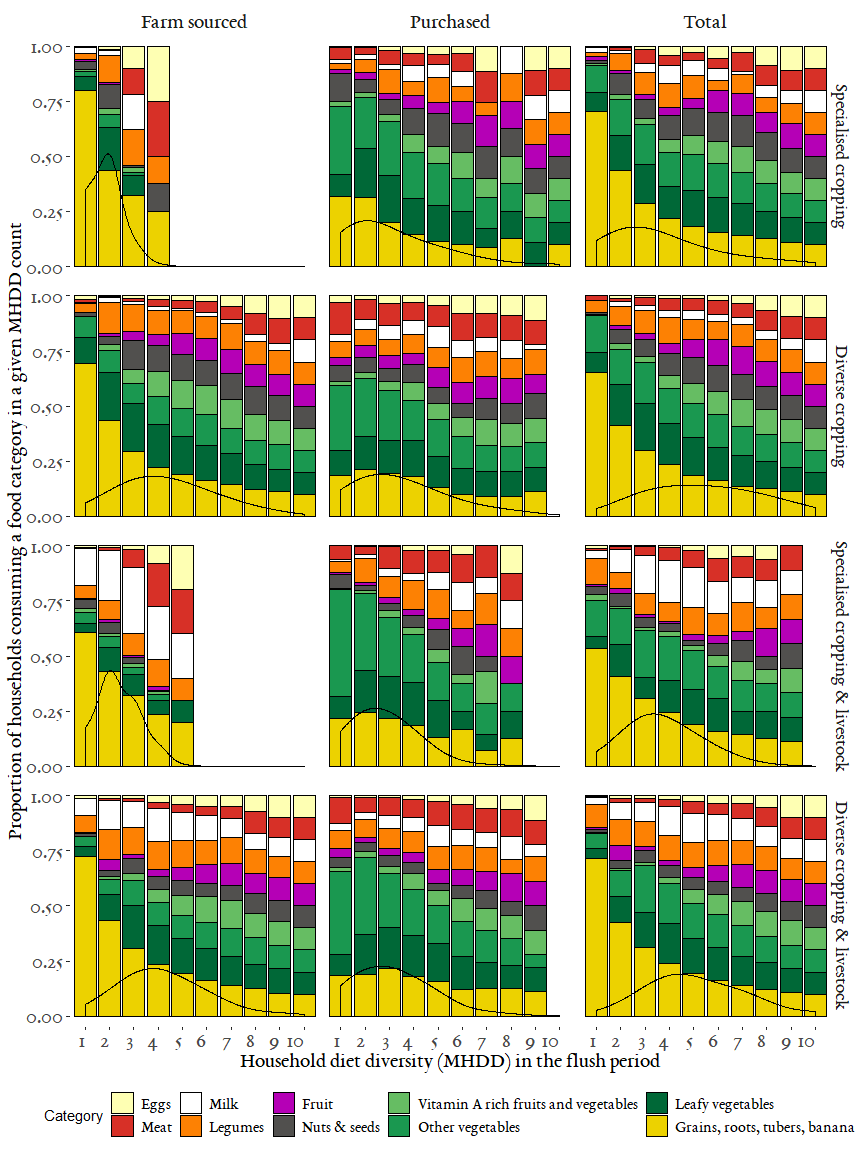
\includegraphics[width=1\textwidth]{Appendix/Ch6_4.png}
    \captionsetup{singlelinecheck = false, justification=justified} %left justify caption
  \caption{Diet diversity: density and proportion of households (n = 6,353) consuming specific food categories by farm type and channel of access in the flush period. The distribution (probability density function) of diet diversity for each period is represented as a black line on the lower half of each figure facet. Food categories are represented by different colours, showing the proportion of households consuming each category at specific diet diversity levels}
  \label{fig:A_4}
\end{figure}

\begin{figure}[H]
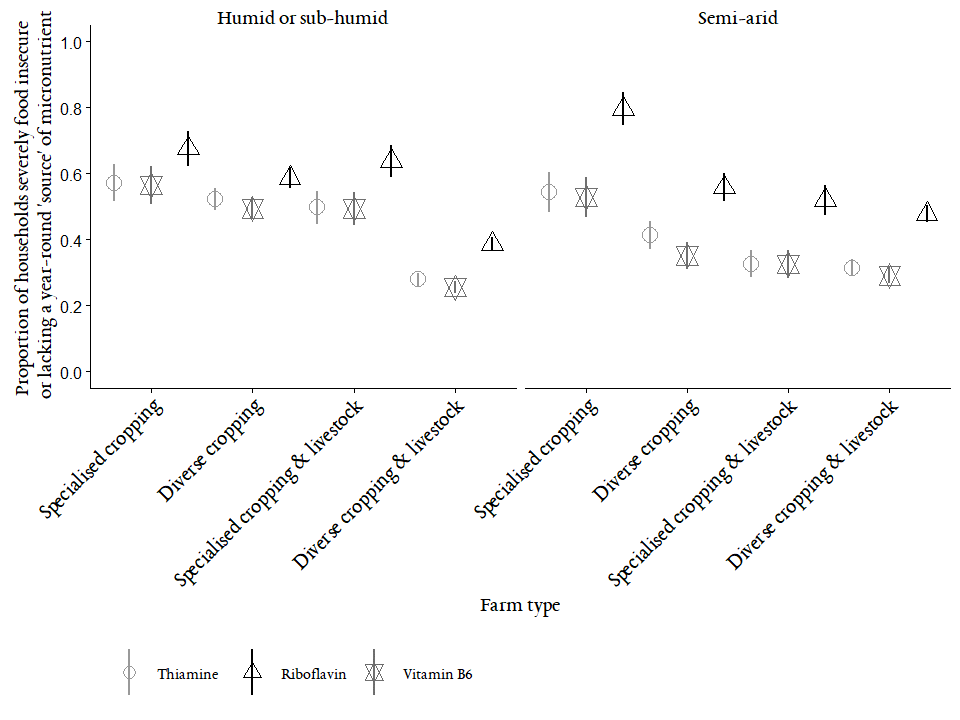
\includegraphics[width=1\textwidth]{Appendix/Ch6_prevalenceOther.png}
    \captionsetup{singlelinecheck = false, justification=justified} %left justify caption
  \caption{Proportion of households (n = 6,353) weighted by population with insecure access to food (MHFIAP) or no `source' of thiamine, riboflavin or vitamin B6 by farm type and agroecological zone. A 95\% confidence interval is represented by vertical lines}
  \label{fig:A_5}
\end{figure}

\begin{itemize}
\item The difference in severe food insecurity prevalence is minimal.

\item Micronutrient estimates are consistently lower for `cropping' households when the threshold is set to 0.5 TLU. The statistically significant difference between `cropping' and `livestock' households, however, remains.

\item A threshold based on animal protein produced was also considered, but is not as suited for a farm type categorisation because it is not as easily observed as TLUs.

\end{itemize}


\begin{table}[H]
  \captionsetup{singlelinecheck = false, justification=justified}
  \caption{Questions asked in MHFIAP and FIES}
  \label{tab:C_10}
  \small
\begin{tabularx}{\textwidth}{
p{\dimexpr 0.37\linewidth-2\tabcolsep}
p{\dimexpr 0.04\linewidth-2\tabcolsep}
p{\dimexpr 0.59\linewidth-2\tabcolsep}}
\toprule
MHFIAP & & FIES \\
\midrule
Did you worry that your household would not have enough food? & & Was there a time when you were worried you would not have enough food to eat because of a lack of money or other resources \\
 & & \\
Was anyone unable to eat your preferred foods due to lack of resources? & & Was there a time when you were unable to eat healthy and nutritious food because of a lack of money or other resources? \\
 & & \\
Did anyone have to eat a limited variety of foods due to lack of resources? & & Was there a time when you ate only a few kinds of foods because of a lack of money or other resources? \\
 & & \\
Did anyone have to eat undesirable foods due to lack of resources? & & Was there a time when you had to skip a meal because there was not enough money or other resources to get food? \\
 & & \\
Did anyone have to eat smaller meals than was felt needed because of limitations in food availability? & & Was there a time when you ate less than you thought you should because of a lack of money or other resources? \\
 & & \\
Did anyone have to eat fewer meals in a day due to a lack of food? & & \\
 & & \\
Was there ever no food of any kind in your household because of a lack of resources? & & Was there a time when your household ran out of food because of a lack of money or other resources? \\
 & & \\
Did anyone go to sleep at night hungry because there was not enough food? & & Was there a time when you were hungry but did not eat because there was not enough money or other resources for food? \\
 & & \\
Did anyone go a whole day and night without eating because there was not enough food? & & Was there a time when you went without eating for a whole day because of a lack of money or other resources? \\
\bottomrule
\end{tabularx}
\end{table}


\begin{table}[H]
  \captionsetup{singlelinecheck = false, justification=justified}
  \caption{Prevalence estimates derived from Martin-Pr\'{e}vel et al. (2015)}
  \label{tab:C_11}
  \small
\begin{tabularx}{\textwidth}{@{}lYYYYYYYY@{}}
%  {
%p{\dimexpr 0.29\linewidth-2\tabcolsep}
%p{\dimexpr 0.09\linewidth-2\tabcolsep}
%p{\dimexpr 0.09\linewidth-2\tabcolsep}
%p{\dimexpr 0.09\linewidth-2\tabcolsep}
%p{\dimexpr 0.09\linewidth-2\tabcolsep}
%p{\dimexpr 0.1\linewidth-2\tabcolsep}
%p{\dimexpr 0.09\linewidth-2\tabcolsep}
%p{\dimexpr 0.09\linewidth-2\tabcolsep}
%p{\dimexpr 0.09\linewidth-2\tabcolsep}}
\toprule
 & & \multicolumn{7}{l}{Probability of adequacy (mean)} \\
 & n & Ca & Fe & Thiamine & Riboflavin & Niacin & Vitamin B6 & Vitamin B12 \\
 \midrule
Burkina Faso 1 & 182 & 0.03 & 0.23 & 0.39 & 0.08 & 0.17 & 0.53 & 0.07 \\
Burkina Faso 2 & 407 & 0.23 & 0.51 & 0.43 & 0.47 & 0.71 & 0.36 & 0.03 \\
Mali & 102 & 0.04 & 0.53 & 0.6 & 0.28 & 0.31 & 0.67 & 0.17 \\
Uganda 1 & 452 & 0.06 & 0.08 & 0.84 & 0.33 & 0.76 & 0.97 & 0.18 \\
Uganda 2 & 954 & 0.07 & 0.13 & 0.77 & 0.56 & 0.73 & 0.83 & 0.03 \\
Total & 2097 & 197 & 464 & 1422 & 918 & 1392 & 1542 & 152 \\
Weighted probability adequate & & 0.09 & 0.22 & 0.68 & 0.44 & 0.66 & 0.74 & 0.07 \\
Weighted deficiency prevalence & & 0.91 & 0.78 & 0.32 & 0.56 & 0.34 & 0.26 & 0.93 \\
\bottomrule
\end{tabularx}
\end{table}


\vspace{1cm}

\begin{table}[H]
  \captionsetup{singlelinecheck = false, justification=justified}
  \caption{
  Association between farm-household-diet characteristics and farm type -- non-livestock oriented vs. livestock orientated. Mixed-effects regressions.
  }
  \label{tab:C_12}
  \small
\begin{tabular}{L{5cm} C{2.5cm} C{2.5cm} C{2cm} C{2cm}}
\toprule
Dependent variable & Intercept estimate (SE) & $\hat{\beta}$\textsubscript{livestock} estimate (SE)$^{\dag}$ &  \\
\midrule
Household inhabitants (Adult eq) & 5.46 (0.51) & 0.92 (0.13) & * \\
Land cultivated (ha) & 1.95 (0.49) & 0.72 (0.20) & * \\
Livestock holdings (TLU) & 3.18 (4.08) & 8.64 (1.16) & * \\
Progress out of poverty & 33.68 (6.73) & 3.45 (0.56) & * \\
MHDDS flush period$^{\ddag}$ & 1.86 (0.08) & 0.04 (0.02) & * \\
MHDDS lean period$^{\ddag}$ & 1.44 (0.10) & 0.12 (0.02) & * \\
Milk consumed in lean period$^\psi$ & -1.33 (0.71) & 1.39 (0.11) & * \\
Meat consumed in lean period$^\psi$ & -0.80 (0.46) & 0.45 (0.11) & * \\
Eggs consumed in lean period$^\psi$ & -2.08 (0.39) & 0.63 (0.11) & * \\
\bottomrule
\end{tabular}
\footnotesize
\raggedright
%\caption*{
\\
95\% CI does not cross zero \\
$^{\dag}$Reference category is `non-livestock oriented farm types' \\
$^{\ddag}$Negative binomial regression \\
$^\psi$Logistic regression. Reference category is `did not consume'
\end{table}


\begin{table}[H]
  \captionsetup{singlelinecheck = false, justification=justified}
  \caption{
  Association between farm-household-diet characteristics and farm type -- specialised cropping vs. diverse. Mixed-effects linear regressions.
  }
  \label{tab:C_12}
  \small
\begin{tabular}{L{5cm} C{2.5cm} C{2.5cm} C{2cm} C{2cm}}
\toprule
Dependent variable & Intercept estimate (SE) & $\hat{\beta}$\textsubscript{diverse} estimate (SE)$^{\dag}$ &  \\
\midrule
Market participation (proportion kcal sold) & 0.25 (0.05) & 0.07 (0.01) & * \\
Crop income (PPP) & 8.74 (21.30) & 0.49 (7.63) & \\
Vitamin A rich consumed in lean period$^\psi$ & 0.31 (0.41) & 0.51 (0.08) & * \\
Dark leafy veg consumed in lean period$^\psi$ & 2.27 (0.58) & 1.02 (0.11) & * \\
Other veg consumed in lean period$^\psi$ & 2.50 (0.53) & 0.51 (0.11) & * \\
Fruit consumed in lean period$^\psi$ & -0.32 (0.59) & 0.52 (0.08) & * \\
Nuts/seeds consumed in lean period$^\psi$ & -0.34 (0.08) & 0.50 (0.08) & * \\
\bottomrule
\end{tabular}
\footnotesize
\raggedright
%\caption*{
\\
95\% CI does not cross zero \\
$^{\dag}$Reference category is `non-livestock oriented farm types'
\end{table}




\begin{table}[H]
  \captionsetup{singlelinecheck = false, justification=justified}
  \caption{
  Association between severe food insecurity / micronutrient access and diverse cropping, livestock keeping households in humid \& sub-humid zones. Mixed-effects logistic regressions.
  }
  \label{tab:C_13_2}
  \small
\begin{tabular}{L{5cm} C{2.5cm} C{2.5cm} C{2cm} C{2cm}}
\toprule
Dependent variable & Intercept estimate (SE) & $\hat{\beta}$\textsubscript{diverse \& livestock} estimate (SE)$^{\dag}$ &  \\
\midrule
Severely food insecure$^{\ddag}$ & -0.86 (0.73) & -0.15 (0.16) & * \\
Calcium$^{\ddag}$ & -2.27 (0.99) & 0.98 (0.16) & * \\
Iron$^{\ddag}$ & -0.05 (0.37) & 0.67 (0.13) & * \\
Thiamine$^{\ddag}$ & 0.01 (0.32) & 0.67 (0.13) & * \\
Riboflavin$^{\ddag}$ & -0.27 (0.37) & 0.52 (0.19) & * \\
Niacin$^{\ddag}$ & -0.27 (0.48) & 0.63 (0.15) & * \\
Pyridoxine$^{\ddag}$ & 0.16 (0.39) & 0.61 (0.13) & * \\
Cobalamin$^{\ddag}$ & -1.58 (0.57) & 0.85 (0.15) & * \\
\bottomrule
\end{tabular}
\footnotesize
\raggedright
%\caption*{
\\
95\% CI does not cross zero \\
$^{\dag}$Reference category is `specialised or no livestock component' \\
$^{\ddag}$Reference category is `did not consume'
\end{table}

\begin{table}[H]
  \captionsetup{singlelinecheck = false, justification=justified}
  \caption{
  Association between severe food insecurity / micronutrient access and specialised cropping, livestock keeping farm types in arid semi-arid zones. Mixed-effects logistic regressions.
  }
  \label{tab:C_13_3}
  \small
\begin{tabular}{L{5cm} C{2.5cm} C{2.5cm} C{2cm} C{2cm}}
\toprule
Dependent variable & Intercept estimate (SE) & $\hat{\beta}$\textsubscript{livestock} estimate (SE)$^{\dag}$ &  \\
\midrule
Chronic hunger$^{\ddag}$ & 0.34 (0.71) & 0.64 (0.14) & * \\
Calcium$^{\ddag}$ & -1.96 (1.27) & 0.99 (0.19) & *\\
Iron$^{\ddag}$ & 0.87 (0.92) & 0.17 (0.15) &  \\
Thiamine$^{\ddag}$ & 0.83 (0.81) & 0.18 (0.15) &  \\
Riboflavin$^{\ddag}$ & -0.24 (1.25) & 0.23 (0.17) &  \\
Niacin$^{\ddag}$ & 0.64 (0.92) & 0.27 (0.59) &  \\
Pyridoxine$^{\ddag}$ & 1.17 (1.03) & 0.08 (0.16) &  \\
Cobalamin$^{\ddag}$ & -2.01 (1.27) & 1.23 (0.18) & * \\
\bottomrule
\end{tabular}
\footnotesize
\raggedright
%\caption*{
\\
95\% CI does not cross zero \\
$^{\dag}$Reference category is `no livestock component' \\
$^{\ddag}$Reference category is `did not consume'
\end{table}



\begin{table}[H]
  \captionsetup{singlelinecheck = false, justification=justified}
  \caption{
  Association between farm-household-diet characteristics and the presence of children. Mixed-effects regressions.
  }
  \label{tab:C_14}
  \small
\begin{tabular}{L{5cm} C{2.5cm} C{2.5cm} C{2cm} C{2cm}}
\toprule
Dependent variable & Intercept estimate (SE) & $\hat{\beta}$\textsubscript{children} estimate (SE)$^{\dag}$ &  \\
\midrule
Household inhabitants (Adult eq) & 4.38 (0.45) & 2.21 (0.11) & * \\
Age of household head & 66.39 (11.33) & -3.45 (4.15) & \\
Land cultivated (ha) & 2.09 (0.49) & 0.42 (0.17) & * \\
Livestock holdings (TLU) & 4.48 (4.85) & 4.85 (0.99) & * \\
Gross income (PPP) & 1479.95 (411.92) & 0.60 (8.73) &  \\
Progress out of poverty & 43.00 (7.46) & -9.61 (0.46) & * \\
\bottomrule
\end{tabular}
\footnotesize
\raggedright
%\caption*{
\\
95\% CI does not cross zero \\
$^{\dag}$Reference category is `no children' \\
$^{\ddag}$Negative binomial regression
\end{table}


\begin{table}[H]
  \captionsetup{singlelinecheck = false, justification=justified}
  \caption{
  Association between chronic hunger (severe food insecurity) and micronutrient access and scale for diverse cultivating, livestock keeping farm types in humid \& sub-humid zones. Mixed-effects logistic regressions.
  }
  \label{tab:C_15}
  \small
\begin{tabular}{L{5cm} C{2.5cm} C{2.5cm} C{2cm} C{2cm}}
\toprule
Dependent variable & Intercept estimate (SE) & $\hat{\beta}$\textsubscript{medium-large} estimate (SE)$^{\dag}$ &  \\
\midrule
Chronic hunger$^{\ddag}$ & -0.37 (0.32) & -0.70 (0.20) & * \\
Calcium$^{\ddag}$ & -1.57 (1.21) & 0.42 (0.26) & * \\
Iron$^{\ddag}$ & 0.38 (0.74) & 0.25 (0.24) & \\
Thiamine$^{\ddag}$ & 0.49 (0.64) & 0.28 (0.23) & \\
Riboflavin$^{\ddag}$ & 0.07 (0.60) & -0.04 (0.20) &  \\
Niacin$^{\ddag}$ & -0.05 (0.84) & 0.62 (0.27) & * \\
Pyridoxine$^{\ddag}$ & 0.53 (0.75) & 0.41 (0.22) &  \\
Cobalamin$^{\ddag}$ & -1.05 (0.98) & 0.45 (0.24) &  \\
\bottomrule
\end{tabular}
\footnotesize
\raggedright
%\caption*{
\\
95\% CI does not cross zero \\
$^{\dag}$Reference category is `small scale' \\
$^{\ddag}$Reference category is `did not consume'
\end{table}


\begin{table}[H]
  \captionsetup{singlelinecheck = false, justification=justified}
  \caption{
  Association between chronic hunger (severe food insecurity) and micronutrient access and scale for specialised cropping, livestock keeping farm types in arid semi-arid zones. Mixed-effects logistic regressions.
  }
  \label{tab:C_16}
  \small
\begin{tabular}{L{5cm} C{2.5cm} C{2.5cm} C{2cm} C{2cm}}
\toprule
Dependent variable & Intercept estimate (SE) & $\hat{\beta}$\textsubscript{medium-large} estimate (SE)$^{\dag}$ &  \\
\midrule
Chronic hunger$^{\ddag}$ & -0.84 (5.93) & 0.45 (0.22) & * \\
Calcium$^{\ddag}$ & -1.99 (1.91) & 0.30 (0.30) & \\
Iron$^{\ddag}$ & 1.04 (1.01) & 0.50 (0.26) & * \\
Thiamine$^{\ddag}$ & 1.04 (1.00) & 0.49 (0.27) & * \\
Riboflavin$^{\ddag}$ & -0.56 (1.54) & 0.44 (0.28) &  \\
Niacin$^{\ddag}$ & 0.97 (1.08) & 0.30 (0.27) &  \\
Pyridoxine$^{\ddag}$ & 1.08 (0.93) & 0.55 (0.27) & * \\
Cobalamin$^{\ddag}$ & -1.57 (2.02) & -0.11 (0.31) & \\
\bottomrule
\end{tabular}
\footnotesize
\raggedright
%\caption*{
\\
95\% CI does not cross zero \\
$^{\dag}$Reference category is `small scale' \\
$^{\ddag}$Reference category is `did not consume'
\end{table}



\addcontentsline{toc}{chapter}{Acknowledgements}
%\chapter{Acknowledgements}%The star removes the entry from the bibliography - add manually for the reading version
{\Large\textbf{Acknowledgements}}
\chaptermark{Acknowledgements}

I am grateful to the many people who have inspired, challenged and supported me throughout my PhD trajectory. I extend my gratitude and indebtedness first and foremost to the rural households that shared a small part of their stories with us. I also wish to express my gratitude to the enumerators who guided these detailed and at times sensitive discussions.

To my promotor, Imke de Boer, thank you for asking such challenging questions, for the frank and open discussions and for hosting me. To your credit, you have cultivated a high performing and supportive work culture, for which I am glad to have been a part. To my co-promotor Simon Oosting, thank you for your support, for sharing your insights and for your dedicated input right up to submission. To my co-promotor Mark van Wijk, your leadership and collaborative spirit has provided exciting opportunities to better understand the circumstances of rural households across Africa, Asia and south-central America. I am grateful for your insights, feedback and encouragement. You have shaped and enriched this thesis and have given me the freedom to make this research my own. Thank you. 

To my unofficial supervisor, Mats Lannerstad, you were instrumental in the formation of this PhD project and have been an active contributor throughout my PhD trajectory. Your leadership in the CLEANED project provided me with immense opportunities to develop my research capacities. I would also like to thank you for the brainstorming sessions, critical feedback and well-timed bouts of laughter.  

To my other highly esteemed co-authors, it has been a pleasure to work with you all. I would like to take the opportunity to single out a few individuals in this public acknowledgement. The development and refinement of the RHOMIS tool was driven by James Hammond, with many, many hours of dutiful labour. It was great to collaborate and share in a genuine commitment to improve the standard of living in rural communities. I would like to express my gratitude to Mario Herrero, Nils Teufel, Todd Rosenstock, Jacob van Etten, Tim Pagella, Bernard Vanlauwe, Augustine Ayantunde and Ken Giller. As co-authors, you provided thought provoking comments and as scientists you have set the bar high -- thank you. Thank you to Jessica Bogard and Mary Ng'endo for the discussions on human nutrition. Thank you to George Sayula and Viviane Yameogo for your dedication to the communities in Lushoto and northern Burkina Faso. Thank you to Pietro Carpena, David Baines and the team at TreeAID for their tireless efforts to support the most vulnerable rural communities. 

From my early research career in Australia, I would like to thank Helen Scarborough and Phil Hone; thank you to Tim Ada, and the fine people in the `Agribusiness team', the Rutherglen research centre and the Ellinbank research center; thank you to John Moran; thank you to Zita Ritchie and the `grads'; thank you to Robyn Alders and the Kyeema team, and; thank you to Richard Eckard for your support.  

Thank you to my colleagues in ILRI for sharing your wealth of knowledge and for your camaraderie. To name but a few, I would like to thank Isabelle Baltenweck, Amos Omore, Ben Lukuyu, Karen Marshall, Jane Poole, An Notenbaert and Carlos Queros; Thomas Randolph and Delia Grace Randolph; Todd Crane, Katie Tavennar and Stanley Ng'ang'a; Edmund Githoro, Simon Mugatha, Eunice Kariuki, Emmanuel Kithuna, Julius Githingi, Leone Mawa, Gregory Sikumba and Jusper Ronno; Beth Njoroge, Pauline Aluoch and Assenath Kabugi; Asaah Ndambi and Patric Brandt. Thank you to Polly Ericksen for your support during my PhD.

Thank you to Pierre Gerber for providing such interesting research topics earlier in my career and for taking an interest in my PhD trajectory. Thank you to Theun Vellinga for the very early brainstorming on my PhD.

I would like to thank the WIAS staff. I thank the scientific director Johan van Leeuwen for his leadership and for taking an active role in the delivery of PhD courses. Thank you to the WIAS secretariat Janneke van Seters, Marianne Bruining and Bernie Coenders. Thank you to my study advisor Guido Bosch. Thank you to Walter Gerrits and Michiel Kleerebezem for the critical feedback on my proposal.

To the team at APS, I would like to express my sincere and heartfelt gratitude for welcoming and supporting me. To Eddie Bokkers, Kees van Reenen and Henk Udo, thank you for your leadership in the group. To Theo Viets and Fokje Steenstra, thank you for your tireless efforts in the group and for modelling what it is to be educators with impact. To Lia Verheijen, thank you for your support and good humour. I have really enjoyed the discussions (without boundaries), walks and outings with APS. I am grateful for your focus on (human) animal welfare -- you have been a kind and generous source of support. Thank you to Aart van der Linden, Abigail Muscat, Aimable Uwizeye, Akke Kok, Alejandro Parodi, Brain Akakpo, Cindy Klootwijk, Corina van Middelaar, Evelien de Olde, Hannah van Zanten, Heleen van Kernebeek, Iris Boumans, Laura Webb, Louise Kremer, Margret Wenker, Ollie van Hal, Pim Mostert, Pim Post, Raimon Ripoll Bosch, Salome `Sally' Migose, Simon Nyokabi, Titis Apdini, Windi al Zahra and Ylva Ran.

Thank you to my colleagues in the Plant Production Systems group. Jannike Wichern, I really enjoyed our in-depth discussions on food security and rural livelihoods -- it has been great to be on this journey with you. Joost van Heerwaarden, Wytze Marinus, Eva Thuijsman, Anne de Valença, I enjoyed our discussions. I am grateful to the team at CDI for providing opportunities to carry out my pedogeological training. In particular, thank you to Ted Schrader and Diane Bosch. Thank you to Bas Engel for the enlightening discussions on statistics. Thank you to Emmanual Koyano for translating the summary of this thesis into Kiswahili. 

I would also like to express my sincere gratitude to the members of the committee for taking the time to evaluate my thesis and to participate in the public defense.

Thank you to my dear parents for cultivating my curiosity, diligence, and compassion. Thank you to my brothers, sisters, nephews and nieces for the inspiration that you have given me. Thank you to Roland Fraval, Shari Cohen and the good people of Brunswick who made me feel at home in my hometown during the analysis phase of my PhD. Rafiki zangu kutoka Afrika Mashariki -- asanteni sana. Ulinikaribishwa na hunifundisha sana sana. Pamoja na neema ya Mungu, natumaini tutaboresha maisha ya watu wanaopunguzwa.     

%\lipsum[1-9]



\addcontentsline{toc}{chapter}{Summary}
%\chapter{Summary}
{\Large\textbf{Summary}}
\chaptermark{Summary}
\label{cha:Summary}

Malnutrition affects the quality of life for a substantial portion of the human population. The incidence of adverse health effects due to chronic undernourishment and micronutrient deficiencies are substantially higher in sub-Saharan Africa (SSA) compared to the rest of the world. The individual and societal implications for such nutritional gaps are borne disproportionately by the rural population, indicated by the consistently higher prevalence of stunting in rural SSA. Members of rural households are both vulnerable to the health burdens that stem from food insecurity and central to improving the availability and affordability of a diversity of wholesome foods for both rural and urban markets.

It has been estimated that much of the chronic and hidden hunger that we see today can be alleviated by implementing a suite of nutrition-specific interventions at a cost of US\$9.6 billion per annum. The effectiveness of such investments can be accelerated with complementary food system-based interventions. However, such food system-based interventions are hampered by a limited understanding of the prevalence of food insecurity, the spatial distribution of food insecurity, and the associations between food insecurity and rural livelihoods. The primary objective of this thesis was to describe, analyse and understand food security in rural landholding households in predominantly mixed crop-livestock agricultural systems of sub-Saharan Africa (SSA). The secondary objective was to improve the methodological basis of household level food security studies.

The rural household multi-indicator survey (RHOMIS) tool was developed to describe and analyse the circumstances of rural households -- including food security status. \textbf{Chapter 2} describes the design principles and core modules of the RHOMIS tool. The RHOMIS tool aims to adhere to the principles of being time-efficient, utilitarian, user-friendly, flexible and reliable. The core modules include farm characteristics, household composition, food security, progress out of poverty and `gender'. \textbf{Chapter 2} provides a preliminary evaluation of the time-efficiency and user-friendliness of the RHOMIS tool. The duration of RHOMIS is half that of comparable surveys. The ease of enumeration was evaluated favourably for each module, with over 50\% of interviews being perceived as `easy' by the interviewer.

A critical evaluation of the quality of data produced by rural household surveys is then carried out in \textbf{Chapter 3}. This chapter evaluates the credibility, consistency and reliability of data collected using three different farm household surveys deployed in four African countries. Several limitations in data quality were identified. First, variables which might be considered `easy to estimate' had instances of non-credible observations. For example, in the food security and food self-sufficiency indicators, between 29\% and 57\% of observations in the World Bank's `living standards measurement survey' were deemed beyond credible bounds. In contrast, the shorter and more targeted survey tool, RHOMIS, performed better -- with 25\% of observations beyond credible bounds. Measurements of maize yields and land area owned were found to be less reliable than other variables such as household inhabitants and livestock holdings. This lack of reliability has implications for monitoring food security status, poverty status and the land productivity of households. Despite the limitations in data quality, our analysis shows that if the same farm households are followed over time, the sample sizes needed to detect substantial changes are in the order of hundreds of surveys, and not in the thousands. Chapter 3 concludes that targeted and systematised household surveys are essential in detecting differences and changes in rural communities.

The RHOMIS tool was then used to quantify changes in livelihoods and food security status in an urban linked, high potential region of Tanzania. \textbf{Chapter 4} incorporates paired observations from 20 villages in Lushoto district, Tanzania, over three years. This chapter evaluates the extent to which changes in livelihoods, poverty and food security were taking place in such a short span of time. Households in the study site adaptively responded to local and national circumstances and can be grouped in four clusters, namely: `Rising high value crop', `Rising livestock', `Subsisting mixed' and `Subsisting staples'. A substantial portion of households in the study site made changes to their livelihoods over the short three-year period of observation. Changes in land ownership, livestock-holdings and high value crop production were most likely related to market opportunities and personal circumstances, rather than to direct interventions. Several households made strategic changes by expanding land ownership, planting perennial crops and investing in exotic cattle breeds; many households tactically utilised their land for diversified, mixed crop-livestock production. The majority of households, however, had either remained stable or were scaling back to subsistence farming. \textbf{Chapter 4} finds that the complex risk management strategies and market responsiveness demonstrated by the `Rising' clusters are at odds with single focus activities that external organisations tend to promote.

Subsequently, instances of chronic and hidden hunger were analysed in two subtly contrasting regions of Burkina Faso. \textbf{Chapter 5} describes and analyses the household composition, farm systems and food security status in these regions. Food security indicators were enumerated for two periods to account for the temporal variability throughout the year. Diet diversity (a proxy for hidden hunger) was disaggregated by channel of access to better understand food sourcing behaviour. The results of this chapter show that in both provinces, the ability to purchase food is what differentiates the more food secure households from their less food secure counterparts. This finding does not detract from the utility of subsistence production -- where consumption of own-farm sourced food catered for 91\% of the annual energy requirements in Yatenga province and 72\% in Seno province. Further, households were observed to be pursuing market-oriented strategies in combination with production diversification. Production diversification was not driving differences in diet diversity in this instance but was likely to reduce risk exposure to climatic or economic shocks.

\textbf{Chapter 6} draws on a large sample of rural landholding households across SSA to estimate the prevalence of dietary gaps and to understand their associations with rural livelihoods and food sourcing behaviour throughout the year. As many as 40\% of households were classified as chronically hungry in the lean period. Prevalence of micronutrient dietary gaps were high, ranging from 35\% of households lacking daily sources of pyridoxine, and 68\% lacking daily sources of calcium. Vulnerability to dietary gaps differed by household composition, livelihood characteristics and agro-ecological zone (AEZ). Market participation, livestock product diversity, crop diversity, gross income and off-farm income were all associated with chronic and hidden hunger -- differing by AEZ. Any given livelihood characteristic had a limited impact on food security indicators. Rather, it is the combination of these livelihood characteristics and the agro-ecological production potential that drive the availability of food and income. Households with a livestock component to their farm consumed more milk, meat and eggs (sources of calcium, riboflavin and vitamin B12). Dairy, fruit and vitamin A-rich produce were predominantly accessed through the farm channel -- more so by diverse cropping households. The results of Chapter 6 suggest that households fail to purchase food categories that nutritionally complement their own agricultural products. Furthermore, households with a livestock component to their farm were found to have a lower prevalence of chronic and hidden hunger.

Methodological considerations and empirical findings of this thesis are further evaluated in a general discussion. The general discussion in \textbf{Chapter 7} summarises the progress that has been made in harmonising rural household surveys through the RHOMIS tool. The RHOMIS tool is now available in 9 languages and has been localised to 48 sub-national locations in SSA, South-East Asia and, South and Central America. A community of practice has formed around the use of the tool which provides opportunities for further methodological developments in sampling, validation, alternative modes of data collection, improved enumeration and modelling of women's empowerment and improvements in measuring food and nutrition security.

This thesis has drawn upon a total of 8,257 household interviews, conducted in 14 projects to describe and analyse food and nutrition security in rural landholding households. \textbf{Chapter 7} reiterates the high prevalence rates of chronic and hidden hunger identified in this thesis, noting the variability between and within regions. The factors identified to be associated with food and nutrition security in Chapters 4, 5 and 6 are then analysed and discussed further. In extended analyses, the gender of household head and stage of life were found to be associated with the number of household inhabitants and thus influence nutritional requirements and food security status. The high prevalence of food insecurity, the complexity of associations and the failure to nutritionally complement own-production with purchases have implications for developing effective interventions. The discussion concludes that programs can be designed as `packages' of agricultural and non-agricultural interventions to maximise adoption and maximise the positive impact on food and nutrition security throughout the year.

\phantomsection

\addcontentsline{toc}{chapter}{Muhtasari}
%\chapter{Summary}
{\Large\textbf{Muhtasari}}
\chaptermark{Muhtasari}
\label{cha:Muhtasari}

Hali duni ya afya inayosababishwa na lishe duni na upungufu wa vurutubisho muhimu ni kubwa sana katika nchi za kusini mwa jangwa la Sahara ikilinganishwa na sehemu nyingine duniani. Athari za madhara binafsi na madhara kwa jamii yanayosababishwa na utofauti huu mkubwa wa kilishe mara nyingi hubebwa na jamii zinazoishi vijijini zikiashiriwa na uwepo mkubwa zaidi wa utapiamlo kwenye mazingira ya vijiji ikilinganishwa na mazingira ya mijini. Jamii zinazoishi kwenye mazingira ya vijijini ziko katika hali hatarishi zaidi ya mizigo ya magonjwa yanayotokana na upungufu wa chakula na tatizo la kuwezesha upanikanaji na uthamani wa mazao mbalimbali ya chakula kwenye masoko ya mijini na vijijini. Inakadiriwa kuwa kiasi kikubwa cha njaa sugu iliyojificha (utapiamlo) tunayoiona wakati huu inaweza kuondolewa kwa kufuata afua zinazolenga lishe bora kwa gharama ya dola bilioni 9.6 kwa mwaka. Matokeo mazuri ya uwekezaji kama huu yanaweza kuongezewa kasi kwa kutumia mfumo wenye hatua zenye kutumia vyakula mbadala ingawa mifumo yenye kutumia afua zinazotumia vyakula mbadala inaharibiwa na uelewa mdogo wa uwepo wa upungufu mkubwa na chakula, mgawanyo wa kutokuwa na ulinzi wa chakula maeneo mengi na uhusiano kati ya uhaba wa chakula na maisha ya vijijini.

Lengo kuu la tafiti hii lilikuwa ni kuelezea, kutathmini na kuelewa uhaba uwepo wa chakula kwenye kaya zilizopo maeneo ya vijijini hasa hasa ambayo huzalisha mazao mchanganyiko, na mifumo ya wakulima wafugaji chini ya jangwa la Sahara. Lengo la pili lilikuwa ni kuboresha misingi ya njia za masomu yanayohusiana na ulinzi wa chakula. 
Nyenzo za ukusanyaji wa takwimu tofauti za tathmini ya viashiria mablimbali vya maisha vijijini zilitengenzwa kuelezea na kutathmini hali halisi za kaya zilizoko maeneo hayo pamoja na hali halisi ya ulinzi wa chakula. 

\textbf{Sura ya 2} inaelezea kanuni na muundo wa msingi wa nyenzo za ukusanyaji wa takwimu hizi za tathmini. Nyenzo za ukusanyaji wa takwimu hizi zina lengo la kuzingatia kanuni za kuwa na ufanisi wa muda, zenye urahisi wa kutumia, kubadilishwa na kuaminika. Vipengele vya msingi vya nyenzo za ukusanyaji wa takwimu hizi ni pamoja na sifa za shamba, muundo wa kaya, lishe, maendeleo ya umaskini na 'jinsia'.

\textbf{Sura ya 3} inatoa tathmini ya awali ya ufanisi wa muda na ni rafiki kwa mtumiaji. Muda wa ambao nyenzo za ukusanyaji wa takwimu hizi hutumia ni takribani nusu ya nyenzo za ukusanyaji wa takwimu za utafiti zinazofanana. Vilevile zaidi ya asilimia hamsini ya mahojiano yameonekana kuwa rahisi kwa mhojiwa. Sura ya 3 inaonyesha maadili yasiyo ya kawaida, thabiti na yenye takwimu za kuaminika zilizokusanywa kwa kwenye tafiti tatu za kilimo kwa ngazi ya kaya katika nchi nne za Afrika. Vikwazo kadhaa vya ubora wa takwimu vilibainishwa. Kwanza, majibu ambayo watafiti wanafikiri ni 'rahisi kupatikana' yalikuwa na matukio ya makosa. Kwa mfano, viashiria vya lishe na upatikanaji wa chakula cha kutosha, kati ya asilimia 29 na 57 ya tathmini zilizofanyika za hali ya ubora wa maisha kwa `viwango vya maisha' vya bank kuu ya dunia zilionekana kuwa na makosa ikilinganishwa na nyenzo za kukusanya takwimu za mfupi na ambazo huchukua walengwa zaidi, (RHOMIS) zilifanya vizuri kwa asilimia zaidi 25\% ya tathmini.
Vilevile, upimaji wa mavuno ya mahindi, na ukubwa wa mashamba ulionekana kuwa hauna uhakika zaidi ikilinganishwa na vigezo vingine kama vile idadi ya watu na umiliki wa mifugo. Ukosefu wa kuaminika wa nyenzo za ukusanyaji wa takwimu hauthiri tathmini za ukosefu wa lishe, hali ya umasikini na mavuno ya mazao kwa kaya. Licha ya mapungufu katika ubora wa takwimu, uchambuzi wetu unaonyesha kuwa ikiwa kaya zinafuatiliwa, ukubwa wa sampuli unaohitajika kutoa matokeo sahihi sio wa kaya maelfu bali ni wa kaya mamia. Sura ya 3 inahitimisha kuwa, uchunguzi wa kaya unaofuata utaratibu sahihi ni muhimu sana katika huhakikisha kuwa kupata tawimu sahihi za tofauti na mabadiliko katika jamii zilizoko vijijini.

Nyenzo za ukusanyaji wa takwimu za RHOMIS zilikuwa kilikuwa zinatumiwa kupima mabadiliko ya hali ya maisha na hali ya lishe nchini Tanzania katika nyanja zinazohusiana na masoko na zina uwezo mzuri wa uzalishaji wa takwimu sahihi. \textbf{Sura ya 4} inafafanua uchunguzi uliofanyika kwenye vijiji 20 vilivyoainishwa katika wilaya ya Lushoto, Tanzania kwa zaidi ya miaka mitatu.
Sura hii inachunguza kiwango cha mabadiliko ya maisha, umasikini na lishe kilichotokea kwa kipindi cha muda mfupi majumbani. Tafiti za majumbani zilizofanyika kwenye tovuti hutegemea mazingira ya ndani ya nchi husika ambayo yanaweza kugawanywa katika makundi manne, yaani: `kuongezeka kwa thamani ya mazao', `kuongezeka kwa thamani ya mifugo', `mazao mchanganyiko ya kujikimu' and `mazao makuu ya kujikimu'. Sehemu kubwa ya kaya katika tovuti ya utafiti zilifanya mabadiliko ya maisha yao kwa muda mfupi wa uchunguzi wa miaka mitatu.
Mabadiliko katika umiliki wa ardhi, ufugaji wa mifugo na uzalishaji wa mazao ya thamani ya juu yalikuwa na uwezekano mkubwa wa kuhusiswa na fursa za masoko na hali za kibinafsi, badala ya hali za kijamii. Kaya kadhaa zilifanya mabadiliko ya kimkakati katika kupanua umiliki wa ardhi, kuwekeza katika mifugo na kukuza mazao ya thamani ya juu; kaya nyingi zilitumia ardhi yao kwa ajili ya kilimo cha mazao mbalimbali, na uzalishaji wa mifugo. hata hivyo, kaya nyingi, zilikuwa imara au zilikuwa zikitumia mazao yaliyozalishawa nyumbani. Sura ya 4 inabainisha kuwa mikakati ya usimamizi na ufumbuzi wa masoko imewezeshwa sana na makundi ya vyakula 'yanayochipukia' ikilinganishwa na kazi za ambazo zinahimizwa sana na mashirika ya nje. 

Vilevile, matukio ya `ukosefu wa nishati' na `ukosefu wa virutubishi' yalichambuliwa katika mikoa miwili tofauti ya Burkina Faso. \textbf{Sura ya 5} inaelezea na inachambua muundo wa kaya, mifumo ya kilimo na hali ya lishe katika mikoa hii. Viashiria vya lishe vilichapishwa kwa muda wa vipindi viwili kwenye kwa utofauti wa mwaka mzima. Njia za upatikanaji wa chakula mchanganyiko (kipimo cha `ukosefu ya virutubishi') zilitofautiana. Matokeo ya sura hii yanaonyesha tofauti mablimabali kujipatia chakula ikilinganishwa na uwezo wa kipato wa kaya kwenye mikoa yote. Matokeo haya hayakupunguza thamani ya chakula kinachotumiwa kutoka mashambani ambacho huchangia asilimia 91 ya mahitaji mwaka ya nishati katika jimbo la Yatenga na asilimia 72 katika jimbo la Seno. Zaidi ya hayo, kaya zilionekana kuzingatia mikakati inayotokana na soko, pamoja na aina mablimbali za uzalishaji. Hivyo basi, uzalishaji mbadala huenda ukapunguza hatari ya hali ya hewa au hatari ya kiuchumi.

\textbf{Sura ya 6} inatathmini sampuli kubwa ya kaya za vijijini nchini Afrika ya Kusini ili kukadiria upungufu ya chakula na kuelewa vyanzo vya kipato na maisha ya vijijini na upatikanaji wa chakula kwa mwaka mzima. Takriban asilimia 38 ya kaya zilionekana kuwa na `njaa kali'. Hali ya kuenea kwa upungufu wa chakula ulikuwa ni ya juu, kutoka takribani asilimia 41 ya kaya kukosa vyanzo vya chakula chenye madini chuma kila siku na madini ya `thiamine' na asilimia 72 kutokuwa na vyanzo vya kila siku vya vitamini B12. Mapungufu ya chakula hutofautiana na mfumo wa kaya sifa ya sifa nyanda za ki-agroikolojia. Aina za masoko, utofauti wa mifugo, utofauti wa mazao, mapato ya jumla na mapato ya nje ya kilimo yalihusishwa na `upungufu wa virutubishi' ikilinganishwa na nyanda za ki-agroikolojia. Tabia moja pekee ilikuwa na athari ndogo juu ya viashiria vya usalama wa chakula. Badala yake, mchanganyiko wa tabia hizi pamoja na eneo la ki-agroekolojia huchangia mabadiliko katika mapato na upatikanaji wa chakula. Kaya zilizo kuwa na mifugo zilitumia maziwa zaidi, nyama na mayai (vyanzo vya madini chuma, riboflavin na vitamini B12) Maziwa, matunda na vitamini A, hupatikana kwa wingi kadri mazao ya mashamba yanavyoongezeka. Matokeo ya Sura ya 6 yanaonyesha kwamba kaya hazijinunulii makundi ya chakula ili kukidhi mahitaji yao yote ya lishe. Zaidi ya hayo, kaya zilizo na mifugo zilikuwa na lishe bora kuliko nyingine.

Masuala ya njia ya utafiti na matokeo ya utafiti huu yanatathminiwa zaidi katika mjadala wa jumla. Mjadala wa jumla katika \textbf{Sura ya 7} unaonesha muhtasari wa maendeleo ambayo yamefanyika katika kuunganisha tafiti za kaya za vijijini kwa njia ya nyenzo za ukusanyaji wa takwimu za RHOMIS. Nyenzo za ukusanyaji wa takwimu za RHOMIS sasa zinapatikana katika lugha 9 na zimefanyika maeneo 48 ya kitaifa katika nchini Afrika ya kusini, Kusini-mashariki mwa Asia na, kusini na katikati mwa Marekani. Kwa kuwa kuna watumiaji wengi wenye mahitaji ya nyenzo hii, kuna fursa za maendeleo zaidi ya ya nyenzo hii ikiwa ni pamoja na sampuli, uthibitisho, njia mbadala za ukusanyaji wa takwimu, kuelewa uwezo wa wanawake na kuboresha upimaji lishe. Tafiti hii imefanya jumla ya mahojiano ya kaya 8,257, katika miradi 14 inayolenga kuelezea na kuchambua masuala ya lishe ya kaya vijijini. 

\textbf{Sura ya 7} inaelezea viwango vya juu vya kuenea kwa `upungufu wa nishati' na `upungufu wa virutubishi', akibainisha tofauti kati ya mikoa na maeneo ndani ya nchi husika. Sababu ambazo zinahusiana na lishe katika Sura ya 4, 5 na 6 zimeonesha kufuatiliwa na kujadiliwa zaidi. Uchambuzi zaidi umeonesh kuwa jinsia, ukuu wa kaya na hali ya maisha vimehusishwa zaidi na idadi ya watu kwenye kaya na basi kuathiri mahitaji ya lishe na hali ya `kukosa lishe'. Hiyo ni mchanganyiko wa sifa hizi za maisha ambazo huamua hali ya usalama wa chakula kwa mwaka mzima. Matokeo haya yote yana maana katika kuendeleza hatua za ufanisi. Mjadala huu unahitimisha kuwa programu zinaweza kuundwa kama 'vikundi' ya hatua za kilimo na zisizo za kilimo ili kuboresha hatua za kupunguza lishe kwa mwaka mzima.

\phantomsection

\thispagestyle{empty}\cleartoleftpage


%% Back Matter

\addcontentsline{toc}{chapter}{About the author}
%\chapter{About the author} 
{\Large\textbf{About the author}}
\chaptermark{About the author}

\small
Simon Fraval was born on the 30th of December 1983 in Ascot, England. In 2007, Simon earned a Bachelor of Commerce with honors in economics from Deakin University (Melbourne, Australia). His minor thesis was titled `Determining financial support for Australian electricity generators in an emission constrained economy'. 

Between 2008 and 2012, Simon was employed by the state government of Victoria, Australia. During his tenure, he was stationed at the head office in Melbourne, the Rutherglen lamb and viticulture research centre, and the national centre for dairy research and development. His research interests centred on agricultural trade, including topics of production trends, market access, animal welfare of live exports and the environmental impacts of exported livestock products. In 2010, Simon co-authored an article published in the Journal of Dairy Science, titled \textit{`The water footprint of dairy products: case study involving skim milk powder'}. In 2012, Simon presented his work titled \textit{`Sustainable Value Chain Analysis: Victorian lamb exported to the USA'} to the IFAMR conference in Frankfurt, Germany. 

In 2012, Simon joined the International Livestock Research Institute (ILRI). Soon after moving to Nairobi, Kenya, Simon took part in a Comprehensive Africa Agriculture Development Programme (CAADP) meeting, discussing the alignment between policy and research agendas. He then focused his research on the quantification and mitigation of greenhouse gas (GHG) emissions in smallholder diary production, with research sites in western Kenya. In collaboration with the FAO, the Kenyan ministry of agriculture and Unique Forestry, Simon co-authored a methodology for incentivising GHG mitigation, titled \textit{`Smallholder dairy methodology: Draft Methodology for Quantification of GHG Emission Reductions from Improved Management in Smallholder Dairy Production Systems using a Standardized Baseline'}. 

Simon continued his research in ILRI under the auspice of the project titled `Comprehensive Livestock Environmental Assessment for Improved Nutrition, a Secured Environment and Sustainable Development' (CLEANED). In a collaboration between ILRI, CIAT, SEI and CSIRO, the CLEANED project sought to provide a method to estimate the environmental impact of livestock interventions in low and middle income countries prior to implementation. Simon was involved throughout the research process, from conceptual development, piloting, analysis and reporting. Simon led the GHG and biodiversity components of the framework and co-led participatory GIS activities in Kenya and Tanzania.    

In 2015, Simon began the field work for his PhD. Hosted by ILRI and the Animal Production Systems group of Wageningen University \& Research, Simon sought to understand and describe the nature of food security in rural sub-Saharan Africa. During the process of his PhD, Simon co-authored five peer-reviewed articles and two book chapters. Simon has also been active in the research community -- reviewing journal articles and presenting his work.
Simon's research interests include topics related to food security, rural livelihoods, environmental impact assessment and remote sensing. 

%\lipsum[1-3]


\newpage

\small
{\normalsize\textbf{Peer-reviewed journal publications}}
%\vspace{-0.5cm}


Ridoutt, B. G., Williams, S. R. O., Baud, S., Fraval, S., \& Marks, N. (2010). Short communication: The water footprint of dairy products: case study involving skim milk powder. \textit{Journal of Dairy Science}, 93(11), 5114–7. doi:10.3168/jds.2010-3546

Hammond, J., Fraval, S., van Etten, J., Suchini, J. G., Mercado, L., Pagella, T., Frelat, R., Lannerstad, M., Douxchamps, D., Teufel, N., Valbuena, D., \& van Wijk, M. T. (2017). The Rural Household Multi-Indicator Survey (RHoMIS) for rapid characterisation of households to inform climate smart agriculture interventions: Description and applications in East Africa and Central America. \textit{Agricultural Systems, 151}, 225–233. doi:10.1016/j.agsy.2016.05.003

Ng'ang'a, S., Ritho, C., Herrero, M., \& Fraval, S. (2018). Household-oriented benefits largely outweigh commercial benefits derived from cattle in Mabalane District, Mozambique. \textit{The Rangeland Journal, 40(6)}, 565–576. doi:10.1071/RJ17115

Tavenner, K., Fraval, S., Omondi, I., \& Crane, T. A. (2018). Gendered reporting of household dynamics in the Kenyan dairy sector: trends and implications for low emissions dairy development. Gender, Technology and Development, 22(1), 1–19. doi:10.1080/09718524.2018.1449488

Fraval, S., Hammond, J., Wichern, J., Oosting, S. J., de Boer, I. J. M., Teufel, N., Lannerstad, M., Waha, K., Pagella, T., Rosenstock, T. S., Giller, K. E., Herrero, M., Harris, D., \& van Wijk, M. T. (2018). Making the most of imperfect data: a critical evaluation of standard information collected in farm household surveys. \textit{Experimental Agriculture}, 1–21. doi:10.1017/S0014479718000388.

Fraval, S., Hammond, J., Lannerstad, M., Oosting, S. J., Sayula, G., Teufel, N., Silvestri, S., Poole, E. J., Herrero, M., \& van Wijk, M. T. (2018). Livelihoods and food security in an urban linked, high potential region of Tanzania: Changes over a three year period. \textit{Agricultural Systems, 160 (January 2018)}, 87–95. doi:10.1016/j.agsy.2017.10.013

{\normalsize\textbf{Submitted manuscripts}}

%\vspace{-0.5cm}
Fraval, S., Yameogo, V., Ayantunde, A., Hammond, J., de Boer, I. J. M., Oosting, S. J., \& van Wijk, M. T. (submitted). Pathways to food security in rural Burkina Faso. \textit{Food Security}

Fraval, S., Hammond, J., Bogard, J. R., Ng'endo, M., van Etten, J., Herrero, M., Oosting, S. J., de Boer, I. J. M., Lannerstad, M., Teufel, N., Lamanna, C., Rosenstock, T. S., Pagella, T., Vanlauwe, B., Dontsop-Nguezet, P. M., Baines, D., Carpena, P., Njingulula, P., Okafor, C., Wichern, J., Ayantunde, A., Bosire, C., Chesterman, S., Kihoro, E., Rao, J., Skirrow, T., Steinke, J., Stirling, C. M., Yameogo, V., \& van Wijk, M. T. (submitted). Dietary gaps in sub-Saharan Africa: prevalence and implications for agricultural interventions. \textit{Global Food Security}

Ritzema, R., van Wijk, M., Phengsavanh, P., Hammond, J., Fraval, S., Hok, L., Thi Minh Long, C., Bolliger, A., \& Douxchamps, S. (submitted). Household-level drivers of dietary diversity in transitioning agricultural systems: Evidence from the Greater Mekong Subregion
Stanley northern Kenya. \textit{Agricultural systems}



{\normalsize\textbf{Book chapters}}

%\vspace{-0.5cm}
Fraval, S., van Middelaar, C., Ridoutt, B., \& Opio, C. (2018). Life Cycle Assessment of Food Products. In P. Ferranti, E. M. Berry, \& J. R. Anderson (Eds.), \textit{Encyclopedia of Food Security and Sustainability} (Vol. 3, pp. 488–496). Elsevier. doi:10.1016/B978-0-08-100596-5.21427-3

Wijk, M. T. Van, Hammond, J., Frelat, R., \& Fraval, S. (2018). Unequal Access to Land: Consequences for the Food Security of Smallholder Farmers in Sub Saharan Africa. In P. Ferranti, E. M. Berry, \& J. R. Anderson (Eds.), \textit{Encyclopedia of Food Security and Sustainability} (pp. 1–6). Elsevier. doi:10.1016/B978-0-12-812687-5.22311-3



{\normalsize\textbf{Other scientific publications}}

%\vspace{-0.5cm}
Opio, C., Gerber, P., Baltenweck, I., Fraval, S., Mbae, R., Kessei, L., Wilkes, A., Tennigkeit, T., Marroquin, L., Baumann, T., \& Hardy, P. (2016). \textit{Smallholder dairy methodology: Draft Methodology for Quantification of GHG Emission Reductions from Improved Management in Smallholder Dairy Production Systems using a Standardized Baseline}.

Morris, J., Fraval, S., Githoro, E., Ran, Y., \& Mugatha, S. (2015). \textit{Comprehensive Livestock Environmental Assessment for Improved Nutrition, a Secured Environment and Sustainable Development along Livestock and Aquaculture Value Chains Project: PGIS workshop summary report}. (2015 No. 05). Stockholm.

{\normalsize\textbf{Conference proceedings}}

%\vspace{-0.5cm}
Fraval, S., Marks, N., Fearne, A., \& Ridoutt, B. G. (2011). Sustainable Value Chain Analysis: Victorian  lamb exported  to  the USA. \textit{The Road to 2050: Sustainability as a Business Opportunity}. Frankfurk: IFAMR. Available on \url{https://www.ifama.org/2011-Frankfurt}

Fraval, S., Hammond, J., Bogard, J. R., Ng'endo, M., van Etten, J., Herrero, M., Oosting, S. J., de Boer, I. J. M., Lannerstad, M., Teufel, N., Lamanna, C., Rosenstock, T. S., Pagella, T., Vanlauwe, B., Dontsop-Nguezet, P. M., Baines, D., Carpena, P., Njingulula, P., Okafor, C., Wichern, J., Ayantunde, A., Bosire, C., Chesterman, S., Kihoro, E., Rao, J., Skirrow, T., Steinke, J., Stirling, C. M., Yameogo, V., \& van Wijk, M. T. (2018). Food access channels in tropical sub-Saharan Africa. In \textit{Accelerating the End of Hunger and Malnutrition}. Bangkok: IFPRI-FAO. Available on \url{https://www.ifpri-faobangkokconference.org/files/2018/11/Slide43.jpg}

Fraval, S., Hammond, J., Bogard, J. R., Ng'endo, M., van Etten, J., Herrero, M., Oosting, S. J., de Boer, I. J. M., Lannerstad, M., Teufel, N., Lamanna, C., Rosenstock, T. S., Pagella, T., Vanlauwe, B., Dontsop-Nguezet, P. M., Baines, D., Carpena, P., Njingulula, P., Okafor, C., Wichern, J., Ayantunde, A., Bosire, C., Chesterman, S., Kihoro, E., Rao, J., Skirrow, T., Steinke, J., Stirling, C. M., Yameogo, V., \& van Wijk, M. T. (2019). Dietary gaps in rural sub-Saharan Africa. \textit{4th International Congress on Hidden Hunger}. Stuttgart: SNFS. Available on \url{http://hiddenhunger.net}

Teufel, N., Hammond, J., Fraval, S., \& van Wijk, M. T. (2018). Dynamics of food security and livelihood strategies in Eastern Africa. In \textit{Strengthening food and nutrition security through a Planetary Health lens in resource-limiting settings conference}. Dar es Salaam: University of Sydney. Available on \url{https://sydney.edu.au/vetscience/research/Nkuku4U/images/Nkuku4U-program.pdf}
\normalsize

\phantomsection


\addcontentsline{toc}{chapter}{Education certificate}
%\thispagestyle{empty}
%\begin{flushleft}
%\end{flushleft}
%\chapter{WIAS education certificate}
%\begin{minipage}[c]{.55\textwidth}
%\end{minipage}
%\begin{minipage}[c]{.35\textwidth}
%\begin{flushright}
%\vspace{0pt}\includegraphics[width=4.6cm,height=4.6cm]{WIASlogo.png}
%\end{flushright}
%\end{minipage}%
%\vspace{-1cm}
%\bigskip

{\Large\textbf{WIAS education certificate}}
\vspace{4mm}
%\small
\hrule
\textbf{Completed training and supervision plan$^1$}
\vspace{2mm}
\hrule
\begin{tabular}[t]{l l}
\begin{minipage}{0.73\textwidth}
\textbf{The Basic Package (1.8 ECTS)}
%\vspace{-2mm} %A quick hackaround
\begin{itemize}[nolistsep, topsep=0cm] %Topsep doesn't work See answer here https://stackoverflow.com/questions/1061112/eliminate-space-before-beginitemize
    \item WIAS Introduction Day (2017)
    \item WGS course 'Ethics and philosophy in life sciences' (2017)
\end{itemize}
%\\
\vspace{2mm}
\textbf{Disciplinary Competences (11.6 ECTS)}
%\vspace{-2mm}
\begin{itemize}[nolistsep,topsep=0cm]
    \item Resilience of living systems (2018)
    \item Writing PhD research proposal
    \item Soil4life: sustainable soil management (2016)
    \item Machine learning (2016)
    \item Data science (2015)
\end{itemize}
%\\
\vspace{1mm}

\end{minipage}
&
%\begin{minipage}{0.23\textwidth}
\includegraphics[width=3.6cm,height=3cm]{WIASlogo.png}
%\end{minipage}
\end{tabular}

\textbf{Professional Competences (9.4 ECTS)}
\vspace{-2mm}
\begin{itemize}[nolistsep,topsep=0cm]
    \item WGS PhD workshop carousel (2018)
    \item Didactic skills: Teaching outside academia (2017)
    \item How to review a scientific paper (2017)
    \item Scientific writing (2015)
    \item Swahili (2015)
\end{itemize}

\textbf{Presentation Skills (4.0 ECTS)}
\vspace{-2mm}
\begin{itemize}[nolistsep,topsep=0cm]
    \item Congress hidden hunger, Stuttgart, Germany (2019)
    \item WIAS science day, Wageningen, the Netherlands (2019)
    \item Accelerating the End of Hunger and Malnutrition, Bangkok, Thailand (2018)
    \item WaCASA, Wageningen, the Netherlands (2018)
    \item RHOMIS user group workshop, Wageningen, the Netherlands (2018)
    \item Global agenda for action on climate change, Nairobi, Kenya (2013)
\end{itemize}

\textbf{Teaching Competences (4.2 ECTS)}
\vspace{-2mm}
\begin{itemize}[nolistsep,topsep=0cm]
    \item Guest lecture and support in Future Livestock Systems course (2018)
	\item Assistance with supervising MSc student (2015)
    \item Leading tutorials and online discussions in two undergraduate courses (2007, 2011)
\end{itemize}

\vspace{5mm}

\hrule
\textbf{Total: 31.0}
\vspace{2mm}
\hrule
\small
$^1$With the activities listed the PhD candidate has complied the educational requirements set by the Graduate School of Wageningen Institute of Animal Sciences (WIAS) of Wageningen University \& Research, which comprises of a minimum of 30 ECTS (European Credit Transfer and accumulation System). One ECTS equals a study load of 28 hours.
\normalsize

\phantomsection

\renewcommand{\headrulewidth}{0pt}
\cleartoleftpage

\addcontentsline{toc}{chapter}{Colophon}
\thispagestyle{empty}\thispagestyle{empty}
\vspace*{1cm}

{\Large\textbf{Colophon}}
\chaptermark{}
\\
\\
This research received funding from the CGIAR Research Programs on `Livestock and Fish', `Climate Change, Agriculture and Food Security' (CCAFS) and `Maize' and its donors and by support of the American People provided to the Feed the Future Innovation Lab for Sustainable Intensification through the United States Agency for International Development (USAID).

Several donors and organisations supported this research indirectly. A full list of contributing donors and organisations can be found in Appendix Table \ref{tab:C_2}.

The views expressed in this thesis cannot be taken to reflect the official opinions of these organisations.


Images used in this thesis:
\begin{itemize}
\item Shared plate by Albert Gonzalez Farran from UNAMID

\item Food items were downloaded from pngmart.com

\item Plough with oxen was sourced from the WUR image library

\item Woman harvesting grain was sourced from unsplash.com

\item Chapter 5 photo by Ollivier Girard from CIFOR 

\item Chapter 7 photo from ILRI
\end{itemize}


All other images were taken by the author or acknowledged in-text

\vspace*{\fill}
Cover design by Simon Fraval and Fokje Steenstra

Printed by ProefschriftMaken, www.proefschriftmaken.nl

\phantomsection
\end{document}
